\documentclass[
%paper=5.5in:8.5in,
a5paper,
]{scrbook} 
\title{Le comte de Monte-Cristo, tome~4}
\usepackage{montecristovf}


\begin{document}
\frontmatter
\pagestyle{plain}
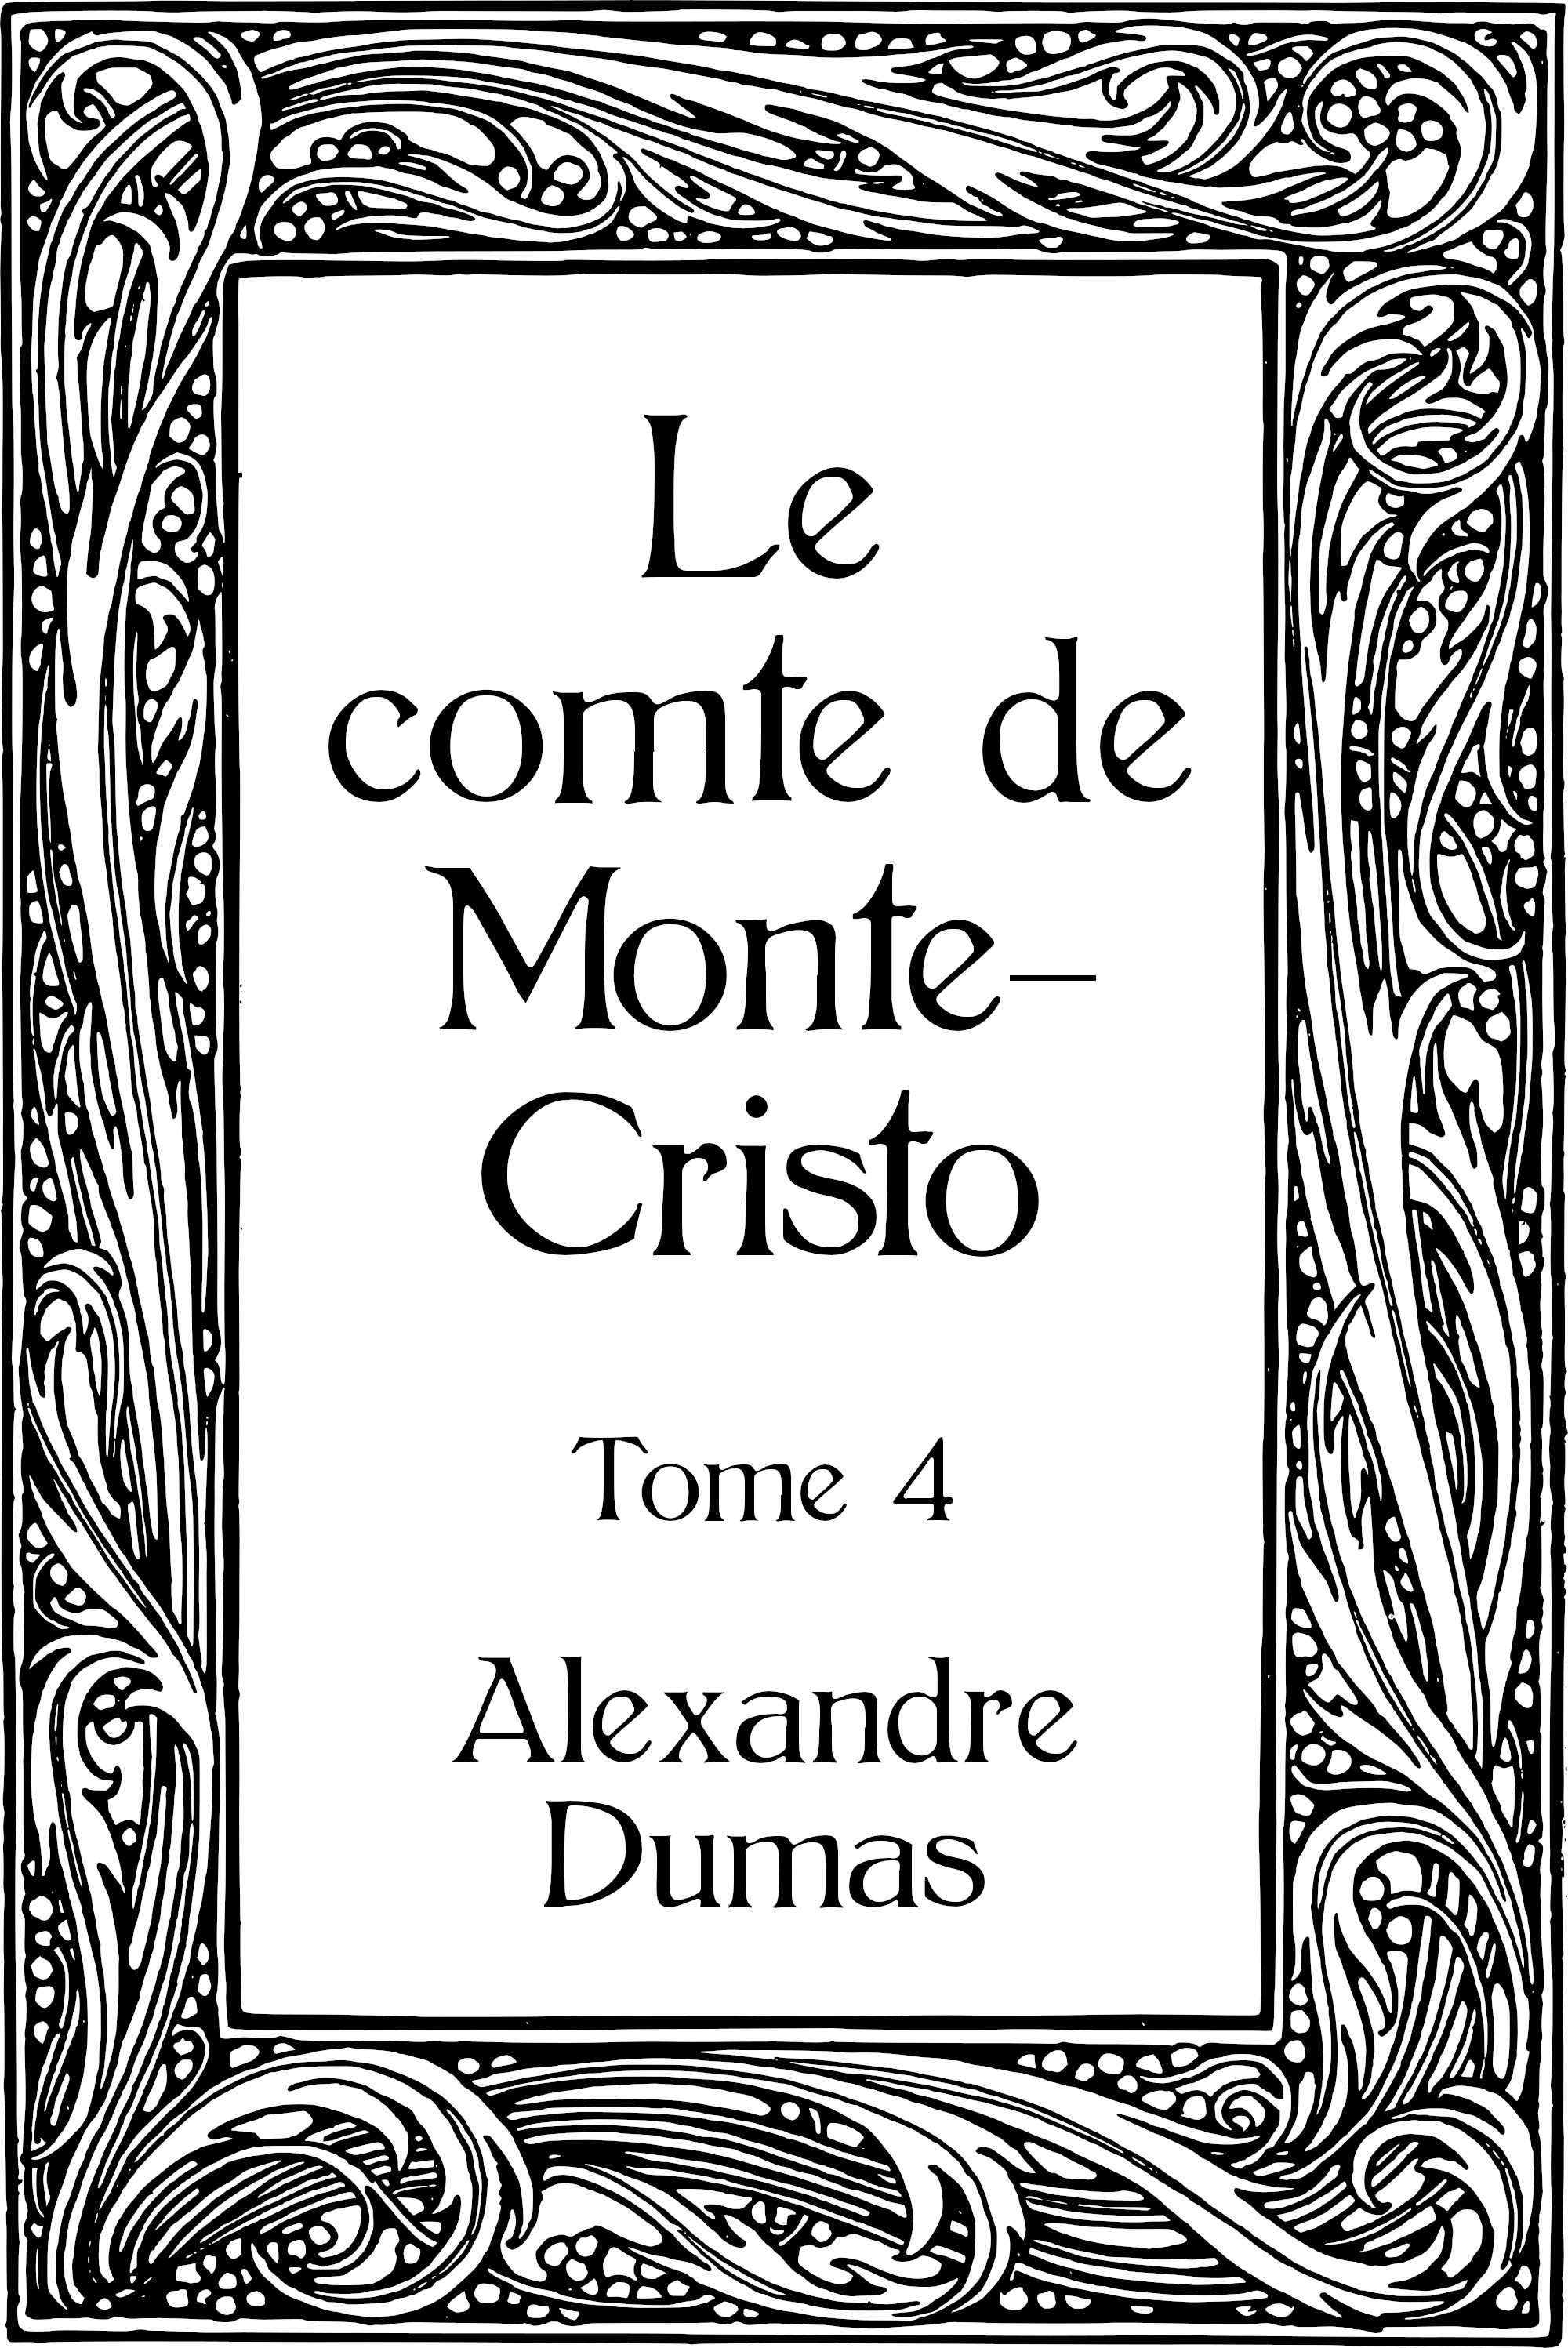
\includepdf[width=\basicwidth]{titlepagevf4.jpg}
\KOMAoptions{headings=openleft}
\tableofcontents
 

 
\mainmatter
\pagestyle{headings}
\KOMAoptions{headings=openright}
\setcounter{chapter}{84}
\chapter{The Journey} 

 \lettrine{M}{onte} Cristo uttered a joyful exclamation on seeing the young men together. <Ah, ha!> said he, <I hope all is over, explained and settled.> 

\zz
 <Yes,> said Beauchamp; <the absurd reports have died away, and should they be renewed, I would be the first to oppose them; so let us speak no more of it.> 

 <Albert will tell you,> replied the count <that I gave him the same advice. Look,> added he. <I am finishing the most execrable morning's work.> 

 <What is it?> said Albert; <arranging your papers, apparently.> 

 <My papers, thank God, no,—my papers are all in capital order, because I have none; but M. Cavalcanti's.> 

 <M. Cavalcanti's?> asked Beauchamp. 

 <Yes; do you not know that this is a young man whom the count is introducing?> said Morcerf. 

 <Let us not misunderstand each other,> replied Monte Cristo; <I introduce no one, and certainly not M. Cavalcanti.> 

 <And who,> said Albert with a forced smile, <is to marry Mademoiselle Danglars instead of me, which grieves me cruelly.> 

 <What? Cavalcanti is going to marry Mademoiselle Danglars?> asked Beauchamp. 

 <Certainly! do you come from the end of the world?> said Monte Cristo; <you, a journalist, the husband of renown? It is the talk of all Paris.> 

 <And you, count, have made this match?> asked Beauchamp. 

 <I? Silence, purveyor of gossip, do not spread that report. I make a match? No, you do not know me; I have done all in my power to oppose it.> 

 <Ah, I understand,> said Beauchamp, <on our friend Albert's account.> 

 <On my account?> said the young man; <oh, no, indeed, the count will do me the justice to assert that I have, on the contrary, always entreated him to break off my engagement, and happily it is ended. The count pretends I have not him to thank;—so be it—I will erect an altar \textit{Deo ignoto}.> 

 <Listen,> said Monte Cristo; <I have had little to do with it, for I am at variance both with the father-in-law and the young man; there is only Mademoiselle Eugénie, who appears but little charmed with the thoughts of matrimony, and who, seeing how little I was disposed to persuade her to renounce her dear liberty, retains any affection for me.> 

 <And do you say this wedding is at hand?> 

 <Oh, yes, in spite of all I could say. I do not know the young man; he is said to be of good family and rich, but I never trust to vague assertions. I have warned M. Danglars of it till I am tired, but he is fascinated with his Luccanese. I have even informed him of a circumstance I consider very serious; the young man was either charmed by his nurse, stolen by gypsies, or lost by his tutor, I scarcely know which. But I do know his father lost sight of him for more than ten years; what he did during these ten years, God only knows. Well, all that was useless. They have commissioned me to write to the major to demand papers, and here they are. I send them, but like Pilate—washing my hands.> 

 <And what does Mademoiselle d'Armilly say to you for robbing her of her pupil?> 

 <Oh, well, I don't know; but I understand that she is going to Italy. Madame Danglars asked me for letters of recommendation for the \textit{impresari}; I gave her a few lines for the director of the Valle Theatre, who is under some obligation to me. But what is the matter, Albert? you look dull; are you, after all, unconsciously in love with Mademoiselle Eugénie?> 

 <I am not aware of it,> said Albert, smiling sorrowfully. Beauchamp turned to look at some paintings. 

 <But,> continued Monte Cristo, <you are not in your usual spirits?> 

 <I have a dreadful headache,> said Albert. 

 <Well, my dear viscount,> said Monte Cristo, <I have an infallible remedy to propose to you.> 

 <What is that?> asked the young man. 

 <A change.> 

 <Indeed?> said Albert. 

 <Yes; and as I am just now excessively annoyed, I shall go from home. Shall we go together?> 

 <You annoyed, count?> said Beauchamp; <and by what?> 

 <Ah, you think very lightly of it; I should like to see you with a brief preparing in your house.> 

 <What brief?> 

 <The one M. de Villefort is preparing against my amiable assassin—some brigand escaped from the gallows apparently.> 

 <True,> said Beauchamp; <I saw it in the paper. Who is this Caderousse?> 

 <Some Provençal, it appears. M. de Villefort heard of him at Marseilles, and M. Danglars recollects having seen him. Consequently, the procureur is very active in the affair, and the prefect of police very much interested; and, thanks to that interest, for which I am very grateful, they send me all the robbers of Paris and the neighbourhood, under pretence of their being Caderousse's murderers, so that in three months, if this continues, every robber and assassin in France will have the plan of my house at his fingers' ends. I am resolved to desert them and go to some remote corner of the earth, and shall be happy if you will accompany me, viscount.> 

 <Willingly.> 

 <Then it is settled?> 

 <Yes, but where?> 

 <I have told you, where the air is pure, where every sound soothes, where one is sure to be humbled, however proud may be his nature. I love that humiliation, I, who am master of the universe, as was Augustus.> 

 <But where are you really going?> 

 <To sea, viscount; you know I am a sailor. I was rocked when an infant in the arms of old Ocean, and on the bosom of the beautiful Amphitrite; I have sported with the green mantle of the one and the azure robe of the other; I love the sea as a mistress, and pine if I do not often see her.> 

 <Let us go, count.> 

 <To sea?> 

 <Yes.> 

 <You accept my proposal?> 

 <I do.> 

 <Well, viscount, there will be in my courtyard this evening a good travelling britzka, with four post-horses, in which one may rest as in a bed. M. Beauchamp, it holds four very well, will you accompany us?> 

 <Thank you, I have just returned from sea.> 

 <What? you have been to sea?> 

 <Yes; I have just made a little excursion to the Borromean Islands\footnote{Lake Maggiore. }.> 

 <What of that? come with us,> said Albert. 

 <No, dear Morcerf; you know I only refuse when the thing is impossible. Besides, it is important,> added he in a low tone, <that I should remain in Paris just now to watch the paper.> 

 <Ah, you are a good and an excellent friend,> said Albert; <yes, you are right; watch, watch, Beauchamp, and try to discover the enemy who made this disclosure.> 

 Albert and Beauchamp parted, the last pressure of their hands expressing what their tongues could not before a stranger. 

 <Beauchamp is a worthy fellow,> said Monte Cristo, when the journalist was gone; <is he not, Albert?> 

 <Yes, and a sincere friend; I love him devotedly. But now we are alone,—although it is immaterial to me,—where are we going?> 

 <Into Normandy, if you like.> 

 <Delightful; shall we be quite retired? have no society, no neighbours?> 

 <Our companions will be riding-horses, dogs to hunt with, and a fishing-boat.> 

 <Exactly what I wish for; I will apprise my mother of my intention, and return to you.> 

 <But shall you be allowed to go into Normandy?> 

 <I may go where I please.> 

 <Yes, I am aware you may go alone, since I once met you in Italy—but to accompany the mysterious Monte Cristo?> 

 <You forget, count, that I have often told you of the deep interest my mother takes in you.> 

 <<Woman is fickle.> said Francis \textsc{i.}; <woman is like a wave of the sea,' said Shakespeare; both the great king and the great poet ought to have known woman>s nature well.> 

 <Woman's, yes; my mother is not woman, but \textit{a} woman.> 

 <As I am only a humble foreigner, you must pardon me if I do not understand all the subtle refinements of your language.> 

 <What I mean to say is, that my mother is not quick to give her confidence, but when she does she never changes.> 

 <Ah, yes, indeed,> said Monte Cristo with a sigh; <and do you think she is in the least interested in me?> 

 <I repeat it, you must really be a very strange and superior man, for my mother is so absorbed by the interest you have excited, that when I am with her she speaks of no one else.> 

 <And does she try to make you dislike me?> 

 <On the contrary, she often says, <Morcerf, I believe the count has a noble nature; try to gain his esteem.>> 

 <Indeed?> said Monte Cristo, sighing. 

 <You see, then,> said Albert, <that instead of opposing, she will encourage me.> 

 <Adieu, then, until five o'clock; be punctual, and we shall arrive at twelve or one.> 

 <At Tréport?> 

 <Yes; or in the neighbourhood.> 

 <But can we travel forty-eight leagues in eight hours?> 

 <Easily,> said Monte Cristo. 

 <You are certainly a prodigy; you will soon not only surpass the railway, which would not be very difficult in France, but even the telegraph.> 

 <But, viscount, since we cannot perform the journey in less than seven or eight hours, do not keep me waiting.> 

 <Do not fear, I have little to prepare.> 

 Monte Cristo smiled as he nodded to Albert, then remained a moment absorbed in deep meditation. But passing his hand across his forehead as if to dispel his reverie, he rang the bell twice and Bertuccio entered. 

 <Bertuccio,> said he, <I intend going this evening to Normandy, instead of tomorrow or the next day. You will have sufficient time before five o'clock; despatch a messenger to apprise the grooms at the first station. M. de Morcerf will accompany me.> 

 Bertuccio obeyed and despatched a courier to Pontoise to say the travelling-carriage would arrive at six o'clock. From Pontoise another express was sent to the next stage, and in six hours all the horses stationed on the road were ready. 

 Before his departure, the count went to Haydée's apartments, told her his intention, and resigned everything to her care. 

 Albert was punctual. The journey soon became interesting from its rapidity, of which Morcerf had formed no previous idea. 

 <Truly,> said Monte Cristo, <with your post-horses going at the rate of two leagues an hour, and that absurd law that one traveller shall not pass another without permission, so that an invalid or ill-tempered traveller may detain those who are well and active, it is impossible to move; I escape this annoyance by travelling with my own postilion and horses; do I not, Ali?> 

 The count put his head out of the window and whistled, and the horses appeared to fly. The carriage rolled with a thundering noise over the pavement, and everyone turned to notice the dazzling meteor. Ali, smiling, repeated the sound, grasped the reins with a firm hand, and spurred his horses, whose beautiful manes floated in the breeze. This child of the desert was in his element, and with his black face and sparkling eyes appeared, in the cloud of dust he raised, like the genius of the simoom and the god of the hurricane. 

 <I never knew till now the delight of speed,> said Morcerf, and the last cloud disappeared from his brow; <but where the devil do you get such horses? Are they made to order?> 

 <Precisely,> said the count; <six years since I bought a horse in Hungary remarkable for its swiftness. The thirty-two that we shall use tonight are its progeny; they are all entirely black, with the exception of a star upon the forehead.> 

 <That is perfectly admirable; but what do you do, count, with all these horses?> 

 <You see, I travel with them.> 

 <But you are not always travelling.> 

 <When I no longer require them, Bertuccio will sell them, and he expects to realize thirty or forty thousand francs by the sale.> 

 <But no monarch in Europe will be wealthy enough to purchase them.> 

 <Then he will sell them to some Eastern vizier, who will empty his coffers to purchase them, and refill them by applying the bastinado to his subjects.> 

 <Count, may I suggest one idea to you?> 

 <Certainly.> 

 <It is that, next to you, Bertuccio must be the richest gentleman in Europe.> 

 <You are mistaken, viscount; I believe he has not a franc in his possession.> 

 <Then he must be a wonder. My dear count, if you tell me many more marvellous things, I warn you I shall not believe them.> 

 <I countenance nothing that is marvellous, M. Albert. Tell me, why does a steward rob his master?> 

 <Because, I suppose, it is his nature to do so, for the love of robbing.> 

 <You are mistaken; it is because he has a wife and family, and ambitious desires for himself and them. Also because he is not sure of always retaining his situation, and wishes to provide for the future. Now, M. Bertuccio is alone in the world; he uses my property without accounting for the use he makes of it; he is sure never to leave my service.> 

 <Why?> 

 <Because I should never get a better.> 

 <Probabilities are deceptive.> 

 <But I deal in certainties; he is the best servant over whom one has the power of life and death.> 

 <Do you possess that right over Bertuccio?> 

 <Yes.> 

 There are words which close a conversation with an iron door; such was the count's <yes.> 

 The whole journey was performed with equal rapidity; the thirty-two horses, dispersed over seven stages, brought them to their destination in eight hours. At midnight they arrived at the gate of a beautiful park. The porter was in attendance; he had been apprised by the groom of the last stage of the count's approach. At half past two in the morning Morcerf was conducted to his apartments, where a bath and supper were prepared. The servant who had travelled at the back of the carriage waited on him; Baptistin, who rode in front, attended the count. 

 Albert bathed, took his supper, and went to bed. All night he was lulled by the melancholy noise of the surf. On rising, he went to his window, which opened on a terrace, having the sea in front, and at the back a pretty park bounded by a small forest. 

 In a creek lay a little sloop, with a narrow keel and high masts, bearing on its flag the Monte Cristo arms which were a mountain \textit{or}, on a sea \textit{azure}, with a cross \textit{gules} in chief which might be an allusion to his name that recalled Calvary, the mount rendered by our Lord's passion more precious than gold, and to the degrading cross which his blood had rendered holy; or it might be some personal remembrance of suffering and regeneration buried in the night of this mysterious personage's past life. 

 Around the schooner lay a number of small fishing-boats belonging to the fishermen of the neighboring village, like humble subjects awaiting orders from their queen. There, as in every spot where Monte Cristo stopped, if but for two days, luxury abounded and life went on with the utmost ease. 

 Albert found in his anteroom two guns, with all the accoutrements for hunting; a lofty room on the ground floor containing all the ingenious instruments the English—eminent in piscatory pursuits, since they are patient and sluggish—have invented for fishing. The day passed in pursuing those exercises in which Monte Cristo excelled. They killed a dozen pheasants in the park, as many trout in the stream, dined in a summer-house overlooking the ocean, and took tea in the library. 

 Towards the evening of the third day. Albert, completely exhausted with the exercise which invigourated Monte Cristo, was sleeping in an armchair near the window, while the count was designing with his architect the plan of a conservatory in his house, when the sound of a horse at full speed on the high road made Albert look up. He was disagreeably surprised to see his own valet de chambre, whom he had not brought, that he might not inconvenience Monte Cristo.  <Florentin here!> cried he, starting up; <is my mother ill?> And he hastened to the door. Monte Cristo watched and saw him approach the valet, who drew a small sealed parcel from his pocket, containing a newspaper and a letter. 

 <From whom is this?> said he eagerly. 

 <From M. Beauchamp,> replied Florentin. 

 <Did he send you?> 

 <Yes, sir; he sent for me to his house, gave me money for my journey, procured a horse, and made me promise not to stop till I had reached you, I have come in fifteen hours.> 

 Albert opened the letter with fear, uttered a shriek on reading the first line, and seized the paper. His sight was dimmed, his legs sank under him, and he would have fallen had not Florentin supported him. 

 <Poor young man,> said Monte Cristo in a low voice; <it is then true that the sin of the father shall fall on the children to the third and fourth generation.> 

 Meanwhile Albert had revived, and, continuing to read, he threw back his head, saying: 

 <Florentin, is your horse fit to return immediately?> 

 <It is a poor, lame post-horse.> 

 <In what state was the house when you left?> 

 <All was quiet, but on returning from M. Beauchamp's, I found madame in tears; she had sent for me to know when you would return. I told her my orders from M. Beauchamp; she first extended her arms to prevent me, but after a moment's reflection, <Yes, go, Florentin,> said she, <and may he come quickly.>> 

 <Yes, my mother,> said Albert, <I will return, and woe to the infamous wretch! But first of all I must get there.> 

 He went back to the room where he had left Monte Cristo. Five minutes had sufficed to make a complete transformation in his appearance. His voice had become rough and hoarse; his face was furrowed with wrinkles; his eyes burned under the blue-veined lids, and he tottered like a drunken man. 

 <Count,> said he, <I thank you for your hospitality, which I would gladly have enjoyed longer; but I must return to Paris.> 

 <What has happened?> 

 <A great misfortune, more important to me than life. Don't question me, I beg of you, but lend me a horse.> 

 <My stables are at your command, viscount; but you will kill yourself by riding on horseback. Take a post-chaise or a carriage.> 

 <No, it would delay me, and I need the fatigue you warn me of; it will do me good.> 

 Albert reeled as if he had been shot, and fell on a chair near the door. Monte Cristo did not see this second manifestation of physical exhaustion; he was at the window, calling: 

 <Ali, a horse for M. de Morcerf—quick! he is in a hurry!>  These words restored Albert; he darted from the room, followed by the count. 

 <Thank you!> cried he, throwing himself on his horse. 

 <Return as soon as you can, Florentin. Must I use any password to procure a horse?> 

 <Only dismount; another will be immediately saddled.> 

 Albert hesitated a moment. <You may think my departure strange and foolish,> said the young man; <you do not know how a paragraph in a newspaper may exasperate one. Read that,> said he, <when I am gone, that you may not be witness of my anger.> 

 While the count picked up the paper he put spurs to his horse, which leaped in astonishment at such an unusual stimulus, and shot away with the rapidity of an arrow. The count watched him with a feeling of compassion, and when he had completely disappeared, read as follows: 

 <The French officer in the service of Ali Pasha of Yanina alluded to three weeks since in \textit{l'Impartial}, who not only surrendered the castle of Yanina, but sold his benefactor to the Turks, styled himself truly at that time Fernand, as our esteemed contemporary states; but he has since added to his Christian name a title of nobility and a family name. He now calls himself the Count of Morcerf, and ranks among the peers.> 

 Thus the terrible secret, which Beauchamp had so generously destroyed, appeared again like an armed phantom; and another paper, deriving its information from some malicious source, had published two days after Albert's departure for Normandy the few lines which had rendered the unfortunate young man almost crazy. 
\chapter{The Trial} 

 \lettrine{A}{t} eight o'clock in the morning Albert had arrived at Beauchamp's door. The valet de chambre had received orders to usher him in at once. Beauchamp was in his bath. 

 <Here I am,> Albert said. 

 <Well, my poor friend,> replied Beauchamp, <I expected you.> 

 <I need not say I think you are too faithful and too kind to have spoken of that painful circumstance. Your having sent for me is another proof of your affection. So, without losing time, tell me, have you the slightest idea whence this terrible blow proceeds?> 

 <I think I have some clew.> 

 <But first tell me all the particulars of this shameful plot.> 

 Beauchamp proceeded to relate to the young man, who was overwhelmed with shame and grief, the following facts. Two days previously, the article had appeared in another paper besides \textit{ l'Impartial}, and, what was more serious, one that was well known as a government paper. Beauchamp was breakfasting when he read the paragraph. He sent immediately for a cabriolet, and hastened to the publisher's office. Although professing diametrically opposite principles from those of the editor of the other paper, Beauchamp—as it sometimes, we may say often, happens—was his intimate friend. The editor was reading, with apparent delight, a leading article in the same paper on beet-sugar, probably a composition of his own. 

 <Ah, \textit{pardieu!}> said Beauchamp, <with the paper in your hand, my friend, I need not tell you the cause of my visit.> 

 <Are you interested in the sugar question?> asked the editor of the ministerial paper. 

 <No,> replied Beauchamp, <I have not considered the question; a totally different subject interests me.> 

 <What is it?> 

 <The article relative to Morcerf.> 

 <Indeed? Is it not a curious affair?> 

 <So curious, that I think you are running a great risk of a prosecution for defamation of character.> 

 <Not at all; we have received with the information all the requisite proofs, and we are quite sure M. de Morcerf will not raise his voice against us; besides, it is rendering a service to one's country to denounce these wretched criminals who are unworthy of the honour bestowed on them.> 

 Beauchamp was thunderstruck. 

 <Who, then, has so correctly informed you?> asked he; <for my paper, which gave the first information on the subject, has been obliged to stop for want of proof; and yet we are more interested than you in exposing M. de Morcerf, as he is a peer of France, and we are of the opposition.> 

 <Oh, that is very simple; we have not sought to scandalize. This news was brought to us. A man arrived yesterday from Yanina, bringing a formidable array of documents; and when we hesitated to publish the accusatory article, he told us it should be inserted in some other paper.> 

 Beauchamp understood that nothing remained but to submit, and left the office to despatch a courier to Morcerf. But he had been unable to send to Albert the following particulars, as the events had transpired after the messenger's departure; namely, that the same day a great agitation was manifest in the House of Peers among the usually calm members of that dignified assembly. Everyone had arrived almost before the usual hour, and was conversing on the melancholy event which was to attract the attention of the public towards one of their most illustrious colleagues. Some were perusing the article, others making comments and recalling circumstances which substantiated the charges still more. 

 The Count of Morcerf was no favourite with his colleagues. Like all upstarts, he had had recourse to a great deal of haughtiness to maintain his position. The true nobility laughed at him, the talented repelled him, and the honourable instinctively despised him. He was, in fact, in the unhappy position of the victim marked for sacrifice; the finger of God once pointed at him, everyone was prepared to raise the hue and cry. 

 The Count of Morcerf alone was ignorant of the news. He did not take in the paper containing the defamatory article, and had passed the morning in writing letters and in trying a horse. He arrived at his usual hour, with a proud look and insolent demeanour; he alighted, passed through the corridors, and entered the house without observing the hesitation of the door-keepers or the coolness of his colleagues.  Business had already been going on for half an hour when he entered. Everyone held the accusing paper, but, as usual, no one liked to take upon himself the responsibility of the attack. At length an honourable peer, Morcerf's acknowledged enemy, ascended the tribune with that solemnity which announced that the expected moment had arrived. There was an impressive silence; Morcerf alone knew not why such profound attention was given to an orator who was not always listened to with so much complacency. 

 The count did not notice the introduction, in which the speaker announced that his communication would be of that vital importance that it demanded the undivided attention of the House; but at the mention of Yanina and Colonel Fernand, he turned so frightfully pale that every member shuddered and fixed his eyes upon him. Moral wounds have this peculiarity,—they may be hidden, but they never close; always painful, always ready to bleed when touched, they remain fresh and open in the heart. 

 The article having been read during the painful hush that followed, a universal shudder pervaded the assembly, and immediately the closest attention was given to the orator as he resumed his remarks. He stated his scruples and the difficulties of the case; it was the honour of M. de Morcerf, and that of the whole House, he proposed to defend, by provoking a debate on personal questions, which are always such painful themes of discussion. He concluded by calling for an investigation, which might dispose of the calumnious report before it had time to spread, and restore M. de Morcerf to the position he had long held in public opinion. 

 Morcerf was so completely overwhelmed by this great and unexpected calamity that he could scarcely stammer a few words as he looked around on the assembly. This timidity, which might proceed from the astonishment of innocence as well as the shame of guilt, conciliated some in his favour; for men who are truly generous are always ready to compassionate when the misfortune of their enemy surpasses the limits of their hatred. 

 The president put it to the vote, and it was decided that the investigation should take place. The count was asked what time he required to prepare his defence. Morcerf's courage had revived when he found himself alive after this horrible blow. 

 <My lords,> answered he, <it is not by time I could repel the attack made on me by enemies unknown to me, and, doubtless, hidden in obscurity; it is immediately, and by a thunderbolt, that I must repel the flash of lightning which, for a moment, startled me. Oh, that I could, instead of taking up this defence, shed my last drop of blood to prove to my noble colleagues that I am their equal in worth.> 

 These words made a favourable impression on behalf of the accused. 

 <I demand, then, that the examination shall take place as soon as possible, and I will furnish the house with all necessary information.> 

 <What day do you fix?> asked the president. 

 <Today I am at your service,> replied the count. 

 The president rang the bell. <Does the House approve that the examination should take place today?>  <Yes,> was the unanimous answer. 

 A committee of twelve members was chosen to examine the proofs brought forward by Morcerf. The investigation would begin at eight o'clock that evening in the committee-room, and if postponement were necessary, the proceedings would be resumed each evening at the same hour. Morcerf asked leave to retire; he had to collect the documents he had long been preparing against this storm, which his sagacity had foreseen. 

 Beauchamp related to the young man all the facts we have just narrated; his story, however, had over ours all the advantage of the animation of living things over the coldness of dead things. 

 Albert listened, trembling now with hope, then with anger, and then again with shame, for from Beauchamp's confidence he knew his father was guilty, and he asked himself how, since he was guilty, he could prove his innocence. Beauchamp hesitated to continue his narrative. 

 <What next?> asked Albert. 

 <What next? My friend, you impose a painful task on me. Must you know all?> 

 <Absolutely; and rather from your lips than another's.> 

 <Muster up all your courage, then, for never have you required it more.> 

 Albert passed his hand over his forehead, as if to try his strength, as a man who is preparing to defend his life proves his shield and bends his sword. He thought himself strong enough, for he mistook fever for energy. <Go on,> said he. 

 <The evening arrived; all Paris was in expectation. Many said your father had only to show himself to crush the charge against him; many others said he would not appear; while some asserted that they had seen him start for Brussels; and others went to the police-office to inquire if he had taken out a passport. I used all my influence with one of the committee, a young peer of my acquaintance, to get admission to one of the galleries. He called for me at seven o'clock, and, before anyone had arrived, asked one of the door-keepers to place me in a box. I was concealed by a column, and might witness the whole of the terrible scene which was about to take place. At eight o'clock all were in their places, and M. de Morcerf entered at the last stroke. He held some papers in his hand; his countenance was calm, and his step firm, and he was dressed with great care in his military uniform, which was buttoned completely up to the chin. His presence produced a good effect. The committee was made up of Liberals, several of whom came forward to shake hands with him.> 

 Albert felt his heart bursting at these particulars, but gratitude mingled with his sorrow: he would gladly have embraced those who had given his father this proof of esteem at a moment when his honour was so powerfully attacked. 

 <At this moment one of the door-keepers brought in a letter for the president. <You are at liberty to speak, M. de Morcerf,> said the president, as he unsealed the letter; and the count began his defence, I assure you, Albert, in a most eloquent and skilful manner. He produced documents proving that the Vizier of Yanina had up to the last moment honoured him with his entire confidence, since he had interested him with a negotiation of life and death with the emperor. He produced the ring, his mark of authority, with which Ali Pasha generally sealed his letters, and which the latter had given him, that he might, on his return at any hour of the day or night, gain access to the presence, even in the harem. Unfortunately, the negotiation failed, and when he returned to defend his benefactor, he was dead. <But,> said the count, <so great was Ali Pasha's confidence, that on his death-bed he resigned his favourite mistress and her daughter to my care.>> 

 Albert started on hearing these words; the history of Haydée recurred to him, and he remembered what she had said of that message and the ring, and the manner in which she had been sold and made a slave. 

 <And what effect did this discourse produce?> anxiously inquired Albert. 

 <I acknowledge it affected me, and, indeed, all the committee also,> said Beauchamp. 

 “Meanwhile, the president carelessly opened the letter which had been brought to him; but the first lines aroused his attention; he read them again and again, and fixing his eyes on M. de Morcerf, <Count,> said he, <you have said that the Vizier of Yanina confided his wife and daughter to your care?>—<Yes, sir,> replied Morcerf; <but in that, like all the rest, misfortune pursued me. On my return, Vasiliki and her daughter Haydée had disappeared.>—<Did you know them?>—<My intimacy with the pasha and his unlimited confidence had gained me an introduction to them, and I had seen them above twenty times.> 

 “<Have you any idea what became of them?>—<Yes, sir; I heard they had fallen victims to their sorrow, and, perhaps, to their poverty. I was not rich; my life was in constant danger; I could not seek them, to my great regret.> The president frowned imperceptibly. <Gentlemen,> said he, <you have heard the Comte de Morcerf's defence. Can you, sir, produce any witnesses to the truth of what you have asserted?>—<Alas, no, monsieur,> replied the count; <all those who surrounded the vizier, or who knew me at his court, are either dead or gone away, I know not where. I believe that I alone, of all my countrymen, survived that dreadful war. I have only the letters of Ali Tepelini, which I have placed before you; the ring, a token of his good-will, which is here; and, lastly, the most convincing proof I can offer, after an anonymous attack, and that is the absence of any witness against my veracity and the purity of my military life.> 

 “A murmur of approbation ran through the assembly; and at this moment, Albert, had nothing more transpired, your father's cause had been gained. It only remained to put it to the vote, when the president resumed: <Gentlemen and you, monsieur,—you will not be displeased, I presume, to listen to one who calls himself a very important witness, and who has just presented himself. He is, doubtless, come to prove the perfect innocence of our colleague. Here is a letter I have just received on the subject; shall it be read, or shall it be passed over? and shall we take no notice of this incident?> M. de Morcerf turned pale, and clenched his hands on the papers he held. The committee decided to hear the letter; the count was thoughtful and silent. The president read: 

 “<Mr. President,—I can furnish the committee of inquiry into the conduct of the Lieutenant-General the Count of Morcerf in Epirus and in Macedonia with important particulars.> 

 “The president paused, and the count turned pale. The president looked at his auditors. <Proceed,> was heard on all sides. The president resumed: 

 “<I was on the spot at the death of Ali Pasha. I was present during his last moments. I know what is become of Vasiliki and Haydée. I am at the command of the committee, and even claim the honour of being heard. I shall be in the lobby when this note is delivered to you.> 

 “<And who is this witness, or rather this enemy?> asked the count, in a tone in which there was a visible alteration. <We shall know, sir,> replied the president. <Is the committee willing to hear this witness?>—<Yes, yes,> they all said at once. The door-keeper was called. <Is there anyone in the lobby?> said the president. 

 <<Yes, sir.>—<Who is it?>—<A woman, accompanied by a servant.> Everyone looked at his neighbour. <Bring her in,> said the president. Five minutes after the door-keeper again appeared; all eyes were fixed on the door, and I,> said Beauchamp, <shared the general expectation and anxiety. Behind the door-keeper walked a woman enveloped in a large veil, which completely concealed her. It was evident, from her figure and the perfumes she had about her, that she was young and fastidious in her tastes, but that was all. The president requested her to throw aside her veil, and it was then seen that she was dressed in the Grecian costume, and was remarkably beautiful.> 

 <Ah,> said Albert, <it was she.> 

 <Who?> 

 <Haydée.> 

 <Who told you that?> 

 <Alas, I guess it. But go on, Beauchamp. You see I am calm and strong. And yet we must be drawing near the disclosure.> 

 <M. de Morcerf,> continued Beauchamp, “looked at this woman with surprise and terror. Her lips were about to pass his sentence of life or death. To the committee the adventure was so extraordinary and curious, that the interest they had felt for the count's safety became now quite a secondary matter. The president himself advanced to place a seat for the young lady; but she declined availing herself of it. As for the count, he had fallen on his chair; it was evident that his legs refused to support him. 

 “<Madame,> said the president, <you have engaged to furnish the committee with some important particulars respecting the affair at Yanina, and you have stated that you were an eyewitness of the event.>—<I was, indeed,> said the stranger, with a tone of sweet melancholy, and with the sonorous voice peculiar to the East. 

 “<But allow me to say that you must have been very young then.>—<I was four years old; but as those events deeply concerned me, not a single detail has escaped my memory.>—<In what manner could these events concern you? and who are you, that they should have made so deep an impression on you?>—<On them depended my father's life,> replied she. <I am Haydée, the daughter of Ali Tepelini, pasha of Yanina, and of Vasiliki, his beloved wife.>  “The blush of mingled pride and modesty which suddenly suffused the cheeks of the young woman, the brilliancy of her eye, and her highly important communication, produced an indescribable effect on the assembly. As for the count, he could not have been more overwhelmed if a thunderbolt had fallen at his feet and opened an immense gulf before him. 

 “<Madame,> replied the president, bowing with profound respect, <allow me to ask one question; it shall be the last: Can you prove the authenticity of what you have now stated?> 

 “<I can, sir,> said Haydée, drawing from under her veil a satin satchel highly perfumed; <for here is the register of my birth, signed by my father and his principal officers, and that of my baptism, my father having consented to my being brought up in my mother's faith,—this latter has been sealed by the grand primate of Macedonia and Epirus; and lastly (and perhaps the most important), the record of the sale of my person and that of my mother to the Armenian merchant El-Kobbir, by the French officer, who, in his infamous bargain with the Porte, had reserved as his part of the booty the wife and daughter of his benefactor, whom he sold for the sum of four hundred thousand francs.' A greenish pallor spread over the count>s cheeks, and his eyes became bloodshot at these terrible imputations, which were listened to by the assembly with ominous silence. 

 “Haydée, still calm, but with a calmness more dreadful than the anger of another would have been, handed to the president the record of her sale, written in Arabic. It had been supposed some of the papers might be in the Arabian, Romaic, or Turkish language, and the interpreter of the House was in attendance. One of the noble peers, who was familiar with the Arabic language, having studied it during the famous Egyptian campaign, followed with his eye as the translator read aloud: 

 “<I, El-Kobbir, a slave-merchant, and purveyor of the harem of his highness, acknowledge having received for transmission to the sublime emperor, from the French lord, the Count of Monte Cristo, an emerald valued at eight hundred thousand francs; as the ransom of a young Christian slave of eleven years of age, named Haydée, the acknowledged daughter of the late lord Ali Tepelini, pasha of Yanina, and of Vasiliki, his favourite; she having been sold to me seven years previously, with her mother, who had died on arriving at Constantinople, by a French colonel in the service of the Vizier Ali Tepelini, named Fernand Mondego. The above-mentioned purchase was made on his highness>s account, whose mandate I had, for the sum of four hundred thousand francs. 

 “‘Given at Constantinople, by authority of his highness, in the year 1247 of the Hegira. 

 “<Signed, El-Kobbir.> 

 “<That this record should have all due authority, it shall bear the imperial seal, which the vendor is bound to have affixed to it.> 

 “Near the merchant's signature there was, indeed, the seal of the sublime emperor. A dreadful silence followed the reading of this document; the count could only stare, and his gaze, fixed as if unconsciously on Haydée, seemed one of fire and blood. <Madame,> said the president, <may reference be made to the Count of Monte Cristo, who is now, I believe, in Paris?> 

 “<Sir,> replied Haydée, <the Count of Monte Cristo, my foster-father, has been in Normandy the last three days.> 

 “<Who, then, has counselled you to take this step, one for which the court is deeply indebted to you, and which is perfectly natural, considering your birth and your misfortunes?>—<Sir,> replied Haydée, <I have been led to take this step from a feeling of respect and grief. Although a Christian, may God forgive me, I have always sought to revenge my illustrious father. Since I set my foot in France, and knew the traitor lived in Paris, I have watched carefully. I live retired in the house of my noble protector, but I do it from choice. I love retirement and silence, because I can live with my thoughts and recollections of past days. But the Count of Monte Cristo surrounds me with every paternal care, and I am ignorant of nothing which passes in the world. I learn all in the silence of my apartments,—for instance, I see all the newspapers, every periodical, as well as every new piece of music; and by thus watching the course of the life of others, I learned what had transpired this morning in the House of Peers, and what was to take place this evening; then I wrote.>  “<Then,> remarked the president, <the Count of Monte Cristo knows nothing of your present proceedings?>—<He is quite unaware of them, and I have but one fear, which is that he should disapprove of what I have done. But it is a glorious day for me,> continued the young girl, raising her ardent gaze to heaven, <that on which I find at last an opportunity of avenging my father!> 

 “The count had not uttered one word the whole of this time. His colleagues looked at him, and doubtless pitied his prospects, blighted under the perfumed breath of a woman. His misery was depicted in sinister lines on his countenance. <M. de Morcerf,> said the president, <do you recognize this lady as the daughter of Ali Tepelini, pasha of Yanina?>—<No,> said Morcerf, attempting to rise, <it is a base plot, contrived by my enemies.> Haydée, whose eyes had been fixed on the door, as if expecting someone, turned hastily, and, seeing the count standing, shrieked, <You do not know me?> said she. <Well, I fortunately recognize you! You are Fernand Mondego, the French officer who led the troops of my noble father! It is you who surrendered the castle of Yanina! It is you who, sent by him to Constantinople, to treat with the emperor for the life or death of your benefactor, brought back a false mandate granting full pardon! It is you who, with that mandate, obtained the pasha's ring, which gave you authority over Selim, the fire-keeper! It is you who stabbed Selim. It is you who sold us, my mother and me, to the merchant, El-Kobbir! Assassin, assassin, assassin, you have still on your brow your master's blood! Look, gentlemen, all!> 

 “These words had been pronounced with such enthusiasm and evident truth, that every eye was fixed on the count's forehead, and he himself passed his hand across it, as if he felt Ali's blood still lingering there. <You positively recognize M. de Morcerf as the officer, Fernand Mondego?>—<Indeed I do!> cried Haydée. ‘Oh, my mother, it was you who said, <You were free, you had a beloved father, you were destined to be almost a queen. Look well at that man; it is he who raised your father's head on the point of a spear; it is he who sold us; it is he who forsook us! Look well at his right hand, on which he has a large wound; if you forgot his features, you would know him by that hand, into which fell, one by one, the gold pieces of the merchant El-Kobbir!> I know him! Ah, let him say now if he does not recognize me!' Each word fell like a dagger on Morcerf, and deprived him of a portion of his energy; as she uttered the last, he hid his mutilated hand hastily in his bosom, and fell back on his seat, overwhelmed by wretchedness and despair. This scene completely changed the opinion of the assembly respecting the accused count. 

 “<Count of Morcerf,> said the president, <do not allow yourself to be cast down; answer. The justice of the court is supreme and impartial as that of God; it will not suffer you to be trampled on by your enemies without giving you an opportunity of defending yourself. Shall further inquiries be made? Shall two members of the House be sent to Yanina? Speak!' Morcerf did not reply. Then all the members looked at each other with terror. They knew the count>s energetic and violent temper; it must be, indeed, a dreadful blow which would deprive him of courage to defend himself. They expected that his stupefied silence would be followed by a fiery outburst. <Well,> asked the president, <what is your decision?>  “<I have no reply to make,> said the count in a low tone. 

 “<Has the daughter of Ali Tepelini spoken the truth?> said the president. ‘Is she, then, the terrible witness to whose charge you dare not plead <Not guilty>? Have you really committed the crimes of which you are accused?' The count looked around him with an expression which might have softened tigers, but which could not disarm his judges. Then he raised his eyes towards the ceiling, but withdrew then, immediately, as if he feared the roof would open and reveal to his distressed view that second tribunal called heaven, and that other judge named God. Then, with a hasty movement, he tore open his coat, which seemed to stifle him, and flew from the room like a madman; his footstep was heard one moment in the corridor, then the rattling of his carriage-wheels as he was driven rapidly away. <Gentlemen,> said the president, when silence was restored, <is the Count of Morcerf convicted of felony, treason, and conduct unbecoming a member of this House?>—<Yes,> replied all the members of the committee of inquiry with a unanimous voice. 

 <Haydée had remained until the close of the meeting. She heard the count's sentence pronounced without betraying an expression of joy or pity; then drawing her veil over her face she bowed majestically to the councillors, and left with that dignified step which Virgil attributes to his goddesses.> 
\chapter{The Challenge} 

 \lettrine[ante=`]{T}{hen},' continued Beauchamp, <I took advantage of the silence and the darkness to leave the house without being seen. The usher who had introduced me was waiting for me at the door, and he conducted me through the corridors to a private entrance opening into the Rue de Vaugirard. I left with mingled feelings of sorrow and delight. Excuse me, Albert,—sorrow on your account, and delight with that noble girl, thus pursuing paternal vengeance. Yes, Albert, from whatever source the blow may have proceeded—it may be from an enemy, but that enemy is only the agent of Providence.> 

 Albert held his head between his hands; he raised his face, red with shame and bathed in tears, and seizing Beauchamp's arm: 

 <My friend,> said he, <my life is ended. I cannot calmly say with you, <Providence has struck the blow;> but I must discover who pursues me with this hatred, and when I have found him I shall kill him, or he will kill me. I rely on your friendship to assist me, Beauchamp, if contempt has not banished it from your heart.> 

 <Contempt, my friend? How does this misfortune affect you? No, happily that unjust prejudice is forgotten which made the son responsible for the father's actions. Review your life, Albert; although it is only just beginning, did a lovely summer's day ever dawn with greater purity than has marked the commencement of your career? No, Albert, take my advice. You are young and rich—leave Paris—all is soon forgotten in this great Babylon of excitement and changing tastes. You will return after three or four years with a Russian princess for a bride, and no one will think more of what occurred yesterday than if it had happened sixteen years ago.> 

 <Thank you, my dear Beauchamp, thank you for the excellent feeling which prompts your advice; but it cannot be. I have told you my wish, or rather my determination. You understand that, interested as I am in this affair, I cannot see it in the same light as you do. What appears to you to emanate from a celestial source, seems to me to proceed from one far less pure. Providence appears to me to have no share in this affair; and happily so, for instead of the invisible, impalpable agent of celestial rewards and punishments, I shall find one both palpable and visible, on whom I shall revenge myself, I assure you, for all I have suffered during the last month. Now, I repeat, Beauchamp, I wish to return to human and material existence, and if you are still the friend you profess to be, help me to discover the hand that struck the blow.> 

 <Be it so,> said Beauchamp; <if you must have me descend to earth, I submit; and if you will seek your enemy, I will assist you, and I will engage to find him, my honour being almost as deeply interested as yours.> 

 <Well, then, you understand, Beauchamp, that we begin our search immediately. Each moment's delay is an eternity for me. The calumniator is not yet punished, and he may hope that he will not be; but, on my honour, if he thinks so, he deceives himself.> 

 <Well, listen, Morcerf.> 

 <Ah, Beauchamp, I see you know something already; you will restore me to life.> 

 <I do not say there is any truth in what I am going to tell you, but it is, at least, a ray of light in a dark night; by following it we may, perhaps, discover something more certain.> 

 <Tell me; satisfy my impatience.> 

 <Well, I will tell you what I did not like to mention on my return from Yanina.> 

 <Say on.> 

 \enquote{I went, of course, to the chief banker of the town to make inquiries. At the first word, before I had even mentioned your father's name— 

<Ah,> said he. <I guess what brings you here.> 

<How, and why?> 

<Because a fortnight since I was questioned on the same subject.> 

<By whom?> 

<By a banker of Paris, my correspondent.> 

<Whose name is\longdash> 

<Danglars.>}

 <He!> cried Albert; <yes, it is indeed he who has so long pursued my father with jealous hatred. He, the man who would be popular, cannot forgive the Count of Morcerf for being created a peer; and this marriage broken off without a reason being assigned—yes, it is all from the same cause.> 

 <Make inquiries, Albert, but do not be angry without reason; make inquiries, and if it be true\longdash> 

 <Oh, yes, if it be true,> cried the young man, <he shall pay me all I have suffered.> 

 <Beware, Morcerf, he is already an old man.> 

 <I will respect his age as he has respected the honour of my family; if my father had offended him, why did he not attack him personally? Oh, no, he was afraid to encounter him face to face.> 

 <I do not condemn you, Albert; I only restrain you. Act prudently.> 

 <Oh, do not fear; besides, you will accompany me. Beauchamp, solemn transactions should be sanctioned by a witness. Before this day closes, if M. Danglars is guilty, he shall cease to live, or I shall die. \textit{Pardieu}, Beauchamp, mine shall be a splendid funeral!> 

 <When such resolutions are made, Albert, they should be promptly executed. Do you wish to go to M. Danglars? Let us go immediately.> 

 They sent for a cabriolet. On entering the banker's mansion, they perceived the phaeton and servant of M. Andrea Cavalcanti. 

 <Ah! \textit{parbleu!} that's good,> said Albert, with a gloomy tone. <If M. Danglars will not fight with me, I will kill his son-in-law; Cavalcanti will certainly fight.> 

 The servant announced the young man; but the banker, recollecting what had transpired the day before, did not wish him admitted. It was, however, too late; Albert had followed the footman, and, hearing the order given, forced the door open, and followed by Beauchamp found himself in the banker's study. 

 <Sir,> cried the latter, <am I no longer at liberty to receive whom I choose in my house? You appear to forget yourself sadly.> 

 <No, sir,> said Albert, coldly; <there are circumstances in which one cannot, except through cowardice,—I offer you that refuge,—refuse to admit certain persons at least.> 

 <What is your errand, then, with me, sir?> 

 <I mean,> said Albert, drawing near, and without apparently noticing Cavalcanti, who stood with his back towards the fireplace—<I mean to propose a meeting in some retired corner where no one will interrupt us for ten minutes; that will be sufficient—where two men having met, one of them will remain on the ground.> 

 Danglars turned pale; Cavalcanti moved a step forward, and Albert turned towards him. 

 <And you, too,> said he, <come, if you like, monsieur; you have a claim, being almost one of the family, and I will give as many rendezvous of that kind as I can find persons willing to accept them.> 

 Cavalcanti looked at Danglars with a stupefied air, and the latter, making an effort, arose and stepped between the two young men. Albert's attack on Andrea had placed him on a different footing, and he hoped this visit had another cause than that he had at first supposed. 

 <Indeed, sir,> said he to Albert, <if you are come to quarrel with this gentleman because I have preferred him to you, I shall resign the case to the king's attorney.> 

 <You mistake, sir,> said Morcerf with a gloomy smile; <I am not referring in the least to matrimony, and I only addressed myself to M. Cavalcanti because he appeared disposed to interfere between us. In one respect you are right, for I am ready to quarrel with everyone today; but you have the first claim, M. Danglars.>  
 
 <Sir,> replied Danglars, pale with anger and fear, <I warn you, when I have the misfortune to meet with a mad dog, I kill it; and far from thinking myself guilty of a crime, I believe I do society a kindness. Now, if you are mad and try to bite me, I will kill you without pity. Is it my fault that your father has dishonoured himself?> 

 <Yes, miserable wretch!> cried Morcerf, <it is your fault.> 

 Danglars retreated a few steps. <My fault?> said he; <you must be mad! What do I know of the Grecian affair? Have I travelled in that country? Did I advise your father to sell the castle of Yanina—to betray\longdash> 

 <Silence!> said Albert, with a thundering voice. <No; it is not you who have directly made this exposure and brought this sorrow on us, but you hypocritically provoked it.> 

 <I?> 

 <Yes; you! How came it known?> 

 <I suppose you read it in the paper in the account from Yanina?> 

 <Who wrote to Yanina?> 

 <To Yanina?> 

 <Yes. Who wrote for particulars concerning my father?> 

 <I imagine anyone may write to Yanina.> 

 <But one person only wrote!> 

 <One only?> 

 <Yes; and that was you!> 

 <I, doubtless, wrote. It appears to me that when about to marry your daughter to a young man, it is right to make some inquiries respecting his family; it is not only a right, but a duty.> 

 <You wrote, sir, knowing what answer you would receive.> 

 <I, indeed? I assure you,> cried Danglars, with a confidence and security proceeding less from fear than from the interest he really felt for the young man, <I solemnly declare to you, that I should never have thought of writing to Yanina, did I know anything of Ali Pasha's misfortunes.> 

 <Who, then, urged you to write? Tell me.> 

 <\textit{Pardieu!} it was the most simple thing in the world. I was speaking of your father's past history. I said the origin of his fortune remained obscure. The person to whom I addressed my scruples asked me where your father had acquired his property? I answered, <In Greece.>—<Then,> said he, <write to Yanina.>> 

 <And who thus advised you?> 

 <No other than your friend, Monte Cristo.> 

 <The Count of Monte Cristo told you to write to Yanina?> 

 <Yes; and I wrote, and will show you my correspondence, if you like.> 

 Albert and Beauchamp looked at each other. 

 <Sir,> said Beauchamp, who had not yet spoken, <you appear to accuse the count, who is absent from Paris at this moment, and cannot justify himself.> 

 <I accuse no one, sir,> said Danglars; <I relate, and I will repeat before the count what I have said to you.> 

 <Does the count know what answer you received?> 

 <Yes; I showed it to him.> 

 <Did he know my father's Christian name was Fernand, and his family name Mondego?> 

 <Yes, I had told him that long since, and I did only what any other would have done in my circumstances, and perhaps less. When, the day after the arrival of this answer, your father came by the advice of Monte Cristo to ask my daughter's hand for you, I decidedly refused him, but without any explanation or exposure. In short, why should I have any more to do with the affair? How did the honour or disgrace of M. de Morcerf affect me? It neither increased nor decreased my income.> 

 Albert felt the blood mounting to his brow; there was no doubt upon the subject. Danglars defended himself with the baseness, but at the same time with the assurance, of a man who speaks the truth, at least in part, if not wholly—not for conscience' sake, but through fear. Besides, what was Morcerf seeking? It was not whether Danglars or Monte Cristo was more or less guilty; it was a man who would answer for the offence, whether trifling or serious; it was a man who would fight, and it was evident Danglars would not fight. 

 In addition to this, everything forgotten or unperceived before presented itself now to his recollection. Monte Cristo knew everything, as he had bought the daughter of Ali Pasha; and, knowing everything, he had advised Danglars to write to Yanina. The answer known, he had yielded to Albert's wish to be introduced to Haydée, and allowed the conversation to turn on the death of Ali, and had not opposed Haydée's recital (but having, doubtless, warned the young girl, in the few Romaic words he spoke to her, not to implicate Morcerf's father). Besides, had he not begged of Morcerf not to mention his father's name before Haydée? Lastly, he had taken Albert to Normandy when he knew the final blow was near. There could be no doubt that all had been calculated and previously arranged; Monte Cristo then was in league with his father's enemies. Albert took Beauchamp aside, and communicated these ideas to him. 

 <You are right,> said the latter; <M. Danglars has only been a secondary agent in this sad affair, and it is of M. de Monte Cristo that you must demand an explanation.> 

 Albert turned. 

 <Sir,> said he to Danglars, <understand that I do not take a final leave of you; I must ascertain if your insinuations are just, and am going now to inquire of the Count of Monte Cristo.> 

 He bowed to the banker, and went out with Beauchamp, without appearing to notice Cavalcanti. Danglars accompanied him to the door, where he again assured Albert that no motive of personal hatred had influenced him against the Count of Morcerf. 
\chapter{The Insult} 

 \lettrine{A}{t} the banker's door Beauchamp stopped Morcerf. 

\zz
 <Listen,> said he; <just now I told you it was of M. de Monte Cristo you must demand an explanation.> 

\zz
 <Yes; and we are going to his house.> 

 <Reflect, Morcerf, one moment before you go.> 

 <On what shall I reflect?> 

 <On the importance of the step you are taking.> 

 <Is it more serious than going to M. Danglars?> 

 <Yes; M. Danglars is a money-lover, and those who love money, you know, think too much of what they risk to be easily induced to fight a duel. The other is, on the contrary, to all appearance a true nobleman; but do you not fear to find him a bully?> 

 <I only fear one thing; namely, to find a man who will not fight.> 

 <Do not be alarmed,> said Beauchamp; <he will meet you. My only fear is that he will be too strong for you.> 

 <My friend,> said Morcerf, with a sweet smile, <that is what I wish. The happiest thing that could occur to me, would be to die in my father's stead; that would save us all.> 

 <Your mother would die of grief.> 

 <My poor mother!> said Albert, passing his hand across his eyes, <I know she would; but better so than die of shame.> 

 <Are you quite decided, Albert?> 

 <Yes; let us go.> 

 <But do you think we shall find the count at home?> 

 <He intended returning some hours after me, and doubtless he is now at home.> 

 They ordered the driver to take them to № 30 Champs-Élysées. Beauchamp wished to go in alone, but Albert observed that as this was an unusual circumstance he might be allowed to deviate from the usual etiquette of duels. The cause which the young man espoused was one so sacred that Beauchamp had only to comply with all his wishes; he yielded and contented himself with following Morcerf. Albert sprang from the porter's lodge to the steps. He was received by Baptistin. The count had, indeed, just arrived, but he was in his bath, and had forbidden that anyone should be admitted. 

 <But after his bath?> asked Morcerf. 

 <My master will go to dinner.> 

 <And after dinner?> 

 <He will sleep an hour.> 

 <Then?> 

 <He is going to the Opera.> 

 <Are you sure of it?> asked Albert. 

 <Quite, sir; my master has ordered his horses at eight o'clock precisely.> 

 <Very good,> replied Albert; <that is all I wished to know.> 

 Then, turning towards Beauchamp, <If you have anything to attend to, Beauchamp, do it directly; if you have any appointment for this evening, defer it till tomorrow. I depend on you to accompany me to the Opera; and if you can, bring Château-Renaud with you.> 

 Beauchamp availed himself of Albert's permission, and left him, promising to call for him at a quarter before eight. On his return home, Albert expressed his wish to Franz Debray, and Morrel, to see them at the Opera that evening. Then he went to see his mother, who since the events of the day before had refused to see anyone, and had kept her room. He found her in bed, overwhelmed with grief at this public humiliation. 

 The sight of Albert produced the effect which might naturally be expected on Mercédès; she pressed her son's hand and sobbed aloud, but her tears relieved her. Albert stood one moment speechless by the side of his mother's bed. It was evident from his pale face and knit brows that his resolution to revenge himself was growing weaker. 

 <My dear mother,> said he, <do you know if M. de Morcerf has any enemy?> 

 Mercédès started; she noticed that the young man did not say <my father.> 

 <My son,> she said, <persons in the count's situation have many secret enemies. Those who are known are not the most dangerous.> 

 <I know it, and appeal to your penetration. You are of so superior a mind, nothing escapes you.> 

 <Why do you say so?> 

 <Because, for instance, you noticed on the evening of the ball we gave, that M. de Monte Cristo would eat nothing in our house.> 

 Mercédès raised herself on her feverish arm. 

 <M. de Monte Cristo!> she exclaimed; <and how is he connected with the question you asked me?>

<You know, mother, M. de Monte Cristo is almost an Oriental, and it is customary with the Orientals to secure full liberty for revenge by not eating or drinking in the houses of their enemies.> 

 <Do you say M. de Monte Cristo is our enemy?> replied Mercédès, becoming paler than the sheet which covered her. <Who told you so? Why, you are mad, Albert! M. de Monte Cristo has only shown us kindness. M. de Monte Cristo saved your life; you yourself presented him to us. Oh, I entreat you, my son, if you had entertained such an idea, dispel it; and my counsel to you—nay, my prayer—is to retain his friendship.> 

 <Mother,> replied the young man, <you have special reasons for telling me to conciliate that man.> 

 <I?> said Mercédès, blushing as rapidly as she had turned pale, and again becoming paler than ever. 

 <Yes, doubtless; and is it not that he may never do us any harm?> 

 Mercédès shuddered, and, fixing on her son a scrutinizing gaze, <You speak strangely,> said she to Albert, <and you appear to have some singular prejudices. What has the count done? Three days since you were with him in Normandy; only three days since we looked on him as our best friend.> 

 An ironical smile passed over Albert's lips. Mercédès saw it and with the double instinct of woman and mother guessed all; but as she was prudent and strong-minded she concealed both her sorrows and her fears. Albert was silent; an instant after, the countess resumed: 

 <You came to inquire after my health; I will candidly acknowledge that I am not well. You should install yourself here, and cheer my solitude. I do not wish to be left alone.> 

 <Mother,> said the young man, <you know how gladly I would obey your wish, but an urgent and important affair obliges me to leave you for the whole evening.> 

 <Well,> replied Mercédès, sighing, <go, Albert; I will not make you a slave to your filial piety.> 

 Albert pretended he did not hear, bowed to his mother, and quitted her. Scarcely had he shut her door, when Mercédès called a confidential servant, and ordered him to follow Albert wherever he should go that evening, and to come and tell her immediately what he observed. Then she rang for her lady's maid, and, weak as she was, she dressed, in order to be ready for whatever might happen. The footman's mission was an easy one. Albert went to his room, and dressed with unusual care. At ten minutes to eight Beauchamp arrived; he had seen Château-Renaud, who had promised to be in the orchestra before the curtain was raised. Both got into Albert's \textit{coupé}; and, as the young man had no reason to conceal where he was going, he called aloud, <To the Opera.> In his impatience he arrived before the beginning of the performance.  Château-Renaud was at his post; apprised by Beauchamp of the circumstances, he required no explanation from Albert. The conduct of the son in seeking to avenge his father was so natural that Château-Renaud did not seek to dissuade him, and was content with renewing his assurances of devotion. Debray was not yet come, but Albert knew that he seldom lost a scene at the Opera. 

 Albert wandered about the theatre until the curtain was drawn up. He hoped to meet with M. de Monte Cristo either in the lobby or on the stairs. The bell summoned him to his seat, and he entered the orchestra with Château-Renaud and Beauchamp. But his eyes scarcely quitted the box between the columns, which remained obstinately closed during the whole of the first act. At last, as Albert was looking at his watch for about the hundredth time, at the beginning of the second act the door opened, and Monte Cristo entered, dressed in black, and, leaning over the front of the box, looked around the pit. Morrel followed him, and looked also for his sister and brother in-law; he soon discovered them in another box, and kissed his hand to them. 

 The count, in his survey of the pit, encountered a pale face and threatening eyes, which evidently sought to gain his attention. He recognized Albert, but thought it better not to notice him, as he looked so angry and discomposed. Without communicating his thoughts to his companion, he sat down, drew out his opera-glass, and looked another way. Although apparently not noticing Albert, he did not, however, lose sight of him, and when the curtain fell at the end of the second act, he saw him leave the orchestra with his two friends. Then his head was seen passing at the back of the boxes, and the count knew that the approaching storm was intended to fall on him. He was at the moment conversing cheerfully with Morrel, but he was well prepared for what might happen. 

 The door opened, and Monte Cristo, turning round, saw Albert, pale and trembling, followed by Beauchamp and Château-Renaud. 

 <Well,> cried he, with that benevolent politeness which distinguished his salutation from the common civilities of the world, <my cavalier has attained his object. Good-evening, M. de Morcerf.> 

 The countenance of this man, who possessed such extraordinary control over his feelings, expressed the most perfect cordiality. Morrel only then recollected the letter he had received from the viscount, in which, without assigning any reason, he begged him to go to the Opera, but he understood that something terrible was brooding. 

 <We are not come here, sir, to exchange hypocritical expressions of politeness, or false professions of friendship,> said Albert, <but to demand an explanation.> 

 The young man's trembling voice was scarcely audible. 

 <An explanation at the Opera?> said the count, with that calm tone and penetrating eye which characterize the man who knows his cause is good. <Little acquainted as I am with the habits of Parisians, I should not have thought this the place for such a demand.> 

 <Still, if people will shut themselves up,> said Albert, <and cannot be seen because they are bathing, dining, or asleep, we must avail ourselves of the opportunity whenever they are to be seen.> 

 <I am not difficult of access, sir; for yesterday, if my memory does not deceive me, you were at my house.> 

 <Yesterday I was at your house, sir,> said the young man; <because then I knew not who you were.> 

 In pronouncing these words Albert had raised his voice so as to be heard by those in the adjoining boxes and in the lobby. Thus the attention of many was attracted by this altercation. 

<Where are you come from, sir?> said Monte Cristo <You do not appear to be in the possession of your senses.> 

 <Provided I understand your perfidy, sir, and succeed in making you understand that I will be revenged, I shall be reasonable enough,> said Albert furiously. 

 <I do not understand you, sir,> replied Monte Cristo; <and if I did, your tone is too high. I am at home here, and I alone have a right to raise my voice above another's. Leave the box, sir!> 

 Monte Cristo pointed towards the door with the most commanding dignity. 

 <Ah, I shall know how to make you leave your home!> replied Albert, clasping in his convulsed grasp the glove, which Monte Cristo did not lose sight of. 

 <Well, well,> said Monte Cristo quietly, <I see you wish to quarrel with me; but I would give you one piece of advice, which you will do well to keep in mind. It is in poor taste to make a display of a challenge. Display is not becoming to everyone, M. de Morcerf.> 

 At this name a murmur of astonishment passed around the group of spectators of this scene. They had talked of no one but Morcerf the whole day. Albert understood the allusion in a moment, and was about to throw his glove at the count, when Morrel seized his hand, while Beauchamp and Château-Renaud, fearing the scene would surpass the limits of a challenge, held him back. But Monte Cristo, without rising, and leaning forward in his chair, merely stretched out his arm and, taking the damp, crushed glove from the clenched hand of the young man: 

 <Sir,> said he in a solemn tone, <I consider your glove thrown, and will return it to you wrapped around a bullet. Now leave me or I will summon my servants to throw you out at the door.> 

 Wild, almost unconscious, and with eyes inflamed, Albert stepped back, and Morrel closed the door. Monte Cristo took up his glass again as if nothing had happened; his face was like marble, and his heart was like bronze. Morrel whispered, <What have you done to him?> 

 <I? Nothing—at least personally,> said Monte Cristo. 

 <But there must be some cause for this strange scene.> 

 <The Count of Morcerf's adventure exasperates the young man.> 

 <Have you anything to do with it?> 

 <It was through Haydée that the Chamber was informed of his father's treason.> 

 <Indeed?> said Morrel. <I had been told, but would not credit it, that the Grecian slave I have seen with you here in this very box was the daughter of Ali Pasha.> 

 <It is true, nevertheless.> 

 <Then,> said Morrel, <I understand it all, and this scene was premeditated.> 

 <How so?> 

 <Yes. Albert wrote to request me to come to the Opera, doubtless that I might be a witness to the insult he meant to offer you.> 

 <Probably,> said Monte Cristo with his imperturbable tranquillity. 

 <But what shall you do with him?> 

 <With whom?> 

 <With Albert.> 

 <What shall I do with Albert? As certainly, Maximilian, as I now press your hand, I shall kill him before ten o'clock tomorrow morning.> Morrel, in his turn, took Monte Cristo's hand in both of his, and he shuddered to feel how cold and steady it was. 

 <Ah, count,> said he, <his father loves him so much!> 

 <Do not speak to me of that,> said Monte Cristo, with the first movement of anger he had betrayed; <I will make him suffer.> 

 Morrel, amazed, let fall Monte Cristo's hand. <Count, count!> said he. 

 <Dear Maximilian,> interrupted the count, `listen how adorably Duprez is singing that line,—  
 \begin{verse}
 O Mathilde! idole de mon âme!'
 \end{verse}

 <I was the first to discover Duprez at Naples, and the first to applaud him. Bravo, bravo!> 

 Morrel saw it was useless to say more, and refrained. The curtain, which had risen at the close of the scene with Albert, again fell, and a rap was heard at the door. 

 <Come in,> said Monte Cristo with a voice that betrayed not the least emotion; and immediately Beauchamp appeared. <Good-evening, M. Beauchamp,> said Monte Cristo, as if this was the first time he had seen the journalist that evening; <be seated.> 

 Beauchamp bowed, and, sitting down, <Sir,> said he, <I just now accompanied M. de Morcerf, as you saw.> 

 <And that means,> replied Monte Cristo, laughing, <that you had, probably, just dined together. I am happy to see, M. Beauchamp, that you are more sober than he was.> 

 <Sir,> said M. Beauchamp, <Albert was wrong, I acknowledge, to betray so much anger, and I come, on my own account, to apologize for him. And having done so, entirely on my own account, be it understood, I would add that I believe you too gentlemanly to refuse giving him some explanation concerning your connection with Yanina. Then I will add two words about the young Greek girl.> 

 Monte Cristo motioned him to be silent. <Come,> said he, laughing, <there are all my hopes about to be destroyed.> 

 <How so?> asked Beauchamp. 

 <Doubtless you wish to make me appear a very eccentric character. I am, in your opinion, a Lara, a Manfred, a Lord Ruthven; then, just as I am arriving at the climax, you defeat your own end, and seek to make an ordinary man of me. You bring me down to your own level, and demand explanations! Indeed, M. Beauchamp, it is quite laughable.> 

 <Yet,> replied Beauchamp haughtily, <there are occasions when probity commands\longdash> 

 <M. Beauchamp,> interposed this strange man, <the Count of Monte Cristo bows to none but the Count of Monte Cristo himself. Say no more, I entreat you. I do what I please, M. Beauchamp, and it is always well done.> 

 <Sir,> replied the young man, <honest men are not to be paid with such coin. I require honourable guaranties.> 

 <I am, sir, a living guaranty,> replied Monte Cristo, motionless, but with a threatening look; <we have both blood in our veins which we wish to shed—that is our mutual guaranty. Tell the viscount so, and that tomorrow, before ten o'clock, I shall see what colour his is.> 

 <Then I have only to make arrangements for the duel,> said Beauchamp. 

 <It is quite immaterial to me,> said Monte Cristo, <and it was very unnecessary to disturb me at the Opera for such a trifle. In France people fight with the sword or pistol, in the colonies with the carbine, in Arabia with the dagger. Tell your client that, although I am the insulted party, in order to carry out my eccentricity, I leave him the choice of arms, and will accept without discussion, without dispute, anything, even combat by drawing lots, which is always stupid, but with me different from other people, as I am sure to gain.> 

 <Sure to gain!> repeated Beauchamp, looking with amazement at the count. 

 <Certainly,> said Monte Cristo, slightly shrugging his shoulders; <otherwise I would not fight with M. de Morcerf. I shall kill him—I cannot help it. Only by a single line this evening at my house let me know the arms and the hour; I do not like to be kept waiting.> 

 <Pistols, then, at eight o'clock, in the Bois de Vincennes,> said Beauchamp, quite disconcerted, not knowing if he was dealing with an arrogant braggadocio or a supernatural being. 

 <Very well, sir,> said Monte Cristo. <Now all that is settled, do let me see the performance, and tell your friend Albert not to come any more this evening; he will hurt himself with all his ill-chosen barbarisms: let him go home and go to sleep.> 

 Beauchamp left the box, perfectly amazed. 

 <Now,> said Monte Cristo, turning towards Morrel, <I may depend upon you, may I not?> 

 <Certainly,> said Morrel, <I am at your service, count; still\longdash> 

 <What?> 

 <It is desirable I should know the real cause.> 

 <That is to say, you would rather not?> 

 <No.> 

 <The young man himself is acting blindfolded, and knows not the true cause, which is known only to God and to me; but I give you my word, Morrel, that God, who does know it, will be on our side.> 

 <Enough,> said Morrel; <who is your second witness?> 

 <I know no one in Paris, Morrel, on whom I could confer that honour besides you and your brother Emmanuel. Do you think Emmanuel would oblige me?> 

 <I will answer for him, count.> 

 <Well? that is all I require. Tomorrow morning, at seven o'clock, you will be with me, will you not?> 

 <We will.> 

 <Hush, the curtain is rising. Listen! I never lose a note of this opera if I can avoid it; the music of \textit{William Tell} is so sweet.> 
\chapter{La nuit} 

\lettrine{M}{.} de Monte-Cristo attendit, selon son habitude, que Duprez eût chanté son fameux \textit{Suivez-moi}! et alors seulement il se leva et sortit. 

\zz
À la porte, Morrel le quitta en renouvelant la promesse d'être chez lui, avec Emmanuel, le lendemain matin à sept heures précises. Puis il monta dans son coupé, toujours calme et souriant. Cinq minutes après il était chez lui. Seulement il eût fallu ne pas connaître le comte pour se laisser tromper à l'expression avec laquelle il dit en entrant à Ali: 

«Ali, mes pistolets à crosse d'ivoire!» 

Ali apporta la boîte à son maître, et celui-ci se mit à examiner ces armes avec une sollicitude bien naturelle à un homme qui va confier sa vie à un peu de fer et de plomb. C'étaient des pistolets particuliers que Monte-Cristo avait fait faire pour tirer à la cible dans ses appartements. Une capsule suffisait pour chasser la balle, et de la chambre à côté on n'aurait pas pu se douter que le comte, comme on dit en termes de tir, était occupé à s'entretenir la main. 

Il en était à emboîter l'arme dans sa main, et à chercher le point de mire sur une petite plaque de tôle qui lui servait de cible, lorsque la porte de son cabinet s'ouvrit et que Baptistin entra. 

Mais, avant même qu'il eût ouvert la bouche, le comte aperçut dans la porte, demeurée ouverte, une femme voilée, debout, dans la pénombre de la pièce voisine, et qui avait suivi Baptistin. 

Elle avait aperçu le comte le pistolet à la main, elle voyait deux épées sur une table, elle s'élança. 

Baptistin consultait son maître du regard. Le comte fit un signe, Baptistin sortit, et referma la porte derrière lui. 

«Qui êtes-vous, madame?» dit le comte à la femme voilée. 

L'inconnue jeta un regard autour d'elle pour s'assurer qu'elle était bien seule, puis s'inclinant comme si elle eût voulu s'agenouiller, et joignant les mains avec accent du désespoir: 

«Edmond, dit-elle, vous ne tuerez pas mon fils!» 

Le comte fit un pas en arrière, jeta un faible cri et laissa tomber l'arme qu'il tenait. 

«Quel nom avez-vous prononcé, là, madame de Morcerf? dit-il. 

—Le vôtre! s'écria-t-elle en rejetant son voile, le vôtre que seule, peut-être, je n'ai pas oublié. Edmond, ce n'est pas Mme de Morcerf qui vient à vous, c'est Mercédès. 

—Mercédès est morte, madame, dit Monte-Cristo, et je ne connais plus personne de ce nom. 

—Mercédès vit, monsieur, et Mercédès se souvient, car seule elle vous a reconnu lorsqu'elle vous a vu, et même sans vous voir, à votre voix, Edmond, au seul accent de votre voix; et depuis ce temps elle vous suit pas à pas, elle vous surveille, elle vous redoute, et elle n'a pas eu besoin, elle, de chercher la main d'où partait le coup qui frappait M. de Morcerf. 

—Fernand, voulez-vous dire, madame, reprit Monte-Cristo avec une ironie amère; puisque nous sommes en train de nous rappeler nos noms, rappelons-nous-les tous.» 

Et Monte-Cristo avait prononcé ce nom de Fernand avec une telle expression de haine, que Mercédès sentit le frisson de l'effroi courir par tout son corps. 

«Vous voyez bien, Edmond, que je ne me suis pas trompée! s'écria Mercédès, et que j'ai raison de vous dire: Épargnez mon fils! 

—Et qui vous a dit, madame, que j'en voulais à votre fils? 

—Personne, mon Dieu! mais une mère est douée de la double vue. J'ai tout deviné; je l'ai suivi ce soir à l'Opéra, et, cachée dans une baignoire, j'ai tout vu. 

—Alors, si vous avez tout vu, madame, vous avez vu que le fils de Fernand m'a insulté publiquement? dit Monte-Cristo avec un calme terrible. 

—Oh! par pitié! 

—Vous avez vu, continua le comte, qu'il m'eût jeté son gant à la figure si un de mes amis, M. Morrel, ne lui eût arrêté le bras. 

—Écoutez-moi. Mon fils vous a deviné aussi, lui; il vous attribue les malheurs qui frappent son père. 

—Madame, dit Monte-Cristo, vous confondez: ce ne sont point des malheurs, c'est un châtiment. Ce n'est pas moi qui frappe M. de Morcerf, c'est la Providence qui le punit. 

—Et pourquoi vous substituez-vous à la Providence? s'écria Mercédès. Pourquoi vous souvenez-vous quand elle oublie? Que vous importent, à vous, Edmond, Janina et son vizir? Quel tort vous a fait Fernand Mondego en trahissant Ali-Tebelin? 

—Aussi, madame, répondit Monte-Cristo, tout ceci est-il une affaire entre le capitaine franc et la fille de Vasiliki. Cela ne me regarde point, vous avez raison, et si j'ai juré de me venger, ce n'est ni du capitaine franc, ni du comte de Morcerf: c'est du pécheur Fernand, mari de la Catalane Mercédès. 

—Ah! monsieur! s'écria la comtesse, quelle terrible vengeance pour une faute que la fatalité m'a fait commettre! Car la coupable, c'est moi, Edmond, et si vous avez à vous venger de quelqu'un, c'est de moi, qui ai manqué de force contre votre absence et mon isolement. 

—Mais, s'écria Monte-Cristo, pourquoi étais-je absent? pourquoi étiez-vous isolée? 

—Parce qu'on vous a arrêté, Edmond, parce que vous étiez prisonnier. 

—Et pourquoi étais-je arrêté? pourquoi étais-je prisonnier? 

—Je l'ignore, dit Mercédès. 

—Oui, vous l'ignorez, madame, je l'espère du moins. Eh bien, je vais vous le dire, moi. J'étais arrêté, j'étais prisonnier, parce que sous la tonnelle de la Réserve, la veille même du jour où je devais vous épouser, un homme, nommé Danglars, avait écrit cette lettre que le pêcheur Fernand se chargea lui-même de mettre à la poste.» 

Et Monte-Cristo, allant à un secrétaire, ouvrit un tiroir où il prit un papier qui avait perdu sa couleur première, et dont l'encre était devenue couleur de rouille, qu'il mit sous les yeux de Mercédès. 

C'était la lettre de Danglars au procureur du roi que, le jour où il avait payé les deux cent mille francs à M. de Boville, le comte de Monte-Cristo, déguisé en mandataire de la maison Thomson et French, avait soustraite au dossier d'Edmond Dantès. 

Mercédès lut avec effroi les lignes suivantes: 

«Monsieur le procureur du roi est prévenu, par un ami du trône et de la religion, que le nommé Edmond Dantès, second du navire \textit{Le Pharaon}, arrivé ce matin de Smyrne, après avoir touché à Naples et à Porto-Ferrajo, a été chargé par Murat d'une lettre pour l'usurpateur, et, par l'usurpateur, d'une lettre pour le comité bonapartiste de Paris. 

«On aura la preuve de ce crime en l'arrêtant, car on trouvera cette lettre, ou sur lui, ou chez son père, ou dans sa cabine à bord du \textit{Pharaon}.» 

«Oh! mon Dieu! fit Mercédès en passant la main sur son front mouillé de sueur; et cette lettre\dots 

—Je l'ai achetée deux cent mille francs, madame, dit Monte-Cristo; mais c'est bon marché encore, puisqu'elle me permet aujourd'hui de me disculper à vos yeux. 

—Et le résultat de cette lettre? 

—Vous le savez, madame, a été mon arrestation; mais ce que vous ne savez pas, madame, c'est le temps qu'elle a duré, cette arrestation. Ce que vous ne savez pas, c'est que je suis resté quatorze ans à un quart de lieue de vous, dans un cachot du château d'If. Ce que vous ne savez pas, c'est que chaque jour de ces quatorze ans j'ai renouvelé le vœu de vengeance que j'avais fait le premier jour, et cependant j'ignorais que vous aviez épousé Fernand, mon dénonciateur, et que mon père était mort, et mort de faim! 

—Juste Dieu! s'écria Mercédès chancelante. 

—Mais voilà ce que j'ai su en sortant de prison, quatorze ans après y être entré, et voilà ce qui fait que, sur Mercédès vivante et sur mon père mort, j'ai juré de me venger de Fernand, et\dots et je me venge. 

—Et vous êtes sûr que le malheureux Fernand a fait cela? 

—Sur mon âme, madame, et il l'a fait comme je vous le dis; d'ailleurs ce n'est pas beaucoup plus odieux que d'avoir, Français d'adoption, passé aux Anglais! Espagnol de naissance, avoir combattu contre les Espagnols; stipendiaire d'Ali, trahi et assassiné Ali. En face de pareilles choses, qu'était-ce que la lettre que vous venez de lire? une mystification galante que doit pardonner, je l'avoue et le comprends, la femme qui a épousé cet homme, mais que ne pardonne pas l'amant qui devait l'épouser. Eh bien, les Français ne se sont pas vengés du traître, les Espagnols n'ont pas fusillé le traître, Ali, couché dans sa tombe, a laissé impuni le traître; mais moi, trahi, assassiné, jeté aussi dans une tombe, je suis sorti de cette tombe par la grâce de Dieu, je dois à Dieu de me venger; il m'envoie pour cela, et me voici.» 

La pauvre femme laissa retomber sa tête entre ses mains; ses jambes plièrent sous elle, et elle tomba à genoux. 

«Pardonnez, Edmond, dit-elle, pardonnez pour moi, qui vous aime encore!» 

La dignité de l'épouse arrêta l'élan de l'amante et de la mère. Son front s'inclina presque à toucher le tapis. Le comte s'élança au-devant d'elle et la releva. Alors, assise sur un fauteuil, elle put, à travers ses larmes, regarder le mâle visage de Monte-Cristo, sur lequel la douleur et la haine imprimaient encore un caractère menaçant. 

«Que je n'écrase pas cette race maudite! murmura-t-il; que je désobéisse à Dieu, qui m'a suscité pour sa punition! impossible, madame, impossible! 

—Edmond, dit la pauvre mère, essayant de tous les moyens: mon Dieu! quand je vous appelle Edmond, pourquoi ne m'appelez-vous pas Mercédès? 

—Mercédès, répéta Monte-Cristo, Mercédès! Eh bien! oui, vous avez raison, ce nom m'est doux encore à prononcer, et voilà la première fois, depuis bien longtemps, qu'il retentit si clairement au sortir de mes lèvres. Ô Mercédès, votre nom, je l'ai prononcé avec les soupirs de la mélancolie, avec les gémissements de la douleur, avec le râle du désespoir; je l'ai prononcé, glacé par le froid, accroupi sur la paille de mon cachot; je l'ai prononcé, dévoré par la chaleur, en me roulant sur les dalles de ma prison. Mercédès, il faut que je me venge, car quatorze ans j'ai souffert, quatorze ans j'ai pleuré, j'ai maudit; maintenant, je vous le dis, Mercédès, il faut que je me venge!» 

Et le comte, tremblant de céder aux prières de celle qu'il avait tant aimée, appelait ses souvenirs au secours de sa haine. 

«Vengez-vous, Edmond! s'écria la pauvre mère, mais vengez-vous sur les coupables; vengez-vous sur lui, vengez-vous sur moi, mais ne vous vengez pas sur mon fils! 

—Il est écrit dans le Livre saint, répondit Monte-Cristo: «Les fautes des pères retomberont sur les enfants jusqu'à la troisième et quatrième génération.» Puisque Dieu a dicté ces propres paroles à son prophète, pourquoi serais-je meilleur que Dieu? 

—Parce que Dieu a le temps et l'éternité, ces deux choses qui échappent aux hommes.» 

Monte-Cristo poussa un soupir qui ressemblait à un rugissement, et saisit ses beaux cheveux à pleines mains. 

«Edmond, continua Mercédès, les bras tendus vers le comte, Edmond, depuis que je vous connais j'ai adoré votre nom, j'ai respecté votre mémoire. Edmond, mon ami, ne me forcez pas à ternir cette image noble et pure reflétée sans cesse dans le miroir de mon cœur. Edmond, si vous saviez toutes les prières que j'ai adressées pour vous à Dieu, tant que je vous ai espéré vivant et depuis que je vous ai cru mort, oui, mort, hélas! Je croyais votre cadavre enseveli au fond de quelque sombre tour; je croyais votre corps précipité au fond de quelqu'un de ces abîmes où les geôliers laissent rouler les prisonniers morts, et je pleurais! Moi, que pouvais-je pour vous, Edmond, sinon prier ou pleurer? Écoutez-moi; pendant dix ans j'ai fait chaque nuit le même rêve. On a dit que vous aviez voulu fuir, que vous aviez pris la place d'un prisonnier que vous vous étiez glissé dans le suaire d'un mort et qu'alors on avait lancé le cadavre vivant du haut en bas du château d'If; et que le cri que vous aviez poussé en vous brisant sur les rochers avait seul révélé la substitution à vos ensevelisseurs, devenus vos bourreaux. Eh bien, Edmond, je vous le jure sur la tête de ce fils pour lequel je vous implore, Edmond, pendant dix ans j'ai vu chaque nuit des hommes qui balançaient quelque chose d'informe et d'inconnu au haut d'un rocher; pendant dix ans j'ai, chaque nuit, entendu un cri terrible qui m'a réveillée frissonnante et glacée. Et moi aussi, Edmond, oh! croyez-moi, toute criminelle que je fusse, oh! oui, moi aussi, j'ai bien souffert. 

—Avez-vous senti mourir votre père en votre absence? s'écria Monte-Cristo enfonçant ses mains dans ses cheveux; avez-vous vu la femme que vous aimiez tendre sa main à votre rival, tandis que vous râliez au fond du gouffre?\dots 

—Non, interrompit Mercédès; mais j'ai vu celui que j'aimais prêt à devenir le meurtrier de mon fils!» 

Mercédès prononça ces paroles avec une douleur si puissante, avec un accent si désespéré, qu'à ces paroles et à cet accent un sanglot déchira la gorge du comte. 

Le lion était dompté; le vengeur était vaincu. 

«Que demandez-vous? dit-il; que votre fils vive? eh bien, il vivra!» 

Mercédès jeta un cri qui fit jaillir deux larmes des paupières de Monte-Cristo, mais ces deux larmes disparurent presque aussitôt, car sans doute Dieu avait envoyé quelque ange pour les recueillir, bien autrement précieuses qu'elles étaient aux yeux du Seigneur que les plus riches perles de Gusarate et d'Ophir. 

«Oh! s'écria-t-elle en saisissant la main du comte et en la portant à ses lèvres, oh! merci, merci, Edmond! te voilà bien tel que je t'ai toujours rêvé, tel que je t'ai toujours aimé. Oh! maintenant je puis le dire. 

—D'autant mieux, répondit Monte-Cristo, que le pauvre Edmond n'aura pas longtemps à être aimé par vous. Le mort va rentrer dans la tombe, le fantôme va rentrer dans la nuit. 

—Que dites-vous, Edmond? 

—Je dis que puisque vous l'ordonnez, Mercédès, il faut mourir. 

—Mourir! et qui est-ce qui dit cela? Qui parle de mourir? d'où vous reviennent ces idées de mort? 

—Vous ne supposez pas qu'outragé publiquement, en face de toute une salle, en présence de vos amis et de ceux de votre fils, provoqué par un enfant qui se glorifiera de mon pardon comme d'une victoire, vous ne supposez pas, dis-je, que j'aie un instant le désir de vivre. Ce que j'ai le plus aimé après vous, Mercédès, c'est moi-même, c'est-à-dire ma dignité, c'est-à-dire cette force qui me rendait supérieur aux autres hommes; cette force, c'était ma vie. D'un mot vous la brisez. Je meurs. 

—Mais ce duel n'aura pas lieu, Edmond, puisque vous pardonnez. 

—Il aura lieu, madame, dit solennellement Monte-Cristo, seulement, au lieu du sang de votre fils, que devait boire la terre, ce sera le mien qui coulera.» 

Mercédès poussa un grand cri et s'élança vers Monte-Cristo; mais tout à coup elle s'arrêta. 

«Edmond, dit-elle, il y a un Dieu au-dessus de nous, puisque vous vivez, puisque je vous ai revu, et je me fie à lui du plus profond de mon cœur. En attendant son appui, je me repose sur votre parole. Vous avez dit que mon fils vivrait; il vivra, n'est-ce pas? 

—Il vivra, oui, madame», dit Monte-Cristo, étonné que, sans autre exclamation, sans autre surprise, Mercédès eût accepté l'héroïque sacrifice qu'il lui faisait. 

Mercédès tendit la main au comte. 

«Edmond, dit-elle, tandis que ses yeux se mouillaient de larmes en regardant celui auquel elle adressait la parole, comme c'est beau de votre part, comme c'est grand ce que vous venez de faire là, comme c'est sublime d'avoir eu pitié d'une pauvre femme qui s'offrait à vous avec toutes les chances contraires à ses espérances! Hélas! je suis vieillie par les chagrins plus encore que par l'âge, et je ne puis même plus rappeler à mon Edmond par un sourire, par un regard, cette Mercédès qu'autrefois il a passé tant d'heures à contempler. Ah! croyez-moi, Edmond, je vous ai dit que, moi aussi, j'avais bien souffert; je vous le répète, cela est bien lugubre de voir passer sa vie sans se rappeler une seule joie, sans conserver une seule espérance, mais cela prouve que tout n'est point fini sur la terre. Non! tout n'est pas fini, je le sens à ce qui me reste encore dans le cœur. Oh! je vous le répète, Edmond, c'est beau, c'est grand, c'est sublime de pardonner comme vous venez de le faire! 

—Vous dites cela, Mercédès; et que diriez-vous donc si vous saviez l'étendue du sacrifice que je vous fais? Supposez que le Maître suprême, après avoir créé le monde, après avoir fertilisé le chaos, se fût arrêté au tiers de la création pour épargner à un ange les larmes que nos crimes devaient faire couler un jour de ses yeux immortels; supposez qu'après avoir tout préparé, tout pétri, tout fécondé, au moment d'admirer son œuvre, Dieu ait éteint le soleil et repoussé du pied le monde dans la nuit éternelle, alors vous aurez une idée, ou plutôt non, non, vous ne pourrez pas encore vous faire une idée de ce que je perds en perdant la vie en ce moment.» 

Mercédès regarda le comte d'un air qui peignait à la fois son étonnement, son admiration et sa reconnaissance. 

Monte-Cristo appuya son front sur ses mains brûlantes, comme si son front ne pouvait plus porter seul le poids de ses pensées. 

«Edmond, dit Mercédès, je n'ai plus qu'un mot à vous dire.» 

Le comte sourit amèrement. 

«Edmond, continua-t-elle, vous verrez que si mon front est pâli, que si mes yeux sont éteints, que si ma beauté est perdue, que si Mercédès enfin ne ressemble plus à elle-même pour les traits du visage, vous verrez que c'est toujours le même cœur!\dots Adieu donc, Edmond; je n'ai plus rien à demander au Ciel\dots Je vous ai revu aussi noble et aussi grand qu'autrefois. Adieu, Edmond\dots adieu et merci!» 

Mais le comte ne répondit pas. 

Mercédès ouvrit la porte du cabinet, et elle avait disparu avant qu'il fût revenu de la rêverie douloureuse et profonde où sa vengeance perdue l'avait plongé. 

Une heure sonnait à l'horloge des Invalides quand la voiture qui emportait Mme de Morcerf, en roulant sur le pavé des Champs-Élysées, fit relever la tête au comte de Monte-Cristo. 

«Insensé, dit-il, le jour où j'avais résolu de me venger, de ne pas m'être arraché le cœur!» 
\chapter{La rencontre}

\lettrine{A}{près} le départ de Mercédès, tout retomba dans l'ombre chez Monte-Cristo. Autour de lui et au-dedans de lui sa pensée s'arrêta; son esprit énergique s'endormit comme fait le corps après une suprême fatigue. 

«Quoi! se disait-il, tandis que la lampe et les bougies se consumaient tristement et que les serviteurs attendaient avec impatience dans l'antichambre; quoi! voilà l'édifice si lentement préparé, élevé avec tant de peines et de soucis, écroulé d'un seul coup, avec un seul mot, sous un souffle! Eh quoi! ce moi que je croyais quelque chose, ce moi dont j'étais si fier, ce moi que j'avais vu si petit dans les cachots du château d'If, et que j'avais su rendre si grand, sera demain un peu de poussière! Hélas! ce n'est point la mort du corps que je regrette: cette destruction du principe vital n'est-elle point le repos où tout tend, où tout malheureux aspire, ce calme de la matière après lequel j'ai soupiré si longtemps, au-devant duquel je m'acheminais par la route douloureuse de la faim, quand Faria est apparu dans mon cachot? Qu'est-ce que la mort? Un degré de plus dans le calme et deux peut-être dans le silence. Non, ce n'est donc pas l'existence que je regrette, c'est la ruine de mes projets si lentement élaborés, si laborieusement bâtis. La Providence, que j'avais crue pour eux, était donc contre eux. Dieu ne voulait donc pas qu'ils s'accomplissent! 

«Ce fardeau que j'ai soulevé, presque aussi pesant qu'un monde, et que j'avais cru porter jusqu'au bout, était selon mon désir et non selon ma force; selon ma volonté et non selon mon pouvoir, et il me le faudra déposer à peine à moitié de ma course. Oh! je redeviendrai donc fataliste, moi que quatorze ans de désespoir et dix ans d'espérance avaient rendu providentiel. 

«Et tout cela, mon Dieu! parce que mon cœur, que je croyais mort, n'était qu'engourdi; parce qu'il s'est réveillé, parce qu'il a battu, parce que j'ai cédé à la douleur de ce battement soulevé du fond de ma poitrine par la voix d'une femme! 

«Et cependant, continua le comte, s'abîmant de plus en plus dans les prévisions de ce lendemain terrible qu'avait accepté Mercédès; cependant il est impossible que cette femme, qui est un si noble cœur, ait ainsi, par égoïsme, consenti à me laisser tuer, moi plein de force et d'existence! Il est impossible qu'elle pousse à ce point l'amour, ou plutôt le délire maternel! Il y a des vertus dont l'exagération serait un crime. Non, elle aura imaginé quelque scène pathétique, elle viendra se jeter entre les épées, et ce sera ridicule sur le terrain, de sublime que c'était ici.» 

Et la rougeur de l'orgueil montait au front du comte. 

«Ridicule, répéta-t-il, et le ridicule rejaillira sur moi\dots Moi, ridicule! Allons! j'aime encore mieux mourir.» 

Et à force de s'exagérer ainsi d'avance les mauvaises chances du lendemain, auxquelles il s'était condamné en promettant à Mercédès de laisser vivre son fils, le comte s'en vint à se dire: 

«Sottise, sottise, sottise! que faire ainsi de la générosité en se plaçant comme un but inerte au bout du pistolet de ce jeune homme! Jamais il ne croira que ma mort est un suicide, et cependant il importe pour l'honneur de ma mémoire\dots (ce n'est point de la vanité, n'est-ce pas, mon Dieu? mais bien un juste orgueil, voilà tout), il importe pour l'honneur de ma mémoire que le monde sache que j'ai consenti moi-même, par ma volonté, de mon libre arbitre, à arrêter mon bras déjà levé pour frapper, et que de ce bras, si puissamment armé contre les autres, je me suis frappé moi-même: il le faut, je le ferai.» 

Et saisissant une plume, il tira un papier de l'armoire secrète de son bureau, et traça au bas de ce papier, qui n'était autre chose que son testament fait depuis son arrivée à Paris, une espèce de codicille dans lequel il faisait comprendre sa mort aux gens les moins clairvoyants. 

«Je fais cela, mon Dieu! dit-il les yeux levés au ciel, autant pour votre honneur que pour le mien. Je me suis considéré, depuis dix ans, ô mon Dieu! comme l'envoyé de votre vengeance, et il ne faut pas que d'autres misérables que ce Morcerf, il ne faut pas qu'un Danglars, un Villefort, il ne faut pas enfin que ce Morcerf lui-même se figurent que le hasard les a débarrassés de leur ennemi. Qu'ils sachent, au contraire, que la Providence, qui avait déjà décrété leur punition, a été corrigée par la seule puissance de ma volonté, que le châtiment évité dans ce monde les attend dans l'autre, et qu'ils n'ont échangé le temps que contre l'éternité.» 

Tandis qu'il flottait entre ces sombres incertitudes, mauvais rêve de l'homme éveillé par la douleur, le jour vint blanchir les vitres et éclairer sous ses mains le pâle papier azur sur lequel il venait de tracer cette suprême justification de la Providence. 

Il était cinq heures du matin. 

Tout à coup un léger bruit parvint à son oreille. Monte-Cristo crut avoir entendu quelque chose comme un soupir étouffé; il tourna la tête, regarda autour de lui et ne vit personne. Seulement le bruit se répéta assez distinct pour qu'au doute succédât la certitude. 

Alors le comte se leva, ouvrit doucement la porte du salon, et sur un fauteuil, les bras pendants, sa belle tête pâle inclinée en arrière, il vit Haydée qui s'était placée en travers de la porte, afin qu'il ne pût sortir sans la voir, mais que le sommeil, si puissant contre la jeunesse, avait surprise après la fatigue d'une si longue veille. 

Le bruit que la porte fit en s'ouvrant ne put tirer Haydée de son sommeil. 

Monte-Cristo arrêta sur elle un regard plein de douceur et de regret. 

«Elle s'est souvenue qu'elle avait un fils, dit-il, et moi, j'ai oublié que j'avais une fille! 

Puis, secouant tristement la tête: 

«Pauvre Haydée! dit-elle, elle a voulu me voir, elle a voulu me parler, elle a craint ou deviné quelque chose\dots Oh! je ne puis partir sans lui dire adieu, je ne puis mourir sans la confier à quelqu'un.» 

Et il regagna doucement sa place et écrivit au bas des premières lignes: 

«Je lègue à Maximilien Morrel, capitaine de spahis et fils de mon ancien patron, Pierre Morrel, armateur à Marseille, la somme de vingt millions, dont une partie sera offerte par lui à sa sœur Julie et à son beau-frère Emmanuel, s'il ne croit pas toutefois que ce surplus de fortune doive nuire à leur bonheur. Ces vingt millions sont enfouis dans ma grotte de Monte-Cristo, dont Bertuccio sait le secret. 

«Si son cœur est libre et qu'il veuille épouser Haydée, fille d'Ali, pacha de Janina, que j'ai élevée avec l'amour d'un père et qui a eu pour moi la tendresse d'une fille, il accomplira, je ne dirai point ma dernière volonté, mais mon dernier désir. 

«Le présent testament a déjà fait Haydée héritière du reste de ma fortune, consistant en terres, rentes sur l'Angleterre, l'Autriche et la Hollande, mobilier dans mes différents palais et maisons, et qui, ces vingt millions prélevés, ainsi que les différents legs faits à mes serviteurs, pourront monter encore à soixante millions.» 

Il achevait d'écrire cette dernière ligne, lorsqu'un cri poussé derrière lui, lui fit tomber la plume des mains. 

«Haydée, dit-il, vous avez lu?» 

En effet, la jeune femme, réveillée par le jour qui avait frappé ses paupières, s'était levée et s'était approchée du comte sans que ses pas légers, assourdis par le tapis, eussent été entendus. 

«Oh! mon seigneur, dit-elle en joignant les mains, pourquoi écrivez-vous ainsi à une pareille heure? Pourquoi me léguez-vous toute votre fortune, mon seigneur? Vous me quittez donc? 

—Je vais faire un voyage, cher ange, dit Monte-Cristo avec une expression de mélancolie et de tendresse infinies, et s'il m'arrivait malheur\dots» 

Le comte s'arrêta. 

«Eh bien?\dots demanda la jeune fille avec un accent d'autorité que le comte ne lui connaissait point et qui le fit tressaillir. 

—Eh bien, s'il m'arrive malheur, reprit Monte-Cristo, je veux que ma fille soit heureuse.» 

Haydée sourit tristement en secouant la tête. 

«Vous pensez à mourir, mon seigneur? dit-elle. 

—C'est une pensée salutaire, mon enfant, a dit le sage. 

—Eh bien, si vous mourez, dit-elle, léguez votre fortune à d'autres, car, si vous mourez\dots je n'aurai plus besoin de rien.» 

Et prenant le papier, elle le déchira en quatre morceaux qu'elle jeta au milieu du salon. Puis, cette énergie si peu habituelle à une esclave ayant épuisé ses forces, elle tomba, non plus endormie cette fois, mais évanouie sur le parquet. 

Monte-Cristo se pencha vers elle, la souleva entre ses bras; et, voyant ce beau teint pâli, ces beaux yeux fermés, ce beau corps inanimé et comme abandonné, l'idée lui vint pour la première fois qu'elle l'aimait peut-être autrement que comme une fille aime son père. 

«Hélas! murmura-t-il avec un profond découragement, j'aurais donc encore pu être heureux!» 

Puis il porta Haydée jusqu'à son appartement, la remit, toujours évanouie, aux mains de ses femmes; et, rentrant dans son cabinet, qu'il ferma cette fois vivement sur lui, il recopia le testament détruit. 

Comme il achevait, le bruit d'un cabriolet entrant dans la cour se fit entendre. Monte-Cristo s'approcha de la fenêtre et vit descendre Maximilien et Emmanuel. 

«Bon, dit-il, il était temps!» 

Et il cacheta son testament d'un triple cachet. 

Un instant après il entendit un bruit de pas dans le salon, et alla ouvrir lui-même. Morrel parut sur le seuil. 

Il avait devancé l'heure de près de vingt minutes. 

«Je viens trop tôt peut-être, monsieur le comte dit-il, mais je vous avoue franchement que je n'ai pu dormir une minute, et qu'il en a été de même de toute la maison. J'avais besoin de vous voir fort de votre courageuse assurance pour redevenir moi-même.» 

Monte-Cristo ne put tenir à cette preuve d'affection et ce ne fut point la main qu'il tendit au jeune homme mais ses deux bras qu'il lui ouvrit. 

«Morrel, lui dit-il d'une voix émue, c'est un beau jour pour moi que celui où je me sens aimé d'un homme comme vous. Bonjour, monsieur Emmanuel. Vous venez donc avec moi, Maximilien? 

—Pardieu! dit le jeune capitaine, en aviez-vous douté? 

—Mais cependant si j'avais tort\dots 

—Écoutez, je vous ai regardé hier pendant toute cette scène de provocation, j'ai pensé à votre assurance toute cette nuit, et je me suis dit que la justice devait être pour vous, ou qu'il n'y avait plus aucun fond à faire sur le visage des hommes. 

—Cependant, Morrel, Albert est votre ami. 

—Une simple connaissance, comte. 

—Vous l'avez vu pour la première fois le jour même que vous m'avez vu? 

—Oui, c'est vrai; que voulez-vous? il faut que vous me le rappeliez pour que je m'en souvienne. 

—Merci, Morrel.» 

Puis, frappant un coup sur le timbre: 

«Tiens, dit-il à Ali qui apparut aussitôt, fais porter cela chez mon notaire. C'est mon testament, Morrel. Moi mort, vous irez en prendre connaissance. 

—Comment! s'écria Morrel, vous mort? 

—Eh! ne faut-il pas tout prévoir, cher ami? Mais qu'avez-vous fait hier après m'avoir quitté? 

—J'ai été chez Tortoni, où, comme je m'y attendais, j'ai trouvé Beauchamp et Château-Renaud. Je vous avoue que je les cherchais. 

—Pour quoi faire, puisque tout cela était convenu? 

—Écoutez, comte, l'affaire est grave, inévitable. 

—En doutiez-vous? 

—Non. L'offense a été publique, et chacun en parlait déjà. 

—Eh bien? 

—Eh bien, j'espérais faire changer les armes, substituer l'épée au pistolet. Le pistolet est aveugle. 

—Avez-vous réussi? demanda vivement Monte-Cristo avec une imperceptible lueur d'espoir. 

—Non, car on connaît votre force à l'épée. 

—Bah! qui m'a donc trahi? 

—Les maîtres d'armes que vous avez battus. 

—Et vous avez échoué? 

—Ils ont refusé positivement. 

—Morrel, dit le comte, m'avez-vous jamais vu tirer le pistolet? 

—Jamais. 

—Eh bien, nous avons le temps, regardez.» 

Monte-Cristo prit les pistolets qu'il tenait quand Mercédès était entrée, et collant un as de trèfle contre la plaque, en quatre coups il enleva successivement les quatre branches du trèfle. 

À chaque coup Morrel pâlissait. 

Il examina les balles avec lesquelles Monte-Cristo exécutait ce tour de force, et il vit qu'elles n'étaient pas plus grosses que des chevrotines. 

«C'est effrayant, dit-il; voyez donc, Emmanuel!» 

Puis, se retournant vers Monte-Cristo: 

«Comte, dit-il, au nom du Ciel, ne tuez pas Albert! le malheureux a une mère! 

—C'est juste, dit Monte-Cristo, et, moi, je n'en ai pas.» 

Ces mots furent prononcés avec un ton qui fit frissonner Morrel. 

«Vous êtes l'offensé, comte. 

—Sans doute; qu'est-ce que cela veut dire? 

—Cela veut dire que vous tirez le premier. 

—Je tire le premier? 

—Oh! cela, je l'ai obtenu ou plutôt exigé; nous leur faisons assez de concessions pour qu'ils nous fissent celles-là. 

—Et à combien de pas? 

—À vingt.» 

Un effrayant sourire passa sur les lèvres du comte. 

«Morrel, dit-il, n'oubliez pas ce que vous venez de voir. 

—Aussi, dit le jeune homme, je ne compte que sur votre émotion pour sauver Albert. 

—Moi, ému? dit Monte-Cristo. 

—Ou sur votre générosité, mon ami; sûr de votre coup comme vous l'êtes, je puis vous dire une chose qui serait ridicule si je la disais à un autre. 

—Laquelle? 

—Cassez-lui un bras, blessez-le, mais ne le tuez pas. 

—Morrel, écoutez encore ceci, dit le comte, je n'ai pas besoin d'être encouragé à ménager M. de Morcerf; M. de Morcerf, je vous l'annonce d'avance, sera si bien ménagé qu'il reviendra tranquillement avec ses deux amis tandis que moi\dots 

—Eh bien, vous? 

—Oh! c'est autre chose, on me rapportera, moi. 

—Allons donc! s'écria Maximilien hors de lui. 

—C'est comme je vous l'annonce, mon cher Morrel, M. de Morcerf me tuera.» 

Morrel regarda le comte en homme qui ne comprend plus. 

«Que vous est-il donc arrivé depuis hier soir, comte? 

—Ce qui est arrivé à Brutus la veille de la bataille de Philippes: j'ai vu un fantôme. 

—Et ce fantôme? 

—Ce fantôme, Morrel, m'a dit que j'avais assez vécu.» 

Maximilien et Emmanuel se regardèrent; Monte-Cristo tira sa montre. 

«Partons, dit-il, il est sept heures cinq minutes, et le rendez-vous est pour huit heures juste.» 

Une voiture attendait toute attelée; Monte-Cristo y monta avec ses deux témoins. 

En traversant le corridor, Monte-Cristo s'était arrêté pour écouter devant une porte, et Maximilien et Emmanuel, qui, par discrétion, avaient fait quelques pas en avant, crurent entendre répondre à un sanglot par un soupir. 

À huit heures sonnantes on était au rendez-vous. 

«Nous voici arrivés, dit Morrel en passant la tête par la portière, et nous sommes les premiers. 

—Monsieur m'excusera, dit Baptistin qui avait suivi son maître avec une terreur indicible, mais je crois apercevoir là-bas une voiture sous les arbres. 

—En effet, dit Emmanuel, j'aperçois deux jeunes gens qui se promènent et semblent attendre.» 

Monte-Cristo sauta légèrement en bas de sa calèche et donna la main à Emmanuel et à Maximilien pour les aider à descendre. 

Maximilien retint la main du comte entre les siennes. 

«À la bonne heure, dit-il, voici une main comme j'aime la voir à un homme dont la vie repose dans la bonté de sa cause.» 

Monte-Cristo tira Morrel, non pas à part, mais d'un pas ou deux en arrière de son beau-frère. 

«Maximilien, lui demanda-t-il, avez-vous le cœur libre?» 

Morrel regarda Monte-Cristo avec étonnement. 

«Je ne vous demande pas une confidence, cher ami, je vous adresse une simple question; répondez oui ou non, c'est tout ce que je vous demande. 

—J'aime une jeune fille, comte. 

—Vous l'aimez beaucoup? 

—Plus que ma vie. 

—Allons, dit Monte-Cristo, voilà encore une espérance qui m'échappe.» 

Puis, avec un soupir: 

«Pauvre Haydée! murmura-t-il. 

—En vérité, comte! s'écria Morrel, si je vous connaissais moins, je vous croirais moins brave que vous n'êtes! 

—Parce que je pense à quelqu'un que je vais quitter, et que je soupire! Allons donc, Morrel, est-ce à un soldat de se connaître si mal en courage? est-ce que c'est la vie que je regrette? Qu'est-ce que cela me fait à moi, qui ai passé vingt ans entre la vie et la mort, de vivre ou de mourir? D'ailleurs, soyez tranquille, Morrel, cette faiblesse, si c'en est une, est pour vous seul. Je sais que le monde est un salon dont il faut sortir poliment et honnêtement, c'est-à-dire en saluant et en payant ses dettes de jeu. 

—À la bonne heure, dit Morrel, voilà qui est parler. À propos, avez-vous apporté vos armes? 

—Moi! pour quoi faire? J'espère bien que ces messieurs auront les leurs. 

—Je vais m'en informer, dit Morrel. 

—Oui, mais pas de négociations, vous m'entendez? 

—Oh! soyez tranquille.» 

Morrel s'avança vers Beauchamp et Château-Renaud. Ceux-ci, voyant le mouvement de Maximilien, firent quelques pas au-devant de lui. 

Les trois jeunes gens se saluèrent, sinon avec affabilité, du moins avec courtoisie. 

«Pardon, messieurs, dit Morrel, mais je n'aperçois pas M. de Morcerf! 

—Ce matin, répondit Château-Renaud, il nous a fait prévenir qu'il nous rejoindrait sur le terrain seulement. 

—Ah!» fit Morrel. 

Beauchamp tira sa montre. 

«Huit heures cinq minutes; il n'y a pas de temps de perdu, monsieur Morrel, dit-il. 

—Oh! répondit Maximilien, ce n'est point dans cette intention que je le disais. 

—D'ailleurs, interrompit Château-Renaud, voici une voiture.» 

En effet, une voiture s'avançait au grand trot par une des avenues aboutissant au carrefour où l'on se trouvait. 

«Messieurs, dit Morrel, sans doute que vous vous êtes munis de pistolets. M. de Monte-Cristo déclare renoncer au droit qu'il avait de se servir des siens. 

—Nous avons prévu cette délicatesse de la part du comte, monsieur Morrel, répondit Beauchamp, et j'ai apporté des armes, que j'ai achetées il y a huit ou dix jours, croyant que j'en aurais besoin pour une affaire pareille. Elles sont parfaitement neuves et n'ont encore servi à personne. Voulez-vous les visiter? 

—Oh! monsieur Beauchamp, dit Morrel en s'inclinant, lorsque vous m'assurez que M. de Morcerf ne connaît point ces armes, vous pensez bien, n'est-ce pas, que votre parole me suffit? 

—Messieurs, dit Château-Renaud, ce n'était point Morcerf qui nous arrivait dans cette voiture, c'était, ma foi! c'étaient Franz et Debray.» 

En effet, les deux jeunes gens annoncés s'avancèrent. 

«Vous ici, messieurs! dit Château-Renaud en échangeant avec chacun une poignée de main; et par quel hasard? 

—Parce que, dit Debray, Albert nous a fait prier ce matin, de nous trouver sur le terrain.» 

Beauchamp et Château-Renaud se regardèrent d'un air étonné. 

«Messieurs, dit Morrel, je crois comprendre. 

—Voyons! 

—Hier, dans l'après-midi, j'ai reçu une lettre de M. de Morcerf, qui me priait de me trouver à l'Opéra. 

—Et moi aussi, dit Debray. 

—Et moi aussi, dit Franz. 

—Et nous aussi, dirent Château-Renaud et Beauchamp. 

—Il voulait que vous fussiez présents à la provocation, dit Morrel, il veut que vous soyez présents au combat. 

—Oui, dirent les jeunes gens, c'est cela, monsieur Maximilien; et, selon toute probabilité, vous avez deviné juste. 

—Mais, avec tout cela, murmura Château-Renaud, Albert ne vient pas; il est en retard de dix minutes. 

—Le voilà, dit Beauchamp, il est à cheval; tenez, il vient ventre à terre suivi de son domestique. 

—Quelle imprudence, dit Château-Renaud, de venir à cheval pour se battre au pistolet! Moi qui lui avais si bien fait la leçon! 

—Et puis, voyez, dit Beauchamp, avec un col à sa cravate, avec un habit ouvert, avec un gilet blanc; que ne s'est-il fait tout de suite dessiner une mouche sur l'estomac? ç'eût été plus simple et plus tôt fini!» 

Pendant ce temps, Albert était arrivé à dix pas du groupe que formaient les cinq jeunes gens; il arrêta son cheval, sauta à terre, et jeta la bride au bras de son domestique. 

Albert s'approcha. Il était pâle, ses yeux étaient rougis et gonflés. On voyait qu'il n'avait pas dormi une seconde de toute la nuit. Il y avait, répandue sur toute sa physionomie, une nuance de gravité triste qui ne lui était pas habituelle. 

«Merci, messieurs, dit-il, d'avoir bien voulu vous rendre à mon invitation: croyez que je vous suis on ne peut plus reconnaissant de cette marque d'amitié.» 

Morrel, à l'approche de Morcerf, avait fait une dizaine de pas en arrière et se trouvait à l'écart. 

«Et à vous aussi, monsieur Morrel, dit Albert, mes remerciements vous appartiennent. Approchez donc, vous n'êtes pas de trop. 

—Monsieur, dit Maximilien, vous ignorez peut-être que je suis le témoin de M. de Monte-Cristo? 

—Je n'en étais pas sûr, mais je m'en doutais. Tant mieux, plus il y aura d'hommes d'honneur ici, plus je serai satisfait. 

—Monsieur Morrel, dit Château-Renaud, vous pouvez annoncer à M. le comte de Monte-Cristo que M. de Morcerf est arrivé, et que nous nous tenons à sa disposition.» 

Morrel fit un mouvement pour s'acquitter de sa commission. Beauchamp, en même temps, tirait la boîte de pistolets de la voiture. 

«Attendez, messieurs, dit Albert, j'ai deux mots à dire à M. le comte de Monte-Cristo. 

—En particulier? demanda Morrel. 

—Non, monsieur, devant tout le monde.» 

Les témoins d'Albert se regardèrent tout surpris; Franz et Debray échangèrent quelques paroles à voix basse, et Morrel, joyeux de cet incident inattendu, alla chercher le comte, qui se promenait dans une contre-allée avec Emmanuel. 

«Que me veut-il? demanda Monte-Cristo. 

—Je l'ignore, mais il demande à vous parler. 

—Oh! dit Monte-Cristo, qu'il ne tente pas Dieu par quelque nouvel outrage! 

—Je ne crois pas que ce soit son intention», dit Morrel. 

Le comte s'avança, accompagné de Maximilien et d'Emmanuel: son visage calme et plein de sérénité faisait une étrange opposition avec le visage bouleversé d'Albert, qui s'approchait, de son côté, suivi des quatre jeunes gens. 

À trois pas l'un de l'autre, Albert et le comte s'arrêtèrent. 

«Messieurs, dit Albert, approchez-vous; je désire que pas un mot de ce que je vais avoir l'honneur de dire à M. le comte de Monte-Cristo ne soit perdu; car ce que je vais avoir l'honneur de lui dire doit être répété par vous à qui voudra l'entendre, si étrange que mon discours vous paraisse. 

—J'attends, monsieur, dit le comte. 

—Monsieur, dit Albert d'une voix tremblante d'abord, mais qui s'assura de plus en plus; monsieur, je vous reprochais d'avoir divulgué la conduite de M. de Morcerf en Épire; car, si coupable que fût M. le comte de Morcerf, je ne croyais pas que ce fût vous qui eussiez le droit de le punir. Mais aujourd'hui, monsieur, je sais que ce droit vous est acquis. Ce n'est point la trahison de Fernand Mondego envers Ali-Pacha qui me rend si prompt à vous excuser, c'est la trahison du pécheur Fernand envers vous, ce sont les malheurs inouïs qui ont été la suite de cette trahison. Aussi je le dis, aussi je le proclame tout haut: oui, monsieur, vous avez eu raison de vous venger de mon père, et moi, son fils, je vous remercie de n'avoir pas fait plus!» 

La foudre, tombée au milieu des spectateurs de cette scène inattendue, ne les eût pas plus étonnés que cette déclaration d'Albert. 

Quant à Monte-Cristo, ses yeux s'étaient lentement levés au ciel avec une expression de reconnaissance infinie, et il ne pouvait assez admirer comment cette nature fougueuse d'Albert, dont il avait assez connu le courage au milieu des bandits romains, s'était tout à coup pliée à cette subite humiliation. Aussi reconnut-il l'influence de Mercédès, et comprit-il comment ce noble cœur ne s'était pas opposé au sacrifice qu'elle savait d'avance devoir être inutile. 

«Maintenant, monsieur, dit Albert, si vous trouvez que les excuses que je viens de vous faire sont suffisantes, votre main, je vous prie. Après le mérite si rare de l'infaillibilité qui semble être le vôtre, le premier de tous les mérites, à mon avis, est de savoir avouer ses torts. Mais cet aveu me regarde seul. J'agissais bien selon les hommes, mais vous, vous agissiez bien selon Dieu. Un ange seul pouvait sauver l'un de nous de la mort et l'ange est descendu du ciel, sinon pour faire de nous deux amis, hélas! la fatalité rend la chose impossible, mais tout au moins deux hommes qui s'estiment.» 

Monte-Cristo, l'œil humide, la poitrine haletante, la bouche entrouverte, tendit à Albert une main que celui-ci saisit et pressa avec un sentiment qui ressemblait à un respectueux effroi. 

«Messieurs, dit-il, monsieur de Monte-Cristo veut bien agréer mes excuses. J'avais agi précipitamment envers lui. La précipitation est mauvaise conseillère: j'avais mal agi. Maintenant ma faute est réparée. J'espère bien que le monde ne me tiendra point pour lâche parce que j'ai fait ce que ma conscience m'a ordonné de faire. Mais, en tout cas, si l'on se trompait sur mon compte, ajouta le jeune homme en relevant la tête avec fierté et comme s'il adressait un défi à ses amis et à ses ennemis, je tâcherais de redresser les opinions. 

—Que s'est-il donc passé cette nuit? demanda Beauchamp à Château-Renaud; il me semble que nous jouons ici un triste rôle. 

—En effet, ce qu'Albert vient de faire est bien misérable ou bien beau, répondit le baron. 

—Ah! voyons, demanda Debray à Franz, qu'est-ce que cela veut dire? Comment! le comte de Monte-Cristo déshonore M. de Morcerf, et il a eu raison aux yeux de son fils! Mais, eussé-je dix Janina dans ma famille, je ne me croirais obligé qu'à une chose, ce serait de me battre dix fois.» 

Quant à Monte-Cristo, le front penché, les bras inertes, écrasé sous le poids de vingt-quatre ans de souvenirs, il ne songeait ni à Albert, ni à Beauchamp, ni à Château-Renaud, ni à personne de ceux qui se trouvaient là: il songeait à cette courageuse femme qui était venue lui demander la vie de son fils, à qui il avait offert la sienne et qui venait de la sauver par l'aveu terrible d'un secret de famille, capable de tuer à jamais chez ce jeune homme le sentiment de la piété filiale. 

«Toujours la Providence! murmura-t-il: ah! c'est d'aujourd'hui seulement que je suis bien certain d'être l'envoyé de Dieu!» 
\chapter{Mother and Son} 

 \lettrine{T}{he} Count of Monte Cristo bowed to the five young men with a melancholy and dignified smile, and got into his carriage with Maximilian and Emmanuel. Albert, Beauchamp, and Château-Renaud remained alone. Albert looked at his two friends, not timidly, but in a way that appeared to ask their opinion of what he had just done. 

 <Indeed, my dear friend,> said Beauchamp first, who had either the most feeling or the least dissimulation, <allow me to congratulate you; this is a very unhoped-for conclusion of a very disagreeable affair.> 

 Albert remained silent and wrapped in thought. Château-Renaud contented himself with tapping his boot with his flexible cane. 

 <Are we not going?> said he, after this embarrassing silence. 

 <When you please,> replied Beauchamp; <allow me only to compliment M. de Morcerf, who has given proof today of rare chivalric generosity.> 

 <Oh, yes,> said Château-Renaud. 

 <It is magnificent,> continued Beauchamp, <to be able to exercise so much self-control!> 

 <Assuredly; as for me, I should have been incapable of it,> said Château-Renaud, with most significant coolness. 

 <Gentlemen,> interrupted Albert, <I think you did not understand that something very serious had passed between M. de Monte Cristo and myself.> 

 <Possibly, possibly,> said Beauchamp immediately; <but every simpleton would not be able to understand your heroism, and sooner or later you will find yourself compelled to explain it to them more energetically than would be convenient to your bodily health and the duration of your life. May I give you a friendly counsel? Set out for Naples, the Hague, or St. Petersburg—calm countries, where the point of honour is better understood than among our hot-headed Parisians. Seek quietude and oblivion, so that you may return peaceably to France after a few years. Am I not right, M. de Château-Renaud?>

<That is quite my opinion,> said the gentleman; <nothing induces serious duels so much as a duel forsworn.> 

 <Thank you, gentlemen,> replied Albert, with a smile of indifference; <I shall follow your advice—not because you give it, but because I had before intended to quit France. I thank you equally for the service you have rendered me in being my seconds. It is deeply engraved on my heart, and, after what you have just said, I remember that only.> 

 Château-Renaud and Beauchamp looked at each other; the impression was the same on both of them, and the tone in which Morcerf had just expressed his thanks was so determined that the position would have become embarrassing for all if the conversation had continued. 

 <Good-bye, Albert,> said Beauchamp suddenly, carelessly extending his hand to the young man. The latter did not appear to arouse from his lethargy; in fact, he did not notice the offered hand. 

 <Good-bye,> said Château-Renaud in his turn, keeping his little cane in his left hand, and saluting with his right. 

 Albert's lips scarcely whispered <Good-bye,> but his look was more explicit; it expressed a whole poem of restrained anger, proud disdain, and generous indignation. He preserved his melancholy and motionless position for some time after his two friends had regained their carriage; then suddenly unfastening his horse from the little tree to which his servant had tied it, he mounted and galloped off in the direction of Paris. 

 In a quarter of an hour he was entering the house in the Rue du Helder. As he alighted, he thought he saw his father's pale face behind the curtain of the count's bedroom. Albert turned away his head with a sigh, and went to his own apartments. He cast one lingering look on all the luxuries which had rendered life so easy and so happy since his infancy; he looked at the pictures, whose faces seemed to smile, and the landscapes, which appeared painted in brighter colours. Then he took away his mother's portrait, with its oaken frame, leaving the gilt frame from which he took it black and empty. Then he arranged all his beautiful Turkish arms, his fine English guns, his Japanese china, his cups mounted in silver, his artistic bronzes by Feuchères or Barye; examined the cupboards, and placed the key in each; threw into a drawer of his secretaire, which he left open, all the pocket-money he had about him, and with it the thousand fancy jewels from his vases and his jewel-boxes; then he made an exact inventory of everything, and placed it in the most conspicuous part of the table, after putting aside the books and papers which had collected there. 

 At the beginning of this work, his servant, notwithstanding orders to the contrary, came to his room. 

 <What do you want?> asked he, with a more sorrowful than angry tone. 

 <Pardon me, sir,> replied the valet; <you had forbidden me to disturb you, but the Count of Morcerf has called me.> 

 <Well!> said Albert. 

 <I did not like to go to him without first seeing you.> 

 <Why?> 

 <Because the count is doubtless aware that I accompanied you to the meeting this morning.>

<It is probable,> said Albert. 

 <And since he has sent for me, it is doubtless to question me on what happened there. What must I answer?> 

 <The truth.> 

 <Then I shall say the duel did not take place?> 

 <You will say I apologized to the Count of Monte Cristo. Go.> 

 The valet bowed and retired, and Albert returned to his inventory. As he was finishing this work, the sound of horses prancing in the yard, and the wheels of a carriage shaking his window, attracted his attention. He approached the window, and saw his father get into it, and drive away. The door was scarcely closed when Albert bent his steps to his mother's room; and, no one being there to announce him, he advanced to her bedchamber, and distressed by what he saw and guessed, stopped for one moment at the door. 

 As if the same idea had animated these two beings, Mercédès was doing the same in her apartments that he had just done in his. Everything was in order,—laces, dresses, jewels, linen, money, all were arranged in the drawers, and the countess was carefully collecting the keys. Albert saw all these preparations and understood them, and exclaiming, <My mother!> he threw his arms around her neck. 

 The artist who could have depicted the expression of these two countenances would certainly have made of them a beautiful picture. All these proofs of an energetic resolution, which Albert did not fear on his own account, alarmed him for his mother. <What are you doing?> asked he. 

 <What were you doing?> replied she. 

 <Oh, my mother!> exclaimed Albert, so overcome he could scarcely speak; <it is not the same with you and me—you cannot have made the same resolution I have, for I have come to warn you that I bid adieu to your house, and—and to you.> 

 <I also,> replied Mercédès, <am going, and I acknowledge I had depended on your accompanying me; have I deceived myself?> 

 <Mother,> said Albert with firmness. <I cannot make you share the fate I have planned for myself. I must live henceforth without rank and fortune, and to begin this hard apprenticeship I must borrow from a friend the loaf I shall eat until I have earned one. So, my dear mother, I am going at once to ask Franz to lend me the small sum I shall require to supply my present wants.> 

 <You, my poor child, suffer poverty and hunger? Oh, do not say so; it will break my resolutions.> 

 <But not mine, mother,> replied Albert. <I am young and strong; I believe I am courageous, and since yesterday I have learned the power of will. Alas, my dear mother, some have suffered so much, and yet live, and have raised a new fortune on the ruin of all the promises of happiness which heaven had made them—on the fragments of all the hope which God had given them! I have seen that, mother; I know that from the gulf in which their enemies have plunged them they have risen with so much vigour and glory that in their turn they have ruled their former conquerors, and have punished them. No, mother; from this moment I have done with the past, and accept nothing from it—not even a name, because you can understand that your son cannot bear the name of a man who ought to blush for it before another.> 

 <Albert, my child,> said Mercédès, <if I had a stronger heart, that is the counsel I would have given you; your conscience has spoken when my voice became too weak; listen to its dictates. You had friends, Albert; break off their acquaintance. But do not despair; you have life before you, my dear Albert, for you are yet scarcely twenty-two years old; and as a pure heart like yours wants a spotless name, take my father's—it was Herrera. I am sure, my dear Albert, whatever may be your career, you will soon render that name illustrious. Then, my son, return to the world still more brilliant because of your former sorrows; and if I am wrong, still let me cherish these hopes, for I have no future to look forward to. For me the grave opens when I pass the threshold of this house.> 

 <I will fulfil all your wishes, my dear mother,> said the young man. <Yes, I share your hopes; the anger of Heaven will not pursue us, since you are pure and I am innocent. But, since our resolution is formed, let us act promptly. M. de Morcerf went out about half an hour ago; the opportunity is favourable to avoid an explanation.> 

 <I am ready, my son,> said Mercédès. 

 Albert ran to fetch a carriage. He recollected that there was a small furnished house to let in the Rue des Saints-Pères, where his mother would find a humble but decent lodging, and thither he intended conducting the countess. As the carriage stopped at the door, and Albert was alighting, a man approached and gave him a letter. 

 Albert recognized the bearer. <From the count,> said Bertuccio. Albert took the letter, opened, and read it, then looked round for Bertuccio, but he was gone. 

 He returned to Mercédès with tears in his eyes and heaving breast, and without uttering a word he gave her the letter. Mercédès read: 

\begin{mail}{}{Albert,}
	
While showing you that I have discovered your plans, I hope also to convince you of my delicacy. You are free, you leave the count's house, and you take your mother to your home; but reflect, Albert, you owe her more than your poor noble heart can pay her. Keep the struggle for yourself, bear all the suffering, but spare her the trial of poverty which must accompany your first efforts; for she deserves not even the shadow of the misfortune which has this day fallen on her, and Providence is not willing that the innocent should suffer for the guilty. I know you are going to leave the Rue du Helder without taking anything with you. Do not seek to know how I discovered it; I know it—that is sufficient. 

Now, listen, Albert. Twenty-four years ago I returned, proud and joyful, to my country. I had a betrothed, Albert, a lovely girl whom I adored, and I was bringing to my betrothed a hundred and fifty louis, painfully amassed by ceaseless toil. This money was for her; I destined it for her, and, knowing the treachery of the sea I buried our treasure in the little garden of the house my father lived in at Marseilles, on the Allées de Meilhan. Your mother, Albert, knows that poor house well. A short time since I passed through Marseilles, and went to see the old place, which revived so many painful recollections; and in the evening I took a spade and dug in the corner of the garden where I had concealed my treasure. The iron box was there—no one had touched it—under a beautiful fig-tree my father had planted the day I was born, which overshadowed the spot. Well, Albert, this money, which was formerly designed to promote the comfort and tranquillity of the woman I adored, may now, through strange and painful circumstances, be devoted to the same purpose. 

 Oh, feel for me, who could offer millions to that poor woman, but who return her only the piece of black bread forgotten under my poor roof since the day I was torn from her I loved. You are a generous man, Albert, but perhaps you may be blinded by pride or resentment; if you refuse me, if you ask another for what I have a right to offer you, I will say it is ungenerous of you to refuse the life of your mother at the hands of a man whose father was allowed by your father to die in all the horrors of poverty and despair.
 \end{mail}

 Albert stood pale and motionless to hear what his mother would decide after she had finished reading this letter. Mercédès turned her eyes with an ineffable look towards heaven. 

 <I accept it,> said she; <he has a right to pay the dowry, which I shall take with me to some convent!> 

 Putting the letter in her bosom, she took her son's arm, and with a firmer step than she even herself expected she went downstairs. 
\chapter{The Suicide} 

 \lettrine{M}{eanwhile} Monte Cristo had also returned to town with Emmanuel and Maximilian. Their return was cheerful. Emmanuel did not conceal his joy at the peaceful termination of the affair, and was loud in his expressions of delight. Morrel, in a corner of the carriage, allowed his brother-in-law's gayety to expend itself in words, while he felt equal inward joy, which, however, betrayed itself only in his countenance. 

 At the Barrière du Trône they met Bertuccio, who was waiting there, motionless as a sentinel at his post. Monte Cristo put his head out of the window, exchanged a few words with him in a low tone, and the steward disappeared. 

 <Count,> said Emmanuel, when they were at the end of the Place Royale, <put me down at my door, that my wife may not have a single moment of needless anxiety on my account or yours.> 

 <If it were not ridiculous to make a display of our triumph, said Morrel, I would invite the count to our house; besides that, he doubtless has some trembling heart to comfort. So we will take leave of our friend, and let him hasten home.> 

 <Stop a moment,> said Monte Cristo; <do not let me lose both my companions. Return, Emmanuel, to your charming wife, and present my best compliments to her; and do you, Morrel, accompany me to the Champs-Élysées.> 

 <Willingly,> said Maximilian; <particularly as I have business in that quarter.> 

 <Shall we wait breakfast for you?> asked Emmanuel. 

 <No,> replied the young man. The door was closed, and the carriage proceeded. <See what good fortune I brought you!> said Morrel, when he was alone with the count. <Have you not thought so?> 

 <Yes,> said Monte Cristo; <for that reason I wished to keep you near me.> 

 <It is miraculous!> continued Morrel, answering his own thoughts. 

 <What?> said Monte Cristo. 

 <What has just happened.> 

 <Yes,> said the Count, <you are right—it is miraculous.> 

 <For Albert is brave,> resumed Morrel. 

 <Very brave,> said Monte Cristo; <I have seen him sleep with a sword suspended over his head.> 

 <And I know he has fought two duels,> said Morrel. <How can you reconcile that with his conduct this morning?> 

 <All owing to your influence,> replied Monte Cristo, smiling. 

 <It is well for Albert he is not in the army,> said Morrel. 

 <Why?> 

 <An apology on the ground!> said the young captain, shaking his head. 

 <Come,> said the count mildly, <do not entertain the prejudices of ordinary men, Morrel! Acknowledge, that if Albert is brave, he cannot be a coward; he must then have had some reason for acting as he did this morning, and confess that his conduct is more heroic than otherwise.> 

 <Doubtless, doubtless,> said Morrel; <but I shall say, like the Spaniard, <He has not been so brave today as he was yesterday.>> 

 <You will breakfast with me, will you not, Morrel?> said the count, to turn the conversation. 

 <No; I must leave you at ten o'clock.> 

 <Your engagement was for breakfast, then?> said the count. 

 Morrel smiled, and shook his head. 

 <Still you must breakfast somewhere.> 

 <But if I am not hungry?> said the young man. 

 <Oh,> said the count, <I only know two things which destroy the appetite,—grief—and as I am happy to see you very cheerful, it is not that—and love. Now after what you told me this morning of your heart, I may believe\longdash> 

 <Well, count,> replied Morrel gayly, <I will not dispute it.> 

 <But you will not make me your confidant, Maximilian?> said the count, in a tone which showed how gladly he would have been admitted to the secret. 

 <I showed you this morning that I had a heart, did I not, count?> Monte Cristo only answered by extending his hand to the young man. <Well,> continued the latter, <since that heart is no longer with you in the Bois de Vincennes, it is elsewhere, and I must go and find it.> 

 <Go,> said the count deliberately; <go, dear friend, but promise me if you meet with any obstacle to remember that I have some power in this world, that I am happy to use that power in the behalf of those I love, and that I love you, Morrel.>  <I will remember it,> said the young man, <as selfish children recollect their parents when they want their aid. When I need your assistance, and the moment arrives, I will come to you, count.> 

 <Well, I rely upon your promise. Good-bye, then.> 

 <Good-bye, till we meet again.> 

 They had arrived in the Champs-Élysées. Monte Cristo opened the carriage-door, Morrel sprang out on the pavement, Bertuccio was waiting on the steps. Morrel disappeared down the Avenue de Marigny, and Monte Cristo hastened to join Bertuccio. 

 <Well?> asked he. 

 <She is going to leave her house,> said the steward. 

 <And her son?> 

 <Florentin, his valet, thinks he is going to do the same.> 

 <Come this way.> Monte Cristo took Bertuccio into his study, wrote the letter we have seen, and gave it to the steward. <Go,> said he quickly. <But first, let Haydée be informed that I have returned.> 

 <Here I am,> said the young girl, who at the sound of the carriage had run downstairs and whose face was radiant with joy at seeing the count return safely. Bertuccio left. Every transport of a daughter finding a father, all the delight of a mistress seeing an adored lover, were felt by Haydée during the first moments of this meeting, which she had so eagerly expected. Doubtless, although less evident, Monte Cristo's joy was not less intense. Joy to hearts which have suffered long is like the dew on the ground after a long drought; both the heart and the ground absorb that beneficent moisture falling on them, and nothing is outwardly apparent. 

 Monte Cristo was beginning to think, what he had not for a long time dared to believe, that there were two Mercédès in the world, and he might yet be happy. His eye, elate with happiness, was reading eagerly the tearful gaze of Haydée, when suddenly the door opened. The count knit his brow. 

 <M. de Morcerf!> said Baptistin, as if that name sufficed for his excuse. In fact, the count's face brightened. 

 <Which,> asked he, <the viscount or the count?> 

 <The count.> 

 <Oh,> exclaimed Haydée, <is it not yet over?> 

 <I know not if it is finished, my beloved child,> said Monte Cristo, taking the young girl's hands; <but I do know you have nothing more to fear.> 

 <But it is the wretched\longdash> 

 <That man cannot injure me, Haydée,> said Monte Cristo; <it was his son alone that there was cause to fear.> 

 <And what I have suffered,> said the young girl, <you shall never know, my lord.> 

 Monte Cristo smiled. <By my father's tomb,> said he, extending his hand over the head of the young girl, <I swear to you, Haydée, that if any misfortune happens, it will not be to me.> 

 <I believe you, my lord, as implicitly as if God had spoken to me,> said the young girl, presenting her forehead to him. Monte Cristo pressed on that pure beautiful forehead a kiss which made two hearts throb at once, the one violently, the other secretly. 

 <Oh,> murmured the count, <shall I then be permitted to love again? Ask M. de Morcerf into the drawing-room,> said he to Baptistin, while he led the beautiful Greek girl to a private staircase. 

 We must explain this visit, which although expected by Monte Cristo, is unexpected to our readers. While Mercédès, as we have said, was making a similar inventory of her property to Albert's, while she was arranging her jewels, shutting her drawers, collecting her keys, to leave everything in perfect order, she did not perceive a pale and sinister face at a glass door which threw light into the passage, from which everything could be both seen and heard. He who was thus looking, without being heard or seen, probably heard and saw all that passed in Madame de Morcerf's apartments. From that glass door the pale-faced man went to the count's bedroom and raised with a constricted hand the curtain of a window overlooking the courtyard. He remained there ten minutes, motionless and dumb, listening to the beating of his own heart. For him those ten minutes were very long. It was then Albert, returning from his meeting with the count, perceived his father watching for his arrival behind a curtain, and turned aside. The count's eye expanded; he knew Albert had insulted the count dreadfully, and that in every country in the world such an insult would lead to a deadly duel. Albert returned safely—then the count was revenged. 

 An indescribable ray of joy illumined that wretched countenance like the last ray of the sun before it disappears behind the clouds which bear the aspect, not of a downy couch, but of a tomb. But as we have said, he waited in vain for his son to come to his apartment with the account of his triumph. He easily understood why his son did not come to see him before he went to avenge his father's honour; but when that was done, why did not his son come and throw himself into his arms? 

 It was then, when the count could not see Albert, that he sent for his servant, who he knew was authorized not to conceal anything from him. Ten minutes afterwards, General Morcerf was seen on the steps in a black coat with a military collar, black pantaloons, and black gloves. He had apparently given previous orders, for as he reached the bottom step his carriage came from the coach-house ready for him. The valet threw into the carriage his military cloak, in which two swords were wrapped, and, shutting the door, he took his seat by the side of the coachman. The coachman stooped down for his orders. 

 <To the Champs-Élysées,> said the general; <the Count of Monte Cristo's. Hurry!> 

 The horses bounded beneath the whip; and in five minutes they stopped before the count's door. M. de Morcerf opened the door himself, and as the carriage rolled away he passed up the walk, rang, and entered the open door with his servant. 

 A moment afterwards, Baptistin announced the Count of Morcerf to Monte Cristo, and the latter, leading Haydée aside, ordered that Morcerf be asked into the drawing-room. The general was pacing the room the third time when, in turning, he perceived Monte Cristo at the door. 

 <Ah, it is M. de Morcerf,> said Monte Cristo quietly; <I thought I had not heard aright.> 

 <Yes, it is I,> said the count, whom a frightful contraction of the lips prevented from articulating freely. 

 <May I know the cause which procures me the pleasure of seeing M. de Morcerf so early?> 

 <Had you not a meeting with my son this morning?> asked the general. 

 <I had,> replied the count. 

 <And I know my son had good reasons to wish to fight with you, and to endeavour to kill you.> 

 <Yes, sir, he had very good ones; but you see that in spite of them he has not killed me, and did not even fight.> 

 <Yet he considered you the cause of his father's dishonor, the cause of the fearful ruin which has fallen on my house.> 

 <It is true, sir,> said Monte Cristo with his dreadful calmness; <a secondary cause, but not the principal.> 

 <Doubtless you made, then, some apology or explanation?> 

 <I explained nothing, and it is he who apologized to me.> 

 <But to what do you attribute this conduct?> 

 <To the conviction, probably, that there was one more guilty than I.> 

 <And who was that?> 

 <His father.> 

 <That may be,> said the count, turning pale; <but you know the guilty do not like to find themselves convicted.> 

 <I know it, and I expected this result.> 

 <You expected my son would be a coward?> cried the count. 

 <M. Albert de Morcerf is no coward!> said Monte Cristo. 

 <A man who holds a sword in his hand, and sees a mortal enemy within reach of that sword, and does not fight, is a coward! Why is he not here that I may tell him so?> 

 <Sir,> replied Monte Cristo coldly, <I did not expect that you had come here to relate to me your little family affairs. Go and tell M. Albert that, and he may know what to answer you.> 

 <Oh, no, no,> said the general, smiling faintly, <I did not come for that purpose; you are right. I came to tell you that I also look upon you as my enemy. I came to tell you that I hate you instinctively; that it seems as if I had always known you, and always hated you; and, in short, since the young people of the present day will not fight, it remains for us to do so. Do you think so, sir?> 

 <Certainly. And when I told you I had foreseen the result, it is the honour of your visit I alluded to.> 

 <So much the better. Are you prepared?> 

 <Yes, sir.> 

 <You know that we shall fight till one of us is dead,> said the general, whose teeth were clenched with rage.  <Until one of us dies,> repeated Monte Cristo, moving his head slightly up and down. 

 <Let us start, then; we need no witnesses.> 

 <Very true,> said Monte Cristo; <it is unnecessary, we know each other so well!> 

 <On the contrary,> said the count, <we know so little of each other.> 

 <Indeed?> said Monte Cristo, with the same indomitable coolness; <let us see. Are you not the soldier Fernand who deserted on the eve of the battle of Waterloo? Are you not the Lieutenant Fernand who served as guide and spy to the French army in Spain? Are you not the Captain Fernand who betrayed, sold, and murdered his benefactor, Ali? And have not all these Fernands, united, made Lieutenant-General, the Count of Morcerf, peer of France?> 

 <Oh,> cried the general, as if branded with a hot iron, <wretch,—to reproach me with my shame when about, perhaps, to kill me! No, I did not say I was a stranger to you. I know well, demon, that you have penetrated into the darkness of the past, and that you have read, by the light of what torch I know not, every page of my life; but perhaps I may be more honourable in my shame than you under your pompous coverings. No—no, I am aware you know me; but I know you only as an adventurer sewn up in gold and jewellery. You call yourself, in Paris, the Count of Monte Cristo; in Italy, Sinbad the Sailor; in Malta, I forget what. But it is your real name I want to know, in the midst of your hundred names, that I may pronounce it when we meet to fight, at the moment when I plunge my sword through your heart.> 

 The Count of Monte Cristo turned dreadfully pale; his eye seemed to burn with a devouring fire. He leaped towards a dressing-room near his bedroom, and in less than a moment, tearing off his cravat, his coat and waistcoat, he put on a sailor's jacket and hat, from beneath which rolled his long black hair. He returned thus, formidable and implacable, advancing with his arms crossed on his breast, towards the general, who could not understand why he had disappeared, but who on seeing him again, and feeling his teeth chatter and his legs sink under him, drew back, and only stopped when he found a table to support his clenched hand. 

 <Fernand,> cried he, <of my hundred names I need only tell you one, to overwhelm you! But you guess it now, do you not?—or, rather, you remember it? For, notwithstanding all my sorrows and my tortures, I show you today a face which the happiness of revenge makes young again—a face you must often have seen in your dreams since your marriage with Mercédès, my betrothed!>  The general, with his head thrown back, hands extended, gaze fixed, looked silently at this dreadful apparition; then seeking the wall to support him, he glided along close to it until he reached the door, through which he went out backwards, uttering this single mournful, lamentable, distressing cry: 

 <Edmond Dantès!> 

 Then, with sighs which were unlike any human sound, he dragged himself to the door, reeled across the courtyard, and falling into the arms of his valet, he said in a voice scarcely intelligible,—<Home, home.> 

 The fresh air and the shame he felt at having exposed himself before his servants, partly recalled his senses, but the ride was short, and as he drew near his house all his wretchedness revived. He stopped at a short distance from the house and alighted. The door was wide open, a hackney-coach was standing in the middle of the yard—a strange sight before so noble a mansion; the count looked at it with terror, but without daring to inquire its meaning, he rushed towards his apartment. 

 Two persons were coming down the stairs; he had only time to creep into an alcove to avoid them. It was Mercédès leaning on her son's arm and leaving the house. They passed close by the unhappy being, who, concealed behind the damask curtain, almost felt Mercédès dress brush past him, and his son's warm breath, pronouncing these words: 

 <Courage, mother! Come, this is no longer our home!> 

 The words died away, the steps were lost in the distance. The general drew himself up, clinging to the curtain; he uttered the most dreadful sob which ever escaped from the bosom of a father abandoned at the same time by his wife and son. He soon heard the clatter of the iron step of the hackney-coach, then the coachman's voice, and then the rolling of the heavy vehicle shook the windows. He darted to his bedroom to see once more all he had loved in the world; but the hackney-coach drove on and the head of neither Mercédès nor her son appeared at the window to take a last look at the house or the deserted father and husband. 

 And at the very moment when the wheels of that coach crossed the gateway a report was heard, and a thick smoke escaped through one of the panes of the window, which was broken by the explosion. 
\chapter{Valentine} 

 \lettrine{W}{e} may easily conceive where Morrel's appointment was. On leaving Monte Cristo he walked slowly towards Villefort's; we say slowly, for Morrel had more than half an hour to spare to go five hundred steps, but he had hastened to take leave of Monte Cristo because he wished to be alone with his thoughts. He knew his time well—the hour when Valentine was giving Noirtier his breakfast, and was sure not to be disturbed in the performance of this pious duty. Noirtier and Valentine had given him leave to go twice a week, and he was now availing himself of that permission. 

 He arrived; Valentine was expecting him. Uneasy and almost crazed, she seized his hand and led him to her grandfather. This uneasiness, amounting almost to frenzy, arose from the report Morcerf's adventure had made in the world, for the affair at the Opera was generally known. No one at Villefort's doubted that a duel would ensue from it. Valentine, with her woman's instinct, guessed that Morrel would be Monte Cristo's second, and from the young man's well-known courage and his great affection for the count, she feared that he would not content himself with the passive part assigned to him. We may easily understand how eagerly the particulars were asked for, given, and received; and Morrel could read an indescribable joy in the eyes of his beloved, when she knew that the termination of this affair was as happy as it was unexpected. 

 <Now,> said Valentine, motioning to Morrel to sit down near her grandfather, while she took her seat on his footstool,—<now let us talk about our own affairs. You know, Maximilian, grandpapa once thought of leaving this house, and taking an apartment away from M. de Villefort's.> 

 <Yes,> said Maximilian, <I recollect the project, of which I highly approved.> 

 <Well,> said Valentine, <you may approve again, for grandpapa is again thinking of it.> 

 <Bravo,> said Maximilian.  <And do you know,> said Valentine, <what reason grandpapa gives for leaving this house.> Noirtier looked at Valentine to impose silence, but she did not notice him; her looks, her eyes, her smile, were all for Morrel. 

 <Oh, whatever may be M. Noirtier's reason,> answered Morrel, <I can readily believe it to be a good one.> 

 <An excellent one,> said Valentine. <He pretends the air of the Faubourg Saint-Honoré is not good for me.> 

 <Indeed?> said Morrel; <in that M. Noirtier may be right; you have not seemed to be well for the last fortnight.> 

 <Not very,> said Valentine. <And grandpapa has become my physician, and I have the greatest confidence in him, because he knows everything.> 

 <Do you then really suffer?> asked Morrel quickly. 

 <Oh, it must not be called suffering; I feel a general uneasiness, that is all. I have lost my appetite, and my stomach feels as if it were struggling to get accustomed to something.> Noirtier did not lose a word of what Valentine said. 

 <And what treatment do you adopt for this singular complaint?> 

 <A very simple one,> said Valentine. <I swallow every morning a spoonful of the mixture prepared for my grandfather. When I say one spoonful, I began by one—now I take four. Grandpapa says it is a panacea.> Valentine smiled, but it was evident that she suffered. 

 Maximilian, in his devotedness, gazed silently at her. She was very beautiful, but her usual pallor had increased; her eyes were more brilliant than ever, and her hands, which were generally white like mother-of-pearl, now more resembled wax, to which time was adding a yellowish hue. 

 From Valentine the young man looked towards Noirtier. The latter watched with strange and deep interest the young girl, absorbed by her affection, and he also, like Morrel, followed those traces of inward suffering which was so little perceptible to a common observer that they escaped the notice of everyone but the grandfather and the lover. 

 <But,> said Morrel, <I thought this mixture, of which you now take four spoonfuls, was prepared for M. Noirtier?> 

 <I know it is very bitter,> said Valentine; <so bitter, that all I drink afterwards appears to have the same taste.> Noirtier looked inquiringly at his granddaughter. <Yes, grandpapa,> said Valentine; <it is so. Just now, before I came down to you, I drank a glass of sugared water; I left half, because it seemed so bitter.> Noirtier turned pale, and made a sign that he wished to speak. 

 Valentine rose to fetch the dictionary. Noirtier watched her with evident anguish. In fact, the blood was rushing to the young girl's head already, her cheeks were becoming red. 

 <Oh,> cried she, without losing any of her cheerfulness, <this is singular! I can't see! Did the sun shine in my eyes?> And she leaned against the window. 

 <The sun is not shining,> said Morrel, more alarmed by Noirtier's expression than by Valentine's indisposition. He ran towards her. The young girl smiled. 

 <Cheer up,> said she to Noirtier. <Do not be alarmed, Maximilian; it is nothing, and has already passed away. But listen! Do I not hear a carriage in the courtyard?> She opened Noirtier's door, ran to a window in the passage, and returned hastily. <Yes,> said she, <it is Madame Danglars and her daughter, who have come to call on us. Good-bye;—I must run away, for they would send here for me, or, rather, farewell till I see you again. Stay with grandpapa, Maximilian; I promise you not to persuade them to stay.>  Morrel watched her as she left the room; he heard her ascend the little staircase which led both to Madame de Villefort's apartments and to hers. As soon as she was gone, Noirtier made a sign to Morrel to take the dictionary. Morrel obeyed; guided by Valentine, he had learned how to understand the old man quickly. Accustomed, however, as he was to the work, he had to repeat most of the letters of the alphabet and to find every word in the dictionary, so that it was ten minutes before the thought of the old man was translated by these words, 

 <Fetch the glass of water and the decanter from Valentine's room.> 

 Morrel rang immediately for the servant who had taken Barrois's situation, and in Noirtier's name gave that order. The servant soon returned. The decanter and the glass were completely empty. Noirtier made a sign that he wished to speak. 

 <Why are the glass and decanter empty?> asked he; <Valentine said she only drank half the glassful.> 

 The translation of this new question occupied another five minutes. 

 <I do not know,> said the servant, <but the housemaid is in Mademoiselle Valentine's room: perhaps she has emptied them.> 

 <Ask her,> said Morrel, translating Noirtier's thought this time by his look. The servant went out, but returned almost immediately. <Mademoiselle Valentine passed through the room to go to Madame de Villefort's,> said he; <and in passing, as she was thirsty, she drank what remained in the glass; as for the decanter, Master Edward had emptied that to make a pond for his ducks.> 

 Noirtier raised his eyes to heaven, as a gambler does who stakes his all on one stroke. From that moment the old man's eyes were fixed on the door, and did not quit it. 

 It was indeed Madame Danglars and her daughter whom Valentine had seen; they had been ushered into Madame de Villefort's room, who had said she would receive them there. That is why Valentine passed through her room, which was on a level with Valentine's, and only separated from it by Edward's. The two ladies entered the drawing-room with that sort of official stiffness which preludes a formal communication. Among worldly people manner is contagious. Madame de Villefort received them with equal solemnity. Valentine entered at this moment, and the formalities were resumed. 

 <My dear friend,> said the baroness, while the two young people were shaking hands, <I and Eugénie are come to be the first to announce to you the approaching marriage of my daughter with Prince Cavalcanti.> Danglars kept up the title of prince. The popular banker found that it answered better than count. 

 <Allow me to present you my sincere congratulations,> replied Madame de Villefort. <Prince Cavalcanti appears to be a young man of rare qualities.>

<Listen,> said the baroness, smiling; <speaking to you as a friend I can say that the prince does not yet appear all he will be. He has about him a little of that foreign manner by which French persons recognize, at first sight, the Italian or German nobleman. Besides, he gives evidence of great kindness of disposition, much keenness of wit, and as to suitability, M. Danglars assures me that his fortune is majestic—that is his word.> 

 <And then,> said Eugénie, while turning over the leaves of Madame de Villefort's album, <add that you have taken a great fancy to the young man.> 

 <And,> said Madame de Villefort, <I need not ask you if you share that fancy.> 

 <I?> replied Eugénie with her usual candour. <Oh, not the least in the world, madame! My wish was not to confine myself to domestic cares, or the caprices of any man, but to be an artist, and consequently free in heart, in person, and in thought.> 

 Eugénie pronounced these words with so firm a tone that the colour mounted to Valentine's cheeks. The timid girl could not understand that vigourous nature which appeared to have none of the timidities of woman. 

 <At any rate,> said she, <since I am to be married whether I will or not, I ought to be thankful to Providence for having released me from my engagement with M. Albert de Morcerf, or I should this day have been the wife of a dishonored man.> 

 <It is true,> said the baroness, with that strange simplicity sometimes met with among fashionable ladies, and of which plebeian intercourse can never entirely deprive them,—<it is very true that had not the Morcerfs hesitated, my daughter would have married Monsieur Albert. The general depended much on it; he even came to force M. Danglars. We have had a narrow escape.> 

 <But,> said Valentine, timidly, <does all the father's shame revert upon the son? Monsieur Albert appears to me quite innocent of the treason charged against the general.> 

 <Excuse me,> said the implacable young girl, <Monsieur Albert claims and well deserves his share. It appears that after having challenged M. de Monte Cristo at the Opera yesterday, he apologized on the ground today.> 

 <Impossible,> said Madame de Villefort. 

 <Ah, my dear friend,> said Madame Danglars, with the same simplicity we before noticed, <it is a fact. I heard it from M. Debray, who was present at the explanation.> 

 Valentine also knew the truth, but she did not answer. A single word had reminded her that Morrel was expecting her in M. Noirtier's room. Deeply engaged with a sort of inward contemplation, Valentine had ceased for a moment to join in the conversation. She would, indeed, have found it impossible to repeat what had been said the last few minutes, when suddenly Madame Danglars' hand, pressed on her arm, aroused her from her lethargy. 

 <What is it?> said she, starting at Madame Danglars' touch as she would have done from an electric shock. 

 <It is, my dear Valentine,> said the baroness, <that you are, doubtless, suffering.>

<I?> said the young girl, passing her hand across her burning forehead. 

 <Yes, look at yourself in that glass; you have turned pale and then red successively, three or four times in one minute.> 

 <Indeed,> cried Eugénie, <you are very pale!> 

 <Oh, do not be alarmed; I have been so for many days.> Artless as she was, the young girl knew that this was an opportunity to leave, and besides, Madame de Villefort came to her assistance. 

 <Retire, Valentine,> said she; <you are really suffering, and these ladies will excuse you; drink a glass of pure water, it will restore you.> 

 Valentine kissed Eugénie, bowed to Madame Danglars, who had already risen to take her leave, and went out. 

 <That poor child,> said Madame de Villefort when Valentine was gone, <she makes me very uneasy, and I should not be astonished if she had some serious illness.> 

 Meanwhile, Valentine, in a sort of excitement which she could not quite understand, had crossed Edward's room without noticing some trick of the child, and through her own had reached the little staircase. 

 She was within three steps of the bottom; she already heard Morrel's voice, when suddenly a cloud passed over her eyes, her stiffened foot missed the step, her hands had no power to hold the baluster, and falling against the wall she lost her balance wholly and toppled to the floor. Morrel bounded to the door, opened it, and found Valentine stretched out at the bottom of the stairs. Quick as a flash, he raised her in his arms and placed her in a chair. Valentine opened her eyes. 

 <Oh, what a clumsy thing I am,> said she with feverish volubility; <I don't know my way. I forgot there were three more steps before the landing.> 

 <You have hurt yourself, perhaps,> said Morrel. <What can I do for you, Valentine?> 

 Valentine looked around her; she saw the deepest terror depicted in Noirtier's eyes. 

 <Don't worry, dear grandpapa,> said she, endeavouring to smile; <it is nothing—it is nothing; I was giddy, that is all.> 

 <Another attack of giddiness,> said Morrel, clasping his hands. <Oh, attend to it, Valentine, I entreat you.> 

 <But no,> said Valentine,—<no, I tell you it is all past, and it was nothing. Now, let me tell you some news; Eugénie is to be married in a week, and in three days there is to be a grand feast, a betrothal festival. We are all invited, my father, Madame de Villefort, and I—at least, I understood it so.> 

 <When will it be our turn to think of these things? Oh, Valentine, you who have so much influence over your grandpapa, try to make him answer—Soon.> 

 <And do you,> said Valentine, <depend on me to stimulate the tardiness and arouse the memory of grandpapa?> 

 <Yes,> cried Morrel, <make haste. So long as you are not mine, Valentine, I shall always think I may lose you.> 

 <Oh,> replied Valentine with a convulsive movement, <oh, indeed, Maximilian, you are too timid for an officer, for a soldier who, they say, never knows fear. Ha, ha, ha!> 

 She burst into a forced and melancholy laugh, her arms stiffened and twisted, her head fell back on her chair, and she remained motionless. The cry of terror which was stopped on Noirtier's lips, seemed to start from his eyes. Morrel understood it; he knew he must call assistance. The young man rang the bell violently; the housemaid who had been in Mademoiselle Valentine's room, and the servant who had replaced Barrois, ran in at the same moment. Valentine was so pale, so cold, so inanimate that without listening to what was said to them they were seized with the fear which pervaded that house, and they flew into the passage crying for help. Madame Danglars and Eugénie were going out at that moment; they heard the cause of the disturbance. 

 <I told you so!> exclaimed Madame de Villefort. <Poor child!>  
\chapter{Maximilian's Avowal}

 \lettrine{A}{t} the same moment M. de Villefort's voice was heard calling from his study, <What is the matter?> 

\zz
 Morrel looked at Noirtier who had recovered his self-command, and with a glance indicated the closet where once before under somewhat similar circumstances, he had taken refuge. He had only time to get his hat and throw himself breathless into the closet when the procureur's footstep was heard in the passage. 

 Villefort sprang into the room, ran to Valentine, and took her in his arms. 

 <A physician, a physician,—M. d'Avrigny!> cried Villefort; <or rather I will go for him myself.> 

 He flew from the apartment, and Morrel at the same moment darted out at the other door. He had been struck to the heart by a frightful recollection—the conversation he had heard between the doctor and Villefort the night of Madame de Saint-Méran's death, recurred to him; these symptoms, to a less alarming extent, were the same which had preceded the death of Barrois. At the same time Monte Cristo's voice seemed to resound in his ear with the words he had heard only two hours before, <Whatever you want, Morrel, come to me; I have great power.> 

 More rapidly than thought, he darted down the Rue Matignon, and thence to the Avenue des Champs-Élysées. 

 Meanwhile M. de Villefort arrived in a hired cabriolet at M. d'Avrigny's door. He rang so violently that the porter was alarmed. Villefort ran upstairs without saying a word. The porter knew him, and let him pass, only calling to him: 

 <In his study, Monsieur Procureur—in his study!> Villefort pushed, or rather forced, the door open. 

 <Ah,> said the doctor, <is it you?> 

 <Yes,> said Villefort, closing the door after him, <it is I, who am come in my turn to ask you if we are quite alone. Doctor, my house is accursed!> 

 <What?> said the latter with apparent coolness, but with deep emotion, <have you another invalid?> 

 <Yes, doctor,> cried Villefort, clutching his hair, <yes!> 

 D'Avrigny's look implied, <I told you it would be so.> Then he slowly uttered these words, <Who is now dying in your house? What new victim is going to accuse you of weakness before God?> 

 A mournful sob burst from Villefort's heart; he approached the doctor, and seizing his arm,—<Valentine,> said he, <it is Valentine's turn!>

<Your daughter!> cried d'Avrigny with grief and surprise. 

 <You see you were deceived,> murmured the magistrate; <come and see her, and on her bed of agony entreat her pardon for having suspected her.> 

 <Each time you have applied to me,> said the doctor, <it has been too late; still I will go. But let us make haste, sir; with the enemies you have to do with there is no time to be lost.> 

 <Oh, this time, doctor, you shall not have to reproach me with weakness. This time I will know the assassin, and will pursue him.> 

 <Let us try first to save the victim before we think of revenging her,> said d'Avrigny. <Come.> 

 The same cabriolet which had brought Villefort took them back at full speed, and at this moment Morrel rapped at Monte Cristo's door. 

 The count was in his study and was reading with an angry look something which Bertuccio had brought in haste. Hearing the name of Morrel, who had left him only two hours before, the count raised his head, arose, and sprang to meet him. 

 <What is the matter, Maximilian?> asked he; <you are pale, and the perspiration rolls from your forehead.> Morrel fell into a chair. 

 <Yes,> said he, <I came quickly; I wanted to speak to you.> 

 <Are all your family well?> asked the count, with an affectionate benevolence, whose sincerity no one could for a moment doubt. 

 <Thank you, count—thank you,> said the young man, evidently embarrassed how to begin the conversation; <yes, everyone in my family is well.> 

 <So much the better; yet you have something to tell me?> replied the count with increased anxiety. 

 <Yes,> said Morrel, <it is true; I have but now left a house where death has just entered, to run to you.> 

 <Are you then come from M. de Morcerf's?> asked Monte Cristo. 

 <No,> said Morrel; <is someone dead in his house?> 

 <The general has just blown his brains out,> replied Monte Cristo with great coolness. 

 <Oh, what a dreadful event!> cried Maximilian. 

 <Not for the countess, or for Albert,> said Monte Cristo; <a dead father or husband is better than a dishonored one,—blood washes out shame.> 

 <Poor countess,> said Maximilian, <I pity her very much; she is so noble a woman!> 

 <Pity Albert also, Maximilian; for believe me he is the worthy son of the countess. But let us return to yourself. You have hastened to me—can I have the happiness of being useful to you?>

<Yes, I need your help: that is I thought like a madman that you could lend me your assistance in a case where God alone can succor me.> 

 <Tell me what it is,> replied Monte Cristo. 

 <Oh,> said Morrel, <I know not, indeed, if I may reveal this secret to mortal ears, but fatality impels me, necessity constrains me, count\longdash> Morrel hesitated. 

 <Do you think I love you?> said Monte Cristo, taking the young man's hand affectionately in his. 

 <Oh, you encourage me, and something tells me there,> placing his hand on his heart, <that I ought to have no secret from you.> 

 <You are right, Morrel; God is speaking to your heart, and your heart speaks to you. Tell me what it says.> 

 <Count, will you allow me to send Baptistin to inquire after someone you know?> 

 <I am at your service, and still more my servants.> 

 <Oh, I cannot live if she is not better.> 

 <Shall I ring for Baptistin?> 

 <No, I will go and speak to him myself.> Morrel went out, called Baptistin, and whispered a few words to him. The valet ran directly. 

 <Well, have you sent?> asked Monte Cristo, seeing Morrel return. 

 <Yes, and now I shall be more calm.> 

 <You know I am waiting,> said Monte Cristo, smiling. 

 <Yes, and I will tell you. One evening I was in a garden; a clump of trees concealed me; no one suspected I was there. Two persons passed near me—allow me to conceal their names for the present; they were speaking in an undertone, and yet I was so interested in what they said that I did not lose a single word.> 

 <This is a gloomy introduction, if I may judge from your pallor and shuddering, Morrel.> 

 <Oh, yes, very gloomy, my friend. Someone had just died in the house to which that garden belonged. One of the persons whose conversation I overheard was the master of the house; the other, the physician. The former was confiding to the latter his grief and fear, for it was the second time within a month that death had suddenly and unexpectedly entered that house which was apparently destined to destruction by some exterminating angel, as an object of God's anger.> 

 <Ah, indeed?> said Monte Cristo, looking earnestly at the young man, and by an imperceptible movement turning his chair, so that he remained in the shade while the light fell full on Maximilian's face. 

 <Yes,> continued Morrel, <death had entered that house twice within one month.> 

 <And what did the doctor answer?> asked Monte Cristo. 

 <He replied—he replied, that the death was not a natural one, and must be attributed>— 

 <To what?> 

 <To poison.> 

 <Indeed!> said Monte Cristo with a slight cough which in moments of extreme emotion helped him to disguise a blush, or his pallor, or the intense interest with which he listened; <indeed, Maximilian, did you hear that?> 

 <Yes, my dear count, I heard it; and the doctor added that if another death occurred in a similar way he must appeal to justice.> 

 Monte Cristo listened, or appeared to do so, with the greatest calmness. 

 <Well,> said Maximilian, <death came a third time, and neither the master of the house nor the doctor said a word. Death is now, perhaps, striking a fourth blow. Count, what am I bound to do, being in possession of this secret?> 

 <My dear friend,> said Monte Cristo, <you appear to be relating an adventure which we all know by heart. I know the house where you heard it, or one very similar to it; a house with a garden, a master, a physician, and where there have been three unexpected and sudden deaths. Well, I have not intercepted your confidence, and yet I know all that as well as you, and I have no conscientious scruples. No, it does not concern me. You say an exterminating angel appears to have devoted that house to God's anger—well, who says your supposition is not reality? Do not notice things which those whose interest it is to see them pass over. If it is God's justice, instead of his anger, which is walking through that house, Maximilian, turn away your face and let his justice accomplish its purpose.> 

 Morrel shuddered. There was something mournful, solemn, and terrible in the count's manner. 

 <Besides,> continued he, in so changed a tone that no one would have supposed it was the same person speaking—<besides, who says that it will begin again?> 

 <It has returned, count,> exclaimed Morrel; <that is why I hastened to you.> 

 <Well, what do you wish me to do? Do you wish me, for instance, to give information to the procureur?> Monte Cristo uttered the last words with so much meaning that Morrel, starting up, cried out: 

 <You know of whom I speak, count, do you not?> 

 <Perfectly well, my good friend; and I will prove it to you by putting the dots to the \textit{i}, or rather by naming the persons. You were walking one evening in M. de Villefort's garden; from what you relate, I suppose it to have been the evening of Madame de Saint-Méran's death. You heard M. de Villefort talking to M. d'Avrigny about the death of M. de Saint-Méran, and that no less surprising, of the countess. M. d'Avrigny said he believed they both proceeded from poison; and you, honest man, have ever since been asking your heart and sounding your conscience to know if you ought to expose or conceal this secret. We are no longer in the Middle Ages; there is no longer a Vehmgericht, or Free Tribunals; what do you want to ask these people? <Conscience, what hast thou to do with me?> as Sterne said. My dear fellow, let them sleep on, if they are asleep; let them grow pale in their drowsiness, if they are disposed to do so, and pray do you remain in peace, who have no remorse to disturb you.> 

 Deep grief was depicted on Morrel's features; he seized Monte Cristo's hand. <But it is beginning again, I say!> 

 <Well,> said the Count, astonished at his perseverance, which he could not understand, and looking still more earnestly at Maximilian, <let it begin again,—it is like the house of the Atreidae;\footnote{In the old Greek legend the Atreidae, or children of Atreus, were doomed to punishment because of the abominable crime of their father. The \textit{Agamemnon} of Aeschylus is based on this legend.} God has condemned them, and they must submit to their punishment. They will all disappear, like the fabrics children build with cards, and which fall, one by one, under the breath of their builder, even if there are two hundred of them. Three months since it was M. de Saint-Méran; Madame de Saint-Méran two months since; the other day it was Barrois; today, the old Noirtier, or young Valentine.> 

 <You knew it?> cried Morrel, in such a paroxysm of terror that Monte Cristo started,—he whom the falling heavens would have found unmoved; <you knew it, and said nothing?> 

 <And what is it to me?> replied Monte Cristo, shrugging his shoulders; <do I know those people? and must I lose the one to save the other? Faith, no, for between the culprit and the victim I have no choice.> 

 <But I,> cried Morrel, groaning with sorrow, <I love her!> 

 <You love?—whom?> cried Monte Cristo, starting to his feet, and seizing the two hands which Morrel was raising towards heaven. 

 <I love most fondly—I love madly—I love as a man who would give his life-blood to spare her a tear—I love Valentine de Villefort, who is being murdered at this moment! Do you understand me? I love her; and I ask God and you how I can save her?> 

 Monte Cristo uttered a cry which those only can conceive who have heard the roar of a wounded lion. <Unhappy man,> cried he, wringing his hands in his turn; <you love Valentine,—that daughter of an accursed race!> 

 Never had Morrel witnessed such an expression—never had so terrible an eye flashed before his face—never had the genius of terror he had so often seen, either on the battle-field or in the murderous nights of Algeria, shaken around him more dreadful fire. He drew back terrified. 

 As for Monte Cristo, after this ebullition he closed his eyes as if dazzled by internal light. In a moment he restrained himself so powerfully that the tempestuous heaving of his breast subsided, as turbulent and foaming waves yield to the sun's genial influence when the cloud has passed. This silence, self-control, and struggle lasted about twenty seconds, then the count raised his pallid face. 

 <See,> said he, <my dear friend, how God punishes the most thoughtless and unfeeling men for their indifference, by presenting dreadful scenes to their view. I, who was looking on, an eager and curious spectator,—I, who was watching the working of this mournful tragedy,—I, who like a wicked angel was laughing at the evil men committed protected by secrecy (a secret is easily kept by the rich and powerful), I am in my turn bitten by the serpent whose tortuous course I was watching, and bitten to the heart!> 

 Morrel groaned. 

 <Come, come,> continued the count, <complaints are unavailing, be a man, be strong, be full of hope, for I am here and will watch over you.> 

 Morrel shook his head sorrowfully. 

 <I tell you to hope. Do you understand me?> cried Monte Cristo. <Remember that I never uttered a falsehood and am never deceived. It is twelve o'clock, Maximilian; thank heaven that you came at noon rather than in the evening, or tomorrow morning. Listen, Morrel—it is noon; if Valentine is not now dead, she will not die.> 

 <How so?> cried Morrel, <when I left her dying?> 

 Monte Cristo pressed his hands to his forehead. What was passing in that brain, so loaded with dreadful secrets? What does the angel of light or the angel of darkness say to that mind, at once implacable and generous? God only knows. 

 Monte Cristo raised his head once more, and this time he was calm as a child awaking from its sleep. 

 <Maximilian,> said he, <return home. I command you not to stir—attempt nothing, not to let your countenance betray a thought, and I will send you tidings. Go.> 

 <Oh, count, you overwhelm me with that coolness. Have you, then, power against death? Are you superhuman? Are you an angel?> And the young man, who had never shrunk from danger, shrank before Monte Cristo with indescribable terror. But Monte Cristo looked at him with so melancholy and sweet a smile, that Maximilian felt the tears filling his eyes. 

 <I can do much for you, my friend,> replied the count. <Go; I must be alone.> 

 Morrel, subdued by the extraordinary ascendancy Monte Cristo exercised over everything around him, did not endeavour to resist it. He pressed the count's hand and left. He stopped one moment at the door for Baptistin, whom he saw in the Rue Matignon, and who was running. 

 Meanwhile, Villefort and d'Avrigny had made all possible haste, Valentine had not revived from her fainting fit on their arrival, and the doctor examined the invalid with all the care the circumstances demanded, and with an interest which the knowledge of the secret intensified twofold. Villefort, closely watching his countenance and his lips, awaited the result of the examination. Noirtier, paler than even the young girl, more eager than Villefort for the decision, was watching also intently and affectionately. 

 At last d'Avrigny slowly uttered these words: <She is still alive!> 

 <Still?> cried Villefort; <oh, doctor, what a dreadful word is that.> 

 <Yes,> said the physician, <I repeat it; she is still alive, and I am astonished at it.> 

 <But is she safe?> asked the father. 

 <Yes, since she lives.> 

 At that moment d'Avrigny's glance met Noirtier's eye. It glistened with such extraordinary joy, so rich and full of thought, that the physician was struck. He placed the young girl again on the chair,—her lips were scarcely discernible, they were so pale and white, as well as her whole face,—and remained motionless, looking at Noirtier, who appeared to anticipate and commend all he did. 

 <Sir,> said d'Avrigny to Villefort, <call Mademoiselle Valentine's maid, if you please.> 

 Villefort went himself to find her; and d'Avrigny approached Noirtier. 

 <Have you something to tell me?> asked he. The old man winked his eyes expressively, which we may remember was his only way of expressing his approval. 

 <Privately?> 

 <Yes.> 

 <Well, I will remain with you.> At this moment Villefort returned, followed by the lady's maid; and after her came Madame de Villefort. 

 <What is the matter, then, with this dear child? she has just left me, and she complained of being indisposed, but I did not think seriously of it.> 

 The young woman with tears in her eyes and every mark of affection of a true mother, approached Valentine and took her hand. D'Avrigny continued to look at Noirtier; he saw the eyes of the old man dilate and become round, his cheeks turn pale and tremble; the perspiration stood in drops upon his forehead. 

 <Ah,> said he, involuntarily following Noirtier's eyes, which were fixed on Madame de Villefort, who repeated: 

 <This poor child would be better in bed. Come, Fanny, we will put her to bed.> 

 M. d'Avrigny, who saw that would be a means of his remaining alone with Noirtier, expressed his opinion that it was the best thing that could be done; but he forbade that anything should be given to her except what he ordered. 

 They carried Valentine away; she had revived, but could scarcely move or speak, so shaken was her frame by the attack. She had, however, just power to give one parting look to her grandfather, who in losing her seemed to be resigning his very soul. D'Avrigny followed the invalid, wrote a prescription, ordered Villefort to take a cabriolet, go in person to a chemist's to get the prescribed medicine, bring it himself, and wait for him in his daughter's room. Then, having renewed his injunction not to give Valentine anything, he went down again to Noirtier, shut the doors carefully, and after convincing himself that no one was listening: 

 <Do you,> said he, <know anything of this young lady's illness?> 

 <Yes,> said the old man. 

 <We have no time to lose; I will question, and do you answer me.> Noirtier made a sign that he was ready to answer. <Did you anticipate the accident which has happened to your granddaughter?> 

 <Yes.> D'Avrigny reflected a moment; then approaching Noirtier: 

 <Pardon what I am going to say,> added he, <but no indication should be neglected in this terrible situation. Did you see poor Barrois die?> Noirtier raised his eyes to heaven. 

 <Do you know of what he died!> asked d'Avrigny, placing his hand on Noirtier's shoulder. 

 <Yes,> replied the old man. 

 <Do you think he died a natural death?> A sort of smile was discernible on the motionless lips of Noirtier. 

 <Then you have thought that Barrois was poisoned?> 

 <Yes.> 

 <Do you think the poison he fell a victim to was intended for him?> 

 <No.> 

 <Do you think the same hand which unintentionally struck Barrois has now attacked Valentine?> 

 <Yes.> 

 <Then will she die too?> asked d'Avrigny, fixing his penetrating gaze on Noirtier. He watched the effect of this question on the old man. 

 <No,> replied he with an air of triumph which would have puzzled the most clever diviner. 

 <Then you hope?> said d'Avrigny, with surprise. 

 <Yes.> 

 <What do you hope?> The old man made him understand with his eyes that he could not answer. 

 <Ah, yes, it is true,> murmured d'Avrigny. Then, turning to Noirtier,—<Do you hope the assassin will be tried?> 

 <No.> 

 <Then you hope the poison will take no effect on Valentine?> 

 <Yes.> 

 <It is no news to you,> added d'Avrigny, <to tell you that an attempt has been made to poison her?> The old man made a sign that he entertained no doubt upon the subject. <Then how do you hope Valentine will escape?> 

 Noirtier kept his eyes steadfastly fixed on the same spot. D'Avrigny followed the direction and saw that they were fixed on a bottle containing the mixture which he took every morning. <Ah, indeed?> said d'Avrigny, struck with a sudden thought, <has it occurred to you>—Noirtier did not let him finish. 

 <Yes,> said he. 

 <To prepare her system to resist poison?> 

 <Yes.> 

 <By accustoming her by degrees\longdash> 

 <Yes, yes, yes,> said Noirtier, delighted to be understood. 

 <Of course. I had told you that there was brucine in the mixture I give you.> 

 <Yes.> 

 <And by accustoming her to that poison, you have endeavoured to neutralize the effect of a similar poison?> Noirtier's joy continued. <And you have succeeded,> exclaimed d'Avrigny. <Without that precaution Valentine would have died before assistance could have been procured. The dose has been excessive, but she has only been shaken by it; and this time, at any rate, Valentine will not die.> 

 A superhuman joy expanded the old man's eyes, which were raised towards heaven with an expression of infinite gratitude. At this moment Villefort returned. 

 <Here, doctor,> said he, <is what you sent me for.> 

 <Was this prepared in your presence?> 

 <Yes,> replied the procureur. 

 <Have you not let it go out of your hands?> 

 <No.> 

 D'Avrigny took the bottle, poured some drops of the mixture it contained in the hollow of his hand, and swallowed them. 

 <Well,> said he, <let us go to Valentine; I will give instructions to everyone, and you, M. de Villefort, will yourself see that no one deviates from them.>  At the moment when d'Avrigny was returning to Valentine's room, accompanied by Villefort, an Italian priest, of serious demeanour and calm and firm tone, hired for his use the house adjoining the hotel of M. de Villefort. No one knew how the three former tenants of that house left it. About two hours afterwards its foundation was reported to be unsafe; but the report did not prevent the new occupant establishing himself there with his modest furniture the same day at five o'clock. The lease was drawn up for three, six, or nine years by the new tenant, who, according to the rule of the proprietor, paid six months in advance. 

 This new tenant, who, as we have said, was an Italian, was called Il Signor Giacomo Busoni. Workmen were immediately called in, and that same night the passengers at the end of the faubourg saw with surprise that carpenters and masons were occupied in repairing the lower part of the tottering house. 
\chapter{Father and Daughter} 

 \lettrine{W}{e} saw in a preceding chapter how Madame Danglars went formally to announce to Madame de Villefort the approaching marriage of Eugénie Danglars and M. Andrea Cavalcanti. This formal announcement, which implied or appeared to imply, the approval of all the persons concerned in this momentous affair, had been preceded by a scene to which our readers must be admitted. We beg them to take one step backward, and to transport themselves, the morning of that day of great catastrophes, into the showy, gilded salon we have before shown them, and which was the pride of its owner, Baron Danglars. 

 In this room, at about ten o'clock in the morning, the banker himself had been walking to and fro for some minutes thoughtfully and in evident uneasiness, watching both doors, and listening to every sound. When his patience was exhausted, he called his valet. 

 <Étienne,> said he, <see why Mademoiselle Eugénie has asked me to meet her in the drawing-room, and why she makes me wait so long.> 

 Having given this vent to his ill-humor, the baron became more calm; Mademoiselle Danglars had that morning requested an interview with her father, and had fixed on the gilded drawing-room as the spot. The singularity of this step, and above all its formality, had not a little surprised the banker, who had immediately obeyed his daughter by repairing first to the drawing-room. Étienne soon returned from his errand. 

 <Mademoiselle's lady's maid says, sir, that mademoiselle is finishing her toilette, and will be here shortly.> 

 Danglars nodded, to signify that he was satisfied. To the world and to his servants Danglars assumed the character of the good-natured man and the indulgent father. This was one of his parts in the popular comedy he was performing,—a make-up he had adopted and which suited him about as well as the masks worn on the classic stage by paternal actors, who seen from one side, were the image of geniality, and from the other showed lips drawn down in chronic ill-temper. Let us hasten to say that in private the genial side descended to the level of the other, so that generally the indulgent man disappeared to give place to the brutal husband and domineering father. 

 <Why the devil does that foolish girl, who pretends to wish to speak to me, not come into my study? and why on earth does she want to speak to me at all?> 

 He was turning this thought over in his brain for the twentieth time, when the door opened and Eugénie appeared, attired in a figured black satin dress, her hair dressed and gloves on, as if she were going to the Italian Opera. 

 <Well, Eugénie, what is it you want with me? and why in this solemn drawing-room when the study is so comfortable?> 

 <I quite understand why you ask, sir,> said Eugénie, making a sign that her father might be seated, <and in fact your two questions suggest fully the theme of our conversation. I will answer them both, and contrary to the usual method, the last first, because it is the least difficult. I have chosen the drawing-room, sir, as our place of meeting, in order to avoid the disagreeable impressions and influences of a banker's study. Those gilded cashbooks, drawers locked like gates of fortresses, heaps of bank-bills, come from I know not where, and the quantities of letters from England, Holland, Spain, India, China, and Peru, have generally a strange influence on a father's mind, and make him forget that there is in the world an interest greater and more sacred than the good opinion of his correspondents. I have, therefore, chosen this drawing-room, where you see, smiling and happy in their magnificent frames, your portrait, mine, my mother's, and all sorts of rural landscapes and touching pastorals. I rely much on external impressions; perhaps, with regard to you, they are immaterial, but I should be no artist if I had not some fancies.> 

 <Very well,> replied M. Danglars, who had listened to all this preamble with imperturbable coolness, but without understanding a word, since like every man burdened with thoughts of the past, he was occupied with seeking the thread of his own ideas in those of the speaker. 

 <There is, then, the second point cleared up, or nearly so,> said Eugénie, without the least confusion, and with that masculine pointedness which distinguished her gesture and her language; <and you appear satisfied with the explanation. Now, let us return to the first. You ask me why I have requested this interview; I will tell you in two words, sir; I will not marry count Andrea Cavalcanti.> 

 Danglars leaped from his chair and raised his eyes and arms towards heaven.  <Yes, indeed, sir,> continued Eugénie, still quite calm; <you are astonished, I see; for since this little affair began, I have not manifested the slightest opposition, and yet I am always sure, when the opportunity arrives, to oppose a determined and absolute will to people who have not consulted me, and things which displease me. However, this time, my tranquillity, or passiveness as philosophers say, proceeded from another source; it proceeded from a wish, like a submissive and devoted daughter> (a slight smile was observable on the purple lips of the young girl), <to practice obedience.> 

 <Well?> asked Danglars. 

 <Well, sir,> replied Eugénie, <I have tried to the very last and now that the moment has come, I feel in spite of all my efforts that it is impossible.> 

 <But,> said Danglars, whose weak mind was at first quite overwhelmed with the weight of this pitiless logic, marking evident premeditation and force of will, <what is your reason for this refusal, Eugénie? what reason do you assign?> 

 <My reason?> replied the young girl. <Well, it is not that the man is more ugly, more foolish, or more disagreeable than any other; no, M. Andrea Cavalcanti may appear to those who look at men's faces and figures as a very good specimen of his kind. It is not, either, that my heart is less touched by him than any other; that would be a schoolgirl's reason, which I consider quite beneath me. I actually love no one, sir; you know it, do you not? I do not then see why, without real necessity, I should encumber my life with a perpetual companion. Has not some sage said, <Nothing too much>? and another, <I carry all my effects with me>? I have been taught these two aphorisms in Latin and in Greek; one is, I believe, from Phædrus, and the other from Bias. Well, my dear father, in the shipwreck of life—for life is an eternal shipwreck of our hopes—I cast into the sea my useless encumbrance, that is all, and I remain with my own will, disposed to live perfectly alone, and consequently perfectly free.> 

 <Unhappy girl, unhappy girl!> murmured Danglars, turning pale, for he knew from long experience the solidity of the obstacle he had so suddenly encountered. 

 <Unhappy girl,> replied Eugénie, <unhappy girl, do you say, sir? No, indeed; the exclamation appears quite theatrical and affected. Happy, on the contrary, for what am I in want of? The world calls me beautiful. It is something to be well received. I like a favourable reception; it expands the countenance, and those around me do not then appear so ugly. I possess a share of wit, and a certain relative sensibility, which enables me to draw from life in general, for the support of mine, all I meet with that is good, like the monkey who cracks the nut to get at its contents. I am rich, for you have one of the first fortunes in France. I am your only daughter, and you are not so exacting as the fathers of the Porte Saint-Martin and Gaîté, who disinherit their daughters for not giving them grandchildren. Besides, the provident law has deprived you of the power to disinherit me, at least entirely, as it has also of the power to compel me to marry Monsieur This or Monsieur That. And so—being, beautiful, witty, somewhat talented, as the comic operas say, and rich—and that is happiness, sir—why do you call me unhappy?> 

 Danglars, seeing his daughter smiling, and proud even to insolence, could not entirely repress his brutal feelings, but they betrayed themselves only by an exclamation. Under the fixed and inquiring gaze levelled at him from under those beautiful black eyebrows, he prudently turned away, and calmed himself immediately, daunted by the power of a resolute mind. 

 <Truly, my daughter,> replied he with a smile, <you are all you boast of being, excepting one thing; I will not too hastily tell you which, but would rather leave you to guess it.> 

 Eugénie looked at Danglars, much surprised that one flower of her crown of pride, with which she had so superbly decked herself, should be disputed. 

 <My daughter,> continued the banker, <you have perfectly explained to me the sentiments which influence a girl like you, who is determined she will not marry; now it remains for me to tell you the motives of a father like me, who has decided that his daughter shall marry.> 

 Eugénie bowed, not as a submissive daughter, but as an adversary prepared for a discussion. 

 <My daughter,> continued Danglars, <when a father asks his daughter to choose a husband, he has always some reason for wishing her to marry. Some are affected with the mania of which you spoke just now, that of living again in their grandchildren. This is not my weakness, I tell you at once; family joys have no charm for me. I may acknowledge this to a daughter whom I know to be philosophical enough to understand my indifference, and not to impute it to me as a crime.> 

 <This is not to the purpose,> said Eugénie; <let us speak candidly, sir; I admire candour.> 

 <Oh,> said Danglars, <I can, when circumstances render it desirable, adopt your system, although it may not be my general practice. I will therefore proceed. I have proposed to you to marry, not for your sake, for indeed I did not think of you in the least at the moment (you admire candour, and will now be satisfied, I hope); but because it suited me to marry you as soon as possible, on account of certain commercial speculations I am desirous of entering into.> Eugénie became uneasy.  <It is just as I tell you, I assure you, and you must not be angry with me, for you have sought this disclosure. I do not willingly enter into arithmetical explanations with an artist like you, who fears to enter my study lest she should imbibe disagreeable or anti-poetic impressions and sensations. But in that same banker's study, where you very willingly presented yourself yesterday to ask for the thousand francs I give you monthly for pocket-money, you must know, my dear young lady, that many things may be learned, useful even to a girl who will not marry. There one may learn, for instance, what, out of regard to your nervous susceptibility, I will inform you of in the drawing-room, namely, that the credit of a banker is his physical and moral life; that credit sustains him as breath animates the body; and M. de Monte Cristo once gave me a lecture on that subject, which I have never forgotten. There we may learn that as credit sinks, the body becomes a corpse, and this is what must happen very soon to the banker who is proud to own so good a logician as you for his daughter.> 

 But Eugénie, instead of stooping, drew herself up under the blow. <Ruined?> said she. 

 <Exactly, my daughter; that is precisely what I mean,> said Danglars, almost digging his nails into his breast, while he preserved on his harsh features the smile of the heartless though clever man; <ruined—yes, that is it.> 

 <Ah!> said Eugénie. 

 <Yes, ruined! Now it is revealed, this secret so full of horror, as the tragic poet says. Now, my daughter, learn from my lips how you may alleviate this misfortune, so far as it will affect you.> 

 <Oh,> cried Eugénie, “you are a bad physiognomist, if you imagine I deplore on my own account the catastrophe of which you warn me. I ruined? and what will that signify to me? Have I not my talent left? Can I not, like Pasta, Malibran, Grisi, acquire for myself what you would never have given me, whatever might have been your fortune, a hundred or a hundred and fifty thousand livres per annum, for which I shall be indebted to no one but myself; and which, instead of being given as you gave me those poor twelve thousand francs, with sour looks and reproaches for my prodigality, will be accompanied with acclamations, with bravos, and with flowers? And if I do not possess that talent, which your smiles prove to me you doubt, should I not still have that ardent love of independence, which will be a substitute for wealth, and which in my mind supersedes even the instinct of self-preservation? No, I grieve not on my own account, I shall always find a resource; my books, my pencils, my piano, all the things which cost but little, and which I shall be able to procure, will remain my own. 

 <Do you think that I sorrow for Madame Danglars? Undeceive yourself again; either I am greatly mistaken, or she has provided against the catastrophe which threatens you, and, which will pass over without affecting her. She has taken care for herself,—at least I hope so,—for her attention has not been diverted from her projects by watching over me. She has fostered my independence by professedly indulging my love for liberty. Oh, no, sir; from my childhood I have seen too much, and understood too much, of what has passed around me, for misfortune to have an undue power over me. From my earliest recollections, I have been beloved by no one—so much the worse; that has naturally led me to love no one—so much the better—now you have my profession of faith.> 

 <Then,> said Danglars, pale with anger, which was not at all due to offended paternal love,—<then, mademoiselle, you persist in your determination to accelerate my ruin?> 

 <Your ruin? I accelerate your ruin? What do you mean? I do not understand you.> 

 <So much the better, I have a ray of hope left; listen.> 

 <I am all attention,> said Eugénie, looking so earnestly at her father that it was an effort for the latter to endure her unrelenting gaze. 

 <M. Cavalcanti,> continued Danglars, <is about to marry you, and will place in my hands his fortune, amounting to three million livres.> 

 <That is admirable!> said Eugénie with sovereign contempt, smoothing her gloves out one upon the other. 

 <You think I shall deprive you of those three millions,> said Danglars; <but do not fear it. They are destined to produce at least ten. I and a brother banker have obtained a grant of a railway, the only industrial enterprise which in these days promises to make good the fabulous prospects that Law once held out to the eternally deluded Parisians, in the fantastic Mississippi scheme. As I look at it, a millionth part of a railway is worth fully as much as an acre of waste land on the banks of the Ohio. We make in our case a deposit, on a mortgage, which is an advance, as you see, since we gain at least ten, fifteen, twenty, or a hundred livres' worth of iron in exchange for our money. Well, within a week I am to deposit four millions for my share; the four millions, I promise you, will produce ten or twelve.> 

 <But during my visit to you the day before yesterday, sir, which you appear to recollect so well,> replied Eugénie, <I saw you arranging a deposit—is not that the term?—of five millions and a half; you even pointed it out to me in two drafts on the treasury, and you were astonished that so valuable a paper did not dazzle my eyes like lightning.> 

 <Yes, but those five millions and a half are not mine, and are only a proof of the great confidence placed in me; my title of popular banker has gained me the confidence of charitable institutions, and the five millions and a half belong to them; at any other time I should not have hesitated to make use of them, but the great losses I have recently sustained are well known, and, as I told you, my credit is rather shaken. That deposit may be at any moment withdrawn, and if I had employed it for another purpose, I should bring on me a disgraceful bankruptcy. I do not despise bankruptcies, believe me, but they must be those which enrich, not those which ruin. Now, if you marry M. Cavalcanti, and I get the three millions, or even if it is thought I am going to get them, my credit will be restored, and my fortune, which for the last month or two has been swallowed up in gulfs which have been opened in my path by an inconceivable fatality, will revive. Do you understand me?> 

 <Perfectly; you pledge me for three millions, do you not?> 

 <The greater the amount, the more flattering it is to you; it gives you an idea of your value.> 

 <Thank you. One word more, sir; do you promise me to make what use you can of the report of the fortune M. Cavalcanti will bring without touching the money? This is no act of selfishness, but of delicacy. I am willing to help rebuild your fortune, but I will not be an accomplice in the ruin of others.> 

 <But since I tell you,> cried Danglars, <that with these three million\longdash> 

 <Do you expect to recover your position, sir, without touching those three million?> 

 <I hope so, if the marriage should take place and confirm my credit.> 

 <Shall you be able to pay M. Cavalcanti the five hundred thousand francs you promise for my dowry?> 

 <He shall receive them on returning from the mayor's\footnote{The performance of the civil marriage. }.> 

 <Very well!> 

 <What next? what more do you want?> 

 <I wish to know if, in demanding my signature, you leave me entirely free in my person?> 

 <Absolutely.> 

 <Then, as I said before, sir,—very well; I am ready to marry M. Cavalcanti.> 

 <But what are you up to?> 

 <Ah, that is my affair. What advantage should I have over you, if knowing your secret I were to tell you mine?> 

 Danglars bit his lips. <Then,> said he, <you are ready to pay the official visits, which are absolutely indispensable?> 

 <Yes,> replied Eugénie. 

 <And to sign the contract in three days?> 

 <Yes.> 

 <Then, in my turn, I also say, very well!> 

 Danglars pressed his daughter's hand in his. But, extraordinary to relate, the father did not say, <Thank you, my child,> nor did the daughter smile at her father. 

 <Is the conference ended?> asked Eugénie, rising. 

 Danglars motioned that he had nothing more to say. Five minutes afterwards the piano resounded to the touch of Mademoiselle d'Armilly's fingers, and Mademoiselle Danglars was singing Brabantio's malediction on Desdemona. At the end of the piece Étienne entered, and announced to Eugénie that the horses were to the carriage, and that the baroness was waiting for her to pay her visits. We have seen them at Villefort's; they proceeded then on their course. 
\chapter{Le contrat}

\lettrine{T}{rois} jours après la scène que nous venons de raconter, c'est-à-dire vers les cinq heures de l'après-midi du jour fixé pour la signature du contrat de Mlle Eugénie Danglars et d'Andrea Cavalcanti, que le banquier s'était obstiné à maintenir prince, comme une brise fraîche faisait frissonner toutes les feuilles du petit jardin situé en avant de la maison du comte de Monte-Cristo, au moment où celui-ci se préparait à sortir, et tandis que ses chevaux l'attendaient en frappant du pied, maintenus par la main du cocher assis déjà depuis un quart d'heure sur le siège, l'élégant phaéton avec lequel nous avons déjà plusieurs fois fait connaissance, et notamment pendant la soirée d'Auteuil, vint tourner rapidement l'angle de la porte d'entrée, et lança plutôt qu'il ne déposa sur les degrés du perron M. Andrea Cavalcanti, aussi doré, aussi rayonnant que si lui, de son côté, eût été sur le point d'épouser une princesse. 

Il s'informa de la santé du comte avec cette familiarité qui lui était habituelle, et, escaladant légèrement le premier étage, le rencontra lui-même au haut de l'escalier. 

À la vue du jeune homme, le comte s'arrêta. Quant à Andrea Cavalcanti, il était lancé, et quand il était lancé, rien ne l'arrêtait. 

«Eh! bonjour, cher monsieur de Monte-Cristo, dit-il au comte. 

—Ah! monsieur Andrea! fit celui-ci avec sa voix demi-railleuse, comment vous portez-vous? 

—À merveille, comme vous voyez. Je viens causer avec vous de mille choses; mais d'abord sortiez-vous ou rentriez-vous? 

—Je sortais, monsieur. 

—Alors, pour ne point vous retarder, je monterai, si vous le voulez bien, dans votre calèche, et Tom nous suivra, conduisant mon phaéton à la remorque. 

—Non, dit avec un imperceptible sourire de mépris le comte, qui ne se souciait pas d'être vu en compagnie du jeune homme; non, je préfère vous donner audience ici, cher monsieur Andrea; on cause mieux dans une chambre, et l'on n'a pas de cocher qui surprenne vos paroles au vol.» 

Le comte rentra donc dans un petit salon faisant partie du premier étage, s'assit, et fit, en croisant ses jambes l'une sur l'autre, signe au jeune homme de s'asseoir à son tour. 

Andrea prit son air le plus riant. 

«Vous savez, cher comte, dit-il, que la cérémonie a lieu ce soir; à neuf heures on signe le contrat chez le beau-père. 

—Ah! vraiment? dit Monte-Cristo. 

—Comment! est-ce une nouvelle que je vous apprends? et n'étiez-vous pas prévenu de cette solennité par M. Danglars? 

—Si fait, dit le comte, j'ai reçu une lettre de lui hier; mais je ne crois pas que l'heure y fût indiquée. 

—C'est possible; le beau-père aura compté sur la notoriété publique. 

—Eh bien, dit Monte-Cristo, vous voilà heureux monsieur Cavalcanti; c'est une alliance des plus sortables que vous contractez là; et puis, Mlle Danglars est jolie. 

—Mais oui, répondit Cavalcanti avec un accent plein de modestie. 

—Elle est surtout fort riche, à ce que je crois du moins, dit Monte-Cristo. 

—Fort riche, vous croyez? répéta le jeune homme. 

—Sans doute; on dit que M. Danglars cache pour le moins la moitié de sa fortune. 

—Et il avoue quinze ou vingt millions, dit Andrea avec un regard étincelant de joie. 

—Sans compter, ajouta Monte-Cristo, qu'il est à la veille d'entrer dans un genre de spéculation déjà un peu usé aux États-Unis et en Angleterre, mais tout à fait neuf en France. 

—Oui, oui, je sais ce dont vous voulez parler: le chemin de fer dont il vient d'obtenir l'adjudication, n'est-ce pas? 

—Justement! il gagnera au moins, c'est l'avis général, au moins dix millions dans cette affaire. 

—Dix millions! vous croyez? c'est magnifique, dit Cavalcanti, qui se grisait à ce bruit métallique de paroles dorées. 

—Sans compter, reprit Monte-Cristo, que toute cette fortune vous reviendra, et que c'est justice, puisque Mlle Danglars est fille unique. D'ailleurs, votre fortune à vous, votre père me l'a dit du moins, est presque égale à celle de votre fiancée. Mais laissons là un peu les affaires d'argent. Savez-vous, monsieur Andrea, que vous avez un peu lestement et habilement mené toute cette affaire! 

—Mais pas mal, pas mal, dit le jeune homme; j'étais né pour être diplomate. 

—Eh bien, on vous fera entrer dans la diplomatie; la diplomatie, vous le savez, ne s'apprend pas; c'est une chose d'instinct\dots Le cœur est donc pris? 

—En vérité, j'en ai peur, répondit Andrea du ton dont il avait vu au Théâtre-Français Dorante ou Valère répondre à Alceste. 

—Vous aime-t-on un peu? 

—Il le faut bien, dit Andrea avec un sourire vainqueur, puisqu'on m'épouse. Mais cependant, n'oublions pas un grand point. 

—Lequel? 

—C'est que j'ai été singulièrement aidé dans tout ceci. 

—Bah! 

—Certainement. 

—Par les circonstances? 

—Non, par vous. 

—Par moi? Laissez donc, prince, dit Monte-Cristo en appuyant avec affectation sur le titre. Qu'ai-je pu faire pour vous? Est-ce que votre nom, votre position sociale et votre mérite ne suffisaient point? 

—Non, dit Andrea, non; et vous avez beau dire, monsieur le comte, je maintiens, moi, que la position d'un homme tel que vous a plus fait que mon nom, ma position sociale et mon mérite. 

—Vous vous abusez complètement, monsieur, dit Monte-Cristo, qui sentit l'adresse perfide du jeune homme, et qui comprit la portée de ses paroles; ma protection ne vous a été acquise qu'après connaissance prise de l'influence et de la fortune de monsieur votre père; car enfin qui m'a procuré, à moi qui ne vous avais jamais vu, ni vous, ni l'illustre auteur de vos jours, le bonheur de votre connaissance? Ce sont deux de mes bons amis, Lord Wilmore et l'abbé Busoni. Qui m'a encouragé, non pas à vous servir de garantie, mais à vous patronner? C'est le nom de votre père, si connu et si honoré en Italie; personnellement, moi, je ne vous connais pas.» 

Ce calme, cette parfaite aisance firent comprendre à Andrea qu'il était pour le moment étreint par une main plus musculeuse que la sienne, et que l'étreinte n'en pouvait être facilement brisée. 

«Ah çà! mais, dit-il, mon père a donc vraiment une bien grande fortune, monsieur le comte? 

—Il paraît que oui, monsieur, répondit Monte-Cristo. 

—Savez-vous si la dot qu'il m'a promise est arrivée? 

—J'en ai reçu la lettre d'avis. 

—Mais les trois millions? 

—Les trois millions sont en route, selon toute probabilité. 

—Je les toucherai donc réellement? 

—Mais dame! reprit le comte, il me semble que jusqu'à présent, monsieur, l'argent ne vous a pas fait faute!» 

Andrea fut tellement surpris, qu'il ne put s'empêcher de rêver un moment. 

«Alors, dit-il en sortant de sa rêverie, il me reste, monsieur, à vous adresser une demande, et celle-là vous la comprendrez, même quand elle devrait vous être désagréable. 

—Parlez, dit Monte-Cristo. 

—Je me suis mis en relation, grâce à ma fortune, avec beaucoup de gens distingués, et j'ai même, pour le moment du moins, une foule d'amis. Mais en me mariant comme je le fais, en face de toute la société parisienne, je dois être soutenu par un nom illustre, et à défaut de la main paternelle, c'est une main puissante qui doit me conduire à l'autel; or, mon père ne vient point à Paris, n'est-ce pas? 

—Il est vieux, couvert de blessures, et il souffre, dit-il, à en mourir, chaque fois qu'il voyage. 

—Je comprends. Eh bien, je viens vous faire une demande. 

—À moi? 

—Oui, à vous. 

—Et laquelle? mon Dieu! 

—Eh bien, c'est de le remplacer. 

—Ah! mon cher monsieur! quoi! après les nombreuses relations que j'ai eu le bonheur d'avoir avec vous, vous me connaissez si mal que de me faire une pareille demande? 

«Demandez-moi un demi-million à emprunter, et, quoiqu'un pareil prêt soit assez rare, parole d'honneur! vous me serez moins gênant. Sachez donc, je croyais vous l'avoir déjà dit, que dans sa participation, morale surtout, aux choses de ce monde, jamais le comte de Monte-Cristo n'a cessé d'apporter les scrupules, je dirai plus, les superstitions d'un homme de l'Orient. 

«Moi qui ai un sérail au Caire, un à Smyrne et un à Constantinople, présider à un mariage! jamais. 

—Ainsi, vous me refusez? 

—Net; et fussiez-vous mon fils, fussiez-vous mon frère, je vous refuserais de même. 

—Ah! par exemple! s'écria Andrea désappointé, mais comment faire alors? 

—Vous avez cent amis, vous l'avez dit vous-même. 

—D'accord, mais c'est vous qui m'avez présenté chez M. Danglars. 

—Point! Rétablissons les faits dans toute la vérité: c'est moi qui vous ai fait dîner avec lui à Auteuil, et c'est vous qui vous êtes présenté vous-même; diable! c'est tout différent. 

—Oui, mais mon mariage: vous avez aidé\dots 

—Moi! en aucune chose, je vous prie de le croire; mais rappelez-vous donc ce que je vous ai répondu quand vous êtes venu me prier de faire la demande: Oh! je ne fais jamais de mariage, moi, mon cher prince, c'est un principe arrêté chez moi.» 

Andrea se mordit les lèvres. 

«Mais enfin, dit-il, vous serez là au moins? 

—Tout Paris y sera? 

—Oh! certainement. 

—Eh bien, j'y serai comme tout Paris, dit le comte. 

—Vous signerez au contrat? 

—Oh! je n'y vois aucun inconvénient, et mes scrupules ne vont point jusque-là. 

—Enfin, puisque vous ne voulez pas m'accorder davantage, je dois me contenter de ce que vous me donnez. Mais un dernier mot, comte. 

—Comment donc? 

—Un conseil. 

—Prenez garde; un conseil, c'est pis qu'un service. 

—Oh! celui-ci, vous pouvez me le donner sans vous compromettre. 

—Dites. 

—La dot de ma femme est de cinq cent mille livres. 

—C'est le chiffre que M. Danglars m'a annoncé à moi-même. 

—Faut-il que je la reçoive ou que je la laisse aux mains du notaire? 

—Voici, en général, comment les choses se passent quand on veut qu'elles se passent galamment: vos deux notaires prennent rendez-vous au contrat pour le lendemain ou le surlendemain; le lendemain ou le surlendemain, ils échangent les deux dots, dont ils se donnent mutuellement reçu, puis, le mariage célébré, ils mettent les millions à votre disposition, comme chef de la communauté. 

—C'est que, dit Andrea avec une certaine inquiétude mal dissimulée, je croyais avoir entendu dire à mon beau-père qu'il avait l'intention de placer nos fonds dans cette fameuse affaire de chemin de fer dont vous me parliez tout à l'heure. 

—Eh bien, mais, reprit Monte-Cristo, c'est, à ce que tout le monde assure, un moyen que vos capitaux soient triplés dans l'année. M. le baron Danglars est bon père et sait compter. 

—Allons donc, dit Andrea, tout va bien, sans votre refus, toutefois, qui me perce le cœur. 

—Ne l'attribuez qu'à des scrupules fort naturels en pareille circonstance. 

—Allons, dit Andrea, qu'il soit donc fait comme vous le voulez; à ce soir, neuf heures. 

—À ce soir.» 

Et malgré une légère résistance de Monte-Cristo, dont les lèvres pâlirent, mais qui cependant conserva son sourire de cérémonie, Andrea saisit la main du comte, la serra, sauta dans son phaéton et disparut. 

Les quatre ou cinq heures qui lui restaient jusqu'à neuf heures, Andrea les employa en courses, en visites destinées à intéresser ces amis dont il avait parlé, à paraître chez le banquier avec tout le luxe de leurs équipages, les éblouissant par ces promesses d'actions qui, depuis, ont fait tourner toutes les têtes, et dont Danglars, en ce moment-là, avait l'initiative. 

En effet, à huit heures et demie du soir, le grand salon de Danglars, la galerie attenante à ce salon et les trois autres salons de l'étage étaient pleins d'une foule parfumée qu'attirait fort peu la sympathie, mais beaucoup cet irrésistible besoin d'être là où l'on sait qu'il y a du nouveau. 

Un académicien dirait que les soirées du monde sont des collections de fleurs qui attirent papillons inconstants, abeilles affamées et frelons bourdonnants. 

Il va sans dire que les salons étaient resplendissants de bougies, la lumière roulait à flots des moulures d'or sur les tentures de soie, et tout le mauvais goût de cet ameublement, qui n'avait pour lui que la richesse, resplendissait de tout son éclat. 

Mlle Eugénie était vêtue avec la simplicité la plus élégante: une robe de soie blanche brochée de blanc, une rose blanche à moitié perdue dans ses cheveux d'un noir de jais, composaient toute sa parure que ne venait pas enrichir le plus petit bijou. 

Seulement on pouvait lire que dans ses yeux cette assurance parfaite destinée à démentir ce que cette candide toilette avait de vulgairement virginal à ses propres yeux. 

Mme Danglars, à trente pas d'elle, causait avec Debray, Beauchamp et Château-Renaud. Debray avait fait sa rentrée dans cette maison pour cette grande solennité, mais comme tout le monde et sans aucun privilège particulier. 

M. Danglars, entouré de députés, d'hommes de finance, expliquait une théorie de contributions nouvelles qu'il comptait mettre en exercice quand la force des choses aurait contraint le gouvernement à l'appeler au ministère. 

Andrea, tenant sous son bras un des plus fringants dandys de l'Opéra, lui expliquait assez impertinemment, attendu qu'il avait besoin d'être hardi pour paraître à l'aise, ses projets de vie à venir, et les progrès de luxe qu'il comptait faire faire avec ses cent soixante-quinze mille livres de rente à la fashion parisienne. 

La foule générale roulait dans ces salons comme un flux et un reflux de turquoises, de rubis, d'émeraudes, d'opales et de diamants. 

Comme partout, on remarquait que c'étaient les plus vieilles femmes qui étaient les plus parées, et les plus laides qui se montraient avec le plus d'obstination. 

S'il y avait quelque beau lis blanc, quelque rose suave et parfumée, il fallait la chercher et la découvrir cachée dans quelque coin par une mère à turban, ou par une tante à oiseau de paradis. 

À chaque instant, au milieu de cette cohue, de ce bourdonnement, de ces rires, la voix des huissiers lançait un nom connu dans les finances, respecté dans l'armée ou illustre dans les lettres; alors un faible mouvement des groupes accueillait ce nom. 

Mais pour un qui avait le privilège de faire frémir cet océan de vagues humaines, combien passaient accueillis par l'indifférence ou le ricanement du dédain! 

Au moment où l'aiguille de la pendule massive, de la pendule représentant Endymion endormi, marquait neuf heures sur un cadran d'or, et où le timbre, fidèle reproducteur de la pensée machinale, retentissait neuf fois, le nom du comte de Monte-Cristo retentit à son tour, et, comme poussée par la flamme électrique, toute l'assemblée se tourna vers la porte. 

Le comte était vêtu de noir et avec sa simplicité habituelle; son gilet blanc dessinait sa vaste et noble poitrine; son col noir paraissait d'une fraîcheur singulière, tant il ressortait sur la mâle pâleur de son teint; pour tout bijou, il portait une chaîne de gilet si fine qu'à peine le mince filet d'or tranchait sur le piqué blanc. 

Il se fit à l'instant même un cercle autour de la porte. 

Le comte, d'un seul coup d'œil, aperçut Mme Danglars à un bout du salon, M. Danglars à l'autre, et Mlle Eugénie devant lui. 

Il s'approcha d'abord de la baronne, qui causait avec Mme de Villefort, qui était venue seule, Valentine étant toujours souffrante; et sans dévier, tant le chemin se frayait devant lui, il passa de la baronne à Eugénie, qu'il complimenta en termes si rapides et si réservés, que la fière artiste en fut frappée. 

Près d'elle était Mlle Louise d'Armilly, qui remercia le comte des lettres de recommandation qu'il lui avait si gracieusement données pour l'Italie, et dont elle comptait, lui dit-elle, faire incessamment usage. 

En quittant ces dames, il se retourna et se trouva près de Danglars, qui s'était approché pour lui donner la main. 

Ces trois devoirs sociaux accomplis, Monte-Cristo s'arrêta, promenant autour de lui ce regard assuré empreint de cette expression particulière aux gens d'un certain monde et surtout d'une certaine portée, regard qui semble dire: 

«J'ai fait ce que j'ai dû; maintenant que les autres fassent ce qu'ils me doivent.» 

Andrea, qui était dans un salon contigu, sentit cette espèce de frémissement que Monte-Cristo avait imprimé à la foule, et il accourut saluer le comte. 

Il le trouva complètement entouré; on se disputait ses paroles, comme il arrive toujours pour les gens qui parlent peu et qui ne disent jamais un mot sans valeur. 

Les notaires firent leur entrée en ce moment, et vinrent installer leurs pancartes griffonnées sur le velours brodé d'or qui couvrait la table préparée pour la signature, table en bois doré. 

Un des notaires s'assit, l'autre resta debout. 

On allait procéder à la lecture du contrat que la moitié de Paris, présente à cette solennité, devait signer. 

Chacun prit place, ou plutôt les femmes firent cercle, tandis que les hommes, plus indifférents à l'endroit du \textit{style énergique}, comme dit Boileau, firent leurs commentaires sur l'agitation fébrile d'Andrea, sur l'attention de M. Danglars, sur l'impassibilité d'Eugénie et sur la façon leste et enjouée dont la baronne traitait cette importante affaire. 

Le contrat fut lu au milieu d'un profond silence. Mais, aussitôt la lecture achevée, la rumeur recommença dans les salons, double de ce qu'elle était auparavant: ces sommes brillantes, ces millions roulant dans l'avenir des deux jeunes gens et qui venaient compléter l'exposition qu'on avait faite, dans une chambre exclusivement consacrée à cet objet, du trousseau de la mariée et des diamants de la jeune femme, avaient retenti avec tout leur prestige dans la jalouse assemblée. 

Les charmes de Mlle Danglars en étaient doubles aux yeux des jeunes gens, et pour le moment ils effaçaient l'éclat du soleil. 

Quant aux femmes, il va sans dire que, tout en jalousant ces millions, elles ne croyaient pas en avoir besoin pour être belles. 

Andrea, serré par ses amis, complimenté, adulé, commençant à croire à la réalité du rêve qu'il faisait, Andrea était sur le point de perdre la tête. 

Le notaire prit solennellement la plume, l'éleva au-dessus de sa tête et dit: 

«Messieurs, on va signer le contrat.» 

Le baron devait signer le premier, puis le fondé de pouvoir de M. Cavalcanti père, puis la baronne, puis les futurs conjoints, comme on dit dans cet abominable style qui a cours sur papier timbré. 

Le baron prit la plume et signa, puis le chargé de pouvoir. 

La baronne s'approcha, au bras de Mme de Villefort. 

«Mon ami, dit-elle en prenant la plume, n'est-ce pas une chose désespérante? Un incident inattendu, arrivé dans cette affaire d'assassinat et de vol dont M. le comte de Monte-Cristo a failli être victime, nous prive d'avoir M. de Villefort. 

—Oh! mon Dieu! fit Danglars, du même ton dont il aurait dit: Ma foi, la chose m'est bien indifférente! 

—Mon Dieu! dit Monte-Cristo en s'approchant, j'ai bien peur d'être la cause involontaire de cette absence. 

—Comment! vous, comte? dit Mme Danglars en signant. S'il en est ainsi, prenez garde, je ne vous le pardonnerai jamais.» 

Andrea dressait les oreilles. 

«Il n'y aurait cependant point de ma faute, dit le comte; aussi je tiens à le constater.» 

On écoutait avidement: Monte-Cristo, qui desserrait si rarement les lèvres, allait parler. 

«Vous vous rappelez, dit le comte au milieu du plus profond silence, que c'est chez moi qu'est mort ce malheureux qui était venu pour me voler, et qui, en sortant de chez moi a été tué, à ce que l'on croit, par son complice? 

—Oui, dit Danglars. 

—Eh bien, pour lui porter secours, on l'avait déshabillé et l'on avait jeté ses habits dans un coin où la justice les a ramassés; mais la justice, en prenant l'habit et le pantalon pour les déposer au greffe, avait oublié le gilet.» 

Andrea pâlit visiblement et tira tout doucement du côté de la porte; il voyait paraître un nuage à l'horizon, et ce nuage lui semblait renfermer la tempête dans ses flancs. 

«Eh bien, ce malheureux gilet, on l'a trouvé aujourd'hui tout couvert de sang et troué à l'endroit du cœur.» 

Les dames poussèrent un cri, et deux ou trois se préparèrent à s'évanouir. 

«On me l'a apporté. Personne ne pouvait deviner d'où venait cette guenille; moi seul songeai que c'était probablement le gilet de la victime. Tout à coup mon valet de chambre, en fouillant avec dégoût et précaution cette funèbre relique, a senti un papier dans la poche et l'en a tiré: c'était une lettre adressée à qui? à vous, baron. 

—À moi? s'écria Danglars. 

—Oh! mon Dieu! oui, à vous; je suis parvenu à lire votre nom sous le sang dont le billet était maculé, répondit Monte-Cristo au milieu des éclats de surprise générale. 

—Mais, demanda Mme Danglars regardant son mari avec inquiétude, comment cela empêche-t-il M. de Villefort? 

—C'est tout simple, madame, répondit Monte-Cristo; ce gilet et cette lettre étaient ce qu'on appelle des pièces de conviction; lettre et gilet, j'ai tout envoyé à M. le procureur du roi. Vous comprenez, mon cher baron, la voie légale est la plus sûre en matière criminelle: c'était peut-être quelque machination contre vous.» 

Andrea regarda fixement Monte-Cristo et disparut dans le deuxième salon. 

«C'est possible, dit Danglars; cet homme assassiné n'était-il point un ancien forçat? 

—Oui, répondit le comte, un ancien forçat nommé Caderousse.» 

Danglars pâlit légèrement; Andrea quitta le second salon et gagna l'antichambre. 

«Mais signez donc, signez donc! dit Monte-Cristo; je m'aperçois que mon récit a mis tout le monde en émoi et j'en demande bien humblement pardon à vous, madame la baronne et à Mlle Danglars.» 

La baronne, qui venait de signer, remit la plume au notaire. 

«Monsieur le prince Cavalcanti, dit le tabellion, monsieur le prince Cavalcanti, où êtes-vous? 

—Andrea! Andrea! répétèrent plusieurs voix de jeunes gens qui en étaient déjà arrivés avec le noble Italien à ce degré d'intimité de l'appeler par son nom de baptême. 

—Appelez donc le prince, prévenez-le donc que c'est à lui de signer!» cria Danglars à un huissier. 

Mais au même instant la foule des assistants reflua, terrifiée, dans le salon principal, comme si quelque monstre effroyable fût entré dans les appartements, \textit{quaerens quem devoret}. 

Il y avait en effet de quoi reculer, s'effrayer, crier. 

Un officier de gendarmerie plaçait deux gendarmes à la porte de chaque salon, et s'avançait vers Danglars, précédé d'un commissaire de police ceint de son écharpe. 

Mme Danglars poussa un cri et s'évanouit. 

Danglars, qui se croyait menacé (certaines consciences ne sont jamais calmes), Danglars offrit aux yeux de ses conviés un visage décomposé par la terreur. 

«Qu'y a-t-il donc, monsieur? demanda Monte-Cristo s'avançant au-devant du commissaire. 

—Lequel de vous, messieurs, demanda le magistrat sans répondre au comte, s'appelle Andrea Cavalcanti?» 

Un cri de stupeur partit de tous les coins du salon. On chercha; on interrogea. 

«Mais quel est donc cet Andrea Cavalcanti? demanda Danglars presque égaré. 

—Un ancien forçat échappé du bagne de Toulon. 

—Et quel crime a-t-il commis? 

—Il est prévenu, dit le commissaire de sa voix impassible, d'avoir assassiné le nommé Caderousse, son ancien compagnon de chaîne, au moment où il sortait de chez le comte de Monte-Cristo.» 

Monte-Cristo jeta un regard rapide autour de lui. 

Andrea avait disparu. 
\chapter{The Departure for Belgium}
	
	\lettrine{A}{} few minutes after the scene of confusion produced in the salons of M. Danglars by the unexpected appearance of the brigade of soldiers, and by the disclosure which had followed, the mansion was deserted with as much rapidity as if a case of plague or of cholera morbus had broken out among the guests. 

 In a few minutes, through all the doors, down all the staircases, by every exit, everyone hastened to retire, or rather to fly; for it was a situation where the ordinary condolences,—which even the best friends are so eager to offer in great catastrophes,—were seen to be utterly futile. There remained in the banker's house only Danglars, closeted in his study, and making his statement to the officer of gendarmes; Madame Danglars, terrified, in the boudoir with which we are acquainted; and Eugénie, who with haughty air and disdainful lip had retired to her room with her inseparable companion, Mademoiselle Louise d'Armilly. 

 As for the numerous servants (more numerous that evening than usual, for their number was augmented by cooks and butlers from the Café de Paris), venting on their employers their anger at what they termed the insult to which they had been subjected, they collected in groups in the hall, in the kitchens, or in their rooms, thinking very little of their duty, which was thus naturally interrupted. Of all this household, only two persons deserve our notice; these are Mademoiselle Eugénie Danglars and Mademoiselle Louise d'Armilly. 

 The betrothed had retired, as we said, with haughty air, disdainful lip, and the demeanour of an outraged queen, followed by her companion, who was paler and more disturbed than herself. On reaching her room Eugénie locked her door, while Louise fell on a chair. 

 <Ah, what a dreadful thing,> said the young musician; <who would have suspected it? M. Andrea Cavalcanti a murderer—a galley-slave escaped—a convict!> 

 An ironical smile curled the lip of Eugénie. <In truth, I was fated,> said she. <I escaped the Morcerf only to fall into the Cavalcanti.> 

 <Oh, do not confound the two, Eugénie.> 

 <Hold your tongue! The men are all infamous, and I am happy to be able now to do more than detest them—I despise them.> 

 <What shall we do?> asked Louise. 

 <What shall we do?> 

 <Yes.> 

 <Why, the same we had intended doing three days since—set off.> 

 <What?—although you are not now going to be married, you intend still\longdash> 

 <Listen, Louise. I hate this life of the fashionable world, always ordered, measured, ruled, like our music-paper. What I have always wished for, desired, and coveted, is the life of an artist, free and independent, relying only on my own resources, and accountable only to myself. Remain here? What for?—that they may try, a month hence, to marry me again; and to whom?—M. Debray, perhaps, as it was once proposed. No, Louise, no! This evening's adventure will serve for my excuse. I did not seek one, I did not ask for one. God sends me this, and I hail it joyfully!> 

 <How strong and courageous you are!> said the fair, frail girl to her brunette companion. 

 <Did you not yet know me? Come, Louise, let us talk of our affairs. The post-chaise\longdash> 

 <Was happily bought three days since.> 

 <Have you had it sent where we are to go for it?> 

 <Yes.> 

 <Our passport?> 

 <Here it is.> 

 And Eugénie, with her usual precision, opened a printed paper, and read: 

 <M. Léon d'Armilly, twenty years of age; profession, artist; hair black, eyes black; travelling with his sister.> 

 <Capital! How did you get this passport?> 

 <When I went to ask M. de Monte Cristo for letters to the directors of the theatres at Rome and Naples, I expressed my fears of travelling as a woman; he perfectly understood them, and undertook to procure for me a man's passport, and two days after I received this, to which I have added with my own hand, <travelling with his sister.>>

<Well,> said Eugénie cheerfully, <we have then only to pack up our trunks; we shall start the evening of the signing of the contract, instead of the evening of the wedding—that is all.> 

 <But consider the matter seriously, Eugénie!> 

 <Oh, I am done with considering! I am tired of hearing only of market reports, of the end of the month, of the rise and fall of Spanish funds, of Haitian bonds. Instead of that, Louise—do you understand?—air, liberty, melody of birds, plains of Lombardy, Venetian canals, Roman palaces, the Bay of Naples. How much have we, Louise?> 

 The young girl to whom this question was addressed drew from an inlaid secretaire a small portfolio with a lock, in which she counted twenty-three bank-notes. 

 <Twenty-three thousand francs,> said she. 

 <And as much, at least, in pearls, diamonds, and jewels,> said Eugénie. <We are rich. With forty-five thousand francs we can live like princesses for two years, and comfortably for four; but before six months—you with your music, and I with my voice—we shall double our capital. Come, you shall take charge of the money, I of the jewel-box; so that if one of us had the misfortune to lose her treasure, the other would still have hers left. Now, the portmanteau—let us make haste—the portmanteau!> 

 <Stop!> said Louise, going to listen at Madame Danglars' door. 

 <What do you fear?> 

 <That we may be discovered.> 

 <The door is locked.> 

 <They may tell us to open it.> 

 <They may if they like, but we will not.> 

 <You are a perfect Amazon, Eugénie!> And the two young girls began to heap into a trunk all the things they thought they should require. 

 <There now,> said Eugénie, <while I change my costume do you lock the portmanteau.> Louise pressed with all the strength of her little hands on the top of the portmanteau. 

 <But I cannot,> said she; <I am not strong enough; do you shut it.> 

 <Ah, you do well to ask,> said Eugénie, laughing; <I forgot that I was Hercules, and you only the pale Omphale!> 

 And the young girl, kneeling on the top, pressed the two parts of the portmanteau together, and Mademoiselle d'Armilly passed the bolt of the padlock through. When this was done, Eugénie opened a drawer, of which she kept the key, and took from it a wadded violet silk travelling cloak. 

 <Here,> said she, <you see I have thought of everything; with this cloak you will not be cold.> 

 <But you?> 

 <Oh, I am never cold, you know! Besides, with these men's clothes\longdash> 

 <Will you dress here?> 

 <Certainly.> 

 <Shall you have time?> 

 <Do not be uneasy, you little coward! All our servants are busy, discussing the grand affair. Besides, what is there astonishing, when you think of the grief I ought to be in, that I shut myself up?—tell me!> 

 <No, truly—you comfort me.> 

 <Come and help me.> 

 From the same drawer she took a man's complete costume, from the boots to the coat, and a provision of linen, where there was nothing superfluous, but every requisite. Then, with a promptitude which indicated that this was not the first time she had amused herself by adopting the garb of the opposite sex, Eugénie drew on the boots and pantaloons, tied her cravat, buttoned her waistcoat up to the throat, and put on a coat which admirably fitted her beautiful figure. 

 <Oh, that is very good—indeed, it is very good!> said Louise, looking at her with admiration; <but that beautiful black hair, those magnificent braids, which made all the ladies sigh with envy,—will they go under a man's hat like the one I see down there?> 

 <You shall see,> said Eugénie. And with her left hand seizing the thick mass, which her long fingers could scarcely grasp, she took in her right hand a pair of long scissors, and soon the steel met through the rich and splendid hair, which fell in a cluster at her feet as she leaned back to keep it from her coat. Then she grasped the front hair, which she also cut off, without expressing the least regret; on the contrary, her eyes sparkled with greater pleasure than usual under her ebony eyebrows.  <Oh, the magnificent hair!> said Louise, with regret. 

 <And am I not a hundred times better thus?> cried Eugénie, smoothing the scattered curls of her hair, which had now quite a masculine appearance; <and do you not think me handsomer so?> 

 <Oh, you are beautiful—always beautiful!> cried Louise. <Now, where are you going?> 

 <To Brussels, if you like; it is the nearest frontier. We can go to Brussels, Liège, Aix-la-Chapelle; then up the Rhine to Strasbourg. We will cross Switzerland, and go down into Italy by the Saint-Gothard. Will that do?> 

 <Yes.> 

 <What are you looking at?> 

 <I am looking at you; indeed you are adorable like that! One would say you were carrying me off.> 

 <And they would be right, \textit{pardieu!}> 

 <Oh, I think you swore, Eugénie.> 

 And the two young girls, whom everyone might have thought plunged in grief, the one on her own account, the other from interest in her friend, burst out laughing, as they cleared away every visible trace of the disorder which had naturally accompanied the preparations for their escape. Then, having blown out the lights, the two fugitives, looking and listening eagerly, with outstretched necks, opened the door of a dressing-room which led by a side staircase down to the yard,—Eugénie going first, and holding with one arm the portmanteau, which by the opposite handle Mademoiselle d'Armilly scarcely raised with both hands. The yard was empty; the clock was striking twelve. The porter was not yet gone to bed. Eugénie approached softly, and saw the old man sleeping soundly in an armchair in his lodge. She returned to Louise, took up the portmanteau, which she had placed for a moment on the ground, and they reached the archway under the shadow of the wall. 

 Eugénie concealed Louise in an angle of the gateway, so that if the porter chanced to awake he might see but one person. Then placing herself in the full light of the lamp which lit the yard: 

 <Gate!> cried she, with her finest contralto voice, and rapping at the window. 

 The porter got up as Eugénie expected, and even advanced some steps to recognize the person who was going out, but seeing a young man striking his boot impatiently with his riding-whip, he opened it immediately. Louise slid through the half-open gate like a snake, and bounded lightly forward. Eugénie, apparently calm, although in all probability her heart beat somewhat faster than usual, went out in her turn. 

 A porter was passing and they gave him the portmanteau; then the two young girls, having told him to take it to № 36, Rue de la Victoire, walked behind this man, whose presence comforted Louise. As for Eugénie, she was as strong as a Judith or a Delilah. They arrived at the appointed spot. Eugénie ordered the porter to put down the portmanteau, gave him some pieces of money, and having rapped at the shutter sent him away. The shutter where Eugénie had rapped was that of a little laundress, who had been previously warned, and was not yet gone to bed. She opened the door. 

 <Mademoiselle,> said Eugénie, <let the porter get the post-chaise from the coach-house, and fetch some post-horses from the hotel. Here are five francs for his trouble.> 

 <Indeed,> said Louise, <I admire you, and I could almost say respect you.> The laundress looked on in astonishment, but as she had been promised twenty louis, she made no remark. 

 In a quarter of an hour the porter returned with a post-boy and horses, which were harnessed, and put in the post-chaise in a minute, while the porter fastened the portmanteau on with the assistance of a cord and strap. 

 <Here is the passport,> said the postilion, <which way are we going, young gentleman?> 

 <To Fontainebleau,> replied Eugénie with an almost masculine voice. 

 <What do you say?> said Louise. 

 <I am giving them the slip,> said Eugénie; <this woman to whom we have given twenty louis may betray us for forty; we will soon alter our direction.> 

 And the young girl jumped into the britzka, which was admirably arranged for sleeping in, without scarcely touching the step. 

 <You are always right,> said the music teacher, seating herself by the side of her friend. 

 A quarter of an hour afterwards the postilion, having been put in the right road, passed with a crack of his whip through the gateway of the Barrière Saint-Martin. 

 <Ah,> said Louise, breathing freely, <here we are out of Paris.> 

 <Yes, my dear, the abduction is an accomplished fact,> replied Eugénie. 

 <Yes, and without violence,> said Louise. 

 <I shall bring that forward as an extenuating circumstance,> replied Eugénie. 

 These words were lost in the noise which the carriage made in rolling over the pavement of La Villette. M. Danglars no longer had a daughter. 
\chapter{L'auberge de la Cloche et de la Bouteille}

\lettrine{E}{t} maintenant, laissons Mlle Danglars et son amie rouler sur la route de Bruxelles, et revenons au pauvre Andrea Cavalcanti, si malencontreusement arrêté dans l'essor de sa fortune. 

\zz
C'était, malgré son âge encore peu avancé, un garçon fort adroit et fort intelligent que M. Andrea Cavalcanti. 

Aussi, aux premières rumeurs qui pénétrèrent dans le salon, l'avons-nous vu par degrés se rapprocher de la porte, traverser une ou deux chambres, et enfin disparaître. 

Une circonstance que nous avons oublié de mentionner, et qui cependant ne doit pas être omise, c'est que dans l'une de ces deux chambres que traversa Cavalcanti était exposé le trousseau de la mariée, écrins de diamants, châles de cachemire, dentelles de Valenciennes, voiles d'Angleterre, tout ce qui compose enfin ce monde d'objets tentateurs dont le nom seul fait bondir de joie le cœur des jeunes filles et que l'on appelle la corbeille. 

Or, en passant par cette chambre, ce qui prouve que non seulement Andrea était un garçon fort intelligent et fort adroit, mais encore prévoyant, c'est qu'il se saisit de la plus riche de toutes les parures exposées. 

Muni de ce viatique, Andrea s'était senti de moitié plus léger pour sauter par la fenêtre et glisser entre les mains des gendarmes. 

Grand et découplé comme le lutteur antique, musculeux comme un Spartiate, Andrea avait fourni une course d'un quart d'heure, sans savoir où il allait, et dans le but seul de s'éloigner du lieu où il avait failli être pris. 

Parti de la rue du Mont-Blanc, il s'était retrouvé, avec cet instinct des barrières que les voleurs possèdent, comme le lièvre celui du gîte, au bout de la rue Lafayette. 

Là, suffoqué, haletant, il s'arrêta. 

Il était parfaitement seul, et avait à gauche le clos Saint-Lazare, vaste désert, et, à sa droite, Paris dans toute sa profondeur. 

«Suis-je perdu? se demanda-t-il. Non, si je puis fournir une somme d'activité supérieure à celle de mes ennemis. Mon salut est donc devenu tout simplement une question de myriamètres.» 

En ce moment il aperçut, montant du haut du faubourg Poissonnière, un cabriolet de régie dont le cocher, morne et fumant sa pipe, semblait vouloir regagner les extrémités du faubourg Saint-Denis où, sans doute, il faisait son séjour ordinaire. 

«Hé! l'ami! dit Benedetto. 

—Qu'y a-t-il, notre bourgeois? demanda le cocher. 

—Votre cheval est-il fatigué? 

—Fatigué! ah! bien oui! il n'a rien fait de toute la sainte journée. Quatre méchantes courses et vingt sous de pourboire, sept francs en tout, je dois en rendre dix au patron! 

—Voulez-vous à ces sept francs en ajouter vingt que voici, hein? 

—Avec plaisir, bourgeois; ce n'est pas à mépriser, vingt francs. Que faut-il faire pour cela? voyons. 

—Une chose bien facile, si votre cheval n'est pas fatigué toutefois. 

—Je vous dis qu'il ira comme un zéphir; le tout est de dire de quel côté il faut qu'il aille. 

—Du côté de Louvres. 

—Ah! ah! connu: pays du ratafia? 

—Justement. Il s'agit tout simplement de rattraper un de mes amis avec lequel je dois chasser demain à la Chapelle-en-Serval. Il devait m'attendre ici avec son cabriolet jusqu'à onze heures et demie: il est minuit; il se sera fatigué de m'attendre et sera parti tout seul. 

—C'est probable. 

—Eh bien, voulez-vous essayer de le rattraper? 

—Je ne demande pas mieux. 

—Mais si nous ne le rattrapons pas d'ici au Bourget vous aurez vingt francs; si nous ne le rattrapons pas d'ici à Louvres, trente. 

—Et si nous le rattrapons? 

—Quarante! dit Andrea qui avait eu un moment d'hésitation, mais qui avait réfléchi qu'il ne risquait rien de promettre. 

—Ça va! dit le cocher. Montez, et en route. Prrroum!\dots» 

Andrea monta dans le cabriolet qui, d'une course rapide, traversa le faubourg Saint-Denis, longea le faubourg Saint-Martin, traversa la barrière, et enfila l'interminable Villette. 

On n'avait garde de rejoindre cet ami chimérique; cependant de temps en temps, aux passants attardés ou aux cabarets qui veillaient encore, Cavalcanti s'informait d'un cabriolet vert attelé d'un cheval bai-brun; et, comme sur la route des Pays-Bas il circule bon nombre de cabriolets, que les neuf dixièmes des cabriolets sont verts, les renseignements pleuvaient à chaque pas. 

On venait toujours de le voir passer; il n'avait pas plus de cinq cents, de deux cents, de cent pas d'avance; enfin, on le dépassait, ce n'était pas lui. 

Une fois le cabriolet fut dépassé à son tour; c'était par une calèche rapidement emportée au galop de deux chevaux de poste. 

«Ah! se dit Cavalcanti, si j'avais cette calèche, ces deux bons chevaux, et surtout le passeport qu'il a fallu pour les prendre!» 

Et il soupira profondément. 

Cette calèche était celle qui emportait Mlle Danglars et Mlle d'Armilly. 

«En route! en route! dit Andrea, nous ne pouvons pas tarder à le rejoindre.» 

Et le pauvre cheval reprit le trot enragé qu'il avait suivi depuis la barrière, et arriva tout fumant à Louvres. 

«Décidément, dit Andrea, je vois bien que je ne rejoindrai pas mon ami et que je tuerai votre cheval. Ainsi donc, mieux vaut que je m'arrête. Voilà vos trente francs, je m'en vais coucher au Cheval-Rouge, et la première voiture dans laquelle je trouverai une place, je la prendrai. Bonsoir, mon ami.» 

Et Andrea, après avoir mis six pièces de cinq francs dans la main du cocher, sauta lestement sur le pavé de la route. 

Le cocher empocha joyeusement la somme et reprit au pas le chemin de Paris; Andrea feignit de gagner l'hôtel du Cheval-Rouge; mais après s'être arrêté un instant contre la porte, entendant le bruit du cabriolet qui allait se perdant à l'horizon, il reprit sa course, et d'un pas gymnastique fort relevé, il fournit une course de deux lieues. 

Là, il se reposa, il devait être tout près de la Chapelle-en-Serval, où il avait dit qu'il allait. 

Ce n'était pas la fatigue qui arrêtait Andrea Cavalcanti: c'était le besoin de prendre une résolution, c'était la nécessité d'adopter un plan. 

Monter en diligence, c'était impossible; prendre la poste, c'était également impossible. Pour voyager de l'une ou de l'autre façon un passeport est de toute nécessité. 

Demeurer dans le département de l'Oise, c'est-à-dire dans un des départements les plus découverts et les plus surveillés de France, c'était chose impossible encore, impossible surtout pour un homme expert comme Andrea en matière criminelle. 

Andrea s'assit sur les revers du fossé, laissa tomber sa tête entre ses deux mains et réfléchit. 

Dix minutes après, il releva la tête; sa résolution était arrêtée. 

Il couvrit de poussière tout un côté du paletot qu'il avait eu le temps de décrocher dans l'antichambre et de boutonner par-dessus sa toilette de bal, et, gagnant la Chapelle-en-Serval, il alla frapper hardiment à la porte de la seule auberge du pays. 

L'hôte vint ouvrir. 

«Mon ami, dit Andrea, j'allais de Mortefontaine à Senlis quand mon cheval, qui est un animal difficile, a fait un écart et m'a envoyé à dix pas. Il faut que j'arrive cette nuit à Compiègne sous peine de causer les plus graves inquiétudes à ma famille; avez-vous un cheval à louer?» 

Bon ou mauvais, un aubergiste a toujours un cheval. 

L'aubergiste de la Chapelle-en-Serval appela le garçon d'écurie, lui ordonna de seller \textit{le Blanc}, et réveilla son fils, enfant de sept ans, lequel devait monter en croupe du monsieur et ramener le quadrupède. 

Andrea donna vingt francs à l'aubergiste, et, en les tirant de sa poche, laissa tomber une carte de visite. 

Cette carte de visite était celle d'un de ses amis du Café de Paris; de sorte que l'aubergiste, lorsque Andrea fut parti et qu'il eut ramassé la carte tombée de sa poche, fut convaincu qu'il avait loué son cheval à M. le comte de Mauléon, rue Saint-Dominique, 25: c'était le nom et l'adresse qui se trouvaient sur la carte. 

\textit{Le Blanc} n'allait pas vite, mais il allait d'un pas égal et assidu: en trois heures et demie Andrea fit les neuf lieues qui le séparaient de Compiègne; quatre heures sonnaient à l'horloge de l'hôtel de ville lorsqu'il arriva sur la place où s'arrêtent les diligences. 

Il y a à Compiègne un excellent hôtel, dont se souviennent ceux-là mêmes qui n'y ont logé qu'une fois. 

Andréa, qui y avait fait une halte dans une de ses courses aux environs de Paris, se souvint de l'hôtel de la Cloche et de la Bouteille: il s'orienta, vit à la lueur d'un réverbère l'enseigne indicatrice, et, ayant congédié l'enfant, auquel il donna tout ce qu'il avait sur lui de petite monnaie, il alla frapper à la porte, réfléchissant avec beaucoup de justesse qu'il avait trois ou quatre heures devant lui, et que le mieux était de se prémunir, par un bon somme et un bon souper, contre les fatigues à venir. 

Ce fut un garçon qui vint ouvrir. 

«Mon ami, dit Andrea, je viens de Saint-Jean-au-Bois, où j'ai dîné; je comptais prendre la voiture qui passe à minuit; mais je me suis perdu comme un sot, et voilà quatre heures que je me promène dans la forêt. Donnez-moi donc une de ces jolies petites chambres qui donnent sur la cour, et faites-moi monter un poulet froid et une bouteille de vin de Bordeaux.» 

Le garçon n'eut aucun soupçon: Andrea parlait avec la plus parfaite tranquillité, il avait le cigare à la bouche et les mains dans les poches de son paletot; ses habits étaient élégants, sa barbe fraîche, ses bottes irréprochables; il avait l'air d'un voisin attardé, voilà tout. 

Pendant que le garçon préparait sa chambre, l'hôtesse se leva: Andrea l'accueillit avec son plus charmant sourire, et lui demanda s'il ne pourrait pas avoir le numéro 3, qu'il avait déjà eu à son dernier passage à Compiègne; malheureusement le numéro 3 était pris par un jeune homme qui voyageait avec sa sœur. 

Andrea parut désespéré; il ne se consola que lorsque l'hôtesse lui eut assuré que le numéro 7, qu'on lui préparait, avait absolument la même disposition que le numéro 3; et, tout en se chauffant les pieds et en causant des dernières courses de Chantilly, il attendit qu'on vînt lui annoncer que sa chambre était prête. 

Ce n'était pas sans raison qu'Andrea avait parlé de ces jolis appartements donnant sur la cour; la cour de l'hôtel de la Cloche, avec son triple rang de galeries qui lui donnait l'air d'une salle de spectacle, avec ses jasmins et ses clématites qui montent le long de ses colonnades, légères comme une décoration naturelle, est une des plus charmantes entrées d'auberge qui existent au monde. 

Le poulet était frais, le vin était vieux, le feu clair et pétillant: Andrea se surprit soupant d'aussi bon appétit que s'il ne lui était rien arrivé. 

Puis il se coucha, et s'endormit presque aussitôt de ce sommeil implacable que l'homme trouve toujours à vingt ans, même lorsqu'il a des remords. 

Or, nous sommes forcés d'avouer qu'Andrea aurait pu avoir des remords, mais qu'il n'en avait pas. 

Voici quel était le plan d'Andrea, plan qui lui avait donné la meilleure partie de sa sécurité. 

Avec le jour il se levait, sortait de l'hôtel après avoir rigoureusement payé ses comptes; gagnait la forêt, achetait, sous prétexte de faire des études de peinture, l'hospitalité d'un paysan; se procurait un costume de bûcheron et une cognée, dépouillait l'enveloppe du lion pour prendre celle de l'ouvrier; puis, les mains terreuses, les cheveux brunis par un peigne de plomb, le teint hâlé par une préparation dont ses anciens camarades lui avaient donné la recette, il gagnait, de forêt en forêt, la frontière la plus prochaine, marchant la nuit, dormant le jour dans les forêts ou dans les carrières, et ne s'approchant des endroits habités que pour acheter de temps en temps un pain. 

Une fois la frontière dépassée, Andrea faisait argent de ses diamants, réunissait le prix qu'il en tirait à une dizaine de billets de banque qu'il portait toujours sur lui en cas d'accident, et il se retrouvait encore à la tête d'une cinquantaine de mille livres, ce qui ne semblait pas à sa philosophie un pis-aller par trop rigoureux. 

D'ailleurs, il comptait beaucoup sur l'intérêt que les Danglars avaient à éteindre le bruit de leur mésaventure. 

Voilà pourquoi, outre la fatigue, Andrea dormit si vite et si bien. 

D'ailleurs, pour être réveillé plus matin, Andrea n'avait point fermé ses volets et s'était seulement contenté de pousser les verrous de sa porte et de tenir tout ouvert, sur sa table de nuit, certain couteau fort pointu dont il connaissait la trempe excellente et qui ne le quittait jamais. 

À sept heures du matin environ, Andrea fut éveillé par un rayon de soleil qui venait, tiède et brillant, se jouer sur son visage. 

Dans tout cerveau bien organisé, l'idée dominante et il y en a toujours une, l'idée dominante, disons-nous, est celle qui, après s'être endormie la dernière illumine la première encore le réveil de la pensée. 

Andrea n'avait pas entièrement ouvert les yeux que la pensée dominante le tenait déjà et lui soufflait à l'oreille qu'il avait dormi trop longtemps. 

Il sauta en bas de son lit et courut à sa fenêtre. 

Un gendarme traversait la cour. 

Le gendarme est un des objets les plus frappants qui existent au monde, même pour l'œil d'un homme sans inquiétude: mais pour une conscience timorée et qui a quelque motif de l'être, le jaune, le bleu et le blanc dont se compose son uniforme prennent des teintes effrayantes. 

«Pourquoi un gendarme?» se demanda Andrea. 

Tout à coup il se répondit à lui-même, avec cette logique que le lecteur a déjà dû remarquer en lui: 

«Un gendarme n'a rien qui doive étonner dans une hôtellerie; mais habillons-nous.» 

Et le jeune homme s'habilla avec une rapidité que n'avait pu lui faire perdre son valet de chambre pendant les quelques mois de la vie fashionable qu'il avait menée à Paris. 

«Bon, dit Andrea tout en s'habillant, j'attendrai qu'il soit parti, et quand il sera parti je m'esquiverai.» 

Et tout en disant ces mots, Andrea, rebotté et recravaté, gagna doucement sa fenêtre et souleva une seconde fois le rideau de mousseline. 

Non seulement le premier gendarme n'était point parti, mais encore le jeune homme aperçut un second uniforme bleu, jaune et blanc, au bas de l'escalier, le seul par lequel il pût descendre, tandis qu'un troisième, à cheval et le mousqueton au poing, se tenait en sentinelle à la grande porte de la rue, la seule par laquelle il pût sortir. 

Ce troisième gendarme était significatif au dernier point, car au-devant de lui s'étendait un demi-cercle de curieux qui bloquaient hermétiquement la porte de l'hôtel. 

«On me cherche! fut la première pensée d'Andrea. Diable!» 

La pâleur envahit le front du jeune homme; il regarda autour de lui avec anxiété. 

Sa chambre, comme toutes celles de cet étage, n'avait d'issue que sur la galerie extérieure, ouverte à tous les regards. 

«Je suis perdu!» fut sa seconde pensée. 

En effet, pour un homme dans la situation d'Andrea, l'arrestation signifiait: les assises, le jugement, la mort, la mort sans miséricorde et sans délai. 

Un instant il comprima convulsivement sa tête entre ses deux mains. 

Pendant cet instant il faillit devenir fou de peur. 

Mais bientôt, de ce monde de pensées s'entrechoquant dans sa tête, une pensée d'espérance jaillit; un pâle sourire se dessina sur ses lèvres blêmies et sur ses joues contractées. 

Il regarda autour de lui; les objets qu'il cherchait se trouvaient réunis sur le marbre d'un secrétaire: c'étaient une plume, de l'encre et du papier. 

Il trempa la plume dans l'encre et écrivit d'une main à laquelle il commanda d'être ferme les lignes suivantes, sur la première feuille du cahier: 

«Je n'ai point d'argent pour payer, mais je ne suis pas un malhonnête homme; je laisse en nantissement cette épingle qui vaut dix fois la dépense que j'ai faite. On me pardonnera de m'être échappé au point du jour, j'étais honteux!» 

Il tira son épingle de sa cravate et la posa sur le papier. 

Cela fait, au lieu de laisser ses verrous poussés, il les tira, entrebâilla même sa porte, comme s'il fût sorti de sa chambre en oubliant de la refermer, et se glissant dans la cheminée en homme accoutumé à ces sortes de gymnastiques, il attira à lui la devanture de papier représentant Achille chez Déidamie, effaça avec ses pieds même la trace de ses pas dans les cendres, et commença d'escalader le tuyau cambré qui lui offrait la seule voie de salut dans laquelle il espérât encore. 

En ce moment même, le premier gendarme qui avait frappé la vue d'Andrea montait l'escalier, précédé du commissaire de police, et soutenu par le second gendarme qui gardait le bas de l'escalier, lequel pouvait attendre lui-même du renfort de celui qui stationnait à la porte. 

Voici à quelle circonstance Andrea devait cette visite, qu'avec tant de peine il se disposait à recevoir. 

Au point du jour, les télégraphes avaient joué dans toutes les directions, et chaque localité, prévenue presque immédiatement, avait réveillé les autorités et lancé la force publique à la recherche du meurtrier de Caderousse. 

Compiègne, résidence royale; Compiègne, ville de chasse; Compiègne, ville de garnison, est abondamment pourvue d'autorités, de gendarmes et de commissaires de police; les visites avaient donc commencé aussitôt l'arrivée de l'ordre télégraphique, et l'hôtel de la Cloche et de la Bouteille étant le premier hôtel de la ville, on avait tout naturellement commencé par lui. 

D'ailleurs, d'après le rapport des sentinelles qui avaient pendant cette nuit été de garde à l'hôtel de ville (l'hôtel de ville est attenant à l'auberge de la Cloche), d'après le rapport des sentinelles, disons-nous, il avait été constaté que plusieurs voyageurs étaient descendus pendant la nuit à l'hôtel. 

La sentinelle qu'on avait relevée à six heures du matin se rappelait même, au moment où elle venait d'être placée, c'est-à-dire à quatre heures et quelques minutes, avoir vu un jeune homme monté sur un cheval blanc ayant un petit paysan en croupe, lequel jeune homme était descendu sur la place, avait congédié paysan et cheval, et était allé frapper à l'hôtel de la Cloche, qui s'était ouvert devant lui et s'était refermé sur lui. 

C'était sur ce jeune homme si singulièrement attardé que s'étaient arrêtés les soupçons. 

Or, ce jeune homme n'était autre qu'Andrea. 

C'était forts de ces données, que le commissaire de police et le gendarme, qui était un brigadier, s'acheminaient vers la porte d'Andrea; cette porte était entrebâillée. 

«Oh! oh! dit le brigadier, vieux renard nourri dans les ruses de l'état, mauvais indice qu'une porte ouverte! je l'aimerais mieux verrouillée à triple verrou!» 

En effet, la petite lettre et l'épingle laissées par Andrea sur la table confirmèrent ou plutôt appuyèrent la triste vérité. Andrea s'était enfui. 

Nous disons appuyèrent, parce que le brigadier n'était pas homme à se rendre sur une seule preuve. 

Il regarda autour de lui, plongea son œil sous le lit, dédoubla les rideaux, ouvrit les armoires, et enfin s'arrêta à la cheminée. 

Grâce aux précautions d'Andrea, aucune trace de son passage n'était demeurée dans les cendres. 

Cependant c'était une issue, et dans les circonstances où l'on se trouvait, toute issue devait être l'objet d'une sérieuse investigation. 

Le brigadier se fit donc apporter un fagot et de la paille, bourra la cheminée comme il eût fait d'un mortier, et y mit le feu. 

Le feu fit craquer les parois de brique; une colonne opaque de fumée s'élança par les conduits et monta vers le ciel comme le sombre jet d'un volcan, mais il ne vit point tomber le prisonnier, comme il s'y attendait. 

C'est qu'Andrea, dès sa jeunesse en lutte avec la société, valait bien un gendarme, ce gendarme fût-il élevé au grade respectable de brigadier; prévoyant donc l'incendie, il avait gagné le toit et se tenait blotti contre le tuyau. 

Un instant il eut quelque espoir d'être sauvé, car il entendit le brigadier appelant les deux gendarmes et leur criant tout haut: 

«Il n'y est plus.» 

Mais en allongeant doucement le cou, il vit que les deux gendarmes, au lieu de se retirer, comme la chose naturelle, sur une première annonce, il vit, disons-nous, qu'au contraire les deux gendarmes redoublaient d'attention. 

À son tour il regarda autour de lui: l'hôtel de ville, colossale bâtisse du seizième siècle, s'élevait comme un rempart sombre, à sa droite, et par les ouvertures du monument, on pouvait plonger dans tous les coins et recoins du toit, comme du haut d'une montagne on plonge dans la vallée. 

Andrea comprit qu'il allait incessamment voir paraître la tête du brigadier de gendarmerie à quelqu'une de ces ouvertures. 

Découvert, il était perdu; une chasse sur les toits ne lui présentait aucune chance de succès. 

Il résolut donc de redescendre, non point par le même chemin qu'il était venu, mais par un chemin analogue. 

Il chercha des yeux celle des cheminées de laquelle il ne voyait sortir aucune fumée, l'atteignit en rampant sur le toit, et disparut par son orifice sans avoir été vu de personne. 

Au même instant, une petite fenêtre de l'hôtel de ville s'ouvrait et donnait passage à la tête du brigadier de gendarmerie. 

Un instant cette tête demeura immobile comme un de ces reliefs de pierre qui décorent le bâtiment; puis avec un long soupir de désappointement la tête disparut. 

Le brigadier, calme et digne comme la loi dont il était le représentant, passa sans répondre à ces mille questions de la foule amassée sur la place, et rentra dans l'hôtel. 

«Eh bien? demandèrent à leur tour les deux gendarmes. 

—Eh bien, mes fils, répondit le brigadier, il faut que le brigand se soit véritablement distancé de nous ce matin à la bonne heure; mais nous allons envoyer sur la route de Villers-Cotterêts et de Noyon et fouiller la forêt, où nous le rattraperons indubitablement.» 

L'honorable fonctionnaire venait à peine, avec l'intonation qui est particulière aux brigadiers de gendarmerie, de donner le jour à cet adverbe sonore, lorsqu'un long cri d'effroi, accompagné de tintement redoublé d'une sonnette, retentit dans la cour de l'hôtel. 

«Oh! oh! qu'est-ce que cela? s'écria le brigadier. 

—Voilà un voyageur qui semble bien pressé, dit l'hôte. À quel numéro sonne-t-on? 

—Au numéro 3. 

—Courez-y, garçon!» 

En ce moment, les cris et le bruit de la sonnette redoublèrent. 

Le garçon prit sa course. 

«Non pas, dit le brigadier en arrêtant le domestique; celui qui sonne m'a l'air de demander autre chose que le garçon, et nous allons lui servir un gendarme. Qui loge au numéro 3? 

—Le petit jeune homme arrivé avec sa sœur cette nuit en chaise de poste, et qui a demandé une chambre à deux lits.» 

La sonnette retentit une troisième fois avec une intonation pleine d'angoisse. 

«À moi! monsieur le commissaire! cria le brigadier, suivez-moi et emboîtez le pas. 

—Un instant, dit l'hôte, à la chambre numéro 3, il y a deux escaliers: un extérieur, un intérieur. 

—Bon! dit le brigadier, je prendrai l'intérieur, c'est mon département. Les carabines sont-elles chargées? 

—Oui, brigadier. 

—Eh bien, veillez à l'extérieur, vous autres, et s'il veut fuir, feu dessus; c'est un grand criminel, à ce que dit le télégraphe.» 

Le brigadier, suivi du commissaire, disparut aussitôt dans l'escalier intérieur, accompagné de la rumeur que ses révélations sur Andrea venaient de faire naître dans la foule. 

Voilà ce qui était arrivé: 

Andrea était fort adroitement descendu jusqu'aux deux tiers de la cheminée, mais, arrivé là, le pied lui avait manqué, et, malgré l'appui de ses mains, il était descendu avec plus de vitesse et surtout plus de bruit qu'il n'aurait voulu. Ce n'eût été rien si la chambre eût été solitaire; mais par malheur elle était habitée. 

Deux femmes dormaient dans un lit, ce bruit les avait réveillées. 

Leurs regards s'étaient fixés vers le point d'où venait le bruit, et par l'ouverture de la cheminée elles avaient vu paraître un homme. 

C'était l'une de ces deux femmes, la femme blonde qui avait poussé ce terrible cri dont toute la maison avait retenti, tandis que l'autre qui était brune, s'élançant au cordon de la sonnette, avait donné l'alarme, en l'agitant de toutes ses forces. 

Andrea jouait, comme on le voit, de malheur. 

«Par pitié! cria-t-il, pâle, égaré, sans voir les personnes auxquelles il s'adressait, par pitié! n'appelez pas, sauvez-moi! je ne veux pas vous faire de mal. 

—Andrea l'assassin! cria l'une des deux jeunes femmes. 

—Eugénie! mademoiselle Danglars! murmura Cavalcanti, passant de l'effroi à la stupeur. 

—Au secours! au secours! cria Mlle d'Armilly reprenant la sonnette aux mains inertes d'Eugénie, et sonnant avec plus de force encore que sa compagne. 

—Sauvez-moi, on me poursuit! dit Andrea en joignant les mains; par pitié, par grâce, ne me livrez pas! 

—Il est trop tard, on monte, répondit Eugénie. 

—Eh bien, cachez-moi quelque part, vous direz que vous avez eu peur sans motif d'avoir peur; vous détournerez les soupçons, et vous m'aurez sauvé la vie.» 

Les deux femmes, serrées l'une contre l'autre s'enveloppant dans leurs couvertures, restèrent muettes à cette voix suppliante; toutes les appréhensions, toutes les répugnances se heurtaient dans leur esprit. 

«Eh bien, soit! dit Eugénie, reprenez le chemin par lequel vous êtes venu, malheureux; partez, et nous ne dirons rien. 

—Le voici! le voici! cria une voix sur le palier, le voici, je le vois!» 

En effet, le brigadier avait collé son œil à la serrure, et avait aperçu Andrea debout et suppliant. 

Un violent coup de crosse fit sauter la serrure, deux autres firent sauter les verrous; la porte brisée tomba en dedans. 

Andrea courut à l'autre porte, donnant sur la galerie de la cour, et l'ouvrit, prêt à se précipiter. 

Les deux gendarmes étaient là avec leurs carabines et le couchèrent en joue. 

Andrea s'était arrêté court; debout, pâle, le corps un peu renversé en arrière, il tenait son couteau inutile dans sa main crispée. 

«Fuyez donc! cria Mlle d'Armilly, dans le cœur de laquelle rentrait la pitié à mesure que l'effroi en sortait, fuyez donc! 

—Ou tuez-vous!» dit Eugénie du ton et avec la pose d'une de ces vestales qui, dans le cirque, ordonnaient avec le pouce, au gladiateur victorieux, d'achever son adversaire terrassé. 

Andrea frémit et regarda la jeune fille avec un sourire de mépris qui prouva que sa corruption ne comprenait point cette sublime férocité de l'honneur. 

«Me tuer! dit-il en jetant son couteau, pour quoi faire? 

—Mais, vous l'avez dit! s'écria Mlle Danglars, on vous condamnera à mort, on vous exécutera comme le dernier des criminels! 

—Bah! répliqua Cavalcanti en se croisant les bras, on a des amis.» 

Le brigadier s'avança vers lui le sabre au poing. 

«Allons, allons, dit Cavalcanti, rengainez, mon brave homme, ce n'est point la peine de faire tant d'esbroufe, puisque je me rends.» 

Et il tendit ses mains aux menottes. 

Les deux jeunes filles regardaient avec terreur cette hideuse métamorphose qui s'opérait sous leurs yeux, l'homme du monde dépouillant son enveloppe et redevenant l'homme du bagne. 

Andrea se retourna vers elles, et avec le sourire de l'impudence: 

«Avez-vous quelque commission pour monsieur votre père, mademoiselle Eugénie? dit-il, car, selon toute probabilité, je retourne à Paris.» 

Eugénie cacha sa tête dans ses deux mains. 

«Oh! oh! dit Andrea, il n'y a pas de quoi être honteuse, et je ne vous en veux pas d'avoir pris la poste pour courir après moi\dots N'étais-je pas presque votre mari?» 

Et sur cette raillerie Andrea sortit, laissant les deux fugitives en proie aux souffrances de la honte et aux commentaires de l'assemblée. 

Une heure après, vêtues toutes deux de leurs habits de femmes, elles montaient dans leur calèche de voyage. 

On avait fermé la porte de l'hôtel pour les soustraire aux premiers regards; mais il n'en fallut pas moins, quand cette porte fut ouverte, passer au milieu d'une double haie de curieux, aux yeux flamboyants, aux lèvres murmurantes. 

Eugénie baissa les stores; mais si elle ne voyait plus, elle entendait encore, et le bruit des ricanements arrivait jusqu'à elle. 

«Oh! pourquoi le monde n'est-il pas un désert?» s'écria-t-elle en se jetant dans les bras de Mlle d'Armilly, les yeux étincelants de cette rage qui faisait désirer à Néron que le monde romain n'eût qu'une seule tête, afin de la trancher d'un seul coup. 

Le lendemain, elles descendaient à l'hôtel de Flandre, à Bruxelles. 

Depuis la veille, Andrea était écroué à la Conciergerie. 
\chapter{La loi}

\lettrine{O}{n} a vu avec quelle tranquillité Mlle Danglars et Mlle d'Armilly avaient pu accomplir leur transformation et opérer leur fuite: c'est que chacun était trop occupé de ses propres affaires pour s'occuper des leurs. 

Nous laisserons le banquier, la sueur au front, aligner en face du fantôme de la banqueroute les énormes colonnes de son passif, et nous suivrons la baronne, qui, après être restée un instant écrasée sous la violence du coup qui venait de la frapper, était allée trouver son conseiller ordinaire, Lucien Debray. 

C'est qu'en effet la baronne comptait sur ce mariage pour abandonner enfin une tutelle qui, avec une fille du caractère d'Eugénie, ne laissait pas que d'être fort gênante; c'est que dans ces espèces de contrats tacites qui maintiennent le lien hiérarchique de la famille, la mère n'est réellement maîtresse de sa fille qu'à condition d'être continuellement pour elle un exemple de sagesse et un type de perfection. 

Or, Mme Danglars redoutait la perspicacité d'Eugénie et les conseils de Mlle d'Armilly, elle avait surpris certains regards dédaigneux lancés par sa fille à Debray, regards qui semblaient signifier que sa fille connaissait tout le mystère de ses relations amoureuses et pécuniaires avec le secrétaire intime, tandis qu'une interprétation plus sagace et plus approfondie eût, au contraire, démontré à la baronne qu'Eugénie détestait Debray, non point parce qu'il était dans la maison paternelle une pierre d'achoppement et de scandale, mais parce qu'elle le rangeait tout bonnement dans la catégorie de ces bipèdes que Diagène essayait de ne plus appeler des hommes, et que Platon désignait par la périphrase d'animaux à deux pieds et sans plumes. 

Mme Danglars, à son point de vue, et malheureusement dans ce monde chacun a son point de vue à soi qui l'empêche de voir le point de vue des autres, Mme Danglars, à son point de vue, disons-nous, regrettait donc infiniment que le mariage d'Eugénie fût manqué, non point parce que ce mariage était convenable, bien assorti et devait faire le bonheur de sa fille, mais parce que ce mariage lui rendait sa liberté. 

Elle courut donc, comme nous l'avons dit, chez Debray, qui après avoir, comme tout Paris, assisté à la soirée du contrat et au scandale qui en avait été la suite, s'était empressé de se retirer à son club, où, avec quelques amis, il causait de l'événement qui faisait à cette heure la conversation des trois quarts de cette ville éminemment cancanière qu'on appelle la capitale du monde. 

Au moment où Mme Danglars, vêtu d'une robe noire et cachée sous un voile, montait l'escalier qui conduisait à l'appartement de Debray, malgré la certitude que lui avait donnée le concierge que le jeune homme n'était point chez lui, Debray s'occupait à repousser les insinuations d'un ami qui essayait de lui prouver qu'après l'éclat terrible qui venait d'avoir lieu, il était de son devoir d'ami de la maison d'épouser Mlle Eugénie Danglars et ses deux millions. 

Debray se défendait en homme qui ne demande pas mieux que d'être vaincu; car souvent cette idée s'était présentée d'elle-même à son esprit, puis, comme il connaissait Eugénie, son caractère indépendant et altier, il reprenait de temps en temps une attitude complètement défensive, disant que cette union était impossible, en se laissant toutefois sourdement chatouiller par l'idée mauvaise qui, au dire de tous les moralistes, préoccupe incessamment l'homme le plus probe, et le plus pur, veillant au fond de son âme comme Satan veille derrière la croix. Le thé, le jeu, la conversation, intéressante, comme on le voit, puisqu'on y discutait de si graves intérêts, durèrent jusqu'à une heure du matin. 

Pendant ce temps, Mme Danglars, introduite par le valet de chambre de Lucien, attendait, voilée et palpitante, dans le petit salon vert entre deux corbeilles de fleurs qu'elle-même avait envoyées le matin, et que Debray, il faut le dire, avait lui-même rangées, étagées, émondées avec un soin qui fit pardonner son absence à la pauvre femme. 

À onze heures quarante minutes, Mme Danglars, lassée d'attendre inutilement, remonta en fiacre et se fit reconduire chez elle. 

Les femmes d'un certain monde ont cela de commun avec les grisettes en bonne fortune, qu'elles ne rentrent pas d'ordinaire passé minuit. La baronne rentra dans l'hôtel avec autant de précaution qu'Eugénie venait d'en prendre pour sortir; elle monta légèrement, et le cœur serré, l'escalier de son appartement, contigu, comme on sait, à celui d'Eugénie. 

Elle redoutait si fort de provoquer quelque commentaire; elle croyait si fermement, pauvre femme respectable en ce point du moins, à l'innocence de sa fille et à sa fidélité pour le foyer paternel! 

Rentrée chez elle, elle écouta à la porte d'Eugénie, puis, n'entendant aucun bruit, elle essaya d'entrer; mais les verrous étaient mis. 

Mme Danglars crut qu'Eugénie, fatiguée des terribles émotions de la soirée, s'était mise au lit et qu'elle dormait. 

Elle appela la femme de chambre et l'interrogea. 

«Mlle Eugénie, répondit la femme de chambre, est rentrée dans son appartement avec Mlle d'Armilly, puis elles ont pris le thé ensemble; après quoi elles m'ont congédiée, en me disant qu'elles n'avaient plus besoin de moi.» 

Depuis ce moment, la femme de chambre était à l'office, et, comme tout le monde, elle croyait les deux jeunes personnes dans l'appartement. 

Mme Danglars se coucha donc sans l'ombre d'un soupçon; mais, tranquille sur les individus, son esprit se reporta sur l'événement. 

À mesure que ses idées s'éclaircissaient en sa tête, les proportions de la scène du contrat grandissaient; ce n'était plus un scandale, c'était un vacarme; ce n'était plus une honte, c'était une ignominie. 

Malgré elle alors, la baronne se rappela qu'elle avait été sans pitié pour la pauvre Mercédès, frappée naguère, dans son époux et dans son fils, d'un malheur aussi grand. 

«Eugénie, se dit-elle, est perdue, et nous aussi. L'affaire, telle qu'elle va être présentée, nous couvre d'opprobre; car dans une société comme la nôtre, certains ridicules sont des plaies vives, saignantes, incurables. 

«Quel bonheur, murmura-t-elle, que Dieu ait fait à Eugénie ce caractère étrange qui m'a si souvent fait trembler!» 

Et son regard reconnaissant se leva vers le ciel, dont la mystérieuse Providence dispose tout à l'avance selon les événements qui doivent arriver, et d'un défaut, d'un vice même, fait quelquefois un bonheur. 

Puis, sa pensée franchit l'espace, comme fait, en étendant ses ailes, l'oiseau d'un abîme, et s'arrêta sur Cavalcanti. 

«Cet Andrea était un misérable, un voleur, un assassin; et cependant cet Andrea possédait des façons qui indiquaient une demi-éducation, sinon une éducation complète; cet Andrea s'était présenté dans le monde avec l'apparence d'une grande fortune, avec l'appui de noms honorables.» 

Comment voir clair dans ce dédale? À qui s'adresser pour sortir de cette position cruelle? 

Debray, à qui elle avait couru avec le premier élan de la femme qui cherche un secours dans l'homme qu'elle aime et qui parfois la perd, Debray ne pouvait que lui donner un conseil; c'était à quelque autre plus puissant que lui qu'elle devait s'adresser. 

La baronne pensa alors à M. de Villefort. 

C'était M. de Villefort qui avait voulu faire arrêter Cavalcanti, c'était M. de Villefort qui sans pitié avait porté le trouble au milieu de sa famille comme si c'eût été une famille étrangère. 

Mais non; en y réfléchissant, ce n'était pas un homme sans pitié que le procureur du roi; c'était un magistrat esclave de ses devoirs, un ami loyal et ferme qui, brutalement, mais d'une main sûre, avait porté le coup de scalpel dans la corruption: ce n'était pas un bourreau, c'était un chirurgien, un chirurgien qui avait voulu isoler aux yeux du monde l'honneur des Danglars de l'ignominie de ce jeune homme perdu qu'ils avaient présenté au monde comme leur gendre. 

Du moment où M. de Villefort, ami de la famille Danglars, agissait ainsi, il n'y avait plus à supposer que le procureur du roi eût rien su d'avance et se fût prêté à aucune des menées d'Andrea. 

La conduite de Villefort, en y réfléchissant, apparaissait donc encore à la baronne sous un jour qui s'expliquait à leur avantage commun. 

Mais là devait s'arrêter l'inflexibilité du procureur du roi; elle irait le trouver le lendemain et obtiendrait de lui, sinon qu'il manquât à ses devoirs de magistrat, tout au moins qu'il leur laissât toute la latitude de l'indulgence. 

La baronne invoquerait le passé; elle rajeunirait ses souvenirs, elle supplierait au nom d'un temps coupable, mais heureux; M. de Villefort assoupirait l'affaire, ou du moins il laisserait (et, pour arriver à cela, il n'avait qu'à tourner les yeux d'un autre côté), ou du moins il laisserait fuir Cavalcanti, et ne poursuivrait le crime que sur cette ombre de criminel qu'on appelle la contumace. 

Alors seulement elle s'endormit plus tranquille. 

Le lendemain, à neuf heures, elle se leva, et sans sonner sa femme de chambre, sans donner signe d'existence à qui que ce fût au monde, elle s'habilla, et, vêtue avec la même simplicité que la veille, elle descendit l'escalier, sortit de l'hôtel, marcha jusqu'à la rue de Provence, monta dans un fiacre et se fit conduire à la maison de M. de Villefort. 

Depuis un mois cette maison maudite présentait l'aspect lugubre d'un lazaret où la peste se serait déclarée; une partie des appartements étaient clos à l'intérieur et à l'extérieur; les volets, fermés, ne s'ouvraient qu'un instant pour donner de l'air; on voyait alors apparaître à cette fenêtre la tête effarée d'un laquais; puis la fenêtre se refermait comme la dalle d'un tombeau retombe sur un sépulcre, et les voisins se disaient tout bas: 

«Est-ce que nous allons encore voir aujourd'hui sortir une bière de la maison de M. le procureur du roi?» 

Mme Danglars fut saisie d'un frisson à l'aspect de cette maison désolée; elle descendit de son fiacre, et, les genoux fléchissants, s'approcha de la porte fermée et sonna. 

Ce ne fut qu'à la troisième fois qu'eut retenti le timbre, dont le tintement lugubre semblait participer lui-même à la tristesse générale, qu'un concierge apparut entrebâillant la porte dans une largeur juste assez grande pour laisser passer ses paroles. 

Il vit une femme, une femme du monde, une femme élégamment vêtue, et cependant la porte continua demeurer à peu près close. 

«Mais ouvrez donc! dit la baronne. 

—D'abord, madame, qui êtes-vous? demanda le concierge. 

—Qui je suis? mais vous me connaissez bien. 

—Nous ne connaissons plus personne, madame. 

—Mais vous êtes fou, mon ami! s'écria la baronne. 

—De quelle part venez-vous? 

—Oh! c'est trop fort. 

—Madame, c'est l'ordre, excusez-moi; votre nom? 

—Mme la baronne Danglars. Vous m'avez vue vingt fois. 

—C'est possible, madame; maintenant que voulez-vous? 

—Oh! que vous êtes étrange! et je me plaindrai à M. de Villefort de l'impertinence de ses gens. 

—Madame, ce n'est pas de l'impertinence, c'est de la précaution: personne n'entre ici sans un mot de M. d'Avrigny, ou sans avoir à parler à M. le procureur du roi. 

—Eh bien, c'est justement à M. le procureur du roi que j'ai affaire. 

—Affaire pressante? 

—Vous devez bien le voir, puisque je ne suis pas encore remontée dans ma voiture. Mais finissons: voici ma carte, portez-la à votre maître. 

—Madame attendra mon retour? 

—Oui, allez.» 

Le concierge referma la porte, laissant Mme Danglars dans la rue. 

La baronne, il est vrai, n'attendit pas longtemps; un instant après, la porte se rouvrit dans une largeur suffisante pour donner passage à la baronne: elle passa, et la porte se referma derrière elle. 

Arrivé dans la cour, le concierge, sans perdre la porte de vue un instant, tira un sifflet de sa poche et siffla. 

Le valet de chambre de M. de Villefort parut sur le perron. 

«Madame excusera ce brave homme, dit-il en venant au-devant de la baronne: mais ses ordres sont précis, et M. de Villefort m'a chargé de dire à madame qu'il ne pouvait faire autrement qu'il avait fait.» 

Dans la cour était un fournisseur introduit avec les mêmes précautions, et dont on examinait les marchandises. 

La baronne monta le perron; elle se sentait profondément impressionnée par cette tristesse qui élargissait pour ainsi dire le cercle de la sienne, et, toujours guidée par le valet de chambre, elle fut introduite, sans que son guide l'eût perdue de vue, dans le cabinet du magistrat. 

Si préoccupée que fût Mme Danglars du motif qui l'amenait, la réception qui lui était faite par toute cette valetaille lui avait paru si indigne, qu'elle commença par se plaindre. 

Mais Villefort souleva sa tête appesantie par la douleur et la regarda avec un si triste sourire, que les plaintes expirèrent sur ses lèvres. 

«Excusez mes serviteurs d'une terreur dont je ne puis leur faire un crime: soupçonnés, ils sont devenus soupçonneux.» 

Mme Danglars avait souvent entendu dans le monde parler de cette terreur qu'accusait le magistrat; mais elle n'aurait jamais pu croire, si elle n'avait eu l'expérience de ses propres yeux, que ce sentiment pût être porté à ce point. 

«Vous aussi, dit-elle, vous êtes donc malheureux? 

—Oui, madame, répondit le magistrat. 

—Vous me plaignez alors? 

—Sincèrement, madame. 

—Et vous comprenez ce qui m'amène? 

—Vous venez me parler de ce qui vous arrive, n'est-ce pas? 

—Oui, monsieur, un affreux malheur. 

—C'est-à-dire une mésaventure. 

—Une mésaventure! s'écria la baronne. 

—Hélas! madame, répondit le procureur du roi avec son calme imperturbable, j'en suis arrivé à n'appeler malheur que les choses irréparables. 

—Eh! monsieur, croyez-vous qu'on oubliera?\dots 

—Tout s'oublie, madame, dit Villefort; le mariage de votre fille se fera demain, s'il ne se fait pas aujourd'hui, dans huit jours, s'il ne se fait pas demain. Et quant à regretter le futur de Mlle Eugénie, je ne crois pas que telle soit votre idée.» 

Mme Danglars regarda Villefort, stupéfaite de lui voir cette tranquillité presque railleuse. 

«Suis-je venue chez un ami? demanda-t-elle d'un ton plein de douloureuse dignité. 

—Vous savez que oui, madame», répondit Villefort, dont les joues se couvrirent, à cette assurance qu'il donnait, d'une légère rougeur. 

En effet, cette assurance faisait allusion à d'autres événements qu'à ceux qui les occupaient à cette heure, la baronne et lui. 

«Eh bien, alors, dit la baronne, soyez plus affectueux, mon cher Villefort; parlez-moi en ami et non en magistrat, et quand je me trouve profondément malheureuse, ne me dites point que je doive être gaie.» 

Villefort s'inclina. 

«Quand j'entends parler de malheurs, madame, dit-il, j'ai pris depuis trois mois la fâcheuse habitude de penser aux miens, et alors cette égoïste opération du parallèle se fait malgré moi dans mon esprit. Voilà pourquoi, à côté de mes malheurs, les vôtres me semblaient une mésaventure; voilà pourquoi, à côté de ma position funeste, la vôtre me semblait une position à envier; mais cela vous contrarie, laissons cela. Vous disiez, madame?\dots 

—Je viens savoir de vous, mon ami, reprit la baronne, où en est l'affaire de cet imposteur? 

—Imposteur! répéta Villefort; décidément, madame, c'est un parti pris chez vous d'atténuer certaines choses et d'en exagérer d'autres; imposteur, M. Andrea Cavalcanti, ou plutôt M. Benedetto! Vous vous trompez, madame, M. Benedetto est bel et bien un assassin. 

—Monsieur, je ne nie pas la justesse de votre rectification; mais plus vous vous armerez sévèrement contre ce malheureux, plus vous frapperez notre famille. Voyons, oubliez-le pour un moment, au lieu de le poursuivre, laissez-le fuir. 

—Vous venez trop tard, madame, les ordres sont déjà donnés. 

—Eh bien, si on l'arrête\dots Croyez-vous qu'on l'arrêtera? 

—Je l'espère. 

—Si on l'arrête (écoutez, j'entends toujours dire que les prisons regorgent), eh bien, laissez-le en prison.» 

Le procureur du roi fit un mouvement négatif. 

«Au moins jusqu'à ce que ma fille soit mariée, ajouta la baronne. 

—Impossible, madame; la justice a des formalités. 

—Même pour moi? dit la baronne, moitié souriante, moitié sérieuse. 

—Pour tous, répondit Villefort; et pour moi-même comme pour les autres. 

—Ah!» fit la baronne, sans ajouter en paroles ce que sa pensée venait de trahir par cette exclamation. 

Villefort la regarda avec ce regard dont il sondait les pensées. 

«Oui, je sais ce que vous voulez dire, reprit-il, vous faites allusion à ces bruits terribles répandus dans le monde, que toutes ces morts qui, depuis trois mois m'habillent de deuil; que cette mort à laquelle vient comme par miracle, d'échapper Valentine, ne sont point naturelles. 

—Je ne songeais point à cela, dit vivement Mme Danglars. 

—Si, vous y songiez, madame, et c'était justice, car vous ne pouviez faire autrement que d'y songer, et vous vous disiez tout bas: Toi qui poursuis le crime réponds: Pourquoi donc y a-t-il autour de toi des crimes qui restent impunis?» 

La baronne pâlit. 

«Vous vous disiez cela, n'est-ce pas, madame? 

—Eh bien, je l'avoue. 

—Je vais vous répondre.» 

Villefort rapprocha son fauteuil de la chaise de Mme Danglars; puis, appuyant ses deux mains sur son bureau, et prenant une intonation plus sourde que de coutume: 

«Il y a des crimes qui restent impunis, dit-il, parce qu'on ne connaît pas les criminels, et qu'on craint de frapper une tête innocente pour une tête coupable; mais quand ces criminels seront connus (Villefort étendit la main vers un crucifix placé en face de son bureau), quand ces criminels seront connus, répéta-t-il, par le Dieu vivant, madame, quels qu'ils soient, ils mourront! Maintenant, après le serment que je viens de faire et que je tiendrai, madame, osez me demander grâce pour ce misérable! 

—Eh! monsieur, reprit Mme Danglars, êtes-vous sûr qu'il soit aussi coupable qu'on le dit? 

—Écoutez, voici son dossier: Benedetto, condamné d'abord à cinq ans de galères pour faux, à seize ans; le jeune homme promettait, comme vous voyez; puis évadé, puis assassin. 

—Et qui est ce malheureux? 

—Eh! sait-on cela! Un vagabond, un Corse. 

—Il n'a donc été réclamé par personne? 

—Par personne; on ne connaît pas ses parents. 

—Mais cet homme qui était venu de Lucques? 

—Un autre escroc comme lui; son complice peut-être.» 

La baronne joignit les mains. 

«Villefort! dit-elle avec sa plus douce et sa plus caressante intonation. 

—Pour Dieu! madame, répondit le procureur du roi avec une fermeté qui n'était pas exempte de sécheresse, pour Dieu! ne me demandez donc jamais grâce pour un coupable. 

«Que suis-je, moi? la loi. Est-ce que la loi a des yeux pour voir votre tristesse? Est-ce que la loi a des oreilles pour entendre votre douce voix? Est-ce que la loi a une mémoire pour se faire l'application de vos délicates pensées? Non, madame, la loi ordonne, et quand la loi a ordonné, elle frappe. 

«Vous me direz que je suis un être vivant et non pas un code; un homme, et non pas un volume. Regardez-moi, madame, regardez autour de moi: les hommes m'ont-ils traité en frère? m'ont-ils aimé, moi? m'ont-ils ménagé, moi? m'ont-ils épargné, moi? quelqu'un a-t-il demandé grâce pour M. de Villefort, et a-t-on accordé à ce quelqu'un la grâce de M. de Villefort? Non, non, non! frappé, toujours frappé! 

«Vous persistez, femme, c'est-à-dire sirène que vous êtes, à me parler avec cet œil charmant et expressif qui me rappelle que je dois rougir. Eh bien, soit, oui, rougir de ce que vous savez, et peut-être, peut-être d'autre chose encore. 

«Mais enfin, depuis que j'ai failli moi-même, et plus profondément que les autres peut-être, eh bien, depuis ce temps, j'ai secoué les vêtements d'autrui pour trouver l'ulcère, et je l'ai toujours trouvé, et je dirai plus, je l'ai trouvé avec bonheur, avec joie, ce cachet de la faiblesse ou de la perversité humaine. 

«Car chaque homme que je reconnaissais coupable, et chaque coupable que je frappais, me semblait une preuve vivante, une preuve nouvelle que je n'étais pas une hideuse exception! Hélas! hélas! hélas! tout le monde est méchant, madame, prouvons-le et frappons le méchant!» 

Villefort prononça ces dernières paroles avec une rage fiévreuse qui donnait à son langage une féroce éloquence. 

«Mais, reprit Mme Danglars essayant de tenter un dernier effort, vous dites que ce jeune homme est vagabond, orphelin, abandonné de tous? 

—Tant pis, tant pis, ou plutôt tant mieux; la Providence l'a fait ainsi pour que personne n'eût à pleurer sur lui. 

—C'est s'acharner sur le faible, monsieur. 

—Le faible qui assassine! 

—Son déshonneur rejaillirait sur ma maison. 

—N'ai-je pas, moi, la mort dans la mienne? 

—Oh! monsieur! s'écria la baronne, vous êtes sans pitié pour les autres. Eh bien, c'est moi qui vous le dis, on sera sans pitié pour vous! 

—Soit! dit Villefort, en levant avec un geste de menace son bras au ciel. 

—Remettez au moins la cause de ce malheureux, s'il est arrêté, aux assises prochaines; cela nous donnera six mois pour qu'on oublie. 

—Non pas, dit Villefort; j'ai cinq jours encore; l'instruction est faite; cinq jours, c'est plus de temps qu'il ne m'en faut; d'ailleurs, ne comprenez-vous point, madame, que, moi aussi, il faut que j'oublie? Eh bien, quand je travaille, et je travaille nuit et jour, quand je travaille, il y a des moments où je ne me souviens plus, et quand je ne me souviens plus, je suis heureux à la manière des morts: mais cela vaut encore mieux que de souffrir. 

—Monsieur, il s'est enfui; laissez-le fuir, l'inertie est une clémence facile. 

—Mais je vous ai dit qu'il était trop tard! Au point du jour le télégraphe a joué, et à cette heure\dots 

—Monsieur, dit le valet de chambre en entrant, un dragon apporte cette dépêche du ministre de l'Intérieur.» 

Villefort saisit la lettre et la décacheta vivement. Mme Danglars frémit de terreur. Villefort tressaillit de joie. 

«Arrêté! s'écria Villefort; on l'a arrêté à Compiègne; c'est fini.» 

Mme Danglars se leva froide et pâle. 

«Adieu, monsieur, dit-elle. 

—Adieu, madame», répondit le procureur du roi, presque joyeux en la reconduisant jusqu'à la porte. 

Puis revenant à son bureau: 

«Allons, dit-il en frappant sur la lettre avec le dos de la main droite, j'avais un faux, j'avais trois vols, j'avais trois incendies, il ne me manquait qu'un assassinat, le voici; la session sera belle.» 
\chapter{L'apparition}

\lettrine{C}{omme} l'avait dit le procureur du roi à Mme Danglars, Valentine n'était point encore remise. 

\zz
Brisée par la fatigue, elle gardait en effet le lit, et ce fut dans sa chambre, et de la bouche de Mme de Villefort, qu'elle apprit les événements que nous venons de raconter, c'est-à-dire la fuite d'Eugénie et l'arrestation d'Andrea Cavalcanti, ou plutôt de Benedetto, ainsi que l'accusation d'assassinat portée contre lui. 

Mais Valentine était si faible que ce récit ne lui fit peut-être point tout l'effet qu'il eût produit sur elle dans son état de santé habituel. 

En effet, ce ne fut que quelques idées vagues, quelques forces indécises de plus mêlées aux idées étranges et aux fantômes fugitifs qui naissaient dans son cerveau malade ou qui passaient devant ses yeux, et bientôt même tout s'effaça pour laisser reprendre toutes leurs forces aux sensations personnelles. 

Pendant la journée, Valentine était encore maintenue dans la réalité par la présence de Noirtier qui se faisait porter chez sa petite-fille et demeurait là, couvant Valentine de son regard paternel; puis, lorsqu'il était revenu du Palais, c'était Villefort à son tour qui passait une heure ou deux entre son père et son enfant. 

À six heures Villefort se retirait dans son cabinet, à huit heures arrivait M. d'Avrigny, qui lui-même apportait la potion nocturne préparée pour la jeune fille; puis on emmenait Noirtier. 

Une garde du choix du docteur remplaçait tout le monde, et ne se retirait elle-même que lorsque, vers dix ou onze heures, Valentine était endormie. 

En descendant, elle remettait les clefs de la chambre de Valentine à M. de Villefort lui-même, de sorte qu'on ne pouvait plus entrer chez la malade qu'en traversant l'appartement de Mme de Villefort et la chambre du petit Édouard. 

Chaque matin Morrel venait chez Noirtier prendre des nouvelles de Valentine: mais Morrel, chose extraordinaire, semblait de jour en jour moins inquiet. 

D'abord, de jour en jour Valentine, quoique en proie à une violente exaltation nerveuse, allait mieux; puis, Monte-Cristo ne lui avait-il pas dit, lorsqu'il était accouru tout éperdu chez lui, que si dans deux heures Valentine n'était pas morte, Valentine serait sauvée? 

Or, Valentine vivait encore, et quatre jours s'étaient écoulés. 

Cette exaltation nerveuse dont nous avons parlé poursuivait Valentine jusque dans son sommeil, ou plutôt dans l'état de somnolence qui succédait à sa veille: c'était alors que, dans le silence de la nuit et de la demi-obscurité que laissait régner la veilleuse posée sur la cheminée et brûlant dans son enveloppe d'albâtre, elle voyait passer ces ombres qui viennent peupler la chambre des malades et que secoue la fièvre de ses ailes frissonnantes. 

Alors il lui semblait voir apparaître tantôt sa belle-mère qui la menaçait, tantôt Morrel qui lui tendait les bras, tantôt des êtres presque étrangers à sa vie habituelle, comme le comte de Monte-Cristo; il n'y avait pas jusqu'aux meubles qui, dans ces moments de délire, ne parussent mobiles et errants; et cela durait ainsi jusqu'à deux ou trois heures du matin, moment où un sommeil de plomb venait s'emparer de la jeune fille et la conduisait jusqu'au jour. 

Le soir qui suivit cette matinée où Valentine avait appris la fuite d'Eugénie et l'arrestation de Benedetto, et où, après s'être mêlés un instant aux sensations de sa propre existence, ces événements commençaient à sortir peu à peu de sa pensée, après la retraite successive de Villefort, de d'Avrigny et de Noirtier, tandis que onze heures sonnaient à Saint-Philippe-du-Roule, et que la garde, ayant placé sous la main de la malade le breuvage préparé par le docteur, et fermé la porte de sa chambre, écoutait en frémissant, à l'office où elle s'était retirée, les commentaires des domestiques, et meublait sa mémoire des lugubres histoires qui, depuis trois mois, défrayaient les soirées de l'antichambre du procureur du roi, une scène inattendue se passait dans cette chambre si soigneusement fermée. 

Il y avait déjà dix minutes à peu près que la garde s'était retirée. 

Valentine, en proie depuis une heure à cette fièvre qui revenait chaque nuit, laissait sa tête, insoumise à sa volonté, continuer ce travail actif, monotone et implacable du cerveau, qui s'épuise à reproduire incessamment les mêmes pensées ou à enfanter les mêmes images. 

De la mèche de la veilleuse s'élançaient mille et mille rayonnements tous empreints de significations étranges, quand tout à coup, à son reflet tremblant, Valentine crut voir sa bibliothèque, placée à côté de la cheminée, dans un renfoncement du mur, s'ouvrir lentement sans que les gonds sur lesquels elle semblait rouler produisissent le moindre bruit. 

Dans un autre moment, Valentine eût saisi sa sonnette et eût tiré le cordonnet de soie en appelant au secours: mais rien ne l'étonnait plus dans la situation où elle se trouvait. Elle avait conscience que toutes ces visions qui l'entouraient étaient les filles de son délire, et cette conviction lui était venue de ce que, le matin, aucune trace n'était restée jamais de tous ces fantômes de la nuit, qui disparaissaient avec le jour. 

Derrière la porte parut une figure humaine. 

Valentine était, grâce à sa fièvre, trop familiarisée avec ces sortes d'apparitions pour s'épouvanter; elle ouvrit seulement de grands yeux, espérant reconnaître Morrel. 

La figure continua de s'avancer vers son lit, puis elle s'arrêta, et parut écouter avec une attention profonde. 

En ce moment, un reflet de la veilleuse se joua sur le visage du nocturne visiteur. 

«Ce n'est pas lui!» murmura-t-elle. 

Et elle attendit, convaincue qu'elle rêvait, que cet homme, comme cela arrive dans les songes, disparût ou se changeât en quelque autre personne. 

Seulement elle toucha son pouls, et, le sentant battre violemment, elle se souvint que le meilleur moyen de faire disparaître ces visions importunes était de boire: la fraîcheur de la boisson, composée d'ailleurs dans le but de calmer les agitations dont Valentine s'était plainte au docteur, apportait, en faisant tomber la fièvre, un renouvellement des sensations du cerveau; quand elle avait bu, pour un moment elle souffrait moins. 

Valentine étendit donc la main afin de prendre son verre sur la coupe de cristal où il reposait; mais tandis qu'elle allongeait hors du lit son bras frissonnant, l'apparition fit encore, et plus vivement que jamais, deux pas vers le lit, et arriva si près de la jeune fille qu'elle entendit son souffle et qu'elle crut sentir la pression de sa main. 

Cette fois l'illusion ou plutôt la réalité dépassait tout ce que Valentine avait éprouvé jusque-là; elle commença à se croire bien éveillée et bien vivante; elle eut conscience qu'elle jouissait de toute sa raison, et elle frémit. 

La pression que Valentine avait ressentie avait pour but de lui arrêter le bras. 

Valentine le retira lentement à elle. 

Alors cette figure, dont le regard ne pouvait se détacher, et qui d'ailleurs paraissait plutôt protectrice que menaçante, cette figure prit le verre, s'approcha de la veilleuse et regarda le breuvage, comme si elle eût voulu en juger la transparence et la limpidité. 

Mais cette première épreuve ne suffit pas. 

Cet homme, ou plutôt ce fantôme, car il marchait si doucement que le tapis étouffait le bruit de ses pas, cet homme puisa dans le verre une cuillerée du breuvage et l'avala. Valentine regardait ce qui se passait devant ses yeux avec un profond sentiment de stupeur. 

Elle croyait bien que tout cela était près de disparaître pour faire place à un autre tableau; mais l'homme, au lieu de s'évanouir comme une ombre, se rapprocha d'elle, et tendant le verre à Valentine, d'une voix pleine d'émotion: 

«Maintenant, dit-il, buvez!\dots» 

Valentine tressaillit. 

C'était la première fois qu'une de ses visions lui parlait avec ce timbre vivant. 

Elle ouvrit la bouche pour pousser un cri. 

L'homme posa un doigt sur ses lèvres. 

«M. le comte de Monte-Cristo!» murmura-t-elle. 

À l'effroi qui se peignit dans les yeux de la jeune fille, au tremblement de ses mains, au geste rapide qu'elle fit pour se blottir sous ses draps, on pouvait reconnaître la dernière lutte du doute contre la conviction; cependant, la présence de Monte-Cristo chez elle à une pareille heure, son entrée mystérieuse, fantastique, inexplicable, par un mur, semblaient des impossibilités à la raison ébranlée de Valentine. 

«N'appelez pas, ne vous effrayez pas, dit le comte, n'ayez pas même au fond du cœur l'éclair d'un soupçon ou l'ombre d'une inquiétude; l'homme que vous voyez devant vous (car cette fois vous avez raison, Valentine, et ce n'est point une illusion), l'homme que vous voyez devant vous est le plus tendre père et le plus respectueux ami que vous puissiez rêver.» 

Valentine ne trouva rien à répondre: elle avait une si grande peur de cette voix qui lui révélait la présence réelle de celui qui parlait, qu'elle redoutait d'y associer la sienne; mais son regard effrayé voulait dire: Si vos intentions sont pures, pourquoi êtes-vous ici? 

Avec sa merveilleuse sagacité, le comte comprit tout ce qui se passait dans le cœur de la jeune fille. 

«Écoutez-moi, dit-il, ou plutôt regardez-moi: voyez mes yeux rougis et mon visage plus pâle encore que d'habitude; c'est que depuis quatre nuits je n'ai pas fermé l'œil un seul instant; depuis quatre nuits je veille sur vous, je vous protège, je vous conserve à notre ami Maximilien.» 

Un flot de sang joyeux monta rapidement aux joues de la malade; car le nom que venait de prononcer le comte lui enlevait le reste de défiance qu'il lui avait inspirée. 

«Maximilien!\dots répéta Valentine, tant ce nom lui paraissait doux à prononcer; Maximilien! il vous a donc tout avoué? 

—Tout. Il m'a dit que votre vie était la sienne, et je lui ai promis que vous vivriez. 

—Vous lui avez promis que je vivrais? 

—Oui. 

—En effet, monsieur, vous venez de parler de vigilance et de protection. Êtes-vous donc médecin? 

—Oui, le meilleur que le Ciel puisse vous envoyer en ce moment, croyez-moi. 

—Vous dites que vous avez veillé? demanda Valentine inquiète; où cela? je ne vous ai pas vu.» 

Le comte étendit la main dans la direction de la bibliothèque. 

«J'étais caché derrière cette porte, dit-il, cette porte donne dans la maison voisine que j'ai louée.» 

Valentine, par un mouvement de fierté pudique, détourna les yeux, et avec une souveraine terreur: 

«Monsieur, dit-elle, ce que vous avez fait est d'une démence sans exemple, et cette protection que vous m'avez accordée ressemble fort à une insulte. 

—Valentine, dit-il, pendant cette longue veille, voici les seules choses que j'aie vues: quels gens venaient chez vous, quels aliments on vous préparait, quelles boissons on vous a servies; puis, quand ces boissons me paraissaient dangereuses, j'entrais comme je viens d'entrer, je vidais votre verre et je substituais au poison un breuvage bienfaisant, qui, au lieu de la mort qui vous était préparée, faisait circuler la vie dans vos veines. 

—Le poison! la mort! s'écria Valentine, se croyant de nouveau sous l'empire de quelque fiévreuse hallucination; que dites-vous donc là, monsieur? 

—Chut! mon enfant, dit Monte-Cristo, en portant de nouveau son doigt à ses lèvres, j'ai dit le poison; oui, j'ai dit la mort, et je répète la mort, mais buvez d'abord ceci. (Le comte tira de sa poche un flacon contenant une liqueur rouge dont il versa quelques gouttes dans le verre.) Et quand vous aurez bu, ne prenez plus rien de la nuit.» 

Valentine avança la main; mais à peine eût-elle touché le verre, qu'elle la retira avec effroi. 

Monte-Cristo prit le verre, en but la moitié, et le présenta à Valentine, qui avala en souriant le reste de la liqueur qu'il contenait. 

«Oh! oui, dit-elle, je reconnais le goût de mes breuvages nocturnes, de cette eau qui rendait un peu de fraîcheur à ma poitrine, un peu de calme à mon cerveau. Merci, monsieur, merci. 

—Voilà comment vous avez vécu quatre nuits, Valentine, dit le comte. Mais moi, comment vivais-je? Oh! les cruelles heures que vous m'avez fait passer! Oh! les effroyables tortures que vous m'avez fait subir, quand je voyais verser dans votre verre le poison mortel, quand je tremblais que vous n'eussiez le temps de le boire avant que j'eusse celui de le répandre dans la cheminée! 

—Vous dites, monsieur, reprit Valentine au comble de la terreur, que vous avez subi mille tortures en voyant verser dans mon verre le poison mortel? Mais si vous avez vu verser le poison dans mon verre, vous avez dû voir la personne qui le versait? 

—Oui.» 

Valentine se souleva sur son séant, et ramenant sur sa poitrine plus pâle que la neige la batiste brodée, encore moite de la sueur froide du délire, à laquelle commençait à se mêler la sueur plus glacée encore de la terreur: 

«Vous l'avez vue? répéta la jeune fille. 

—Oui, dit une seconde fois le comte. 

—Ce que vous me dites est horrible, monsieur, ce que vous voulez me faire croire a quelque chose d'infernal. Quoi! dans la maison de mon père, quoi! dans ma chambre, quoi! sur mon lit de souffrance on continue de m'assassiner? Oh! retirez-vous, monsieur, vous tentez ma conscience, vous blasphémez la bonté divine, c'est impossible, cela ne se peut pas. 

—Êtes-vous donc la première que cette main frappe, Valentine? n'avez-vous pas vu tomber autour de vous M. de Saint-Méran, Mme de Saint-Méran, Barrois? n'auriez-vous pas vu tomber M. Noirtier, si le traitement qu'il suit depuis près de trois ans ne l'avait protégé en combattant le poison par l'habitude du poison? 

—Oh! mon Dieu! dit Valentine, c'est pour cela que, depuis près d'un mois, bon papa exige que je partage toutes ses boissons? 

—Et ces boissons, s'écria Monte-Cristo, ont un goût amer comme celui d'une écorce d'orange à moitié séchée, n'est-ce pas? 

—Oui, mon Dieu, oui! 

—Oh! cela m'explique tout, dit Monte-Cristo, lui aussi sait qu'on empoisonne ici, et peut-être qui empoisonne. 

«Il vous a prémunie, vous, son enfant bien-aimée, contre la substance mortelle, et la substance mortelle est venue s'émousser contre ce commencement d'habitude! voilà comment vous vivez encore, ce que je ne m'expliquais pas, après avoir été empoisonnée il y a quatre jours avec un poison qui d'ordinaire ne pardonne pas. 

—Mais quel est donc l'assassin, le meurtrier? 

—À votre tour je vous demanderai: N'avez-vous donc jamais vu entrer quelqu'un la nuit dans votre chambre? 

—Si fait. Souvent j'ai cru voir passer comme des ombres, ces ombres s'approcher, s'éloigner, disparaître; mais je les prenais pour des visions de ma fièvre, et tout à l'heure, quand vous êtes entré vous-même, eh bien, j'ai cru longtemps ou que j'avais le délire, ou que je rêvais. 

—Ainsi, vous ne connaissez pas la personne qui en veut à votre vie? 

—Non, dit Valentine, pourquoi quelqu'un désirerait-il ma mort? 

—Vous allez la connaître alors, dit Monte-Cristo en prêtant l'oreille. 

—Comment cela? demanda Valentine, en regardant avec terreur autour d'elle. 

—Parce que ce soir vous n'avez plus ni fièvre ni délire, parce que ce soir vous êtes bien éveillée, parce que voilà minuit qui sonne et que c'est l'heure des assassins. 

—Mon Dieu! mon Dieu!» dit Valentine en essuyant avec sa main la sueur qui perlait à son front. 

En effet, minuit sonnait lentement et tristement, on eût dit que chaque coup de marteau de bronze frappait le cœur de la jeune fille. 

«Valentine, continua le comte, appelez toutes vos forces à votre secours, comprimez votre cœur dans votre poitrine, arrêtez votre voix dans votre gorge, feignez le sommeil, et vous verrez, vous verrez! 

Valentine saisit la main du comte. 

«Il me semble que j'entends du bruit, dit-elle, retirez-vous! 

—Adieu, ou plutôt au revoir», répondit le comte. 

Puis, avec un sourire si triste et si paternel que le cœur de la jeune fille en fut pénétré de reconnaissance, il regagna sur la pointe du pied la porte de la bibliothèque. 

Mais, se retournant avant de la refermer sur lui: 

«Pas un geste, dit-il, pas un mot, qu'on vous croie endormie, sans quoi peut-être vous tuerait-on avant que j'eusse le temps d'accourir.» 

Et, sur cette effroyable injonction, le comte disparut derrière la porte, qui se referma silencieusement sur lui. 
\chapter{Locusta} 

 \lettrine{V}{alentine} was alone; two other clocks, slower than that of Saint-Philippe-du-Roule, struck the hour of midnight from different directions, and excepting the rumbling of a few carriages all was silent. Then Valentine's attention was engrossed by the clock in her room, which marked the seconds. She began counting them, remarking that they were much slower than the beatings of her heart; and still she doubted,—the inoffensive Valentine could not imagine that anyone should desire her death. Why should they? To what end? What had she done to excite the malice of an enemy? 

 There was no fear of her falling asleep. One terrible idea pressed upon her mind,—that someone existed in the world who had attempted to assassinate her, and who was about to endeavour to do so again. Supposing this person, wearied at the inefficacy of the poison, should, as Monte Cristo intimated, have recourse to steel!—What if the count should have no time to run to her rescue!—What if her last moments were approaching, and she should never again see Morrel! 

 When this terrible chain of ideas presented itself, Valentine was nearly persuaded to ring the bell, and call for help. But through the door she fancied she saw the luminous eye of the count—that eye which lived in her memory, and the recollection overwhelmed her with so much shame that she asked herself whether any amount of gratitude could ever repay his adventurous and devoted friendship. 

 Twenty minutes, twenty tedious minutes, passed thus, then ten more, and at last the clock struck the half-hour. 

 Just then the sound of finger-nails slightly grating against the door of the library informed Valentine that the count was still watching, and recommended her to do the same; at the same time, on the opposite side, that is towards Edward's room, Valentine fancied that she heard the creaking of the floor; she listened attentively, holding her breath till she was nearly suffocated; the lock turned, and the door slowly opened. Valentine had raised herself upon her elbow, and had scarcely time to throw herself down on the bed and shade her eyes with her arm; then, trembling, agitated, and her heart beating with indescribable terror, she awaited the event. 

 Someone approached the bed and drew back the curtains. Valentine summoned every effort, and breathed with that regular respiration which announces tranquil sleep. 

 <Valentine!> said a low voice. 

 The girl shuddered to the heart but did not reply. 

 <Valentine,> repeated the same voice. 

 Still silent: Valentine had promised not to wake. Then everything was still, excepting that Valentine heard the almost noiseless sound of some liquid being poured into the glass she had just emptied. Then she ventured to open her eyelids, and glance over her extended arm. She saw a woman in a white dressing-gown pouring a liquor from a phial into her glass. During this short time Valentine must have held her breath, or moved in some slight degree, for the woman, disturbed, stopped and leaned over the bed, in order the better to ascertain whether Valentine slept: it was Madame de Villefort. 

 On recognizing her step-mother, Valentine could not repress a shudder, which caused a vibration in the bed. Madame de Villefort instantly stepped back close to the wall, and there, shaded by the bed-curtains, she silently and attentively watched the slightest movement of Valentine. The latter recollected the terrible caution of Monte Cristo; she fancied that the hand not holding the phial clasped a long sharp knife. Then collecting all her remaining strength, she forced herself to close her eyes; but this simple operation upon the most delicate organs of our frame, generally so easy to accomplish, became almost impossible at this moment, so much did curiosity struggle to retain the eyelid open and learn the truth. Madame de Villefort, however, reassured by the silence, which was alone disturbed by the regular breathing of Valentine, again extended her hand, and half hidden by the curtains succeeded in emptying the contents of the phial into the glass. Then she retired so gently that Valentine did not know she had left the room. She only witnessed the withdrawal of the arm—the fair round arm of a woman but twenty-five years old, and who yet spread death around her.  It is impossible to describe the sensations experienced by Valentine during the minute and a half Madame de Villefort remained in the room. 

 The grating against the library-door aroused the young girl from the stupor in which she was plunged, and which almost amounted to insensibility. She raised her head with an effort. The noiseless door again turned on its hinges, and the Count of Monte Cristo reappeared. 

 <Well,> said he, <do you still doubt?> 

 <Oh,> murmured the young girl. 

 <Have you seen?> 

 <Alas!> 

 <Did you recognize?> Valentine groaned. 

 <Oh, yes;> she said, <I saw, but I cannot believe!> 

 <Would you rather die, then, and cause Maximilian's death?> 

 <Oh,> repeated the young girl, almost bewildered, <can I not leave the house?—can I not escape?> 

 <Valentine, the hand which now threatens you will pursue you everywhere; your servants will be seduced with gold, and death will be offered to you disguised in every shape. You will find it in the water you drink from the spring, in the fruit you pluck from the tree.> 

 <But did you not say that my kind grandfather's precaution had neutralized the poison?> 

 <Yes, but not against a strong dose; the poison will be changed, and the quantity increased.> He took the glass and raised it to his lips. <It is already done,> he said; <brucine is no longer employed, but a simple narcotic! I can recognize the flavour of the alcohol in which it has been dissolved. If you had taken what Madame de Villefort has poured into your glass, Valentine—Valentine—you would have been doomed!> 

 <But,> exclaimed the young girl, <why am I thus pursued?> 

 <Why?—are you so kind—so good—so unsuspicious of ill, that you cannot understand, Valentine?> 

 <No, I have never injured her.> 

 <But you are rich, Valentine; you have 200,000 livres a year, and you prevent her son from enjoying these 200,000 livres.> 

 <How so? The fortune is not her gift, but is inherited from my relations.> 

 <Certainly; and that is why M. and Madame de Saint-Méran have died; that is why M. Noirtier was sentenced the day he made you his heir; that is why you, in your turn, are to die—it is because your father would inherit your property, and your brother, his only son, succeed to his.> 

 <Edward? Poor child! Are all these crimes committed on his account?> 

 <Ah, then you at length understand?> 

 <Heaven grant that this may not be visited upon him!> 

 <Valentine, you are an angel!> 

 <But why is my grandfather allowed to live?> 

 <It was considered, that you dead, the fortune would naturally revert to your brother, unless he were disinherited; and besides, the crime appearing useless, it would be folly to commit it.> 

 <And is it possible that this frightful combination of crimes has been invented by a woman?> 

 <Do you recollect in the arbour of the Hôtel des Postes, at Perugia, seeing a man in a brown cloak, whom your stepmother was questioning upon \textit{aqua tofana}? Well, ever since then, the infernal project has been ripening in her brain.> 

 <Ah, then, indeed, sir,> said the sweet girl, bathed in tears, <I see that I am condemned to die!> 

 <No, Valentine, for I have foreseen all their plots; no, your enemy is conquered since we know her, and you will live, Valentine—live to be happy yourself, and to confer happiness upon a noble heart; but to insure this you must rely on me.> 

 <Command me, sir—what am I to do?> 

 <You must blindly take what I give you.> 

 <Alas, were it only for my own sake, I should prefer to die!> 

 <You must not confide in anyone—not even in your father.> 

 <My father is not engaged in this fearful plot, is he, sir?> asked Valentine, clasping her hands. 

 <No; and yet your father, a man accustomed to judicial accusations, ought to have known that all these deaths have not happened naturally; it is he who should have watched over you—he should have occupied my place—he should have emptied that glass—he should have risen against the assassin. Spectre against spectre!> he murmured in a low voice, as he concluded his sentence. 

 <Sir,> said Valentine, <I will do all I can to live, for there are two beings who love me and will die if I die—my grandfather and Maximilian.> 

 <I will watch over them as I have over you.> 

 <Well, sir, do as you will with me;> and then she added, in a low voice, <oh, heavens, what will befall me?> 

 <Whatever may happen, Valentine, do not be alarmed; though you suffer; though you lose sight, hearing, consciousness, fear nothing; though you should awake and be ignorant where you are, still do not fear; even though you should find yourself in a sepulchral vault or coffin. Reassure yourself, then, and say to yourself: <At this moment, a friend, a father, who lives for my happiness and that of Maximilian, watches over me!>> 

 <Alas, alas, what a fearful extremity!> 

 <Valentine, would you rather denounce your stepmother?> 

 <I would rather die a hundred times—oh, yes, die!> 

 <No, you will not die; but will you promise me, whatever happens, that you will not complain, but hope?> 

 <I will think of Maximilian!> 

 <You are my own darling child, Valentine! I alone can save you, and I will.> 

 Valentine in the extremity of her terror joined her hands,—for she felt that the moment had arrived to ask for courage,—and began to pray, and while uttering little more than incoherent words, she forgot that her white shoulders had no other covering than her long hair, and that the pulsations of her heart could be seen through the lace of her nightdress. Monte Cristo gently laid his hand on the young girl's arm, drew the velvet coverlet close to her throat, and said with a paternal smile: 

 <My child, believe in my devotion to you as you believe in the goodness of Providence and the love of Maximilian.> Valentine gave him a look full of gratitude, and remained as docile as a child. 

 Then he drew from his waistcoat-pocket the little emerald box, raised the golden lid, and took from it a pastille about the size of a pea, which he placed in her hand. She took it, and looked attentively on the count; there was an expression on the face of her intrepid protector which commanded her veneration. She evidently interrogated him by her look. 

 <Yes,> said he. 

 Valentine carried the pastille to her mouth, and swallowed it. 

 <And now, my dear child, adieu for the present. I will try and gain a little sleep, for you are saved.> 

 <Go,> said Valentine, <whatever happens, I promise you not to fear.> 

 Monte Cristo for some time kept his eyes fixed on the young girl, who gradually fell asleep, yielding to the effects of the narcotic the count had given her. Then he took the glass, emptied three parts of the contents in the fireplace, that it might be supposed Valentine had taken it, and replaced it on the table; then he disappeared, after throwing a farewell glance on Valentine, who slept with the confidence and innocence of an angel at the feet of the Lord. 
\chapter{Valentine} 

 \lettrine{T}{he} night-light continued to burn on the chimney-piece, exhausting the last drops of oil which floated on the surface of the water. The globe of the lamp appeared of a reddish hue, and the flame, brightening before it expired, threw out the last flickerings which in an inanimate object have been so often compared with the convulsions of a human creature in its final agonies. A dull and dismal light was shed over the bedclothes and curtains surrounding the young girl. All noise in the streets had ceased, and the silence was frightful. 

 It was then that the door of Edward's room opened, and a head we have before noticed appeared in the glass opposite; it was Madame de Villefort, who came to witness the effects of the drink she had prepared. She stopped in the doorway, listened for a moment to the flickering of the lamp, the only sound in that deserted room, and then advanced to the table to see if Valentine's glass were empty. It was still about a quarter full, as we before stated. Madame de Villefort emptied the contents into the ashes, which she disturbed that they might the more readily absorb the liquid; then she carefully rinsed the glass, and wiping it with her handkerchief replaced it on the table. 

 If anyone could have looked into the room just then he would have noticed the hesitation with which Madame de Villefort approached the bed and looked fixedly on Valentine. The dim light, the profound silence, and the gloomy thoughts inspired by the hour, and still more by her own conscience, all combined to produce a sensation of fear; the poisoner was terrified at the contemplation of her own work. 

 At length she rallied, drew aside the curtain, and leaning over the pillow gazed intently on Valentine. The young girl no longer breathed, no breath issued through the half-closed teeth; the white lips no longer quivered—the eyes were suffused with a bluish vapor, and the long black lashes rested on a cheek white as wax. Madame de Villefort gazed upon the face so expressive even in its stillness; then she ventured to raise the coverlet and press her hand upon the young girl's heart. It was cold and motionless. She only felt the pulsation in her own fingers, and withdrew her hand with a shudder. One arm was hanging out of the bed; from shoulder to elbow it was moulded after the arms of Germain Pillon's <Graces,>\footnote{Germain Pillon was a famous French sculptor (1535-1598). His best known work is <The Three Graces,> now in the Louvre.} but the fore-arm seemed to be slightly distorted by convulsion, and the hand, so delicately formed, was resting with stiff outstretched fingers on the framework of the bed. The nails, too, were turning blue. 

 Madame de Villefort had no longer any doubt; all was over—she had consummated the last terrible work she had to accomplish. There was no more to do in the room, so the poisoner retired stealthily, as though fearing to hear the sound of her own footsteps; but as she withdrew she still held aside the curtain, absorbed in the irresistible attraction always exerted by the picture of death, so long as it is merely mysterious and does not excite disgust. 

 The minutes passed; Madame de Villefort could not drop the curtain which she held like a funeral pall over the head of Valentine. She was lost in reverie, and the reverie of crime is remorse. 

 Just then the lamp again flickered; the noise startled Madame de Villefort, who shuddered and dropped the curtain. Immediately afterwards the light expired, and the room was plunged in frightful obscurity, while the clock at that minute struck half-past four. 

 Overpowered with agitation, the poisoner succeeded in groping her way to the door, and reached her room in an agony of fear. The darkness lasted two hours longer; then by degrees a cold light crept through the Venetian blinds, until at length it revealed the objects in the room. 

 About this time the nurse's cough was heard on the stairs and the woman entered the room with a cup in her hand. To the tender eye of a father or a lover, the first glance would have sufficed to reveal Valentine's condition; but to this hireling, Valentine only appeared to sleep. 

 <Good,> she exclaimed, approaching the table, <she has taken part of her draught; the glass is three-quarters empty.> 

 Then she went to the fireplace and lit the fire, and although she had just left her bed, she could not resist the temptation offered by Valentine's sleep, so she threw herself into an armchair to snatch a little more rest. The clock striking eight awoke her. Astonished at the prolonged slumber of the patient, and frightened to see that the arm was still hanging out of the bed, she advanced towards Valentine, and for the first time noticed the white lips. She tried to replace the arm, but it moved with a frightful rigidity which could not deceive a sick-nurse. She screamed aloud; then running to the door exclaimed: 

 <Help, help!>  <What is the matter?> asked M. d'Avrigny, at the foot of the stairs, it being the hour he usually visited her. 

 <What is it?> asked Villefort, rushing from his room. <Doctor, do you hear them call for help?> 

 <Yes, yes; let us hasten up; it was in Valentine's room.> 

 But before the doctor and the father could reach the room, the servants who were on the same floor had entered, and seeing Valentine pale and motionless on her bed, they lifted up their hands towards heaven and stood transfixed, as though struck by lightening. 

 <Call Madame de Villefort!—Wake Madame de Villefort!> cried the procureur from the door of his chamber, which apparently he scarcely dared to leave. But instead of obeying him, the servants stood watching M. d'Avrigny, who ran to Valentine, and raised her in his arms. 

 <What?—this one, too?> he exclaimed. <Oh, where will be the end?> 

 Villefort rushed into the room. 

 <What are you saying, doctor?> he exclaimed, raising his hands to heaven. 

 <I say that Valentine is dead!> replied d'Avrigny, in a voice terrible in its solemn calmness.  M. de Villefort staggered and buried his head in the bed. On the exclamation of the doctor and the cry of the father, the servants all fled with muttered imprecations; they were heard running down the stairs and through the long passages, then there was a rush in the court, afterwards all was still; they had, one and all, deserted the accursed house. 

 Just then, Madame de Villefort, in the act of slipping on her dressing-gown, threw aside the drapery and for a moment stood motionless, as though interrogating the occupants of the room, while she endeavoured to call up some rebellious tears. On a sudden she stepped, or rather bounded, with outstretched arms, towards the table. She saw d'Avrigny curiously examining the glass, which she felt certain of having emptied during the night. It was now a third full, just as it was when she threw the contents into the ashes. The spectre of Valentine rising before the poisoner would have alarmed her less. It was, indeed, the same colour as the draught she had poured into the glass, and which Valentine had drunk; it was indeed the poison, which could not deceive M. d'Avrigny, which he now examined so closely; it was doubtless a miracle from heaven, that, notwithstanding her precautions, there should be some trace, some proof remaining to reveal the crime. 

 While Madame de Villefort remained rooted to the spot like a statue of terror, and Villefort, with his head hidden in the bedclothes, saw nothing around him, d'Avrigny approached the window, that he might the better examine the contents of the glass, and dipping the tip of his finger in, tasted it. 

 <Ah,> he exclaimed, <it is no longer brucine that is used; let me see what it is!> 

 Then he ran to one of the cupboards in Valentine's room, which had been transformed into a medicine closet, and taking from its silver case a small bottle of nitric acid, dropped a little of it into the liquor, which immediately changed to a blood-red colour. 

 <Ah,> exclaimed d'Avrigny, in a voice in which the horror of a judge unveiling the truth was mingled with the delight of a student making a discovery. 

 Madame de Villefort was overpowered; her eyes first flashed and then swam, she staggered towards the door and disappeared. Directly afterwards the distant sound of a heavy weight falling on the ground was heard, but no one paid any attention to it; the nurse was engaged in watching the chemical analysis, and Villefort was still absorbed in grief. M. d'Avrigny alone had followed Madame de Villefort with his eyes, and watched her hurried retreat. He lifted up the drapery over the entrance to Edward's room, and his eye reaching as far as Madame de Villefort's apartment, he beheld her extended lifeless on the floor. 

 <Go to the assistance of Madame de Villefort,> he said to the nurse. <Madame de Villefort is ill.>  <But Mademoiselle de Villefort\longdash> stammered the nurse. 

 <Mademoiselle de Villefort no longer requires help,> said d'Avrigny, <since she is dead.> 

 <Dead,—dead!> groaned forth Villefort, in a paroxysm of grief, which was the more terrible from the novelty of the sensation in the iron heart of that man. 

 <Dead!> repeated a third voice. <Who said Valentine was dead?> 

 The two men turned round, and saw Morrel standing at the door, pale and terror-stricken. This is what had happened. At the usual time, Morrel had presented himself at the little door leading to Noirtier's room. Contrary to custom, the door was open, and having no occasion to ring he entered. He waited for a moment in the hall and called for a servant to conduct him to M. Noirtier; but no one answered, the servants having, as we know, deserted the house. Morrel had no particular reason for uneasiness; Monte Cristo had promised him that Valentine should live, and so far he had always fulfilled his word. Every night the count had given him news, which was the next morning confirmed by Noirtier. Still this extraordinary silence appeared strange to him, and he called a second and third time; still no answer. Then he determined to go up. Noirtier's room was opened, like all the rest. The first thing he saw was the old man sitting in his armchair in his usual place, but his eyes expressed alarm, which was confirmed by the pallor which overspread his features. 

 <How are you, sir?> asked Morrel, with a sickness of heart. 

 <Well,> answered the old man, by closing his eyes; but his appearance manifested increasing uneasiness. 

 <You are thoughtful, sir,> continued Morrel; <you want something; shall I call one of the servants?> 

 <Yes,> replied Noirtier. 

 Morrel pulled the bell, but though he nearly broke the cord no one answered. He turned towards Noirtier; the pallor and anguish expressed on his countenance momentarily increased. 

 <Oh,> exclaimed Morrel, <why do they not come? Is anyone ill in the house?> The eyes of Noirtier seemed as though they would start from their sockets. <What is the matter? You alarm me. Valentine? Valentine?> 

 <Yes, yes,> signed Noirtier. 

 Maximilian tried to speak, but he could articulate nothing; he staggered, and supported himself against the wainscot. Then he pointed to the door. 

 <Yes, yes, yes!> continued the old man.  Maximilian rushed up the little staircase, while Noirtier's eyes seemed to say,—<Quicker, quicker!> 

 In a minute the young man darted through several rooms, till at length he reached Valentine's. 

 There was no occasion to push the door, it was wide open. A sob was the only sound he heard. He saw as though in a mist, a black figure kneeling and buried in a confused mass of white drapery. A terrible fear transfixed him. It was then he heard a voice exclaim <Valentine is dead!> and another voice which, like an echo repeated: 

 <Dead,—dead!>  
\chapter{Maximilian} 

 \lettrine{V}{illefort} rose, half-ashamed of being surprised in such a paroxysm of grief. The terrible office he had held for twenty-five years had succeeded in making him more or less than man. His glance, at first wandering, fixed itself upon Morrel. <Who are you, sir,> he asked, <that forget that this is not the manner to enter a house stricken with death? Go, sir, go!> 

 But Morrel remained motionless; he could not detach his eyes from that disordered bed, and the pale corpse of the young girl who was lying on it. 

 <Go!—do you hear?> said Villefort, while d'Avrigny advanced to lead Morrel out. Maximilian stared for a moment at the corpse, gazed all around the room, then upon the two men; he opened his mouth to speak, but finding it impossible to give utterance to the innumerable ideas that occupied his brain, he went out, thrusting his hands through his hair in such a manner that Villefort and d'Avrigny, for a moment diverted from the engrossing topic, exchanged glances, which seemed to say,—<He is mad!> 

 But in less than five minutes the staircase groaned beneath an extraordinary weight. Morrel was seen carrying, with superhuman strength, the armchair containing Noirtier upstairs. When he reached the landing he placed the armchair on the floor and rapidly rolled it into Valentine's room. This could only have been accomplished by means of unnatural strength supplied by powerful excitement. But the most fearful spectacle was Noirtier being pushed towards the bed, his face expressing all his meaning, and his eyes supplying the want of every other faculty. That pale face and flaming glance appeared to Villefort like a frightful apparition. Each time he had been brought into contact with his father, something terrible had happened. 

 <See what they have done!> cried Morrel, with one hand leaning on the back of the chair, and the other extended towards Valentine. <See, my father, see!> 

 Villefort drew back and looked with astonishment on the young man, who, almost a stranger to him, called Noirtier his father. At this moment the whole soul of the old man seemed centred in his eyes which became bloodshot; the veins of the throat swelled; his cheeks and temples became purple, as though he was struck with epilepsy; nothing was wanting to complete this but the utterance of a cry. And the cry issued from his pores, if we may thus speak—a cry frightful in its silence. D'Avrigny rushed towards the old man and made him inhale a powerful restorative. 

 <Sir,> cried Morrel, seizing the moist hand of the paralytic, <they ask me who I am, and what right I have to be here. Oh, you know it, tell them, tell them!> And the young man's voice was choked by sobs. 

 As for the old man, his chest heaved with his panting respiration. One could have thought that he was undergoing the agonies preceding death. At length, happier than the young man, who sobbed without weeping, tears glistened in the eyes of Noirtier. 

 <Tell them,> said Morrel in a hoarse voice, <tell them that I am her betrothed. Tell them she was my beloved, my noble girl, my only blessing in the world. Tell them—oh, tell them, that corpse belongs to me!> 

 The young man overwhelmed by the weight of his anguish, fell heavily on his knees before the bed, which his fingers grasped with convulsive energy. D'Avrigny, unable to bear the sight of this touching emotion, turned away; and Villefort, without seeking any further explanation, and attracted towards him by the irresistible magnetism which draws us towards those who have loved the people for whom we mourn, extended his hand towards the young man. 

 But Morrel saw nothing; he had grasped the hand of Valentine, and unable to weep vented his agony in groans as he bit the sheets. For some time nothing was heard in that chamber but sobs, exclamations, and prayers. At length Villefort, the most composed of all, spoke: 

 <Sir,> said he to Maximilian, <you say you loved Valentine, that you were betrothed to her. I knew nothing of this engagement, of this love, yet I, her father, forgive you, for I see that your grief is real and deep; and besides my own sorrow is too great for anger to find a place in my heart. But you see that the angel whom you hoped for has left this earth—she has nothing more to do with the adoration of men. Take a last farewell, sir, of her sad remains; take the hand you expected to possess once more within your own, and then separate yourself from her forever. Valentine now requires only the ministrations of the priest.>  <You are mistaken, sir,> exclaimed Morrel, raising himself on one knee, his heart pierced by a more acute pang than any he had yet felt—<you are mistaken; Valentine, dying as she has, not only requires a priest, but an avenger. \textit{You}, M. de Villefort, send for the priest; \textit{I}will be the avenger.>

 <What do you mean, sir?> asked Villefort, trembling at the new idea inspired by the delirium of Morrel. 

 <I tell you, sir, that two persons exist in you; the father has mourned sufficiently, now let the procureur fulfil his office.> 

 The eyes of Noirtier glistened, and d'Avrigny approached. 

 <Gentlemen,> said Morrel, reading all that passed through the minds of the witnesses to the scene, <I know what I am saying, and you know as well as I do what I am about to say—Valentine has been assassinated!> 

 Villefort hung his head, d'Avrigny approached nearer, and Noirtier said <Yes> with his eyes. 

 <Now, sir,> continued Morrel, <in these days no one can disappear by violent means without some inquiries being made as to the cause of her disappearance, even were she not a young, beautiful, and adorable creature like Valentine. Now, M. le Procureur du Roi,> said Morrel with increasing vehemence, <no mercy is allowed; I denounce the crime; it is your place to seek the assassin.> 

 The young man's implacable eyes interrogated Villefort, who, on his side, glanced from Noirtier to d'Avrigny. But instead of finding sympathy in the eyes of the doctor and his father, he only saw an expression as inflexible as that of Maximilian. 

 <Yes,> indicated the old man. 

 <Assuredly,> said d'Avrigny. 

 <Sir,> said Villefort, striving to struggle against this triple force and his own emotion,—<sir, you are deceived; no one commits crimes here. I am stricken by fate. It is horrible, indeed, but no one assassinates.> 

 The eyes of Noirtier lighted up with rage, and d'Avrigny prepared to speak. Morrel, however, extended his arm, and commanded silence. 

 <And I say that murders \textit{are} committed here,> said Morrel, whose voice, though lower in tone, lost none of its terrible distinctness: <I tell you that this is the fourth victim within the last four months. I tell you, Valentine's life was attempted by poison four days ago, though she escaped, owing to the precautions of M. Noirtier. I tell you that the dose has been double, the poison changed, and that this time it has succeeded. I tell you that you know these things as well as I do, since this gentleman has forewarned you, both as a doctor and as a friend.> 

 <Oh, you rave, sir,> exclaimed Villefort, in vain endeavouring to escape the net in which he was taken.  <I rave?> said Morrel; <well, then, I appeal to M. d'Avrigny himself. Ask him, sir, if he recollects the words he uttered in the garden of this house on the night of Madame de Saint-Méran's death. You thought yourselves alone, and talked about that tragical death, and the fatality you mentioned then is the same which has caused the murder of Valentine.> Villefort and d'Avrigny exchanged looks. 

 <Yes, yes,> continued Morrel; <recall the scene, for the words you thought were only given to silence and solitude fell into my ears. Certainly, after witnessing the culpable indolence manifested by M. de Villefort towards his own relations, I ought to have denounced him to the authorities; then I should not have been an accomplice to thy death, as I now am, sweet, beloved Valentine; but the accomplice shall become the avenger. This fourth murder is apparent to all, and if thy father abandon thee, Valentine, it is I, and I swear it, that shall pursue the assassin.> 

 And this time, as though nature had at least taken compassion on the vigourous frame, nearly bursting with its own strength, the words of Morrel were stifled in his throat; his breast heaved; the tears, so long rebellious, gushed from his eyes; and he threw himself weeping on his knees by the side of the bed. 

 Then d'Avrigny spoke. <And I, too,> he exclaimed in a low voice, <I unite with M. Morrel in demanding justice for crime; my blood boils at the idea of having encouraged a murderer by my cowardly concession.> 

 <Oh, merciful Heavens!> murmured Villefort. Morrel raised his head, and reading the eyes of the old man, which gleamed with unnatural lustre,— 

 <Stay,> he said, <M. Noirtier wishes to speak.> 

 <Yes,> indicated Noirtier, with an expression the more terrible, from all his faculties being centred in his glance. 

 <Do you know the assassin?> asked Morrel. 

 <Yes,> replied Noirtier. 

 <And will you direct us?> exclaimed the young man. <Listen, M. d'Avrigny, listen!> 

 Noirtier looked upon Morrel with one of those melancholy smiles which had so often made Valentine happy, and thus fixed his attention. Then, having riveted the eyes of his interlocutor on his own, he glanced towards the door. 

 <Do you wish me to leave?> said Morrel, sadly. 

 <Yes,> replied Noirtier. 

 <Alas, alas, sir, have pity on me!> 

 The old man's eyes remained fixed on the door. 

 <May I, at least, return?> asked Morrel. 

 <Yes.> 

 <Must I leave alone?> 

 <No.> 

 <Whom am I to take with me? The procureur?> 

 <No.> 

 <The doctor?> 

 <Yes.> 

 <You wish to remain alone with M. de Villefort?> 

 <Yes.> 

 <But can he understand you?> 

 <Yes.> 

 <Oh,> said Villefort, inexpressibly delighted to think that the inquiries were to be made by him alone,—<oh, be satisfied, I can understand my father.> While uttering these words with this expression of joy, his teeth clashed together violently. 

 D'Avrigny took the young man's arm, and led him out of the room. A more than deathlike silence then reigned in the house. At the end of a quarter of an hour a faltering footstep was heard, and Villefort appeared at the door of the apartment where d'Avrigny and Morrel had been staying, one absorbed in meditation, the other in grief. 

 <You can come,> he said, and led them back to Noirtier. 

 Morrel looked attentively on Villefort. His face was livid, large drops rolled down his face, and in his fingers he held the fragments of a quill pen which he had torn to atoms. 

 <Gentlemen,> he said in a hoarse voice, <give me your word of honour that this horrible secret shall forever remain buried amongst ourselves!> The two men drew back. 

 <I entreat you\longdash> continued Villefort. 

 <But,> said Morrel, <the culprit—the murderer—the assassin.> 

 <Do not alarm yourself, sir; justice will be done,> said Villefort. <My father has revealed the culprit's name; my father thirsts for revenge as much as you do, yet even he conjures you as I do to keep this secret. Do you not, father?> 

 <Yes,> resolutely replied Noirtier. Morrel suffered an exclamation of horror and surprise to escape him. 

 <Oh, sir,> said Villefort, arresting Maximilian by the arm, <if my father, the inflexible man, makes this request, it is because he knows, be assured, that Valentine will be terribly revenged. Is it not so, father?> 

 The old man made a sign in the affirmative. Villefort continued: 

 <He knows me, and I have pledged my word to him. Rest assured, gentlemen, that within three days, in a less time than justice would demand, the revenge I shall have taken for the murder of my child will be such as to make the boldest heart tremble;> and as he spoke these words he ground his teeth, and grasped the old man's senseless hand. 

 <Will this promise be fulfilled, M. Noirtier?> asked Morrel, while d'Avrigny looked inquiringly. 

 <Yes,> replied Noirtier with an expression of sinister joy. 

 <Swear, then,> said Villefort, joining the hands of Morrel and d'Avrigny, <swear that you will spare the honour of my house, and leave me to avenge my child.> 

 D'Avrigny turned round and uttered a very feeble <Yes,> but Morrel, disengaging his hand, rushed to the bed, and after having pressed the cold lips of Valentine with his own, hurriedly left, uttering a long, deep groan of despair and anguish. 

 We have before stated that all the servants had fled. M. de Villefort was therefore obliged to request M. d'Avrigny to superintend all the arrangements consequent upon a death in a large city, more especially a death under such suspicious circumstances. 

 It was something terrible to witness the silent agony, the mute despair of Noirtier, whose tears silently rolled down his cheeks. Villefort retired to his study, and d'Avrigny left to summon the doctor of the mayoralty, whose office it is to examine bodies after decease, and who is expressly named <the doctor of the dead.> M. Noirtier could not be persuaded to quit his grandchild. At the end of a quarter of an hour M. d'Avrigny returned with his associate; they found the outer gate closed, and not a servant remaining in the house; Villefort himself was obliged to open to them. But he stopped on the landing; he had not the courage to again visit the death chamber. The two doctors, therefore, entered the room alone. Noirtier was near the bed, pale, motionless, and silent as the corpse. The district doctor approached with the indifference of a man accustomed to spend half his time amongst the dead; he then lifted the sheet which was placed over the face, and just unclosed the lips. 

 <Alas,> said d'Avrigny, <she is indeed dead, poor child!>  <Yes,> answered the doctor laconically, dropping the sheet he had raised. Noirtier uttered a kind of hoarse, rattling sound; the old man's eyes sparkled, and the good doctor understood that he wished to behold his child. He therefore approached the bed, and while his companion was dipping the fingers with which he had touched the lips of the corpse in chloride of lime, he uncovered the calm and pale face, which looked like that of a sleeping angel. 

 A tear, which appeared in the old man's eye, expressed his thanks to the doctor. The doctor of the dead then laid his permit on the corner of the table, and having fulfilled his duty, was conducted out by d'Avrigny. Villefort met them at the door of his study; having in a few words thanked the district doctor, he turned to d'Avrigny, and said: 

 <And now the priest.> 

 <Is there any particular priest you wish to pray with Valentine?> asked d'Avrigny. 

 <No.> said Villefort; <fetch the nearest.> 

 <The nearest,> said the district doctor, <is a good Italian abbé, who lives next door to you. Shall I call on him as I pass?> 

 <D'Avrigny,> said Villefort, <be so kind, I beseech you, as to accompany this gentleman. Here is the key of the door, so that you can go in and out as you please; you will bring the priest with you, and will oblige me by introducing him into my child's room.>  <Do you wish to see him?> 

 <I only wish to be alone. You will excuse me, will you not? A priest can understand a father's grief.> 

 And M. de Villefort, giving the key to d'Avrigny, again bade farewell to the strange doctor, and retired to his study, where he began to work. For some temperaments work is a remedy for all afflictions. 

 As the doctors entered the street, they saw a man in a cassock standing on the threshold of the next door. 

 <This is the abbé of whom I spoke,> said the doctor to d'Avrigny. D'Avrigny accosted the priest. 

 <Sir,> he said, <are you disposed to confer a great obligation on an unhappy father who has just lost his daughter? I mean M. de Villefort, the king's attorney.> 

 <Ah,> said the priest, in a marked Italian accent; <yes, I have heard that death is in that house.> 

 <Then I need not tell you what kind of service he requires of you.> 

 <I was about to offer myself, sir,> said the priest; <it is our mission to forestall our duties.> 

 <It is a young girl.> 

 <I know it, sir; the servants who fled from the house informed me. I also know that her name is Valentine, and I have already prayed for her.> 

 <Thank you, sir,> said d'Avrigny; <since you have commenced your sacred office, deign to continue it. Come and watch by the dead, and all the wretched family will be grateful to you.> 

 <I am going, sir; and I do not hesitate to say that no prayers will be more fervent than mine.> 

 D'Avrigny took the priest's hand, and without meeting Villefort, who was engaged in his study, they reached Valentine's room, which on the following night was to be occupied by the undertakers. On entering the room, Noirtier's eyes met those of the abbé, and no doubt he read some particular expression in them, for he remained in the room. D'Avrigny recommended the attention of the priest to the living as well as to the dead, and the abbé promised to devote his prayers to Valentine and his attentions to Noirtier. 

 In order, doubtless, that he might not be disturbed while fulfilling his sacred mission, the priest rose as soon as d'Avrigny departed, and not only bolted the door through which the doctor had just left, but also that leading to Madame de Villefort's room. 
\chapter{Danglars' Signature}

 \lettrine{T}{he} next morning dawned dull and cloudy. During the night the undertakers had executed their melancholy office, and wrapped the corpse in the winding-sheet, which, whatever may be said about the equality of death, is at least a last proof of the luxury so pleasing in life. This winding-sheet was nothing more than a beautiful piece of cambric, which the young girl had bought a fortnight before. 

 During the evening two men, engaged for the purpose, had carried Noirtier from Valentine's room into his own, and contrary to all expectation there was no difficulty in withdrawing him from his child. The Abbé Busoni had watched till daylight, and then left without calling anyone. D'Avrigny returned about eight o'clock in the morning; he met Villefort on his way to Noirtier's room, and accompanied him to see how the old man had slept. They found him in the large armchair, which served him for a bed, enjoying a calm, nay, almost a smiling sleep. They both stood in amazement at the door. 

 <See,> said d'Avrigny to Villefort, <nature knows how to alleviate the deepest sorrow. No one can say that M. Noirtier did not love his child, and yet he sleeps.> 

 <Yes, you are right,> replied Villefort, surprised; <he sleeps, indeed! And this is the more strange, since the least contradiction keeps him awake all night.> 

 <Grief has stunned him,> replied d'Avrigny; and they both returned thoughtfully to the procureur's study. 

 <See, I have not slept,> said Villefort, showing his undisturbed bed; <grief does not stun me. I have not been in bed for two nights; but then look at my desk; see what I have written during these two days and nights. I have filled those papers, and have made out the accusation against the assassin Benedetto. Oh, work, work,—my passion, my joy, my delight,—it is for thee to alleviate my sorrows!> and he convulsively grasped the hand of d'Avrigny. 

 <Do you require my services now?> asked d'Avrigny. 

 <No,> said Villefort; <only return again at eleven o'clock; at twelve the—the—oh, Heavens, my poor, poor child!> and the procureur again becoming a man, lifted up his eyes and groaned. 

 <Shall you be present in the reception-room?> 

 <No; I have a cousin who has undertaken this sad office. I shall work, doctor—when I work I forget everything.> 

 And, indeed, no sooner had the doctor left the room, than he was again absorbed in work. On the doorsteps d'Avrigny met the cousin whom Villefort had mentioned, a personage as insignificant in our story as in the world he occupied—one of those beings designed from their birth to make themselves useful to others. He was punctual, dressed in black, with crape around his hat, and presented himself at his cousin's with a face made up for the occasion, and which he could alter as might be required. 

 At eleven o'clock the mourning-coaches rolled into the paved court, and the Rue du Faubourg Saint-Honoré was filled with a crowd of idlers, equally pleased to witness the festivities or the mourning of the rich, and who rush with the same avidity to a funeral procession as to the marriage of a duchess. 

 Gradually the reception-room filled, and some of our old friends made their appearance—we mean Debray, Château-Renaud, and Beauchamp, accompanied by all the leading men of the day at the bar, in literature, or the army, for M. de Villefort moved in the first Parisian circles, less owing to his social position than to his personal merit. 

 The cousin standing at the door ushered in the guests, and it was rather a relief to the indifferent to see a person as unmoved as themselves, and who did not exact a mournful face or force tears, as would have been the case with a father, a brother, or a lover. Those who were acquainted soon formed into little groups. One of them was made of Debray, Château-Renaud, and Beauchamp. 

 <Poor girl,> said Debray, like the rest, paying an involuntary tribute to the sad event,—<poor girl, so young, so rich, so beautiful! Could you have imagined this scene, Château-Renaud, when we saw her, at the most three weeks ago, about to sign that contract?> 

 <Indeed, no,> said Château-Renaud.” 

 <Did you know her?> 

 <I spoke to her once or twice at Madame de Morcerf's, among the rest; she appeared to me charming, though rather melancholy. Where is her stepmother? Do you know?> 

 <She is spending the day with the wife of the worthy gentleman who is receiving us.>  <Who is he?> 

 <Whom do you mean?> 

 <The gentleman who receives us? Is he a deputy?> 

 <Oh, no. I am condemned to witness those gentlemen every day,> said Beauchamp; <but he is perfectly unknown to me.> 

 <Have you mentioned this death in your paper?> 

 <It has been mentioned, but the article is not mine; indeed, I doubt if it will please M. Villefort, for it says that if four successive deaths had happened anywhere else than in the house of the king's attorney, he would have interested himself somewhat more about it.> 

 <Still,> said Château-Renaud, <Dr. d'Avrigny, who attends my mother, declares he is in despair about it. But whom are you seeking, Debray?> 

 <I am seeking the Count of Monte Cristo> said the young man. 

 <I met him on the boulevard, on my way here,> said Beauchamp. <I think he is about to leave Paris; he was going to his banker.> 

 <His banker? Danglars is his banker, is he not?> asked Château-Renaud of Debray. 

 <I believe so,> replied the secretary with slight uneasiness. <But Monte Cristo is not the only one I miss here; I do not see Morrel.> 

 <Morrel? Do they know him?> asked Château-Renaud. <I think he has only been introduced to Madame de Villefort.> 

 <Still, he ought to have been here,> said Debray; <I wonder what will be talked about tonight; this funeral is the news of the day. But hush, here comes our minister of justice; he will feel obliged to make some little speech to the cousin,> and the three young men drew near to listen. 

 Beauchamp told the truth when he said that on his way to the funeral he had met Monte Cristo, who was directing his steps towards the Rue de la Chaussée d'Antin, to M. Danglars'. The banker saw the carriage of the count enter the courtyard, and advanced to meet him with a sad, though affable smile. 

 <Well,> said he, extending his hand to Monte Cristo, <I suppose you have come to sympathize with me, for indeed misfortune has taken possession of my house. When I perceived you, I was just asking myself whether I had not wished harm towards those poor Morcerfs, which would have justified the proverb of <He who wishes misfortunes to happen to others experiences them himself.> Well, on my word of honour, I answered, <No!> I wished no ill to Morcerf; he was a little proud, perhaps, for a man who like myself has risen from nothing; but we all have our faults. Do you know, count, that persons of our time of life—not that you belong to the class, you are still a young man,—but as I was saying, persons of our time of life have been very unfortunate this year. For example, look at the puritanical procureur, who has just lost his daughter, and in fact nearly all his family, in so singular a manner; Morcerf dishonored and dead; and then myself covered with ridicule through the villany of Benedetto; besides\longdash> 

 <Besides what?> asked the Count. 

 <Alas, do you not know?> 

 <What new calamity?> 

 <My daughter\longdash> 

 <Mademoiselle Danglars?> 

 <Eugénie has left us!> 

 <Good heavens, what are you telling me?> 

 <The truth, my dear count. Oh, how happy you must be in not having either wife or children!> 

 <Do you think so?> 

 <Indeed I do.> 

 <And so Mademoiselle Danglars\longdash> 

 <She could not endure the insult offered to us by that wretch, so she asked permission to travel.> 

 <And is she gone?> 

 <The other night she left.> 

 <With Madame Danglars?> 

 <No, with a relation. But still, we have quite lost our dear Eugénie; for I doubt whether her pride will ever allow her to return to France.> 

 <Still, baron,> said Monte Cristo, <family griefs, or indeed any other affliction which would crush a man whose child was his only treasure, are endurable to a millionaire. Philosophers may well say, and practical men will always support the opinion, that money mitigates many trials; and if you admit the efficacy of this sovereign balm, you ought to be very easily consoled—you, the king of finance, the focus of immeasurable power.> 

 Danglars looked at him askance, as though to ascertain whether he spoke seriously. 

 <Yes,> he answered, <if a fortune brings consolation, I ought to be consoled; I am rich.> 

 <So rich, dear sir, that your fortune resembles the pyramids; if you wished to demolish them you could not, and if it were possible, you would not dare!> 

 Danglars smiled at the good-natured pleasantry of the count. <That reminds me,> he said, <that when you entered I was on the point of signing five little bonds; I have already signed two: will you allow me to do the same to the others?> 

 <Pray do so.> 

 There was a moment's silence, during which the noise of the banker's pen was alone heard, while Monte Cristo examined the gilt mouldings on the ceiling. 

 <Are they Spanish, Haitian, or Neapolitan bonds?> said Monte Cristo. 

 <No,> said Danglars, smiling, <they are bonds on the bank of France, payable to bearer. Stay, count,> he added, <you, who may be called the emperor, if I claim the title of king of finance, have you many pieces of paper of this size, each worth a million?> 

 The count took into his hands the papers, which Danglars had so proudly presented to him, and read:— 

\begin{mail}{}{To the Governor of the Bank}
	
Please pay to my order, from the fund deposited by me, the sum of a million, and charge the same to my account. 

\closeletter{Baron Danglars.}
\end{mail}

 <One, two, three, four, five,> said Monte Cristo; <five millions—why what a Crœsus you are!> 

 <This is how I transact business,> said Danglars. 

 <It is really wonderful,> said the count; <above all, if, as I suppose, it is payable at sight.> 

 <It is, indeed,> said Danglars. 

 <It is a fine thing to have such credit; really, it is only in France these things are done. Five millions on five little scraps of paper!—it must be seen to be believed.> 

 <You do not doubt it?> 

 <No!> 

 <You say so with an accent—stay, you shall be convinced; take my clerk to the bank, and you will see him leave it with an order on the Treasury for the same sum.> 

 <No,> said Monte Cristo folding the five notes, <most decidedly not; the thing is so curious, I will make the experiment myself. I am credited on you for six millions. I have drawn nine hundred thousand francs, you therefore still owe me five millions and a hundred thousand francs. I will take the five scraps of paper that I now hold as bonds, with your signature alone, and here is a receipt in full for the six millions between us. I had prepared it beforehand, for I am much in want of money today.> 

 And Monte Cristo placed the bonds in his pocket with one hand, while with the other he held out the receipt to Danglars. If a thunderbolt had fallen at the banker's feet, he could not have experienced greater terror. 

 <What,> he stammered, <do you mean to keep that money? Excuse me, excuse me, but I owe this money to the charity fund,—a deposit which I promised to pay this morning.> 

 <Oh, well, then,> said Monte Cristo, <I am not particular about these five notes, pay me in a different form; I wished, from curiosity, to take these, that I might be able to say that without any advice or preparation the house of Danglars had paid me five millions without a minute's delay; it would have been remarkable. But here are your bonds; pay me differently;> and he held the bonds towards Danglars, who seized them like a vulture extending its claws to withhold the food that is being wrested from its grasp. 

 Suddenly he rallied, made a violent effort to restrain himself, and then a smile gradually widened the features of his disturbed countenance.  <Certainly,> he said, <your receipt is money.> 

 <Oh dear, yes; and if you were at Rome, the house of Thomson \& French would make no more difficulty about paying the money on my receipt than you have just done.> 

 <Pardon me, count, pardon me.> 

 <Then I may keep this money?> 

 <Yes,> said Danglars, while the perspiration started from the roots of his hair. <Yes, keep it—keep it.> 

 Monte Cristo replaced the notes in his pocket with that indescribable expression which seemed to say, <Come, reflect; if you repent there is still time.> 

 <No,> said Danglars, <no, decidedly no; keep my signatures. But you know none are so formal as bankers in transacting business; I intended this money for the charity fund, and I seemed to be robbing them if I did not pay them with these precise bonds. How absurd—as if one crown were not as good as another. Excuse me;> and he began to laugh loudly, but nervously. 

 <Certainly, I excuse you,> said Monte Cristo graciously, <and pocket them.> And he placed the bonds in his pocket-book. 

 <But,> said Danglars, <there is still a sum of one hundred thousand francs?> 

 <Oh, a mere nothing,> said Monte Cristo. <The balance would come to about that sum; but keep it, and we shall be quits.> 

 <Count,> said Danglars, <are you speaking seriously?> 

 <I never joke with bankers,> said Monte Cristo in a freezing manner, which repelled impertinence; and he turned to the door, just as the valet de chambre announced: 

 <M. de Boville, Receiver-General of the charities.> 

 <\textit{Ma foi},> said Monte Cristo; <I think I arrived just in time to obtain your signatures, or they would have been disputed with me.> 

 Danglars again became pale, and hastened to conduct the count out. Monte Cristo exchanged a ceremonious bow with M. de Boville, who was standing in the waiting-room, and who was introduced into Danglars' room as soon as the count had left. 

 The count's serious face was illumined by a faint smile, as he noticed the portfolio which the receiver-general held in his hand. At the door he found his carriage, and was immediately driven to the bank. Meanwhile Danglars, repressing all emotion, advanced to meet the receiver-general. We need not say that a smile of condescension was stamped upon his lips. 

 <Good-morning, creditor,> said he; <for I wager anything it is the creditor who visits me.> 

 <You are right, baron,> answered M. de Boville; <the charities present themselves to you through me; the widows and orphans depute me to receive alms to the amount of five millions from you.> 

 <And yet they say orphans are to be pitied,> said Danglars, wishing to prolong the jest. <Poor things!> 

 <Here I am in their name,> said M. de Boville; <but did you receive my letter yesterday?> 

 <Yes.> 

 <I have brought my receipt.>  <My dear M. de Boville, your widows and orphans must oblige me by waiting twenty-four hours, since M. de Monte Cristo whom you just saw leaving here—you did see him, I think?> 

 <Yes; well?> 

 <Well, M. de Monte Cristo has just carried off their five millions.> 

 <How so?> 

 <The count has an unlimited credit upon me; a credit opened by Thomson \& French, of Rome; he came to demand five millions at once, which I paid him with checks on the bank. My funds are deposited there, and you can understand that if I draw out ten millions on the same day it will appear rather strange to the governor. Two days will be a different thing,> said Danglars, smiling. 

 <Come,> said Boville, with a tone of entire incredulity, <five millions to that gentleman who just left, and who bowed to me as though he knew me?> 

 <Perhaps he knows you, though you do not know him; M. de Monte Cristo knows everybody.> 

 <Five millions!> 

 <Here is his receipt. Believe your own eyes.> M. de Boville took the paper Danglars presented him, and read: 

 <Received of Baron Danglars the sum of five million one hundred thousand francs, to be repaid on demand by the house of Thomson \& French of Rome.> 

 <It is really true,> said M. de Boville. 

 <Do you know the house of Thomson \& French?> 

 <Yes, I once had business to transact with it to the amount of 200,000 francs; but since then I have not heard it mentioned.> 

 <It is one of the best houses in Europe,> said Danglars, carelessly throwing down the receipt on his desk. 

 <And he had five millions in your hands alone! Why, this Count of Monte Cristo must be a nabob?> 

 <Indeed I do not know what he is; he has three unlimited credits—one on me, one on Rothschild, one on Lafitte; and, you see,> he added carelessly, <he has given me the preference, by leaving a balance of 100,000 francs.> 

 M. de Boville manifested signs of extraordinary admiration. 

 <I must visit him,> he said, <and obtain some pious grant from him.> 

 <Oh, you may make sure of him; his charities alone amount to 20,000 francs a month.> 

 <It is magnificent! I will set before him the example of Madame de Morcerf and her son.> 

 <What example?> 

 <They gave all their fortune to the hospitals.> 

 <What fortune?> 

 <Their own—M. de Morcerf's, who is deceased.> 

 <For what reason?> 

 <Because they would not spend money so guiltily acquired.> 

 <And what are they to live upon?> 

 <The mother retires into the country, and the son enters the army.>  <Well, I must confess, these are scruples.> 

 <I registered their deed of gift yesterday.> 

 <And how much did they possess?> 

 <Oh, not much—from twelve to thirteen hundred thousand francs. But to return to our millions.> 

 <Certainly,> said Danglars, in the most natural tone in the world. <Are you then pressed for this money?> 

 <Yes; for the examination of our cash takes place tomorrow.> 

 <Tomorrow? Why did you not tell me so before? Why, it is as good as a century! At what hour does the examination take place?> 

 <At two o'clock.> 

 <Send at twelve,> said Danglars, smiling. 

 M. de Boville said nothing, but nodded his head, and took up the portfolio. 

 <Now I think of it, you can do better,> said Danglars. 

 <How do you mean?> 

 <The receipt of M. de Monte Cristo is as good as money; take it to Rothschild's or Lafitte's, and they will take it off your hands at once.> 

 <What, though payable at Rome?> 

 <Certainly; it will only cost you a discount of 5,000 or 6,000 francs.> 

 The receiver started back. 

 <\textit{Ma foi!}> he said, <I prefer waiting till tomorrow. What a proposition!> 

 <I thought, perhaps,> said Danglars with supreme impertinence, <that you had a deficiency to make up?> 

 <Indeed,> said the receiver. 

 <And if that were the case it would be worth while to make some sacrifice.> 

 <Thank you, no, sir.> 

 <Then it will be tomorrow.> 

 <Yes; but without fail.> 

 <Ah, you are laughing at me; send tomorrow at twelve, and the bank shall be notified.> 

 <I will come myself.> 

 <Better still, since it will afford me the pleasure of seeing you.> They shook hands. 

 <By the way,> said M. de Boville, <are you not going to the funeral of poor Mademoiselle de Villefort, which I met on my road here?> 

 <No,> said the banker; <I have appeared rather ridiculous since that affair of Benedetto, so I remain in the background.> 

 <Bah, you are wrong. How were you to blame in that affair?> 

 <Listen—when one bears an irreproachable name, as I do, one is rather sensitive.> 

 <Everybody pities you, sir; and, above all, Mademoiselle Danglars!> 

 <Poor Eugénie!> said Danglars; <do you know she is going to embrace a religious life?> 

 <No.> 

 <Alas, it is unhappily but too true. The day after the event, she decided on leaving Paris with a nun of her acquaintance; they are gone to seek a very strict convent in Italy or Spain.> 

 <Oh, it is terrible!> and M. de Boville retired with this exclamation, after expressing acute sympathy with the father. But he had scarcely left before Danglars, with an energy of action those can alone understand who have seen Robert Macaire represented by Frédérick,\footnote{Frédérick Lemaître—French actor (1800-1876). Robert Macaire is the hero of two favourite melodramas—<Chien de Montargis> and <Chien d'Aubry>—and the name is applied to bold criminals as a term of derision.} exclaimed: 

 <Fool!> 

 Then enclosing Monte Cristo's receipt in a little pocket-book, he added:—<Yes, come at twelve o'clock; I shall then be far away.> 

 Then he double-locked his door, emptied all his drawers, collected about fifty thousand francs in bank-notes, burned several papers, left others exposed to view, and then commenced writing a letter which he addressed: 

 <To Madame la Baronne Danglars.> 

 <I will place it on her table myself tonight,> he murmured. Then taking a passport from his drawer he said,—<Good, it is available for two months longer.> 
\chapter{Le cimetière du Père-Lachaise} 

\lettrine{M}{.} de Boville avait, en effet, rencontré le convoi funèbre qui conduisait Valentine à sa dernière demeure. 

\zz
Le temps était sombre et nuageux; un vent tiède encore, mais déjà mortel pour les feuilles jaunies, les arrachait aux branches peu à peu dépouillées et les faisait tourbillonner sur la foule immense qui encombrait les boulevards. 

M. de Villefort, parisien pur, regardait le cimetière du Père-Lachaise comme le seul digne de recevoir la dépouille mortelle d'une famille parisienne; les autres lui paraissaient des cimetières de campagne, des hôtels garnis de la mort. Au Père-Lachaise seulement un trépassé de bonne compagnie pouvait être logé chez lui. 

Il avait acheté là, comme nous l'avons vu, la concession à perpétuité sur laquelle s'élevait le monument peuplé si promptement par tous les membres de sa première famille. 

On lisait sur le fronton du mausolée: FAMILLE SAINT-MÉRAN ET VILLEFORT; car tel avait été le dernier vœu de la pauvre Renée, mère de Valentine. 

C'était donc vers le Père-Lachaise que s'acheminait le pompeux cortège parti du faubourg Saint-Honoré. On traversa tout Paris, on prit le faubourg du Temple, puis les boulevards extérieurs jusqu'au cimetière. Plus de cinquante voitures de maîtres suivaient vingt voitures de deuil, et, derrière ces cinquante voitures, plus de cinq cents personnes encore marchaient à pied. 

C'étaient presque tous des jeunes gens que la mort de Valentine avait frappés d'un coup de foudre, et qui, malgré la vapeur glaciale du siècle et le prosaïsme de l'époque, subissaient l'influence poétique de cette belle, de cette chaste, de cette adorable jeune fille enlevée en sa fleur. 

À la sortie de Paris, on vit arriver un rapide attelage de quatre chevaux qui s'arrêtèrent soudain en raidissant leurs jarrets nerveux comme des ressorts d'acier: c'était M. de Monte-Cristo. 

Le comte descendit de sa calèche, et vint se mêler à la foule qui suivait à pied le char funéraire. 

Château-Renaud l'aperçut; il descendit aussitôt de son coupé et vint se joindre à lui. Beauchamp quitta de même le cabriolet de remise dans lequel il se trouvait. 

Le comte regardait attentivement par tous les interstices que laissait la foule; il cherchait visiblement quelqu'un. Enfin, il n'y tint pas. 

«Où est Morrel? demanda-t-il. Quelqu'un de vous, messieurs, sait-il où il est? 

—Nous nous sommes déjà fait cette question à la maison mortuaire, dit Château-Renaud; car personne de nous ne l'a aperçu.» 

Le comte se tut, mais continua à regarder autour de lui. 

Enfin on arriva au cimetière. L'œil perçant de Monte-Cristo sonda tout d'un coup les bosquets d'ifs et de pins, et bientôt il perdit toute inquiétude: une ombre avait glissé sous les noires charmilles, et Monte-Cristo venait sans doute de reconnaître ce qu'il cherchait. 

On sait ce que c'est qu'un enterrement dans cette magnifique nécropole: des groupes noirs disséminés dans les blanches allées, le silence du ciel et de la terre, troublé par l'éclat de quelques branches rompues, de quelque haie enfoncée autour d'une tombe; puis le chant mélancolique des prêtres auquel se mêle çà et là un sanglot échappé d'une touffe de fleurs, sous laquelle on voit quelque femme, abîmée et les mains jointes. 

L'ombre qu'avait remarquée Monte-Cristo traversa rapidement le quinconce jeté derrière la tombe d'Héloïse et d'Abélard, vint se placer, avec les valets de la mort, à la tête des chevaux qui traînaient le corps, et du même pas parvint à l'endroit choisi pour la sépulture. 

Chacun regardait quelque chose. 

Monte-Cristo ne regardait que cette ombre à peine remarquée de ceux qui l'avoisinaient. 

Deux fois le comte sortit des rangs pour voir si les mains de cet homme ne cherchaient pas quelque arme cachée sous ses habits. 

Cette ombre, quand le cortège s'arrêta, fut reconnue pour être Morrel, qui, avec sa redingote noire boutonnée jusqu'en haut, son front livide, ses joues creusées, son chapeau froissé par ses mains convulsives, s'était adossé à un arbre situé sur un tertre dominant le mausolée, de manière à ne perdre aucun des détails de la funèbre cérémonie qui allait s'accomplir. 

Tout se passa selon l'usage. Quelques hommes, et comme toujours, c'étaient les moins impressionnés, quelques hommes prononcèrent des discours. Les uns plaignaient cette mort prématurée; les autres s'étendaient sur la douleur de son père; il y en eut d'assez ingénieux pour trouver que cette jeune fille avait plus d'une fois sollicité M. de Villefort pour les coupables sur la tête desquels il tenait suspendu le glaive de la justice; enfin, on épuisa les métaphores fleuries et les périodes douloureuses, en commentant de toute façon les stances de Malherbe à Dupérier. 

Monte-Cristo n'écoutait rien, ne voyait rien, ou plutôt il ne voyait que Morrel, dont le calme et l'immobilité formaient un spectacle effrayant pour celui qui seul pouvait lire ce qui se passait au fond du cœur du jeune officier. 

«Tiens, dit tout à coup Beauchamp à Debray, voilà Morrel! Où diable s'est-il fourré là?» 

Et ils le firent remarquer à Château-Renaud. 

«Comme il est pâle, dit celui-ci en tressaillant. 

—Il a froid, répliqua Debray. 

—Non pas, dit lentement Château-Renaud; je crois, moi, qu'il est ému. C'est un homme très impressionnable que Maximilien. 

—Bah! dit Debray, à peine s'il connaissait Mlle de Villefort. Vous l'avez dit vous-même. 

—C'est vrai. Cependant je me rappelle qu'à ce bal chez Mme de Morcerf il a dansé trois fois avec elle; vous savez, comte, à ce bal où vous produisîtes tant d'effet. 

—Non, je ne sais pas», répondit Monte-Cristo, sans savoir à quoi ni à qui il répondait, occupé qu'il était de surveiller Morrel dont les joues s'animaient, comme il arrive à ceux qui compriment ou retiennent leur respiration. 

«Les discours sont finis: adieu, messieurs», dit brusquement le comte. 

Et il donna le signal du départ en disparaissant, sans que l'on sût par où il était passé. 

La fête mortuaire était terminée, les assistants reprirent le chemin de Paris. 

Château-Renaud seul chercha un instant Morrel des yeux; mais, tandis qu'il avait suivi du regard le comte qui s'éloignait, Morrel avait quitté sa place, et Château-Renaud, après l'avoir cherché vainement, avait suivi Debray et Beauchamp. 

Monte-Cristo s'était jeté dans un taillis, et, caché derrière une large tombe, il guettait jusqu'au moindre mouvement de Morrel, qui peu à peu s'était approché du mausolée abandonné des curieux, puis des ouvriers. 

Morrel regarda autour de lui lentement et vaguement; mais au moment où son regard embrassait la portion du cercle opposée à la sienne, Monte-Cristo se rapprocha encore d'une dizaine de pas sans avoir été vu. 

Le jeune homme s'agenouilla. 

Le comte, le cou tendu, l'œil fixe et dilaté, les jarrets pliés comme pour s'élancer au premier signal, continuait à se rapprocher de Morrel. 

Morrel courba son front jusque sur la pierre, embrassa la grille de ses deux mains, et murmura: 

«Ô Valentine!» 

Le cœur du comte fut brisé par l'explosion de ces deux mots; il fit un pas encore, et frappant sur l'épaule de Morrel: 

«C'est vous, cher ami! dit-il, je vous cherchais.» 

Monte-Cristo s'attendait à un éclat, à des reproches, à des récriminations: il se trompait. 

Morrel se tourna de son côté, et avec l'apparence du calme: 

«Vous voyez, dit-il, je priais!» 

Et son regard scrutateur parcourut le jeune homme des pieds à la tête. 

Après cet examen il parut plus tranquille. 

«Voulez-vous que je vous ramène à Paris? dit-il. 

—Non, merci. 

—Enfin désirez-vous quelque chose? 

—Laissez-moi prier. 

Le comte s'éloigna sans faire une seule objection, mais ce fut pour prendre un nouveau poste, d'où il ne perdait pas un seul geste de Morrel, qui enfin se releva, essuya ses genoux blanchis par la pierre, et reprit le chemin de Paris sans tourner une seule fois la tête. 

Il descendit lentement la rue de la Roquette. 

Le comte, renvoyant sa voiture qui stationnait au Père-Lachaise, le suivit à cent pas. Maximilien traversa le canal, et rentra rue Meslay par les boulevards. 

Cinq minutes après que la porte se fut refermée pour Morrel, elle se rouvrit pour Monte-Cristo. 

Julie était à l'entrée du jardin, où elle regardait, avec la plus profonde attention, maître Peneton, qui, prenant sa profession de jardinier au sérieux, faisait des boutures de rosier du Bengale. 

«Ah! monsieur le comte de Monte-Cristo! s'écria-t-elle avec cette joie que manifestait d'ordinaire chaque membre de la famille, quand Monte-Cristo faisait sa visite dans la rue Meslay. 

—Maximilien vient de rentrer, n'est-ce pas madame? demanda le comte. 

—Je crois l'avoir vu passer, oui, reprit la jeune femme; mais, je vous en prie, appelez Emmanuel. 

—Pardon, madame; mais il faut que je monte à l'instant même chez Maximilien, répliqua Monte-Cristo, j'ai à lui dire quelque chose de la plus haute importance. 

—Allez donc, fit-elle, en l'accompagnant de son charmant sourire jusqu'à ce qu'il eût disparu dans l'escalier. 

Monte-Cristo eut bientôt franchi les deux étages qui séparaient le rez-de-chaussée de l'appartement de Maximilien; parvenu sur le palier, il écouta: nul bruit ne se faisait entendre. 

Comme dans la plupart des anciennes maisons habitées par un seul maître, le palier n'était fermé que par une porte vitrée. 

Seulement, à cette porte vitrée il n'y avait point de clef. Maximilien s'était enfermé en dedans; mais il était impossible de voir au-delà de la porte, un rideau de soie rouge doublant les vitres. 

L'anxiété du comte se traduisit par une vive rougeur, symptôme d'émotion peu ordinaire chez cet homme impassible. 

«Que faire?» murmura-t-il. 

Et il réfléchit un instant. 

«Sonner? reprit-il, oh! non! souvent le bruit d'une sonnette, c'est-à-dire d'une visite, accélère la résolution de ceux qui se trouvent dans la situation où Maximilien doit être en ce moment, et alors au bruit de la sonnette répond un autre bruit.» 

Monte-Cristo frissonna des pieds à la tête, et, comme chez lui la décision avait la rapidité de l'éclair, il frappa un coup de coude dans un des carreaux de la porte vitrée qui vola en éclats; puis il souleva le rideau et vit Morrel qui, devant son bureau, une plume à la main, venait de bondir sur sa chaise, au fracas de la vitre brisée. 

«Ce n'est rien, dit le comte, mille pardons, mon cher ami! j'ai glissé, et en glissant j'ai donné du coude dans votre carreau; puisqu'il est cassé, je vais en profiter pour entrer chez vous; ne vous dérangez pas, ne vous dérangez pas.» 

Et, passant le bras par la vitre brisée, le comte ouvrit la porte. 

Morrel se leva, évidemment contrarié, et vint au-devant de Monte-Cristo, moins pour le recevoir que pour lui barrer le passage. 

«Ma foi, c'est la faute de vos domestiques, dit Monte-Cristo en se frottant le coude, vos parquets sont reluisants comme des miroirs. 

—Vous êtes-vous blessé, monsieur? demanda froidement Morrel. 

—Je ne sais. Mais que faisiez-vous donc là? Vous écriviez? 

—Moi? 

—Vous avez les doigts tachés d'encre. 

—C'est vrai, répondit Morrel, j'écrivais; cela m'arrive quelquefois, tout militaire que je suis.» 

Monte-Cristo fit quelques pas dans l'appartement. Force fut à Maximilien de le laisser passer; mais il le suivit. 

«Vous écriviez? reprit Monte-Cristo avec un regard fatigant de fixité. 

—J'ai déjà eu l'honneur de vous dire que oui», fit Morrel. 

Le comte jeta un regard autour de lui. 

«Vos pistolets à côté de l'écritoire! dit-il en montrant du doigt à Morrel les armes posées sur son bureau. 

—Je pars pour un voyage, répondit Maximilien. 

—Mon ami! dit Monte-Cristo avec une voix d'une douceur infinie. 

—Monsieur! 

—Mon ami, mon cher Maximilien, pas de résolutions extrêmes, je vous en supplie! 

—Moi, des résolutions extrêmes, dit Morrel en haussant les épaules; et en quoi, je vous prie, un voyage est-il une résolution extrême? 

—Maximilien, dit Monte-Cristo, posons chacun de notre côté le masque que nous portons. 

«Maximilien, vous ne m'abusez pas avec ce calme de commande plus que je ne vous abuse, moi, avec ma frivole sollicitude. 

«Vous comprenez bien, n'est-ce pas? que pour avoir fait ce que j'ai fait, pour avoir enfoncé des vitres, violé le secret de la chambre d'un ami, vous comprenez, dis-je, que, pour avoir fait tout cela, il fallait que j'eusse une inquiétude réelle, ou plutôt une conviction terrible. 

«Morrel, vous voulez vous tuer! 

—Bon! dit Morrel tressaillant, où prenez-vous de ces idées-là, monsieur le comte? 

—Je vous dis que vous voulez vous tuer! continua le comte du même son de voix, et en voici la preuve.» 

Et, s'approchant du bureau, il souleva la feuille blanche que le jeune homme avait jetée sur une lettre commencée, et prit la lettre. 

Morrel s'élança pour la lui arracher des mains. Mais Monte-Cristo prévoyait ce mouvement et le prévint en saisissant Maximilien par le poignet et en l'arrêtant comme la chaîne d'acier arrête le ressort au milieu de son évolution. 

«Vous voyez bien que vous vouliez vous tuer! Morrel, dit le comte, c'est écrit! 

—Eh bien, s'écria Morrel, passant sans transition de l'apparence du calme à l'expression de la violence; eh bien, quand cela serait, quand j'aurais décidé de tourner sur moi le canon de ce pistolet, qui m'en empêcherait? 

«Qui aurait le courage de m'en empêcher? 

«Quand je dirai: 

«Toutes mes espérances sont ruinées, mon cœur est brisé, ma vie est éteinte, il n'y a plus que deuil et dégoût autour de moi; la terre est devenue de la cendre; toute voix humaine me déchire; 

«Quand je dirai: 

«C'est pitié que de me laisser mourir, car si vous ne me laissez mourir je perdrai la raison, je deviendrai fou; 

«Voyons, dites, monsieur, quand je dirai cela, quand on verra que je le dis avec les angoisses et les larmes de mon cœur, me répondra-t-on: 

—Vous avez tort?» 

«M'empêchera-t-on de n'être pas le plus malheureux? 

«Dites, monsieur, dites, est-ce vous qui aurez ce courage? 

—Oui, Morrel, dit Monte-Cristo, d'une voix dont le calme contrastait étrangement avec l'exaltation du jeune homme; oui, ce sera moi. 

—Vous! s'écria Morrel avec une expression croissante de colère et de reproche; vous qui m'avez leurré d'un espoir absurde; vous qui m'avez retenu, bercé, endormi par de vaines promesses, lorsque j'eusse pu, par quelque coup d'éclat, par quelque résolution extrême, la sauver, ou du moins la voir mourir dans mes bras; vous qui affectez toutes les ressources de l'intelligence, toutes les puissances de la matière; vous qui jouez ou plutôt qui faites semblant de jouer le rôle de la Providence, et qui n'avez pas même eu le pouvoir de donner du contrepoison à une jeune fille empoisonnée! Ah! en vérité, monsieur, vous me feriez pitié si vous ne me faisiez horreur! 

—Morrel\dots 

—Oui, vous m'avez dit de poser le masque; eh bien, soyez satisfait, je le pose. 

«Oui, quand vous m'avez suivi au cimetière, je vous ai encore répondu, car mon cœur est bon; quand vous êtes entré, je vous ai laissé venir jusqu'ici\dots Mais puisque vous abusez, puisque vous venez me braver jusque dans cette chambre où je m'étais retiré comme dans ma tombe; puisque vous m'apportez une nouvelle torture, à moi qui croyais les avoir épuisées toutes, comte de Monte-Cristo, mon prétendu bienfaiteur, comte de Monte-Cristo, le sauveur universel, soyez satisfait, vous allez voir mourir votre ami!\dots» 

Et Morrel, le rire de la folie sur les lèvres, s'élança une seconde fois vers les pistolets. 

Monte-Cristo, pâle comme un spectre, mais l'œil éblouissant d'éclairs, étendit la main sur les armes, et dit à l'insensé: 

«Et, je vous répète que vous ne vous tuerez pas! 

—Empêchez-m'en donc! répliqua Morrel avec un dernier élan qui, comme le premier, vint se briser contre le bras d'acier du comte. 

—Je vous en empêcherai! 

—Mais qui êtes-vous donc, à la fin, pour vous arroger ce droit tyrannique sur des créatures libres et pensantes! s'écria Maximilien. 

—Qui je suis? répéta Monte-Cristo. 

«Écoutez: 

«Je suis, poursuivit Monte-Cristo, le seul homme au monde qui ait le droit de vous dire: Morrel je ne veux pas que le fils de ton père meure aujourd'hui!» 

Et Monte-Cristo, majestueux, transfiguré, sublime, s'avança les deux bras croisés vers le jeune homme palpitant, qui, vaincu malgré lui par la presque divinité de cet homme, recula d'un pas. 

«Pourquoi parlez-vous de mon père? balbutia-t-il; pourquoi mêler le souvenir de mon père à ce qui m'arrive aujourd'hui? 

—Parce que je suis celui qui a déjà sauvé la vie à ton père, un jour qu'il voulait se tuer comme tu veux te tuer aujourd'hui; parce que je suis l'homme qui a envoyé la bourse à ta jeune sœur et \textit{Le Pharaon} au vieux Morrel; parce que je suis Edmond Dantès, qui te fit jouer, enfant, sur ses genoux!» 

Morrel fit encore un pas en arrière, chancelant, suffoqué, haletant, écrasé; puis ses forces l'abandonnèrent, et avec un grand cri il tomba prosterné aux pieds de Monte-Cristo. 

Puis tout à coup, dans cette admirable nature, il se fit un mouvement de régénération soudaine et complète: il se releva, bondit hors de la chambre, et se précipita dans l'escalier en criant de toute la puissance de sa voix: 

«Julie! Julie! Emmanuel! Emmanuel!» 

Monte-Cristo voulut s'élancer à son tour, mais Maximilien se fût fait tuer plutôt que de quitter les gonds de la porte qu'il repoussait sur le comte. 

Aux cris de Maximilien, Julie, Emmanuel, Peneton et quelques domestiques accoururent épouvantés. 

Morrel les prit par les mains, et rouvrant la porte: 

«À genoux! s'écria-t-il d'une voix étranglée par les sanglots; à genoux! c'est le bienfaiteur, c'est le sauveur de notre père! c'est\dots» 

Il allait dire: 

«C'est Edmond Dantès!» 

Le comte l'arrêta en lui saisissant le bras. 

Julie s'élança sur la main du comte; Emmanuel l'embrassa comme un dieu tutélaire; Morrel tomba pour la seconde fois à genoux, et frappa le parquet de son front. 

Alors l'homme de bronze sentit son cœur se dilater dans sa poitrine, un jet de flamme dévorante jaillit de sa gorge à ses yeux, il inclina la tête et pleura! 

Ce fut dans cette chambre, pendant quelques instants, un concert de larmes et de gémissements sublimes qui dut paraître harmonieux aux anges mêmes les plus chéris du Seigneur! 

Julie fut à peine revenue de l'émotion si profonde qu'elle venait d'éprouver, qu'elle s'élança hors de la chambre, descendit un étage, courut au salon avec une joie enfantine, et souleva le globe de cristal qui protégeait la bourse donnée par l'inconnu des Allées de Meilhan. 

Pendant ce temps, Emmanuel d'une voix entrecoupée disait au comte: 

«Oh! monsieur le comte, comment, nous voyant parler si souvent de notre bienfaiteur inconnu, comment, nous voyant entourer un souvenir de tant de reconnaissance et d'adoration, comment avez-vous attendu jusqu'aujourd'hui pour vous faire connaître? Oh! c'est de la cruauté envers nous, et, j'oserai presque le dire, monsieur le comte, envers vous-même. 

—Écoutez, mon ami, dit le comte, et je puis vous appeler ainsi, car, sans vous en douter, vous êtes mon ami depuis onze ans; la découverte de ce secret a été amenée par un grand événement que vous devez ignorer. 

«Dieu m'est témoin que je désirais l'enfouir pendant toute ma vie au fond de mon âme; votre frère Maximilien me l'a arraché par des violences dont il se repent, j'en suis sûr.» 

Puis, voyant que Maximilien s'était rejeté de côté sur un fauteuil, tout en demeurant néanmoins à genoux: 

«Veillez sur lui, ajouta tout bas Monte-Cristo en pressant d'une façon significative la main d'Emmanuel. 

—Pourquoi cela? demanda le jeune homme étonné. 

—Je ne puis vous le dire; mais veillez sur lui.» 

Emmanuel embrassa la chambre d'un regard circulaire et aperçut les pistolets de Morrel. 

Ses yeux se fixèrent effrayés sur les armes, qu'il désigna à Monte-Cristo en levant lentement le doigt à leur hauteur. 

Monte-Cristo inclina la tête. 

Emmanuel fit un mouvement vers les pistolets. 

«Laissez», dit le comte. 

Puis allant à Morrel il lui prit la main; les mouvements tumultueux qui avaient un instant secoué le cœur du jeune homme avaient fait place à une stupeur profonde. 

Julie remonta, elle tenait à la main la bourse de soie, et deux larmes brillantes et joyeuses roulaient sur ses joues comme deux gouttes de matinale rosée. 

«Voici la réplique, dit-elle; ne croyez pas qu'elle me soit moins chère depuis que le sauveur nous a été révélé. 

—Mon enfant, répondit Monte-Cristo en rougissant, permettez-moi de reprendre cette bourse; depuis que vous connaissez les traits de mon visage, je ne veux être rappelé à votre souvenir que par l'affection que je vous prie de m'accorder. 

—Oh! dit Julie en pressant la bourse sur son cœur, non, non, je vous en supplie, car un jour vous pourriez nous quitter; car un jour malheureusement vous nous quitterez, n'est-ce pas? 

—Vous avez deviné juste, madame, répondit Monte-Cristo en souriant; dans huit jours, j'aurai quitté ce pays, où tant de gens qui avaient mérité la vengeance du Ciel vivaient heureux, tandis que mon père expirait de faim et de douleur.» 

En annonçant son prochain départ, Monte-Cristo tenait ses yeux fixés sur Morrel, et il remarqua que ces mots \textit{j'aurai quitté ce pays} avaient passé sans tirer Morrel de sa léthargie; il comprit que c'était une dernière lutte qu'il lui fallait soutenir avec la douleur de son ami, et prenant les mains de Julie et d'Emmanuel qu'il réunit en les pressant dans les siennes, il leur dit, avec la douce autorité d'un père: 

«Mes bons amis, laissez-moi seul, je vous prie, avec Maximilien.» 

C'était un moyen pour Julie d'emporter cette relique précieuse dont oubliait de reparler Monte-Cristo. Elle entraîna vivement son mari. 

«Laissons-les», dit-elle. 

Le comte resta avec Morrel, qui demeurait immobile comme une statue. 

«Voyons, dit le comte en lui touchant l'épaule avec son doigt de flamme; redeviens-tu enfin un homme, Maximilien? 

—Oui, car je recommence à souffrir.» 

Le front du comte se plissa, livré qu'il paraissait être à une sombre hésitation. 

«Maximilien! Maximilien! dit-il, ces idées où tu plonges sont indignes d'un chrétien. 

—Oh! tranquillisez-vous, ami, dit Morrel en relevant la tête et en montrant au comte un sourire empreint d'une ineffable tristesse, ce n'est plus moi qui chercherai la mort. 

—Ainsi, dit Monte-Cristo, plus d'armes, plus de désespoir. 

—Non, car j'ai mieux, pour me guérir de ma douleur, que le canon d'un pistolet ou la pointe d'un couteau. 

—Pauvre fou\dots! qu'avez-vous donc? 

—J'ai ma douleur elle-même qui me tuera. 

—Ami, dit Monte-Cristo avec une mélancolie égale à la sienne, écoutez-moi: 

«Un jour, dans un moment de désespoir égal au tien, puisqu'il amenait une résolution semblable, j'ai comme toi voulu me tuer; un jour ton père, également désespéré, a voulu se tuer aussi. 

«Si l'on avait dit à ton père, au moment où il dirigeait le canon du pistolet vers son front, si l'on m'avait dit à moi, au moment où j'écartais de mon lit le pain du prisonnier auquel je n'avais pas touché depuis trois jours, si l'on nous avait dit enfin à tous deux, en ce moment suprême: 

«Vivez! un jour viendra où vous serez heureux et où vous bénirez la vie, de quelque part que vînt la voix, nous l'eussions accueillie avec le sourire du doute ou avec l'angoisse de l'incrédulité, et cependant combien de fois, en t'embrassant, ton père a-t-il béni la vie, combien de fois moi-même\dots 

—Ah! s'écria Morrel, interrompant le comte, vous n'aviez perdu que votre liberté, vous; mon père n'avait perdu que sa fortune, lui; et moi, j'ai perdu Valentine. 

—Regarde-moi, Morrel, dit Monte-Cristo avec cette solennité qui, dans certaines occasions, le faisait si grand et si persuasif; regarde-moi, je n'ai ni larmes dans les yeux, ni fièvre dans les veines, ni battements funèbres dans le cœur, cependant je te vois souffrir, toi, Maximilien, toi que j'aime comme j'aimerais mon fils: eh bien, cela ne te dit-il pas, Morrel, que la douleur est comme la vie, et qu'il y a toujours quelque chose d'inconnu au-delà? Or, si je te prie, si je t'ordonne de vivre, Morrel, c'est dans la conviction qu'un jour tu me remercieras de t'avoir conservé la vie. 

—Mon Dieu! s'écria le jeune homme, mon Dieu! que me dites-vous là, comte? Prenez-y garde! peut-être n'avez-vous jamais aimé, vous? 

—Enfant! répondit le comte. 

—D'amour, reprit Morrel, je m'entends. 

«Moi, voyez-vous, je suis un soldat depuis que je suis un homme; je suis arrivé jusqu'à vingt-neuf ans sans aimer, car aucun des sentiments que j'ai éprouvés jusque-là ne mérite le nom d'amour: eh bien, à vingt-neuf ans j'ai vu Valentine: donc depuis près de deux ans je l'aime, depuis près de deux ans j'ai pu lire les vertus de la fille et de la femme écrites par la main même du Seigneur dans ce cœur ouvert pour moi comme un livre. 

«Comte, il y avait pour moi, avec Valentine, un bonheur infini, immense, inconnu, un bonheur trop grand, trop complet, trop divin, pour ce monde; puisque ce monde ne me l'a pas donné, comte, c'est vous dire que sans Valentine il n'y a pour moi sur la terre que désespoir et désolation. 

—Je vous ai dit d'espérer, Morrel, répéta le comte. 

—Prenez garde alors, répéterai-je aussi, dit Morrel, car vous cherchez à me persuader, et si vous me persuadez, vous me ferez perdre la raison, car vous me ferez croire que je puis revoir Valentine.» 

Le comte sourit. 

«Mon ami, mon père! s'écria Morrel exalté, prenez garde, vous redirai-je pour la troisième fois, car l'ascendant que vous prenez sur moi m'épouvante; prenez garde au sens de vos paroles, car voilà mes yeux qui se raniment, voilà mon cœur qui se rallume et qui renaît; prenez garde, car vous me feriez croire à des choses surnaturelles. 

«J'obéirais si vous me commandiez de lever la pierre du sépulcre qui recouvre la fille de Jaïre, je marcherais sur les flots, comme l'apôtre, si vous me faisiez de la main signe de marcher sur les flots; prenez garde, j'obéirais. 

—Espère, mon ami, répéta le comte. 

—Ah! dit Morrel en retombant de toute la hauteur de son exaltation dans l'abîme de sa tristesse, ah! vous vous jouez de moi: vous faites comme ces bonnes mères, ou plutôt comme ces mères égoïstes qui calment avec des paroles mielleuses la douleur de l'enfant, parce que ses cris les fatiguent. 

«Non, mon ami, j'avais tort de vous dire de prendre garde; non, ne craignez rien, j'enterrerai ma douleur avec tant de soin dans le plus profond de ma poitrine, je la rendrai si obscure, si secrète, que vous n'aurez plus même le souci d'y compatir. 

«Adieu! mon ami; adieu! 

—Au contraire, dit le comte; à partir de cette heure, Maximilien, tu vivras près de moi et avec moi, tu ne me quitteras plus, et dans huit jours nous aurons laissé derrière nous la France. 

—Et vous me dites toujours d'espérer? 

—Je te dis d'espérer, parce que je sais un moyen de te guérir. 

—Comte, vous m'attristez davantage encore s'il est possible. Vous ne voyez, comme résultat du coup qui me frappe, qu'une douleur banale, et vous croyez me consoler par un moyen banal, le voyage.» 

Et Morrel secoua la tête avec une dédaigneuse incrédulité. 

«Que veux-tu que je te dise? reprit Monte-Cristo. 

«J'ai foi dans mes promesses, laisse-moi faire l'expérience. 

—Comte, vous prolongez mon agonie, voilà tout. 

—Ainsi, dit le comte, faible cœur que tu es, tu n'as pas la force de donner à ton ami quelques jours pour l'épreuve qu'il tente! 

«Voyons, sais-tu de quoi le comte de Monte-Cristo est capable? 

«Sais-tu qu'il commande à bien des puissances terrestres? 

«Sais-tu qu'il a assez de foi en Dieu pour obtenir des miracles de celui qui a dit qu'avec la foi l'homme pouvait soulever une montagne? 

«Eh bien, ce miracle que j'espère, attends-le, ou bien\dots 

—Ou bien\dots répéta Morrel. 

—Ou bien, prends-y garde, Morrel, je t'appellerai ingrat. 

—Ayez pitié de moi, comte. 

—J'ai tellement pitié de toi, Maximilien, écoute-moi, tellement pitié, que si je ne te guéris pas dans un mois, jour pour jour, heure pour heure, retiens bien mes paroles, Morrel, je te placerai moi-même en face de ces pistolets tout chargés et d'une coupe du plus sûr poison d'Italie, d'un poison plus sûr et plus prompt, crois-moi, que celui qui a tué Valentine. 

—Vous me le promettez? 

—Oui, car je suis homme, car, moi aussi, comme je te l'ai dit, j'ai voulu mourir, et souvent même, depuis que le malheur s'est éloigné de moi, j'ai rêvé les délices de l'éternel sommeil. 

—Oh! bien sûr, vous me promettez cela, comte? s'écria Maximilien enivré. 

—Je ne te le promets pas, je te le jure, dit Monte-Cristo en étendant la main. 

—Dans un mois, sur votre honneur, si je ne suis pas consolé, vous me laissez libre de ma vie, et, quelque chose que j'en fasse, vous ne m'appellerez pas ingrat? 

—Dans un mois jour pour jour, Maximilien; dans un mois, heure pour heure, et la date est sacrée, Maximilien; je ne sais pas si tu y as songé, nous sommes aujourd'hui le 5 septembre. 

«Il y a aujourd'hui dix ans que j'ai sauvé ton père, qui voulait mourir.» 

Morrel saisit les mains du comte et les baisa; le comte le laissa faire, comme s'il comprenait que cette adoration lui était due. 

«Dans un mois, continua Monte-Cristo, tu auras, sur la table devant laquelle nous serons assis l'un et l'autre, de bonnes armes et une douce mort; mais, en revanche, tu me promets d'attendre jusque-là et de vivre? 

—Oh! à mon tour, s'écria Morrel, je vous le jure!» 

Monte-Cristo attira le jeune homme sur son cœur, et l'y retint longtemps. 

«Et maintenant, lui dit-il, à partir d'aujourd'hui, tu vas venir demeurer chez moi; tu prendras l'appartement d'Haydée, et ma fille au moins sera remplacée par mon fils. 

—Haydée! dit Morrel; qu'est devenue Haydée? 

—Elle est partie cette nuit. 

—Pour vous quitter? 

—Pour m'attendre\dots 

«Tiens-toi donc prêt à venir me rejoindre rue des Champs-Élysées, et fais-moi sortir d'ici sans qu'on me voie.» 

Maximilien baissa la tête, et obéit comme un enfant ou comme un apôtre. 
\chapter{Dividing the Proceeds} 

 \lettrine{T}{he} apartment on the first floor of the house in the Rue Saint-Germain-des-Prés, where Albert de Morcerf had selected a home for his mother, was let to a very mysterious person. This was a man whose face the concierge himself had never seen, for in the winter his chin was buried in one of the large red handkerchiefs worn by gentlemen's coachmen on a cold night, and in the summer he made a point of always blowing his nose just as he approached the door. Contrary to custom, this gentleman had not been watched, for as the report ran that he was a person of high rank, and one who would allow no impertinent interference, his \textit{incognito} was strictly respected. 

 His visits were tolerably regular, though occasionally he appeared a little before or after his time, but generally, both in summer and winter, he took possession of his apartment about four o'clock, though he never spent the night there. At half-past three in the winter the fire was lighted by the discreet servant, who had the superintendence of the little apartment, and in the summer ices were placed on the table at the same hour. At four o'clock, as we have already stated, the mysterious personage arrived. 

 Twenty minutes afterwards a carriage stopped at the house, a lady alighted in a black or dark blue dress, and always thickly veiled; she passed like a shadow through the lodge, and ran upstairs without a sound escaping under the touch of her light foot. No one ever asked her where she was going. Her face, therefore, like that of the gentleman, was perfectly unknown to the two concierges, who were perhaps unequalled throughout the capital for discretion. We need not say she stopped at the first floor. Then she tapped in a peculiar manner at a door, which after being opened to admit her was again fastened, and curiosity penetrated no farther. They used the same precautions in leaving as in entering the house. The lady always left first, and as soon as she had stepped into her carriage, it drove away, sometimes towards the right hand, sometimes to the left; then about twenty minutes afterwards the gentleman would also leave, buried in his cravat or concealed by his handkerchief. 

 The day after Monte Cristo had called upon Danglars, the mysterious lodger entered at ten o'clock in the morning instead of four in the afternoon. Almost directly afterwards, without the usual interval of time, a cab arrived, and the veiled lady ran hastily upstairs. The door opened, but before it could be closed, the lady exclaimed: 

 <Oh, Lucien—oh, my friend!> 

 The concierge therefore heard for the first time that the lodger's name was Lucien; still, as he was the very perfection of a door-keeper, he made up his mind not to tell his wife. 

 <Well, what is the matter, my dear?> asked the gentleman whose name the lady's agitation revealed; <tell me what is the matter.> 

 <Oh, Lucien, can I confide in you?> 

 <Of course, you know you can do so. But what can be the matter? Your note of this morning has completely bewildered me. This precipitation—this unusual appointment. Come, ease me of my anxiety, or else frighten me at once.> 

 <Lucien, a great event has happened!> said the lady, glancing inquiringly at Lucien,—<M. Danglars left last night!> 

 <Left?—M. Danglars left? Where has he gone?> 

 <I do not know.> 

 <What do you mean? Has he gone intending not to return?> 

 <Undoubtedly;—at ten o'clock at night his horses took him to the barrier of Charenton; there a post-chaise was waiting for him—he entered it with his valet de chambre, saying that he was going to Fontainebleau.> 

 <Then what did you mean\longdash> 

 <Stay—he left a letter for me.> 

 <A letter?> 

 <Yes; read it.> 

 And the baroness took from her pocket a letter which she gave to Debray. Debray paused a moment before reading, as if trying to guess its contents, or perhaps while making up his mind how to act, whatever it might contain. No doubt his ideas were arranged in a few minutes, for he began reading the letter which caused so much uneasiness in the heart of the baroness, and which ran as follows: 

\begin{mail}{}{Madame and most faithful wife.}
	\pausemail

 Debray mechanically stopped and looked at the baroness, whose face became covered with blushes. 

 <Read,> she said. 

 Debray continued: 
 \resumemail

When you receive this, you will no longer have a husband. Oh, you need not be alarmed, you will only have lost him as you have lost your daughter; I mean that I shall be travelling on one of the thirty or forty roads leading out of France. 

I owe you some explanations for my conduct, and as you are a woman that can perfectly understand me, I will give them. 

Listen, then. I received this morning five millions which I paid away; almost directly afterwards another demand for the same sum was presented to me; I put this creditor off till tomorrow and I intend leaving today, to escape that tomorrow, which would be rather too unpleasant for me to endure. 

You understand this, do you not, my most precious wife? 

I say you understand this, because you are as conversant with my affairs as I am; indeed, I think you understand them better, since I am ignorant of what has become of a considerable portion of my fortune, once very tolerable, while I am sure, madame, that you know perfectly well. 

For women have infallible instincts; they can even explain the marvellous by an algebraic calculation they have invented; but I, who only understand my own figures, know nothing more than that one day these figures deceived me. 

Have you admired the rapidity of my fall? 

Have you been slightly dazzled at the sudden fusion of my ingots? 

I confess I have seen nothing but the fire; let us hope you have found some gold among the ashes. 

With this consoling idea, I leave you, madame, and most prudent wife, without any conscientious reproach for abandoning you; you have friends left, and the ashes I have already mentioned, and above all the liberty I hasten to restore to you. 

And here, madame, I must add another word of explanation. So long as I hoped you were working for the good of our house and for the fortune of our daughter, I philosophically closed my eyes; but as you have transformed that house into a vast ruin I will not be the foundation of another man's fortune. 

You were rich when I married you, but little respected. Excuse me for speaking so very candidly, but as this is intended only for ourselves, I do not see why I should weigh my words. I have augmented our fortune, and it has continued to increase during the last fifteen years, till extraordinary and unexpected catastrophes have suddenly overturned it,—without any fault of mine, I can honestly declare. 

You, madame, have only sought to increase your own, and I am convinced that you have succeeded. I leave you, therefore, as I took you,—rich, but little respected. Adieu! I also intend from this time to work on my own account. Accept my acknowledgments for the example you have set me, and which I intend following. 

\closeletter[Your very devoted husband,]{Baron Danglars.}
\end{mail}

 The baroness had watched Debray while he read this long and painful letter, and saw him, notwithstanding his self-control, change colour once or twice. When he had ended the perusal, he folded the letter and resumed his pensive attitude. 

 <Well?> asked Madame Danglars, with an anxiety easy to be understood. 

 <Well, madame?> unhesitatingly repeated Debray. 

 <With what ideas does that letter inspire you?> 

 <Oh, it is simple enough, madame; it inspires me with the idea that M. Danglars has left suspiciously.> 

 <Certainly; but is this all you have to say to me?> 

 <I do not understand you,> said Debray with freezing coldness. 

 <He is gone! Gone, never to return!> 

 <Oh, madame, do not think that!> 

 <I tell you he will never return. I know his character; he is inflexible in any resolutions formed for his own interests. If he could have made any use of me, he would have taken me with him; he leaves me in Paris, as our separation will conduce to his benefit;—therefore he has gone, and I am free forever,> added Madame Danglars, in the same supplicating tone. 

 Debray, instead of answering, allowed her to remain in an attitude of nervous inquiry. 

 <Well?> she said at length, <do you not answer me?> 

 <I have but one question to ask you,—what do you intend to do?> 

 <I was going to ask you,> replied the baroness with a beating heart. 

 <Ah, then, you wish to ask advice of me?> 

 <Yes; I do wish to ask your advice,> said Madame Danglars with anxious expectation. 

 <Then if you wish to take my advice,> said the young man coldly, <I would recommend you to travel.> 

 <To travel!> she murmured. 

 <Certainly; as M. Danglars says, you are rich, and perfectly free. In my opinion, a withdrawal from Paris is absolutely necessary after the double catastrophe of Mademoiselle Danglars' broken contract and M. Danglars' disappearance. The world will think you abandoned and poor, for the wife of a bankrupt would never be forgiven, were she to keep up an appearance of opulence. You have only to remain in Paris for about a fortnight, telling the world you are abandoned, and relating the details of this desertion to your best friends, who will soon spread the report. Then you can quit your house, leaving your jewels and giving up your jointure, and everyone's mouth will be filled with praises of your disinterestedness. They will know you are deserted, and think you also poor, for I alone know your real financial position, and am quite ready to give up my accounts as an honest partner.> 

 The dread with which the pale and motionless baroness listened to this, was equalled by the calm indifference with which Debray had spoken. 

 <Deserted?> she repeated; <ah, yes, I am, indeed, deserted! You are right, sir, and no one can doubt my position.> 

 These were the only words that this proud and violently enamoured woman could utter in response to Debray.  <But then you are rich,—very rich, indeed,> continued Debray, taking out some papers from his pocket-book, which he spread upon the table. Madame Danglars did not see them; she was engaged in stilling the beatings of her heart, and restraining the tears which were ready to gush forth. At length a sense of dignity prevailed, and if she did not entirely master her agitation, she at least succeeded in preventing the fall of a single tear. 

 <Madame,> said Debray, <it is nearly six months since we have been associated. You furnished a principal of 100,000 francs. Our partnership began in the month of April. In May we commenced operations, and in the course of the month gained 450,000 francs. In June the profit amounted to 900,000. In July we added 1,700,000 francs,—it was, you know, the month of the Spanish bonds. In August we lost 300,000 francs at the beginning of the month, but on the 13th we made up for it, and we now find that our accounts, reckoning from the first day of partnership up to yesterday, when I closed them, showed a capital of 2,400,000 francs, that is, 1,200,000 for each of us. Now, madame,> said Debray, delivering up his accounts in the methodical manner of a stockbroker, <there are still 80,000 francs, the interest of this money, in my hands.> 

 <But,> said the baroness, <I thought you never put the money out to interest.> 

 <Excuse me, madame,> said Debray coldly, <I had your permission to do so, and I have made use of it. There are, then, 40,000 francs for your share, besides the 100,000 you furnished me to begin with, making in all 1,340,000 francs for your portion. Now, madame, I took the precaution of drawing out your money the day before yesterday; it is not long ago, you see, and I was in continual expectation of being called on to deliver up my accounts. There is your money,—half in bank-notes, the other half in checks payable to bearer. I say \textit{there}, for as I did not consider my house safe enough, or lawyers sufficiently discreet, and as landed property carries evidence with it, and moreover since you have no right to possess anything independent of your husband, I have kept this sum, now your whole fortune, in a chest concealed under that closet, and for greater security I myself concealed it there. 

 Now, madame,> continued Debray, first opening the closet, then the chest;—<now, madame, here are 800 notes of 1,000 francs each, resembling, as you see, a large book bound in iron; to this I add a certificate in the funds of 25,000 francs; then, for the odd cash, making I think about 110,000 francs, here is a check upon my banker, who, not being M. Danglars, will pay you the amount, you may rest assured.> 

 Madame Danglars mechanically took the check, the bond, and the heap of bank-notes. This enormous fortune made no great appearance on the table. Madame Danglars, with tearless eyes, but with her breast heaving with concealed emotion, placed the bank-notes in her bag, put the certificate and check into her pocket-book, and then, standing pale and mute, awaited one kind word of consolation. 

 But she waited in vain. 

 <Now, madame,> said Debray, <you have a splendid fortune, an income of about 60,000 livres a year, which is enormous for a woman who cannot keep an establishment here for a year, at least. You will be able to indulge all your fancies; besides, should you find your income insufficient, you can, for the sake of the past, madame, make use of mine; and I am ready to offer you all I possess, on loan.> 

 <Thank you, sir—thank you,> replied the baroness; <you forget that what you have just paid me is much more than a poor woman requires, who intends for some time, at least, to retire from the world.> 

 Debray was, for a moment, surprised, but immediately recovering himself, he bowed with an air which seemed to say, <As you please, madame.> 

 Madame Danglars had until then, perhaps, hoped for something; but when she saw the careless bow of Debray, and the glance by which it was accompanied, together with his significant silence, she raised her head, and without passion or violence or even hesitation, ran downstairs, disdaining to address a last farewell to one who could thus part from her. 

 <Bah,> said Debray, when she had left, <these are fine projects! She will remain at home, read novels, and speculate at cards, since she can no longer do so on the Bourse.> 

 Then taking up his account book, he cancelled with the greatest care all the entries of the amounts he had just paid away. 

 <I have 1,060,000 francs remaining,> he said. <What a pity Mademoiselle de Villefort is dead! She suited me in every respect, and I would have married her.> 

 And he calmly waited until the twenty minutes had elapsed after Madame Danglars' departure before he left the house. During this time he occupied himself in making figures, with his watch by his side. 

 Asmodeus—that diabolical personage, who would have been created by every fertile imagination if Le Sage had not acquired the priority in his great masterpiece—would have enjoyed a singular spectacle, if he had lifted up the roof of the little house in the Rue Saint-Germain-des-Prés, while Debray was casting up his figures. 

 Above the room in which Debray had been dividing two millions and a half with Madame Danglars was another, inhabited by persons who have played too prominent a part in the incidents we have related for their appearance not to create some interest. 

 Mercédès and Albert were in that room. 

 Mercédès was much changed within the last few days; not that even in her days of fortune she had ever dressed with the magnificent display which makes us no longer able to recognize a woman when she appears in a plain and simple attire; nor indeed, had she fallen into that state of depression where it is impossible to conceal the garb of misery; no, the change in Mercédès was that her eye no longer sparkled, her lips no longer smiled, and there was now a hesitation in uttering the words which formerly sprang so fluently from her ready wit. 

 It was not poverty which had broken her spirit; it was not a want of courage which rendered her poverty burdensome. Mercédès, although deposed from the exalted position she had occupied, lost in the sphere she had now chosen, like a person passing from a room splendidly lighted into utter darkness, appeared like a queen, fallen from her palace to a hovel, and who, reduced to strict necessity, could neither become reconciled to the earthen vessels she was herself forced to place upon the table, nor to the humble pallet which had become her bed. 

 The beautiful Catalane and noble countess had lost both her proud glance and charming smile, because she saw nothing but misery around her; the walls were hung with one of the gray papers which economical landlords choose as not likely to show the dirt; the floor was uncarpeted; the furniture attracted the attention to the poor attempt at luxury; indeed, everything offended eyes accustomed to refinement and elegance. 

 Madame de Morcerf had lived there since leaving her house; the continual silence of the spot oppressed her; still, seeing that Albert continually watched her countenance to judge the state of her feelings, she constrained herself to assume a monotonous smile of the lips alone, which, contrasted with the sweet and beaming expression that usually shone from her eyes, seemed like <moonlight on a statue,>—yielding light without warmth. 

 Albert, too, was ill at ease; the remains of luxury prevented him from sinking into his actual position. If he wished to go out without gloves, his hands appeared too white; if he wished to walk through the town, his boots seemed too highly polished. Yet these two noble and intelligent creatures, united by the indissoluble ties of maternal and filial love, had succeeded in tacitly understanding one another, and economizing their stores, and Albert had been able to tell his mother without extorting a change of countenance: 

 <Mother, we have no more money.>  Mercédès had never known misery; she had often, in her youth, spoken of poverty, but between want and necessity, those synonymous words, there is a wide difference. 

 Amongst the Catalans, Mercédès wished for a thousand things, but still she never really wanted any. So long as the nets were good, they caught fish; and so long as they sold their fish, they were able to buy twine for new nets. And then, shut out from friendship, having but one affection, which could not be mixed up with her ordinary pursuits, she thought of herself—of no one but herself. Upon the little she earned she lived as well as she could; now there were two to be supported, and nothing to live upon. 

 Winter approached. Mercédès had no fire in that cold and naked room—she, who was accustomed to stoves which heated the house from the hall to the boudoir; she had not even one little flower—she whose apartment had been a conservatory of costly exotics. But she had her son. Hitherto the excitement of fulfilling a duty had sustained them. Excitement, like enthusiasm, sometimes renders us unconscious to the things of earth. But the excitement had calmed down, and they felt themselves obliged to descend from dreams to reality; after having exhausted the ideal, they found they must talk of the actual. 

 <Mother,> exclaimed Albert, just as Madame Danglars was descending the stairs, <let us reckon our riches, if you please; I want capital to build my plans upon.> 

 <Capital—nothing!> replied Mercédès with a mournful smile. 

 <No, mother,—capital 3,000 francs. And I have an idea of our leading a delightful life upon this 3,000 francs.> 

 <Child!> sighed Mercédès. 

 <Alas, dear mother,> said the young man, <I have unhappily spent too much of your money not to know the value of it. These 3,000 francs are enormous, and I intend building upon this foundation a miraculous certainty for the future.> 

 <You say this, my dear boy; but do you think we ought to accept these 3,000 francs?> said Mercédès, coloring. 

 <I think so,> answered Albert in a firm tone. <We will accept them the more readily, since we have them not here; you know they are buried in the garden of the little house in the Allées de Meilhan, at Marseilles. With 200 francs we can reach Marseilles.> 

 <With 200 francs?—are you sure, Albert?> 

 <Oh, as for that, I have made inquiries respecting the diligences and steamboats, and my calculations are made. You will take your place in the \textit{coupé} to Châlons. You see, mother, I treat you handsomely for thirty-five francs.> 

 Albert then took a pen, and wrote: 
 
 \begin{tabular} {l@{\dotfill}r} 
 
\multicolumn{1}{l}{~} & \multicolumn{1}{r}{Frs.} \\
\textit{Coupé}, thirty-five francs&35.\\
From Châlons to Lyons you will go on by the steamboat&6.\\
From Lyons to Avignon (still by steamboat)&16.\\
From Avignon to Marseilles, seven francs&7.\\
Expenses on the road, about fifty francs&50.\\
Total&114 frs.\\
\end{tabular}
\bigskip

<Let us put down 120,> added Albert, smiling. <You see I am generous, am I not, mother?> 

 <But you, my poor child?> 

 <I? do you not see that I reserve eighty francs for myself? A young man does not require luxuries; besides, I know what travelling is.> 

 <With a post-chaise and valet de chambre?> 

 <Any way, mother.> 

 <Well, be it so. But these 200 francs?> 

 <Here they are, and 200 more besides. See, I have sold my watch for 100 francs, and the guard and seals for 300. How fortunate that the ornaments were worth more than the watch. Still the same story of superfluities! Now I think we are rich, since instead of the 114 francs we require for the journey we find ourselves in possession of 250.> 

 <But we owe something in this house?> 

 <Thirty francs; but I pay that out of my 150 francs,—that is understood,—and as I require only eighty francs for my journey, you see I am overwhelmed with luxury. But that is not all. What do you say to this, mother?> 

 And Albert took out of a little pocket-book with golden clasps, a remnant of his old fancies, or perhaps a tender souvenir from one of the mysterious and veiled ladies who used to knock at his little door,—Albert took out of this pocket-book a note of 1,000 francs. 

 <What is this?> asked Mercédès. 

 <A thousand francs.> 

 <But whence have you obtained them?> 

 <Listen to me, mother, and do not yield too much to agitation.> And Albert, rising, kissed his mother on both cheeks, then stood looking at her. <You cannot imagine, mother, how beautiful I think you!> said the young man, impressed with a profound feeling of filial love. <You are, indeed, the most beautiful and most noble woman I ever saw!> 

 <Dear child!> said Mercédès, endeavouring in vain to restrain a tear which glistened in the corner of her eye. <Indeed, you only wanted misfortune to change my love for you to admiration. I am not unhappy while I possess my son!> 

 <Ah, just so,> said Albert; <here begins the trial. Do you know the decision we have come to, mother?> 

 <Have we come to any?> 

 <Yes; it is decided that you are to live at Marseilles, and that I am to leave for Africa, where I will earn for myself the right to use the name I now bear, instead of the one I have thrown aside.> Mercédès sighed. <Well, mother, I yesterday engaged myself as substitute in the Spahis,>\footnote{The Spahis are French cavalry reserved for service in Africa. } added the young man, lowering his eyes with a certain feeling of shame, for even he was unconscious of the sublimity of his self-abasement. <I thought my body was my own, and that I might sell it. I yesterday took the place of another. I sold myself for more than I thought I was worth,> he added, attempting to smile; <I fetched 2,000 francs.> 

 <Then these 1,000 francs\longdash> said Mercédès, shuddering. 

 <Are the half of the sum, mother; the other will be paid in a year.> 

 Mercédès raised her eyes to heaven with an expression it would be impossible to describe, and tears, which had hitherto been restrained, now yielded to her emotion, and ran down her cheeks. 

 <The price of his blood!> she murmured. 

 <Yes, if I am killed,> said Albert, laughing. <But I assure you, mother, I have a strong intention of defending my person, and I never felt half so strong an inclination to live as I do now.> 

 <Merciful Heavens!> 

 <Besides, mother, why should you make up your mind that I am to be killed? Has Lamoricière, that Ney of the South, been killed? Has Changarnier been killed? Has Bedeau been killed? Has Morrel, whom we know, been killed? Think of your joy, mother, when you see me return with an embroidered uniform! I declare, I expect to look magnificent in it, and chose that regiment only from vanity.> 

 Mercédès sighed while endeavouring to smile; the devoted mother felt that she ought not to allow the whole weight of the sacrifice to fall upon her son. 

 <Well, now you understand, mother!> continued Albert; <here are more than 4,000 francs settled on you; upon these you can live at least two years.> 

 <Do you think so?> said Mercédès. 

 These words were uttered in so mournful a tone that their real meaning did not escape Albert; he felt his heart beat, and taking his mother's hand within his own he said, tenderly: 

 <Yes, you will live!> 

 <I shall live!—then you will not leave me, Albert?> 

 <Mother, I must go,> said Albert in a firm, calm voice; <you love me too well to wish me to remain useless and idle with you; besides, I have signed.>

<You will obey your own wish and the will of Heaven!> 

 <Not my own wish, mother, but reason—necessity. Are we not two despairing creatures? What is life to you?—Nothing. What is life to me?—Very little without you, mother; for believe me, but for you I should have ceased to live on the day I doubted my father and renounced his name. Well, I will live, if you promise me still to hope; and if you grant me the care of your future prospects, you will redouble my strength. Then I will go to the governor of Algeria; he has a royal heart, and is essentially a soldier; I will tell him my gloomy story. I will beg him to turn his eyes now and then towards me, and if he keep his word and interest himself for me, in six months I shall be an officer, or dead. If I am an officer, your fortune is certain, for I shall have money enough for both, and, moreover, a name we shall both be proud of, since it will be our own. If I am killed—well then mother, you can also die, and there will be an end of our misfortunes.> 

 <It is well,> replied Mercédès, with her eloquent glance; <you are right, my love; let us prove to those who are watching our actions that we are worthy of compassion.> 

 <But let us not yield to gloomy apprehensions,> said the young man; <I assure you we are, or rather we shall be, very happy. You are a woman at once full of spirit and resignation; I have become simple in my tastes, and am without passion, I hope. Once in service, I shall be rich—once in M. Dantès' house, you will be at rest. Let us strive, I beseech you,—let us strive to be cheerful.> 

 <Yes, let us strive, for you ought to live, and to be happy, Albert.> 

 <And so our division is made, mother,> said the young man, affecting ease of mind. <We can now part; come, I shall engage your passage.> 

 <And you, my dear boy?> 

 <I shall stay here for a few days longer; we must accustom ourselves to parting. I want recommendations and some information relative to Africa. I will join you again at Marseilles.> 

 <Well, be it so—let us part,> said Mercédès, folding around her shoulders the only shawl she had taken away, and which accidentally happened to be a valuable black cashmere. Albert gathered up his papers hastily, rang the bell to pay the thirty francs he owed to the landlord, and offering his arm to his mother, they descended the stairs. 

 Someone was walking down before them, and this person, hearing the rustling of a silk dress, turned around. <Debray!> muttered Albert. 

 <You, Morcerf?> replied the secretary, resting on the stairs. Curiosity had vanquished the desire of preserving his \textit{incognito}, and he was recognized. It was, indeed, strange in this unknown spot to find the young man whose misfortunes had made so much noise in Paris. 

 <Morcerf!> repeated Debray. Then noticing in the dim light the still youthful and veiled figure of Madame de Morcerf: 

 <Pardon me,> he added with a smile, <I leave you, Albert.> Albert understood his thoughts. 

 <Mother,> he said, turning towards Mercédès, <this is M. Debray, secretary of the Minister for the Interior, once a friend of mine.> 

 <How once?> stammered Debray; <what do you mean?> 

 <I say so, M. Debray, because I have no friends now, and I ought not to have any. I thank you for having recognized me, sir.> Debray stepped forward, and cordially pressed the hand of his interlocutor. 

 <Believe me, dear Albert,> he said, with all the emotion he was capable of feeling,—<believe me, I feel deeply for your misfortunes, and if in any way I can serve you, I am yours.> 

 <Thank you, sir,> said Albert, smiling. <In the midst of our misfortunes, we are still rich enough not to require assistance from anyone. We are leaving Paris, and when our journey is paid, we shall have 5,000 francs left.> 

 The blood mounted to the temples of Debray, who held a million in his pocket-book, and unimaginative as he was he could not help reflecting that the same house had contained two women, one of whom, justly dishonored, had left it poor with 1,500,000 francs under her cloak, while the other, unjustly stricken, but sublime in her misfortune, was yet rich with a few deniers. This parallel disturbed his usual politeness, the philosophy he witnessed appalled him, he muttered a few words of general civility and ran downstairs. 

 That day the minister's clerks and the subordinates had a great deal to put up with from his ill-humor. But that same night, he found himself the possessor of a fine house, situated on the Boulevard de la Madeleine, and an income of 50,000 livres. 

 The next day, just as Debray was signing the deed, that is about five o'clock in the afternoon, Madame de Morcerf, after having affectionately embraced her son, entered the \textit{coupé} of the diligence, which closed upon her. 

 A man was hidden in Lafitte's banking-house, behind one of the little arched windows which are placed above each desk; he saw Mercédès enter the diligence, and he also saw Albert withdraw. Then he passed his hand across his forehead, which was clouded with doubt. 

 <Alas,> he exclaimed, <how can I restore the happiness I have taken away from these poor innocent creatures? God help me!> 
\chapter{The Lions' Den}

 \lettrine{O}{ne} division of La Force, in which the most dangerous and desperate prisoners are confined, is called the court of Saint-Bernard. The prisoners, in their expressive language, have named it the <Lions' Den,> probably because the captives possess teeth which frequently gnaw the bars, and sometimes the keepers also. It is a prison within a prison; the walls are double the thickness of the rest. The gratings are every day carefully examined by jailers, whose herculean proportions and cold pitiless expression prove them to have been chosen to reign over their subjects for their superior activity and intelligence. 

 The courtyard of this quarter is enclosed by enormous walls, over which the sun glances obliquely, when it deigns to penetrate into this gulf of moral and physical deformity. On this paved yard are to be seen,—pacing to and fro from morning till night, pale, careworn, and haggard, like so many shadows,—the men whom justice holds beneath the steel she is sharpening. There, crouched against the side of the wall which attracts and retains the most heat, they may be seen sometimes talking to one another, but more frequently alone, watching the door, which sometimes opens to call forth one from the gloomy assemblage, or to throw in another outcast from society. 

 The court of Saint-Bernard has its own particular apartment for the reception of guests; it is a long rectangle, divided by two upright gratings placed at a distance of three feet from one another to prevent a visitor from shaking hands with or passing anything to the prisoners. It is a wretched, damp, nay, even horrible spot, more especially when we consider the agonizing conferences which have taken place between those iron bars. And yet, frightful though this spot may be, it is looked upon as a kind of paradise by the men whose days are numbered; it is so rare for them to leave the Lions' Den for any other place than the barrier Saint-Jacques, the galleys! or solitary confinement. 

 In the court which we have attempted to describe, and from which a damp vapor was rising, a young man with his hands in his pockets, who had excited much curiosity among the inhabitants of the <Den,> might be seen walking. The cut of his clothes would have made him pass for an elegant man, if those clothes had not been torn to shreds; still they did not show signs of wear, and the fine cloth, beneath the careful hands of the prisoner, soon recovered its gloss in the parts which were still perfect, for the wearer tried his best to make it assume the appearance of a new coat. He bestowed the same attention upon the cambric front of a shirt, which had considerably changed in colour since his entrance into the prison, and he polished his varnished boots with the corner of a handkerchief embroidered with initials surmounted by a coronet. 

 Some of the inmates of the <Lions' Den> were watching the operations of the prisoner's toilet with considerable interest. 

 <See, the prince is pluming himself,> said one of the thieves. 

 <He's a fine looking fellow,> said another; <if he had only a comb and hair-grease, he'd take the shine off the gentlemen in white kids.> 

 <His coat looks nearly new, and his boots are brilliant. It is pleasant to have such well-dressed brethren; and those gendarmes behaved shamefully. What jealousy; to tear such clothes!> 

 <He looks like a big-bug,> said another; <dresses in fine style. And, then, to be here so young! Oh, what larks!> 

 Meanwhile the object of this hideous admiration approached the wicket, against which one of the keepers was leaning. 

 <Come, sir,> he said, <lend me twenty francs; you will soon be paid; you run no risks with me. Remember, I have relations who possess more millions than you have deniers. Come, I beseech you, lend me twenty francs, so that I may buy a dressing-gown; it is intolerable always to be in a coat and boots! And what a coat, sir, for a prince of the Cavalcanti!> 

 The keeper turned his back, and shrugged his shoulders; he did not even laugh at what would have caused anyone else to do so; he had heard so many utter the same things,—indeed, he heard nothing else. 

 <Come,> said Andrea, <you are a man void of compassion; I'll have you turned out.> 

 This made the keeper turn around, and he burst into a loud laugh. The prisoners then approached and formed a circle. 

 <I tell you that with that wretched sum,> continued Andrea, <I could obtain a coat, and a room in which to receive the illustrious visitor I am daily expecting.> 

 <Of course—of course,> said the prisoners;—<anyone can see he's a gentleman!> 

 <Well, then, lend him the twenty francs,> said the keeper, leaning on the other shoulder; <surely you will not refuse a comrade!>

<I am no comrade of these people,> said the young man, proudly, <you have no right to insult me thus.> 

 The thieves looked at one another with low murmurs, and a storm gathered over the head of the aristocratic prisoner, raised less by his own words than by the manner of the keeper. The latter, sure of quelling the tempest when the waves became too violent, allowed them to rise to a certain pitch that he might be revenged on the importunate Andrea, and besides it would afford him some recreation during the long day. 

 The thieves had already approached Andrea, some screaming, \textit{<La savate—La savate!>}\footnote{\textit{Savate}: an old shoe. } a cruel operation, which consists in cuffing a comrade who may have fallen into disgrace, not with an old shoe, but with an iron-heeled one. Others proposed the \textit{anguille}, another kind of recreation, in which a handkerchief is filled with sand, pebbles, and two-sous pieces, when they have them, which the wretches beat like a flail over the head and shoulders of the unhappy sufferer. 

 <Let us horsewhip the fine gentleman!> said others. 

 But Andrea, turning towards them, winked his eyes, rolled his tongue around his cheeks, and smacked his lips in a manner equivalent to a hundred words among the bandits when forced to be silent. It was a Masonic sign Caderousse had taught him. He was immediately recognized as one of them; the handkerchief was thrown down, and the iron-heeled shoe replaced on the foot of the wretch to whom it belonged. 

 Some voices were heard to say that the gentleman was right; that he intended to be civil, in his way, and that they would set the example of liberty of conscience,—and the mob retired. The keeper was so stupefied at this scene that he took Andrea by the hands and began examining his person, attributing the sudden submission of the inmates of the Lions' Den to something more substantial than mere fascination. 

 Andrea made no resistance, although he protested against it. Suddenly a voice was heard at the wicket. 

 <Benedetto!> exclaimed an inspector. The keeper relaxed his hold. 

 <I am called,> said Andrea. 

 <To the visitors' room!> said the same voice. 

 <You see someone pays me a visit. Ah, my dear sir, you will see whether a Cavalcanti is to be treated like a common person!> 

 And Andrea, gliding through the court like a black shadow, rushed out through the wicket, leaving his comrades, and even the keeper, lost in wonder. Certainly a call to the visitors' room had scarcely astonished Andrea less than themselves, for the wily youth, instead of making use of his privilege of waiting to be claimed on his entry into La Force, had maintained a rigid silence.  <Everything,> he said, <proves me to be under the protection of some powerful person,—this sudden fortune, the facility with which I have overcome all obstacles, an unexpected family and an illustrious name awarded to me, gold showered down upon me, and the most splendid alliances about to be entered into. An unhappy lapse of fortune and the absence of my protector have cast me down, certainly, but not forever. The hand which has retreated for a while will be again stretched forth to save me at the very moment when I shall think myself sinking into the abyss. Why should I risk an imprudent step? It might alienate my protector. He has two means of extricating me from this dilemma,—the one by a mysterious escape, managed through bribery; the other by buying off my judges with gold. I will say and do nothing until I am convinced that he has quite abandoned me, and then\longdash> 

 Andrea had formed a plan which was tolerably clever. The unfortunate youth was intrepid in the attack, and rude in the defence. He had borne with the public prison, and with privations of all sorts; still, by degrees nature, or rather custom, had prevailed, and he suffered from being naked, dirty, and hungry. It was at this moment of discomfort that the inspector's voice called him to the visiting-room. Andrea felt his heart leap with joy. It was too soon for a visit from the examining magistrate, and too late for one from the director of the prison, or the doctor; it must, then, be the visitor he hoped for. Behind the grating of the room into which Andrea had been led, he saw, while his eyes dilated with surprise, the dark and intelligent face of M. Bertuccio, who was also gazing with sad astonishment upon the iron bars, the bolted doors, and the shadow which moved behind the other grating. 

 <Ah,> said Andrea, deeply affected. 

 <Good morning, Benedetto,> said Bertuccio, with his deep, hollow voice. 

 <You—you?> said the young man, looking fearfully around him. 

 <Do you not recognize me, unhappy child?> 

 <Silence,—be silent!> said Andrea, who knew the delicate sense of hearing possessed by the walls; <for Heaven's sake, do not speak so loud!> 

 <You wish to speak with me alone, do you not?> said Bertuccio. 

 <Oh, yes.> 

 <That is well.> 

 And Bertuccio, feeling in his pocket, signed to a keeper whom he saw through the window of the wicket. 

 <Read?> he said. 

 <What is that?> asked Andrea. 

 <An order to conduct you to a room, and to leave you there to talk to me.> 

 <Oh,> cried Andrea, leaping with joy. Then he mentally added,—<Still my unknown protector! I am not forgotten. They wish for secrecy, since we are to converse in a private room. I understand, Bertuccio has been sent by my protector.> 

 The keeper spoke for a moment with an official, then opened the iron gates and conducted Andrea to a room on the first floor. The room was whitewashed, as is the custom in prisons, but it looked quite brilliant to a prisoner, though a stove, a bed, a chair, and a table formed the whole of its sumptuous furniture. Bertuccio sat down upon the chair, Andrea threw himself upon the bed; the keeper retired. 

 <Now,> said the steward, <what have you to tell me?> 

 <And you?> said Andrea. 

 <You speak first.> 

 <Oh, no. You must have much to tell me, since you have come to seek me.>  
 
 <Well, be it so. You have continued your course of villany; you have robbed—you have assassinated.> 

 <Well, I should say! If you had me taken to a private room only to tell me this, you might have saved yourself the trouble. I know all these things. But there are some with which, on the contrary, I am not acquainted. Let us talk of those, if you please. Who sent you?> 

 <Come, come, you are going on quickly, M. Benedetto!> 

 <Yes, and to the point. Let us dispense with useless words. Who sends you?> 

 <No one.> 

 <How did you know I was in prison?> 

 <I recognized you, some time since, as the insolent dandy who so gracefully mounted his horse in the Champs-Élysées.> 

 <Oh, the Champs-Élysées? Ah, yes; we burn, as they say at the game of pincette. The Champs-Élysées? Come, let us talk a little about my father.> 

 <Who, then, am I?> 

 <You, sir?—you are my adopted father. But it was not you, I presume, who placed at my disposal 100,000 francs, which I spent in four or five months; it was not you who manufactured an Italian gentleman for my father; it was not you who introduced me into the world, and had me invited to a certain dinner at Auteuil, which I fancy I am eating at this moment, in company with the most distinguished people in Paris—amongst the rest with a certain procureur, whose acquaintance I did very wrong not to cultivate, for he would have been very useful to me just now;—it was not you, in fact, who bailed me for one or two millions, when the fatal discovery of my little secret took place. Come, speak, my worthy Corsican, speak!> 

 <What do you wish me to say?> 

 <I will help you. You were speaking of the Champs-Élysées just now, worthy foster-father.> 

 <Well?> 

 <Well, in the Champs-Élysées there resides a very rich gentleman.> 

 <At whose house you robbed and murdered, did you not?> 

 <I believe I did.> 

 <The Count of Monte Cristo?> 

 <'Tis you who have named him, as M. Racine says. Well, am I to rush into his arms, and strain him to my heart, crying, <My father, my father!> like Monsieur Pixérécourt.>\footnote{Guilbert de Pixérécourt, French dramatist (1773-1844). } 

 <Do not let us jest,> gravely replied Bertuccio, <and dare not to utter that name again as you have pronounced it.> 

 <Bah,> said Andrea, a little overcome, by the solemnity of Bertuccio's manner, <why not?> 

 <Because the person who bears it is too highly favoured by Heaven to be the father of such a wretch as you.> 

 <Oh, these are fine words.> 

 <And there will be fine doings, if you do not take care.> 

 <Menaces—I do not fear them. I will say\longdash> 

 <Do you think you are engaged with a pygmy like yourself?> said Bertuccio, in so calm a tone, and with so steadfast a look, that Andrea was moved to the very soul. <Do you think you have to do with galley-slaves, or novices in the world? Benedetto, you are fallen into terrible hands; they are ready to open for you—make use of them. Do not play with the thunderbolt they have laid aside for a moment, but which they can take up again instantly, if you attempt to intercept their movements.>  
 
<My father—I will know who my father is,> said the obstinate youth; <I will perish if I must, but I \textit{will} know it. What does scandal signify to me? What possessions, what reputation, what <pull,> as Beauchamp says,—have I? You great people always lose something by scandal, notwithstanding your millions. Come, who is my father?> 

 <I came to tell you.> 

 <Ah,> cried Benedetto, his eyes sparkling with joy. Just then the door opened, and the jailer, addressing himself to Bertuccio, said: 

 <Excuse me, sir, but the examining magistrate is waiting for the prisoner.> 

 <And so closes our interview,> said Andrea to the worthy steward; <I wish the troublesome fellow were at the devil!> 

 <I will return tomorrow,> said Bertuccio. 

 <Good! Gendarmes, I am at your service. Ah, sir, do leave a few crowns for me at the gate that I may have some things I am in need of!> 

 <It shall be done,> replied Bertuccio. 

 Andrea extended his hand; Bertuccio kept his own in his pocket, and merely jingled a few pieces of money. 

 <That's what I mean,> said Andrea, endeavouring to smile, quite overcome by the strange tranquillity of Bertuccio. 

 <Can I be deceived?> he murmured, as he stepped into the oblong and grated vehicle which they call <the salad basket.> 

 <Never mind, we shall see! Tomorrow, then!> he added, turning towards Bertuccio. 

 <Tomorrow!> replied the steward. 
\chapter{The Judge} 

 \lettrine{W}{e} remember that the Abbé Busoni remained alone with Noirtier in the chamber of death, and that the old man and the priest were the sole guardians of the young girl's body. Perhaps it was the Christian exhortations of the abbé, perhaps his kind charity, perhaps his persuasive words, which had restored the courage of Noirtier, for ever since he had conversed with the priest his violent despair had yielded to a calm resignation which surprised all who knew his excessive affection for Valentine. 

 M. de Villefort had not seen his father since the morning of the death. The whole establishment had been changed; another valet was engaged for himself, a new servant for Noirtier, two women had entered Madame de Villefort's service,—in fact, everywhere, to the concierge and coachmen, new faces were presented to the different masters of the house, thus widening the division which had always existed between the members of the same family. The assizes, also, were about to begin, and Villefort, shut up in his room, exerted himself with feverish anxiety in drawing up the case against the murderer of Caderousse. This affair, like all those in which the Count of Monte Cristo had interfered, caused a great sensation in Paris. The proofs were certainly not convincing, since they rested upon a few words written by an escaped galley-slave on his death-bed, and who might have been actuated by hatred or revenge in accusing his companion. But the mind of the procureur was made up; he felt assured that Benedetto was guilty, and he hoped by his skill in conducting this aggravated case to flatter his self-love, which was about the only vulnerable point left in his frozen heart. 

 The case was therefore prepared owing to the incessant labour of Villefort, who wished it to be the first on the list in the coming assizes. He had been obliged to seclude himself more than ever, to evade the enormous number of applications presented to him for the purpose of obtaining tickets of admission to the court on the day of trial. And then so short a time had elapsed since the death of poor Valentine, and the gloom which overshadowed the house was so recent, that no one wondered to see the father so absorbed in his professional duties, which were the only means he had of dissipating his grief. 

 Once only had Villefort seen his father; it was the day after that upon which Bertuccio had paid his second visit to Benedetto, when the latter was to learn his father's name. The magistrate, harassed and fatigued, had descended to the garden of his house, and in a gloomy mood, similar to that in which Tarquin lopped off the tallest poppies, he began knocking off with his cane the long and dying branches of the rose-trees, which, placed along the avenue, seemed like the spectres of the brilliant flowers which had bloomed in the past season. 

 More than once he had reached that part of the garden where the famous boarded gate stood overlooking the deserted enclosure, always returning by the same path, to begin his walk again, at the same pace and with the same gesture, when he accidentally turned his eyes towards the house, whence he heard the noisy play of his son, who had returned from school to spend the Sunday and Monday with his mother. 

 While doing so, he observed M. Noirtier at one of the open windows, where the old man had been placed that he might enjoy the last rays of the sun which yet yielded some heat, and was now shining upon the dying flowers and red leaves of the creeper which twined around the balcony. 

 The eye of the old man was riveted upon a spot which Villefort could scarcely distinguish. His glance was so full of hate, of ferocity, and savage impatience, that Villefort turned out of the path he had been pursuing, to see upon what person this dark look was directed. 

 Then he saw beneath a thick clump of linden-trees, which were nearly divested of foliage, Madame de Villefort sitting with a book in her hand, the perusal of which she frequently interrupted to smile upon her son, or to throw back his elastic ball, which he obstinately threw from the drawing-room into the garden. 

 Villefort became pale; he understood the old man's meaning. 

 Noirtier continued to look at the same object, but suddenly his glance was transferred from the wife to the husband, and Villefort himself had to submit to the searching investigation of eyes, which, while changing their direction and even their language, had lost none of their menacing expression. Madame de Villefort, unconscious of the passions that exhausted their fire over her head, at that moment held her son's ball, and was making signs to him to reclaim it with a kiss. Edward begged for a long while, the maternal kiss probably not offering sufficient recompense for the trouble he must take to obtain it; however at length he decided, leaped out of the window into a cluster of heliotropes and daisies, and ran to his mother, his forehead streaming with perspiration. Madame de Villefort wiped his forehead, pressed her lips upon it, and sent him back with the ball in one hand and some bonbons in the other. 

 Villefort, drawn by an irresistible attraction, like that of the bird to the serpent, walked towards the house. As he approached it, Noirtier's gaze followed him, and his eyes appeared of such a fiery brightness that Villefort felt them pierce to the depths of his heart. In that earnest look might be read a deep reproach, as well as a terrible menace. Then Noirtier raised his eyes to heaven, as though to remind his son of a forgotten oath. 

 <It is well, sir,> replied Villefort from below,—<it is well; have patience but one day longer; what I have said I will do.> 

 Noirtier seemed to be calmed by these words, and turned his eyes with indifference to the other side. Villefort violently unbuttoned his greatcoat, which seemed to strangle him, and passing his livid hand across his forehead, entered his study. 

 The night was cold and still; the family had all retired to rest but Villefort, who alone remained up, and worked till five o'clock in the morning, reviewing the last interrogatories made the night before by the examining magistrates, compiling the depositions of the witnesses, and putting the finishing stroke to the deed of accusation, which was one of the most energetic and best conceived of any he had yet delivered. 

 The next day, Monday, was the first sitting of the assizes. The morning dawned dull and gloomy, and Villefort saw the dim gray light shine upon the lines he had traced in red ink. The magistrate had slept for a short time while the lamp sent forth its final struggles; its flickerings awoke him, and he found his fingers as damp and purple as though they had been dipped in blood. 

 He opened the window; a bright yellow streak crossed the sky, and seemed to divide in half the poplars, which stood out in black relief on the horizon. In the clover-fields beyond the chestnut-trees, a lark was mounting up to heaven, while pouring out her clear morning song. The damps of the dew bathed the head of Villefort, and refreshed his memory. 

 <Today,> he said with an effort,—<today the man who holds the blade of justice must strike wherever there is guilt.> 

 Involuntarily his eyes wandered towards the window of Noirtier's room, where he had seen him the preceding night. The curtain was drawn, and yet the image of his father was so vivid to his mind that he addressed the closed window as though it had been open, and as if through the opening he had beheld the menacing old man. 

 <Yes,> he murmured,—<yes, be satisfied.> 

 His head dropped upon his chest, and in this position he paced his study; then he threw himself, dressed as he was, upon a sofa, less to sleep than to rest his limbs, cramped with cold and study. By degrees everyone awoke. Villefort, from his study, heard the successive noises which accompany the life of a house,—the opening and shutting of doors, the ringing of Madame de Villefort's bell, to summon the waiting-maid, mingled with the first shouts of the child, who rose full of the enjoyment of his age. Villefort also rang; his new valet brought him the papers, and with them a cup of chocolate. 

 <What are you bringing me?> said he. 

 <A cup of chocolate.> 

 <I did not ask for it. Who has paid me this attention?> 

 <My mistress, sir. She said you would have to speak a great deal in the murder case, and that you should take something to keep up your strength;> and the valet placed the cup on the table nearest to the sofa, which was, like all the rest, covered with papers. 

 The valet then left the room. Villefort looked for an instant with a gloomy expression, then, suddenly, taking it up with a nervous motion, he swallowed its contents at one draught. It might have been thought that he hoped the beverage would be mortal, and that he sought for death to deliver him from a duty which he would rather die than fulfil. He then rose, and paced his room with a smile it would have been terrible to witness. The chocolate was inoffensive, for M. de Villefort felt no effects. 

 The breakfast-hour arrived, but M. de Villefort was not at table. The valet re-entered. 

 <Madame de Villefort wishes to remind you, sir,> he said, <that eleven o'clock has just struck, and that the trial commences at twelve.> 

 <Well,> said Villefort, <what then?> 

 <Madame de Villefort is dressed; she is quite ready, and wishes to know if she is to accompany you, sir?> 

 <Where to?> 

 <To the Palais.> 

 <What to do?> 

 <My mistress wishes much to be present at the trial.> 

 <Ah,> said Villefort, with a startling accent; <does she wish that?> 

 The servant drew back and said, <If you wish to go alone, sir, I will go and tell my mistress.> 

 Villefort remained silent for a moment, and dented his pale cheeks with his nails. 

 <Tell your mistress,> he at length answered, <that I wish to speak to her, and I beg she will wait for me in her own room.> 

 <Yes, sir.> 

 <Then come to dress and shave me.> 

 <Directly, sir.> 

 The valet re-appeared almost instantly, and, having shaved his master, assisted him to dress entirely in black. When he had finished, he said: 

 <My mistress said she should expect you, sir, as soon as you had finished dressing.> 

 <I am going to her.> 

 And Villefort, with his papers under his arm and hat in hand, directed his steps toward the apartment of his wife. 

 At the door he paused for a moment to wipe his damp, pale brow. He then entered the room. Madame de Villefort was sitting on an ottoman and impatiently turning over the leaves of some newspapers and pamphlets which young Edward, by way of amusing himself, was tearing to pieces before his mother could finish reading them. She was dressed to go out, her bonnet was placed beside her on a chair, and her gloves were on her hands. 

 <Ah, here you are, monsieur,> she said in her naturally calm voice; <but how pale you are! Have you been working all night? Why did you not come down to breakfast? Well, will you take me, or shall I take Edward?> 

 Madame de Villefort had multiplied her questions in order to gain one answer, but to all her inquiries M. de Villefort remained mute and cold as a statue. 

 <Edward,> said Villefort, fixing an imperious glance on the child, <go and play in the drawing-room, my dear; I wish to speak to your mamma.> 

 Madame de Villefort shuddered at the sight of that cold countenance, that resolute tone, and the awfully strange preliminaries. Edward raised his head, looked at his mother, and then, finding that she did not confirm the order, began cutting off the heads of his leaden soldiers. 

 <Edward,> cried M. de Villefort, so harshly that the child started up from the floor, <do you hear me?—Go!> 

 The child, unaccustomed to such treatment, arose, pale and trembling; it would be difficult to say whether his emotion were caused by fear or passion. His father went up to him, took him in his arms, and kissed his forehead. 

 <Go,> he said: <go, my child.> Edward ran out. 

 M. de Villefort went to the door, which he closed behind the child, and bolted. 

 <Dear me!> said the young woman, endeavouring to read her husband's inmost thoughts, while a smile passed over her countenance which froze the impassibility of Villefort; <what is the matter?> 

 <Madame, where do you keep the poison you generally use?> said the magistrate, without any introduction, placing himself between his wife and the door. 

 Madame de Villefort must have experienced something of the sensation of a bird which, looking up, sees the murderous trap closing over its head. 

 A hoarse, broken tone, which was neither a cry nor a sigh, escaped from her, while she became deadly pale. 

 <Monsieur,> she said, <I—I do not understand you.> 

 And, in her first paroxysm of terror, she had raised herself from the sofa, in the next, stronger very likely than the other, she fell down again on the cushions. 

 <I asked you,> continued Villefort, in a perfectly calm tone, <where you conceal the poison by the aid of which you have killed my father-in-law, M. de Saint-Méran, my mother-in-law, Madame de Saint-Méran, Barrois, and my daughter Valentine.> 

 <Ah, sir,> exclaimed Madame de Villefort, clasping her hands, <what do you say?> 

 <It is not for you to interrogate, but to answer.> 

 <Is it to the judge or to the husband?> stammered Madame de Villefort. 

 <To the judge—to the judge, madame!> It was terrible to behold the frightful pallor of that woman, the anguish of her look, the trembling of her whole frame. 

 <Ah, sir,> she muttered, <ah, sir,> and this was all. 

 <You do not answer, madame!> exclaimed the terrible interrogator. Then he added, with a smile yet more terrible than his anger, <It is true, then; you do not deny it!> She moved forward. <And you cannot deny it!> added Villefort, extending his hand toward her, as though to seize her in the name of justice. <You have accomplished these different crimes with impudent address, but which could only deceive those whose affections for you blinded them. Since the death of Madame de Saint-Méran, I have known that a poisoner lived in my house. M. d'Avrigny warned me of it. After the death of Barrois my suspicions were directed towards an angel,—those suspicions which, even when there is no crime, are always alive in my heart; but after the death of Valentine, there has been no doubt in my mind, madame, and not only in mine, but in those of others; thus your crime, known by two persons, suspected by many, will soon become public, and, as I told you just now, you no longer speak to the husband, but to the judge.>  The young woman hid her face in her hands. 

 <Oh, sir,> she stammered, <I beseech you, do not believe appearances.> 

 <Are you, then, a coward?> cried Villefort, in a contemptuous voice. <But I have always observed that poisoners were cowards. Can you be a coward, you, who have had the courage to witness the death of two old men and a young girl murdered by you?> 

 <Sir! sir!> 

 <Can you be a coward?> continued Villefort, with increasing excitement, <you, who could count, one by one, the minutes of four death agonies? \textit{You}, who have arranged your infernal plans, and removed the beverages with a talent and precision almost miraculous? Have you, then, who have calculated everything with such nicety, have you forgotten to calculate one thing—I mean where the revelation of your crimes will lead you to? Oh, it is impossible—you must have saved some surer, more subtle and deadly poison than any other, that you might escape the punishment that you deserve. You have done this—I hope so, at least.> 

 Madame de Villefort stretched out her hands, and fell on her knees. 

 <I understand,> he said, <you confess; but a confession made to the judges, a confession made at the last moment, extorted when the crime cannot be denied, diminishes not the punishment inflicted on the guilty!> 

 <The punishment?> exclaimed Madame de Villefort, <the punishment, monsieur? Twice you have pronounced that word!> 

 <Certainly. Did you hope to escape it because you were four times guilty? Did you think the punishment would be withheld because you are the wife of him who pronounces it?—No, madame, no; the scaffold awaits the poisoner, whoever she may be, unless, as I just said, the poisoner has taken the precaution of keeping for herself a few drops of her deadliest poison.> 

 Madame de Villefort uttered a wild cry, and a hideous and uncontrollable terror spread over her distorted features. 

 <Oh, do not fear the scaffold, madame,> said the magistrate; <I will not dishonor you, since that would be dishonor to myself; no, if you have heard me distinctly, you will understand that you are not to die on the scaffold.> 

 <No, I do not understand; what do you mean?> stammered the unhappy woman, completely overwhelmed. 

 <I mean that the wife of the first magistrate in the capital shall not, by her infamy, soil an unblemished name; that she shall not, with one blow, dishonor her husband and her child.> 

 <No, no—oh, no!> 

 <Well, madame, it will be a laudable action on your part, and I will thank you for it!> 

 <You will thank me—for what?> 

 <For what you have just said.> 

 <What did I say? Oh, my brain whirls; I no longer understand anything. Oh, my God, my God!> 

 And she rose, with her hair dishevelled, and her lips foaming. 

 <Have you answered the question I put to you on entering the room?—where do you keep the poison you generally use, madame?> 

 Madame de Villefort raised her arms to heaven, and convulsively struck one hand against the other. 

 <No, no,> she vociferated, <no, you cannot wish that!>  <What I do not wish, madame, is that you should perish on the scaffold. Do you understand?> asked Villefort. 

 <Oh, mercy, mercy, monsieur!> 

 <What I require is, that justice be done. I am on the earth to punish, madame,> he added, with a flaming glance; <any other woman, were it the queen herself, I would send to the executioner; but to you I shall be merciful. To you I will say, <Have you not, madame, put aside some of the surest, deadliest, most speedy poison?>>  <Oh, pardon me, sir; let me live!> 

 <She is cowardly,> said Villefort. 

 <Reflect that I am your wife!> 

 <You are a poisoner.> 

 <In the name of Heaven!> 

 <No!> 

 <In the name of the love you once bore me!> 

 <No, no!> 

 <In the name of our child! Ah, for the sake of our child, let me live!>  <No, no, no, I tell you; one day, if I allow you to live, you will perhaps kill him, as you have the others!> 

 <I?—I kill my boy?> cried the distracted mother, rushing toward Villefort; <I kill my son? Ha, ha, ha!> and a frightful, demoniac laugh finished the sentence, which was lost in a hoarse rattle. 

 Madame de Villefort fell at her husband's feet. He approached her. 

 <Think of it, madame,> he said; <if, on my return, justice has not been satisfied, I will denounce you with my own mouth, and arrest you with my own hands!> 

 She listened, panting, overwhelmed, crushed; her eye alone lived, and glared horribly. 

 <Do you understand me?> he said. <I am going down there to pronounce the sentence of death against a murderer. If I find you alive on my return, you shall sleep tonight in the conciergerie.> 

 Madame de Villefort sighed; her nerves gave way, and she sunk on the carpet. The king's attorney seemed to experience a sensation of pity; he looked upon her less severely, and, bowing to her, said slowly: 

 <Farewell, madame, farewell!> 

 That farewell struck Madame de Villefort like the executioner's knife. She fainted. The procureur went out, after having double-locked the door. 
\chapter{Les assises} 

\lettrine{L}{'affaire} Benedetto, comme on disait alors au Palais et dans le monde, avait produit une énorme sensation. Habitué du Café de Paris, du boulevard de Gand et du Bois de Boulogne, le faux Cavalcanti, pendant qu'il était resté à Paris et pendant les deux ou trois mois qu'avait duré sa splendeur, avait fait une foule de connaissances. Les journaux avaient raconté les diverses stations du prévenu dans sa vie élégante et dans sa vie de bagne; il en résultait la plus vive curiosité chez ceux-là surtout qui avaient personnellement connu le prince Andrea Cavalcanti; aussi ceux-là surtout étaient-ils décidés à tout risquer pour aller voir sur le banc des accusés M. Benedetto, l'assassin de son camarade de chaîne. 

Pour beaucoup de gens, Benedetto était, sinon une victime, du moins une erreur de la justice: on avait vu M. Cavalcanti père à Paris, et l'on s'attendait à le voir de nouveau apparaître pour réclamer son illustre rejeton. Bon nombre de personnes qui n'avaient jamais entendu parler de la fameuse polonaise avec laquelle il avait débarqué chez le comte de Monte-Cristo s'étaient senties frappées de l'air digne, de la gentilhommerie et de la science du monde qu'avait montrés le vieux patricien, lequel, il faut le dire, semblait un seigneur parfait toutes les fois qu'il ne parlait point et ne faisait point d'arithmétique. 

Quant à l'accusé lui-même, beaucoup de gens se rappelaient l'avoir vu si aimable, si beau, si prodigue, qu'ils aimaient mieux croire à quelque machination de la part d'un ennemi comme on en trouve en ce monde, où les grandes fortunes élèvent les moyens de faire le mal et le bien à la hauteur du merveilleux, et la puissance à la hauteur de l'inouï. 

Chacun accourut donc à la séance de la cour d'assises, les uns pour savourer le spectacle, les autres pour le commenter. Dès sept heures du matin on faisait queue à la grille, et une heure avant l'ouverture de la séance la salle était déjà pleine de privilégiés. 

Avant l'entrée de la cour, et même souvent après, une salle d'audience, les jours de grands procès, ressemble fort à un salon où beaucoup de gens se reconnaissent, s'abordent quand ils sont assez près les uns des autres pour ne pas perdre leurs places, se font des signes quand ils sont séparés par un trop grand nombre de populaire, d'avocats et de gendarmes. 

Il faisait une de ces magnifiques journées d'automne qui nous dédommagent parfois d'un été absent ou écourté; les nuages que M. de Villefort avait vus le matin rayer le soleil levant s'étaient dissipés comme par magie, et laissaient luire dans toute sa pureté un des derniers, un des plus doux jours de septembre. 

Beauchamp, un des rois de la presse, et par conséquent ayant son trône partout, lorgnait à droite et à gauche. Il aperçut Château-Renaud et Debray qui venaient de gagner les bonnes grâces d'un sergent de ville, et qui l'avaient décidé à se mettre derrière eux au lieu de les masquer, comme c'était son droit. Le digne agent avait flairé le secrétaire du ministre et le millionnaire; il se montra plein d'égards pour ses nobles voisins et leur permit même d'aller rendre visite à Beauchamp, en leur promettant de leur garder leurs places. 

«Eh bien, dit Beauchamp, nous venons donc voir notre ami? 

—Eh! mon Dieu, oui, répondit Debray: ce digne prince! Que le diable soit des princes italiens, va! 

—Un homme qui avait eu Dante pour généalogiste, et qui remontait à \textit{La Divine Comédie}! 

—Noblesse de corde, dit flegmatiquement Château-Renaud. 

—Il sera condamné, n'est-ce pas? demanda Debray à Beauchamp. 

—Eh! mon cher, répondit le journaliste, c'est à vous, ce me semble, qu'il faut demander cela: vous connaissez mieux que nous autres l'air du bureau; avez-vous vu le président à la dernière soirée de votre ministre? 

—Oui. 

—Que vous a-t-il dit? 

—Une chose qui va vous étonner. 

—Ah! parlez donc vite, alors, cher ami, il y a si longtemps qu'on ne me dit plus rien de ce genre-là. 

—Eh bien, il m'a dit que Benedetto, qu'on regarde comme un phénix de subtilité, comme un géant d'astuce, n'est qu'un filou très subalterne, très niais, et tout à fait indigne des expériences qu'on fera après sa mort sur ses organes phrénologiques. 

—Bah! fit Beauchamp; il jouait cependant très passablement le prince. 

—Pour vous, Beauchamp, qui les détestez, ces malheureux princes et qui êtes enchanté de leur trouver de mauvaises façons, mais pas pour moi, qui flaire d'instinct le gentilhomme et qui lève une famille aristocratique, quelle qu'elle soit, en vrai limier du blason. 

—Ainsi, vous n'avez jamais cru à sa principauté? 

—À sa principauté? si\dots à son principat? non. 

—Pas mal, dit Debray; je vous assure cependant que pour tout autre que vous il pouvait passer\dots Je l'ai vu chez les ministres. 

—Ah! oui, dit Château-Renaud; avec cela que vos ministres se connaissent en princes! 

—Il y a du bon dans ce que vous venez de dire, Château-Renaud, répondit Beauchamp en éclatant de rire; la phrase est courte, mais agréable. Je vous demande la permission d'en user dans mon compte rendu. 

—Prenez, mon cher monsieur Beauchamp, dit Château-Renaud; prenez; je vous donne ma phrase pour ce qu'elle vaut. 

—Mais, dit Debray à Beauchamp, si j'ai parlé au président, vous avez dû parler au procureur du roi, vous? 

—Impossible; depuis huit jours M. de Villefort se cèle; c'est tout naturel: cette suite étrange de chagrins domestiques couronnée par la mort étrange de sa fille\dots 

—La mort étrange! Que dites-vous donc là, Beauchamp? 

—Oh! oui, faites donc l'ignorant, sous prétexte que tout cela se passe chez la noblesse de robe, dit Beauchamp en appliquant son lorgnon à son œil et en le forçant de tenir tout seul. 

—Mon cher monsieur, dit Château-Renaud, permettez-moi de vous dire que, pour le lorgnon, vous n'êtes pas de la force de Debray. Debray, donnez donc une leçon à M. Beauchamp. 

—Tiens, dit Beauchamp, je ne me trompe pas. 

—Quoi donc? 

—C'est elle. 

—Qui, elle? 

—On la disait partie. 

—Mlle Eugénie? demanda Château-Renaud; serait-elle déjà revenue? 

—Non, mais sa mère. 

—Mme Danglars? 

—Allons donc! fit Château-Renaud, impossible; dix jours après la fuite de sa fille, trois jours après la banqueroute de son mari!» 

Debray rougit légèrement et suivit la direction du regard de Beauchamp. 

«Allons donc! dit-il, c'est une femme voilée, une dame inconnue, quelque princesse étrangère, la mère du prince Cavalcanti peut-être; mais vous disiez, ou plutôt vous alliez dire des choses fort intéressantes, Beauchamp, ce me semble. 

—Moi? 

—Oui. Vous parliez de la mort étrange de Valentine. 

—Ah! oui, c'est vrai; mais pourquoi donc Mme de Villefort, n'est-elle pas ici? 

—Pauvre chère femme! dit Debray, elle est sans doute occupée à distiller de l'eau de mélisse pour les hôpitaux, et à composer des cosmétiques pour elle et pour ses amies. Vous savez qu'elle dépense à cet amusement deux ou trois mille écus par an, à ce que l'on assure. Au fait, vous avez raison, pourquoi n'est-elle pas ici, Mme de Villefort? Je l'aurais vue avec un grand plaisir; j'aime beaucoup cette femme. 

—Et moi, dit Château-Renaud, je la déteste. 

—Pourquoi? 

—Je n'en sais rien. Pourquoi aime-t-on? pourquoi déteste-t-on? Je la déteste par antipathie. 

—Ou par instinct, toujours. 

—Peut-être\dots Mais revenons à ce que vous disiez, Beauchamp. 

—Eh bien, reprit Beauchamp, n'êtes-vous pas curieux de savoir, messieurs, pourquoi l'on meurt si dru dans la maison Villefort? 

—Dru est joli, dit Château-Renaud. 

—Mon cher, le mot se trouve dans Saint-Simon. 

—Mais la chose se trouve chez M. de Villefort; allons-y donc. 

—Ma foi! dit Debray, j'avoue que je ne perds pas de vue cette maison tendue de deuil depuis trois mois et avant-hier encore, à propos de Valentine, madame m'en parlait. 

—Qu'est-ce que madame?\dots demanda Château-Renaud. 

—La femme du ministre, pardieu! 

—Ah! pardon, fit Château-Renaud, je ne vais pas chez les ministres, moi, je laisse cela aux princes. 

—Vous n'étiez que beau, vous devenez flamboyant, baron; prenez pitié de vous, ou vous allez nous brûler comme un autre Jupiter. 

—Je ne dirai plus rien, dit Château-Renaud; mais que diable, ayez pitié de moi, ne me donnez pas la réplique. 

—Voyons, tâchons d'arriver au bout de notre dialogue, Beauchamp; je vous disais donc que madame me demandait avant-hier des renseignements là-dessus; instruisez-moi, je l'instruirai. 

—Eh bien, messieurs, si l'on meurt si dru, je maintiens le mot, dans la maison Villefort, c'est qu'il y a un assassin dans la maison!» 

Les deux jeunes gens tressaillirent, car déjà plus d'une fois la même idée leur était venue. 

«Et quel est cet assassin? demandèrent-ils. 

—Le jeune Édouard.» 

Un éclat de rire des deux auditeurs ne déconcerta aucunement l'orateur, qui continua: 

«Oui, messieurs, le jeune Édouard, enfant phénoménal, qui tue déjà comme père et mère. 

—C'est une plaisanterie? 

—Pas du tout; j'ai pris hier un domestique qui sort de chez M. de Villefort: écoutez bien ceci. 

—Nous écoutons. 

—Et que je vais renvoyer demain, parce qu'il mange énormément pour se remettre du jeûne de terreur qu'il s'imposait là-bas. Eh bien, il parait que ce cher enfant a mis la main sur quelque flacon de drogue dont il use de temps en temps contre ceux qui lui déplaisent. D'abord ce fut bon papa et bonne maman de Saint-Méran qui lui déplurent, et il leur a versé trois gouttes de son élixir: trois gouttes suffisent; puis ce fut le brave Barrois, vieux serviteur de bon papa Noirtier, lequel rudoyait de temps en temps l'aimable espiègle que vous connaissez. L'aimable espiègle lui a versé trois gouttes de son élixir. Ainsi fut fait de la pauvre Valentine, qui ne le rudoyait pas, elle, mais dont il était jaloux: il lui a versé trois gouttes de son élixir, et pour elle comme pour les autres tout a été fini. 

—Mais quel diable de conte nous faites-vous là? dit Château-Renaud. 

—Oui, dit Beauchamp, un conte de l'autre monde, n'est-ce pas? 

—C'est absurde, dit Debray. 

—Ah! reprit Beauchamp, voilà déjà que vous cherchez des moyens dilatoires! Que diable! demandez à mon domestique, ou plutôt à celui qui demain ne sera plus mon domestique: c'était le bruit de la maison. 

—Mais cet élixir, où est-il? quel est-il? 

—Dame! l'enfant le cache. 

—Où l'a-t-il pris? 

—Dans le laboratoire de madame sa mère. 

—Sa mère a donc des poisons dans son laboratoire? 

—Est-ce que je sais, moi! vous venez me faire là des questions de procureur du roi. Je répète ce qu'on m'a dit, voilà tout; je vous cite mon auteur: je ne puis faire davantage. Le pauvre diable ne mangeait plus d'épouvante. 

—C'est incroyable! 

—Mais non, mon cher, ce n'est pas incroyable du tout, vous avez vu l'an passé cet enfant de la rue de Richelieu, qui s'amusait à tuer ses frères et ses sœurs en leur enfonçant une épingle dans l'oreille, tandis qu'ils dormaient. La génération qui nous suit est très précoce, mon cher. 

—Mon cher, dit Château-Renaud, je parie que vous ne croyez pas un seul mot de ce que vous nous contez là?\dots Mais je ne vois pas le comte de Monte-Cristo; comment donc n'est-il pas ici? 

—Il est blasé, lui, fit Debray, et puis il ne voudra point paraître devant tout le monde, lui qui a été la dupe de tous les Cavalcanti, lesquels sont venus à lui, à ce qu'il paraît, avec de fausses lettres de créance; de sorte qu'il en est pour une centaine de mille francs hypothéqués sur la principauté. 

—À propos, monsieur de Château-Renaud, demanda Beauchamp, comment se porte Morrel? 

—Ma foi, dit le gentilhomme, voici trois fois que je vais chez lui, et pas plus de Morrel que sur la main. Cependant sa sœur ne m'a point paru inquiète, et elle m'a dit avec un fort bon visage qu'elle ne l'avait pas vu non plus depuis deux ou trois jours, mais qu'elle était certaine qu'il se portait bien. 

—Ah! j'y pense! le comte de Monte-Cristo ne peut venir dans la salle, dit Beauchamp. 

—Pourquoi cela? 

—Parce qu'il est acteur dans le drame. 

—Est-ce qu'il a aussi assassiné quelqu'un? demanda Debray. 

—Mais non, c'est lui, au contraire, qu'on a voulu assassiner. Vous savez bien que c'est en sortant de chez lui que ce bon M. de Caderousse a été assassiné par son petit Benedetto. Vous savez bien que c'est chez lui qu'on a retrouvé ce fameux gilet dans lequel était la lettre qui est venue déranger la signature du contrat. Voyez-vous le fameux gilet? Il est là tout sanglant, sur le bureau, comme pièce de conviction. 

—Ah! fort bien. 

—Chut! messieurs, voici la cour; à nos places!» 

En effet un grand bruit se fit entendre dans le prétoire; le sergent de ville appela ses deux protégés par un hem! énergique, et l'huissier, paraissant au seuil de la salle des délibérations, cria de cette voix glapissante que les huissiers avaient déjà du temps de Beaumarchais: 

«La cour, messieurs!» 
\chapter{The Indictment} 

 \lettrine{T}{he} judges took their places in the midst of the most profound silence; the jury took their seats; M. de Villefort, the object of unusual attention, and we had almost said of general admiration, sat in the armchair and cast a tranquil glance around him. Everyone looked with astonishment on that grave and severe face, whose calm expression personal griefs had been unable to disturb, and the aspect of a man who was a stranger to all human emotions excited something very like terror. 

 <Gendarmes,> said the president, <lead in the accused.> 

 At these words the public attention became more intense, and all eyes were turned towards the door through which Benedetto was to enter. The door soon opened and the accused appeared. 

 The same impression was experienced by all present, and no one was deceived by the expression of his countenance. His features bore no sign of that deep emotion which stops the beating of the heart and blanches the cheek. His hands, gracefully placed, one upon his hat, the other in the opening of his white waistcoat, were not at all tremulous; his eye was calm and even brilliant. Scarcely had he entered the hall when he glanced at the whole body of magistrates and assistants; his eye rested longer on the president, and still more so on the king's attorney. 

 By the side of Andrea was stationed the lawyer who was to conduct his defence, and who had been appointed by the court, for Andrea disdained to pay any attention to those details, to which he appeared to attach no importance. The lawyer was a young man with light hair whose face expressed a hundred times more emotion than that which characterized the prisoner.  The president called for the indictment, revised as we know, by the clever and implacable pen of Villefort. During the reading of this, which was long, the public attention was continually drawn towards Andrea, who bore the inspection with Spartan unconcern. Villefort had never been so concise and eloquent. The crime was depicted in the most vivid colours; the former life of the prisoner, his transformation, a review of his life from the earliest period, were set forth with all the talent that a knowledge of human life could furnish to a mind like that of the procureur. Benedetto was thus forever condemned in public opinion before the sentence of the law could be pronounced. 

 Andrea paid no attention to the successive charges which were brought against him. M. de Villefort, who examined him attentively, and who no doubt practised upon him all the psychological studies he was accustomed to use, in vain endeavoured to make him lower his eyes, notwithstanding the depth and profundity of his gaze. At length the reading of the indictment was ended. 

 <Accused,> said the president, <your name and surname?> 

 Andrea arose. 

 <Excuse me, Mr. President,> he said, in a clear voice, <but I see you are going to adopt a course of questions through which I cannot follow you. I have an idea, which I will explain by and by, of making an exception to the usual form of accusation. Allow me, then, if you please, to answer in different order, or I will not do so at all.> 

 The astonished president looked at the jury, who in turn looked at Villefort. The whole assembly manifested great surprise, but Andrea appeared quite unmoved. 

 <Your age?> said the president; <will you answer that question?> 

 <I will answer that question, as well as the rest, Mr. President, but in its turn.> 

 <Your age?> repeated the president. 

 <I am twenty-one years old, or rather I shall be in a few days, as I was born the night of the 27th of September, 1817.> 

 M. de Villefort, who was busy taking down some notes, raised his head at the mention of this date. 

 <Where were you born?> continued the president. 

 <At Auteuil, near Paris.> 

 M. de Villefort a second time raised his head, looked at Benedetto as if he had been gazing at the head of Medusa, and became livid. As for Benedetto, he gracefully wiped his lips with a fine cambric pocket-handkerchief. 

 <Your profession?> 

 <First I was a forger,> answered Andrea, as calmly as possible; <then I became a thief, and lately have become an assassin.> 

 A murmur, or rather storm, of indignation burst from all parts of the assembly. The judges themselves appeared to be stupefied, and the jury manifested tokens of disgust for a cynicism so unexpected in a man of fashion. M. de Villefort pressed his hand upon his brow, which, at first pale, had become red and burning; then he suddenly arose and looked around as though he had lost his senses—he wanted air.  <Are you looking for anything, Mr. Procureur?> asked Benedetto, with his most ingratiating smile. 

 M. de Villefort answered nothing, but sat, or rather threw himself down again upon his chair. 

 <And now, prisoner, will you consent to tell your name?> said the president. <The brutal affectation with which you have enumerated and classified your crimes calls for a severe reprimand on the part of the court, both in the name of morality, and for the respect due to humanity. You appear to consider this a point of honour, and it may be for this reason, that you have delayed acknowledging your name. You wished it to be preceded by all these titles.> 

 <It is quite wonderful, Mr. President, how entirely you have read my thoughts,> said Benedetto, in his softest voice and most polite manner. <This is, indeed, the reason why I begged you to alter the order of the questions.> 

 The public astonishment had reached its height. There was no longer any deceit or bravado in the manner of the accused. The audience felt that a startling revelation was to follow this ominous prelude. 

 <Well,> said the president; <your name?> 

 <I cannot tell you my name, since I do not know it; but I know my father's, and can tell it to you.> 

 A painful giddiness overwhelmed Villefort; great drops of acrid sweat fell from his face upon the papers which he held in his convulsed hand. 

 <Repeat your father's name,> said the president. 

 Not a whisper, not a breath, was heard in that vast assembly; everyone waited anxiously. 

 <My father is king's attorney,> replied Andrea calmly.  <King's attorney?> said the president, stupefied, and without noticing the agitation which spread over the face of M. de Villefort; <king's attorney?> 

 <Yes; and if you wish to know his name, I will tell it,—he is named Villefort.> 

 The explosion, which had been so long restrained from a feeling of respect to the court of justice, now burst forth like thunder from the breasts of all present; the court itself did not seek to restrain the feelings of the audience. The exclamations, the insults addressed to Benedetto, who remained perfectly unconcerned, the energetic gestures, the movement of the gendarmes, the sneers of the scum of the crowd always sure to rise to the surface in case of any disturbance—all this lasted five minutes, before the door-keepers and magistrates were able to restore silence. In the midst of this tumult the voice of the president was heard to exclaim: 

 <Are you playing with justice, accused, and do you dare set your fellow-citizens an example of disorder which even in these times has never been equalled?> 

 Several persons hurried up to M. de Villefort, who sat half bowed over in his chair, offering him consolation, encouragement, and protestations of zeal and sympathy. Order was re-established in the hall, except that a few people still moved about and whispered to one another. A lady, it was said, had just fainted; they had supplied her with a smelling-bottle, and she had recovered. During the scene of tumult, Andrea had turned his smiling face towards the assembly; then, leaning with one hand on the oaken rail of the dock, in the most graceful attitude possible, he said: 

 <Gentlemen, I assure you I had no idea of insulting the court, or of making a useless disturbance in the presence of this honourable assembly. They ask my age; I tell it. They ask where I was born; I answer. They ask my name, I cannot give it, since my parents abandoned me. But though I cannot give my own name, not possessing one, I can tell them my father's. Now I repeat, my father is named M. de Villefort, and I am ready to prove it.> 

 There was an energy, a conviction, and a sincerity in the manner of the young man, which silenced the tumult. All eyes were turned for a moment towards the procureur, who sat as motionless as though a thunderbolt had changed him into a corpse. 

 <Gentlemen,> said Andrea, commanding silence by his voice and manner; <I owe you the proofs and explanations of what I have said.> 

 <But,> said the irritated president, <you called yourself Benedetto, declared yourself an orphan, and claimed Corsica as your country.> 

 <I said anything I pleased, in order that the solemn declaration I have just made should not be withheld, which otherwise would certainly have been the case. I now repeat that I was born at Auteuil on the night of the 27th of September, 1817, and that I am the son of the procureur, M. de Villefort. Do you wish for any further details? I will give them. I was born in № 28, Rue de la Fontaine, in a room hung with red damask; my father took me in his arms, telling my mother I was dead, wrapped me in a napkin marked with an H and an N, and carried me into a garden, where he buried me alive.> 

 A shudder ran through the assembly when they saw that the confidence of the prisoner increased in proportion to the terror of M. de Villefort. 

 <But how have you become acquainted with all these details?> asked the president. 

 <I will tell you, Mr. President. A man who had sworn vengeance against my father, and had long watched his opportunity to kill him, had introduced himself that night into the garden in which my father buried me. He was concealed in a thicket; he saw my father bury something in the ground, and stabbed him; then thinking the deposit might contain some treasure he turned up the ground, and found me still living. The man carried me to the foundling asylum, where I was registered under the number 37. Three months afterwards, a woman travelled from Rogliano to Paris to fetch me, and having claimed me as her son, carried me away. Thus, you see, though born in Paris, I was brought up in Corsica.> 

 There was a moment's silence, during which one could have fancied the hall empty, so profound was the stillness. 

 <Proceed,> said the president. 

 <Certainly, I might have lived happily amongst those good people, who adored me, but my perverse disposition prevailed over the virtues which my adopted mother endeavoured to instil into my heart. I increased in wickedness till I committed crime. One day when I cursed Providence for making me so wicked, and ordaining me to such a fate, my adopted father said to me, <Do not blaspheme, unhappy child, the crime is that of your father, not yours,—of your father, who consigned you to hell if you died, and to misery if a miracle preserved you alive.> After that I ceased to blaspheme, but I cursed my father. That is why I have uttered the words for which you blame me; that is why I have filled this whole assembly with horror. If I have committed an additional crime, punish me, but if you will allow that ever since the day of my birth my fate has been sad, bitter, and lamentable, then pity me.> 

 <But your mother?> asked the president. 

 <My mother thought me dead; she is not guilty. I did not even wish to know her name, nor do I know it.> 

 Just then a piercing cry, ending in a sob, burst from the centre of the crowd, who encircled the lady who had before fainted, and who now fell into a violent fit of hysterics. She was carried out of the hall, the thick veil which concealed her face dropped off, and Madame Danglars was recognized. Notwithstanding his shattered nerves, the ringing sensation in his ears, and the madness which turned his brain, Villefort rose as he perceived her. 

 <The proofs, the proofs!> said the president; <remember this tissue of horrors must be supported by the clearest proofs.> 

 <The proofs?> said Benedetto, laughing; <do you want proofs?> 

 <Yes.> 

 <Well, then, look at M. de Villefort, and then ask me for proofs.> 

 Everyone turned towards the procureur, who, unable to bear the universal gaze now riveted on him alone, advanced staggering into the midst of the tribunal, with his hair dishevelled and his face indented with the mark of his nails. The whole assembly uttered a long murmur of astonishment. 

 <Father,> said Benedetto, <I am asked for proofs, do you wish me to give them?> 

 <No, no, it is useless,> stammered M. de Villefort in a hoarse voice; <no, it is useless!> 

 <How useless?> cried the president, <what do you mean?> 

 <I mean that I feel it impossible to struggle against this deadly weight which crushes me. Gentlemen, I know I am in the hands of an avenging God! We need no proofs; everything relating to this young man is true.> 

 A dull, gloomy silence, like that which precedes some awful phenomenon of nature, pervaded the assembly, who shuddered in dismay. 

 <What, M. de Villefort,> cried the president, <do you yield to an hallucination? What, are you no longer in possession of your senses? This strange, unexpected, terrible accusation has disordered your reason. Come, recover.> 

 The procureur dropped his head; his teeth chattered like those of a man under a violent attack of fever, and yet he was deadly pale. 

 <I am in possession of all my senses, sir,> he said; <my body alone suffers, as you may suppose. I acknowledge myself guilty of all the young man has brought against me, and from this hour hold myself under the authority of the procureur who will succeed me.> 

 And as he spoke these words with a hoarse, choking voice, he staggered towards the door, which was mechanically opened by a door-keeper. The whole assembly were dumb with astonishment at the revelation and confession which had produced a catastrophe so different from that which had been expected during the last fortnight by the Parisian world. 

 <Well,> said Beauchamp, <let them now say that drama is unnatural!> 

 <\textit{Ma foi!}> said Château-Renaud, <I would rather end my career like M. de Morcerf; a pistol-shot seems quite delightful compared with this catastrophe.> 

 <And moreover, it kills,> said Beauchamp. 

 <And to think that I had an idea of marrying his daughter,> said Debray. <She did well to die, poor girl!> 

 <The sitting is adjourned, gentlemen,> said the president; <fresh inquiries will be made, and the case will be tried next session by another magistrate.> 

 As for Andrea, who was calm and more interesting than ever, he left the hall, escorted by gendarmes, who involuntarily paid him some attention. 

 <Well, what do you think of this, my fine fellow?> asked Debray of the sergeant-at-arms, slipping a louis into his hand. 

 <There will be extenuating circumstances,> he replied. 
\chapter{Expiation} 

 \lettrine{N}{otwithstanding} the density of the crowd, M. de Villefort saw it open before him. There is something so awe-inspiring in great afflictions that even in the worst times the first emotion of a crowd has generally been to sympathize with the sufferer in a great catastrophe. Many people have been assassinated in a tumult, but even criminals have rarely been insulted during trial. Thus Villefort passed through the mass of spectators and officers of the Palais, and withdrew. Though he had acknowledged his guilt, he was protected by his grief. There are some situations which men understand by instinct, but which reason is powerless to explain; in such cases the greatest poet is he who gives utterance to the most natural and vehement outburst of sorrow. Those who hear the bitter cry are as much impressed as if they listened to an entire poem, and when the sufferer is sincere they are right in regarding his outburst as sublime. 

 It would be difficult to describe the state of stupor in which Villefort left the Palais. Every pulse beat with feverish excitement, every nerve was strained, every vein swollen, and every part of his body seemed to suffer distinctly from the rest, thus multiplying his agony a thousand-fold. He made his way along the corridors through force of habit; he threw aside his magisterial robe, not out of deference to etiquette, but because it was an unbearable burden, a veritable garb of Nessus, insatiate in torture. Having staggered as far as the Rue Dauphine, he perceived his carriage, awoke his sleeping coachman by opening the door himself, threw himself on the cushions, and pointed towards the Faubourg Saint-Honoré; the carriage drove on. 

 All the weight of his fallen fortune seemed suddenly to crush him; he could not foresee the consequences; he could not contemplate the future with the indifference of the hardened criminal who merely faces a contingency already familiar. 

 

 God was still in his heart. <God,> he murmured, not knowing what he said,—<God—God!> Behind the event that had overwhelmed him he saw the hand of God. The carriage rolled rapidly onward. Villefort, while turning restlessly on the cushions, felt something press against him. He put out his hand to remove the object; it was a fan which Madame de Villefort had left in the carriage; this fan awakened a recollection which darted through his mind like lightning. He thought of his wife.  <Oh!> he exclaimed, as though a red-hot iron were piercing his heart. 

 During the last hour his own crime had alone been presented to his mind; now another object, not less terrible, suddenly presented itself. His wife! He had just acted the inexorable judge with her, he had condemned her to death, and she, crushed by remorse, struck with terror, covered with the shame inspired by the eloquence of \textit{his} irreproachable virtue,—she, a poor, weak woman, without help or the power of defending herself against his absolute and supreme will,—she might at that very moment, perhaps, be preparing to die! 

 An hour had elapsed since her condemnation; at that moment, doubtless, she was recalling all her crimes to her memory; she was asking pardon for her sins; perhaps she was even writing a letter imploring forgiveness from her virtuous husband—a forgiveness she was purchasing with her death! Villefort again groaned with anguish and despair. 

 <Ah,> he exclaimed, <that woman became criminal only from associating with me! I carried the infection of crime with me, and she has caught it as she would the typhus fever, the cholera, the plague! And yet I have punished her—I have dared to tell her—\textit{I} have—<Repent and die!> But no, she must not die; she shall live, and with me. We will flee from Paris and go as far as the earth reaches. I told her of the scaffold; oh, Heavens, I forgot that it awaits me also! How could I pronounce that word? Yes, we will fly; I will confess all to her,—I will tell her daily that I also have committed a crime!—Oh, what an alliance—the tiger and the serpent; worthy wife of such as I am! She \textit{must} live that my infamy may diminish hers.> 

 And Villefort dashed open the window in front of the carriage. 

 <Faster, faster!> he cried, in a tone which electrified the coachman. The horses, impelled by fear, flew towards the house. 

 <Yes, yes,> repeated Villefort, as he approached his home—<yes, that woman must live; she must repent, and educate my son, the sole survivor, with the exception of the indestructible old man, of the wreck of my house. She loves him; it was for his sake she has committed these crimes. We ought never to despair of softening the heart of a mother who loves her child. She will repent, and no one will know that she has been guilty. The events which have taken place in my house, though they now occupy the public mind, will be forgotten in time, or if, indeed, a few enemies should persist in remembering them, why then I will add them to my list of crimes. What will it signify if one, two, or three more are added? My wife and child shall escape from this gulf, carrying treasures with them; she will live and may yet be happy, since her child, in whom all her love is centred, will be with her. I shall have performed a good action, and my heart will be lighter.> 

 And the procureur breathed more freely than he had done for some time.  The carriage stopped at the door of the house. Villefort leaped out of the carriage, and saw that his servants were surprised at his early return; he could read no other expression on their features. Neither of them spoke to him; they merely stood aside to let him pass by, as usual, nothing more. As he passed by M. Noirtier's room, he perceived two figures through the half-open door; but he experienced no curiosity to know who was visiting his father; anxiety carried him on further. 

 <Come,> he said, as he ascended the stairs leading to his wife's room, <nothing is changed here.> 

 He then closed the door of the landing. 

 <No one must disturb us,> he said; <I must speak freely to her, accuse myself, and say>—he approached the door, touched the crystal handle, which yielded to his hand. <Not locked,> he cried; <that is well.> 

 And he entered the little room in which Edward slept; for though the child went to school during the day, his mother could not allow him to be separated from her at night. With a single glance Villefort's eye ran through the room. 

 <Not here,> he said; <doubtless she is in her bedroom.> He rushed towards the door, found it bolted, and stopped, shuddering. 

 <Héloïse!> he cried. He fancied he heard the sound of a piece of furniture being removed. 

 <Héloïse!> he repeated. 

 <Who is there?> answered the voice of her he sought. He thought that voice more feeble than usual. 

 <Open the door!> cried Villefort. <Open; it is I.> 

 But notwithstanding this request, notwithstanding the tone of anguish in which it was uttered, the door remained closed. Villefort burst it open with a violent blow. At the entrance of the room which led to her boudoir, Madame de Villefort was standing erect, pale, her features contracted, and her eyes glaring horribly. 

 <Héloïse, Héloïse!> he said, <what is the matter? Speak!> The young woman extended her stiff white hands towards him. 

 <It is done, monsieur,> she said with a rattling noise which seemed to tear her throat. <What more do you want?> and she fell full length on the floor. 

 Villefort ran to her and seized her hand, which convulsively clasped a crystal bottle with a golden stopper. Madame de Villefort was dead. Villefort, maddened with horror, stepped back to the threshhold of the door, fixing his eyes on the corpse. 

 <My son!> he exclaimed suddenly, <where is my son?—Edward, Edward!> and he rushed out of the room, still crying, <Edward, Edward!> The name was pronounced in such a tone of anguish that the servants ran up. 

 <Where is my son?> asked Villefort; <let him be removed from the house, that he may not see\longdash> 

 <Master Edward is not downstairs, sir,> replied the valet. 

 <Then he must be playing in the garden; go and see.>  <No, sir; Madame de Villefort sent for him half an hour ago; he went into her room, and has not been downstairs since.> 

 A cold perspiration burst out on Villefort's brow; his legs trembled, and his thoughts flew about madly in his brain like the wheels of a disordered watch. 

 <In Madame de Villefort's room?> he murmured and slowly returned, with one hand wiping his forehead, and with the other supporting himself against the wall. To enter the room he must again see the body of his unfortunate wife. To call Edward he must reawaken the echo of that room which now appeared like a sepulchre; to speak seemed like violating the silence of the tomb. His tongue was paralysed in his mouth. 

 <Edward!> he stammered—<Edward!> 

 The child did not answer. Where, then, could he be, if he had entered his mother's room and not since returned? He stepped forward. The corpse of Madame de Villefort was stretched across the doorway leading to the room in which Edward must be; those glaring eyes seemed to watch over the threshold, and the lips bore the stamp of a terrible and mysterious irony. Through the open door was visible a portion of the boudoir, containing an upright piano and a blue satin couch. Villefort stepped forward two or three paces, and beheld his child lying—no doubt asleep—on the sofa. The unhappy man uttered an exclamation of joy; a ray of light seemed to penetrate the abyss of despair and darkness. He had only to step over the corpse, enter the boudoir, take the child in his arms, and flee far, far away. 

 Villefort was no longer the civilized man; he was a tiger hurt unto death, gnashing his teeth in his wound. He no longer feared realities, but phantoms. He leaped over the corpse as if it had been a burning brazier. He took the child in his arms, embraced him, shook him, called him, but the child made no response. He pressed his burning lips to the cheeks, but they were icy cold and pale; he felt the stiffened limbs; he pressed his hand upon the heart, but it no longer beat,—the child was dead. 

 A folded paper fell from Edward's breast. Villefort, thunderstruck, fell upon his knees; the child dropped from his arms, and rolled on the floor by the side of its mother. He picked up the paper, and, recognizing his wife's writing, ran his eyes rapidly over its contents; it ran as follows: 

 <You know that I was a good mother, since it was for my son's sake I became criminal. A good mother cannot depart without her son.> 

 Villefort could not believe his eyes,—he could not believe his reason; he dragged himself towards the child's body, and examined it as a lioness contemplates its dead cub. Then a piercing cry escaped from his breast, and he cried, 

 <Still the hand of God.> 

 The presence of the two victims alarmed him; he could not bear solitude shared only by two corpses. Until then he had been sustained by rage, by his strength of mind, by despair, by the supreme agony which led the Titans to scale the heavens, and Ajax to defy the gods. He now arose, his head bowed beneath the weight of grief, and, shaking his damp, dishevelled hair, he who had never felt compassion for anyone determined to seek his father, that he might have someone to whom he could relate his misfortunes,—someone by whose side he might weep.  He descended the little staircase with which we are acquainted, and entered Noirtier's room. The old man appeared to be listening attentively and as affectionately as his infirmities would allow to the Abbé Busoni, who looked cold and calm, as usual. Villefort, perceiving the abbé, passed his hand across his brow. The past came to him like one of those waves whose wrath foams fiercer than the others. 

 He recollected the call he had made upon him after the dinner at Auteuil, and then the visit the abbé had himself paid to his house on the day of Valentine's death. 

 <You here, sir!> he exclaimed; <do you, then, never appear but to act as an escort to death?> 

 Busoni turned around, and, perceiving the excitement depicted on the magistrate's face, the savage lustre of his eyes, he understood that the revelation had been made at the assizes; but beyond this he was ignorant. 

 <I came to pray over the body of your daughter.> 

 <And now why are you here?> 

 <I come to tell you that you have sufficiently repaid your debt, and that from this moment I will pray to God to forgive you, as I do.> 

 <Good heavens!> exclaimed Villefort, stepping back fearfully, <surely that is not the voice of the Abbé Busoni!> 

 <No!> The abbé threw off his wig, shook his head, and his hair, no longer confined, fell in black masses around his manly face. 

 <It is the face of the Count of Monte Cristo!> exclaimed the procureur, with a haggard expression. 

 <You are not exactly right, M. Procureur; you must go farther back.> 

 <That voice, that voice!—where did I first hear it?> 

 <You heard it for the first time at Marseilles, twenty-three years ago, the day of your marriage with Mademoiselle de Saint-Méran. Refer to your papers.> 

 <You are not Busoni?—you are not Monte Cristo? Oh, heavens! you are, then, some secret, implacable, and mortal enemy! I must have wronged you in some way at Marseilles. Oh, woe to me!> 

 <Yes; you are now on the right path,> said the count, crossing his arms over his broad chest; <search—search!> 

 <But what have I done to you?> exclaimed Villefort, whose mind was balancing between reason and insanity, in that cloud which is neither a dream nor reality; <what have I done to you? Tell me, then! Speak!> 

 <You condemned me to a horrible, tedious death; you killed my father; you deprived me of liberty, of love, and happiness.> 

 <Who are you, then? Who are you?> 

 <I am the spectre of a wretch you buried in the dungeons of the Château d'If. God gave that spectre the form of the Count of Monte Cristo when he at length issued from his tomb, enriched him with gold and diamonds, and led him to you!> 

 <Ah, I recognize you—I recognize you!> exclaimed the king's attorney; <you are\longdash> 

 <I am Edmond Dantès!> 

 <You are Edmond Dantès,> cried Villefort, seizing the count by the wrist; <then come here!> 

 And up the stairs he dragged Monte Cristo; who, ignorant of what had happened, followed him in astonishment, foreseeing some new catastrophe. 

 <There, Edmond Dantès!> he said, pointing to the bodies of his wife and child, <see, are you well avenged?> 

 Monte Cristo became pale at this horrible sight; he felt that he had passed beyond the bounds of vengeance, and that he could no longer say, <God is for and with me.> With an expression of indescribable anguish he threw himself upon the body of the child, reopened its eyes, felt its pulse, and then rushed with him into Valentine's room, of which he double-locked the door. 

 <My child,> cried Villefort, <he carries away the body of my child! Oh, curses, woe, death to you!> 

 He tried to follow Monte Cristo; but as though in a dream he was transfixed to the spot,—his eyes glared as though they were starting through the sockets; he griped the flesh on his chest until his nails were stained with blood; the veins of his temples swelled and boiled as though they would burst their narrow boundary, and deluge his brain with living fire. This lasted several minutes, until the frightful overturn of reason was accomplished; then uttering a loud cry followed by a burst of laughter, he rushed down the stairs. 

 A quarter of an hour afterwards the door of Valentine's room opened, and Monte Cristo reappeared. Pale, with a dull eye and heavy heart, all the noble features of that face, usually so calm and serene, were overcast by grief. In his arms he held the child, whom no skill had been able to recall to life. Bending on one knee, he placed it reverently by the side of its mother, with its head upon her breast. Then, rising, he went out, and meeting a servant on the stairs, he asked: 

 <Where is M. de Villefort?> 

 The servant, instead of answering, pointed to the garden. Monte Cristo ran down the steps, and advancing towards the spot designated beheld Villefort, encircled by his servants, with a spade in his hand, and digging the earth with fury. 

 <It is not here!> he cried. <It is not here!>  And then he moved farther on, and began again to dig. 

 Monte Cristo approached him, and said in a low voice, with an expression almost humble: 

 <Sir, you have indeed lost a son; but\longdash> 

 Villefort interrupted him; he had neither listened nor heard. 

 <Oh, I \textit{will} find it,> he cried; <you may pretend he is not here, but I \textit{will} find him, though I dig forever!> 

 Monte Cristo drew back in horror. 

 <Oh,> he said, <he is mad!> And as though he feared that the walls of the accursed house would crumble around him, he rushed into the street, for the first time doubting whether he had the right to do as he had done. <Oh, enough of this,—enough of this,> he cried; <let me save the last.> On entering his house, he met Morrel, who wandered about like a ghost awaiting the heavenly mandate for return to the tomb. 

 <Prepare yourself, Maximilian,> he said with a smile; <we leave Paris tomorrow.> 

 <Have you nothing more to do there?> asked Morrel. 

 <No,> replied Monte Cristo; <God grant I may not have done too much already.> 

 The next day they indeed left, accompanied only by Baptistin. Haydée had taken away Ali, and Bertuccio remained with Noirtier. 
\chapter{The Departure} 

 \lettrine{T}{he} recent events formed the theme of conversation throughout all Paris. Emmanuel and his wife conversed with natural astonishment in their little apartment in the Rue Meslay upon the three successive, sudden, and most unexpected catastrophes of Morcerf, Danglars, and Villefort. Maximilian, who was paying them a visit, listened to their conversation, or rather was present at it, plunged in his accustomed state of apathy. 

 <Indeed,> said Julie, <might we not almost fancy, Emmanuel, that those people, so rich, so happy but yesterday, had forgotten in their prosperity that an evil genius—like the wicked fairies in Perrault's stories who present themselves unbidden at a wedding or baptism—hovered over them, and appeared all at once to revenge himself for their fatal neglect?> 

 <What a dire misfortune!> said Emmanuel, thinking of Morcerf and Danglars. 

 <What dreadful sufferings!> said Julie, remembering Valentine, but whom, with a delicacy natural to women, she did not name before her brother. 

 <If the Supreme Being has directed the fatal blow,> said Emmanuel, <it must be that he in his great goodness has perceived nothing in the past lives of these people to merit mitigation of their awful punishment.> 

 <Do you not form a very rash judgment, Emmanuel?> said Julie. <When my father, with a pistol in his hand, was once on the point of committing suicide, had anyone then said, <This man deserves his misery,> would not that person have been deceived?> 

 <Yes; but your father was not allowed to fall. A being was commissioned to arrest the fatal hand of death about to descend on him.> 

 Emmanuel had scarcely uttered these words when the sound of the bell was heard, the well-known signal given by the porter that a visitor had arrived. Nearly at the same instant the door was opened and the Count of Monte Cristo appeared on the threshold. The young people uttered a cry of joy, while Maximilian raised his head, but let it fall again immediately.  <Maximilian,> said the count, without appearing to notice the different impressions which his presence produced on the little circle, <I come to seek you.> 

 <To seek me?> repeated Morrel, as if awakening from a dream. 

 <Yes,> said Monte Cristo; <has it not been agreed that I should take you with me, and did I not tell you yesterday to prepare for departure?> 

 <I am ready,> said Maximilian; <I came expressly to wish them farewell.> 

 <Whither are you going, count?> asked Julie. 

 <In the first instance to Marseilles, madame.> 

 <To Marseilles!> exclaimed the young couple. 

 <Yes, and I take your brother with me.> 

 <Oh, count.> said Julie, <will you restore him to us cured of his melancholy?> Morrel turned away to conceal the confusion of his countenance. 

 <You perceive, then, that he is not happy?> said the count. 

 <Yes,> replied the young woman; <and fear much that he finds our home but a dull one.> 

 <I will undertake to divert him,> replied the count. 

 <I am ready to accompany you, sir,> said Maximilian. <Adieu, my kind friends! Emmanuel—Julie—farewell!> 

 <How farewell?> exclaimed Julie; <do you leave us thus, so suddenly, without any preparations for your journey, without even a passport?> 

 <Needless delays but increase the grief of parting,> said Monte Cristo, <and Maximilian has doubtless provided himself with everything requisite; at least, I advised him to do so.> 

 <I have a passport, and my clothes are ready packed,> said Morrel in his tranquil but mournful manner. 

 <Good,> said Monte Cristo, smiling; <in these prompt arrangements we recognize the order of a well-disciplined soldier.> 

 <And you leave us,> said Julie, <at a moment's warning? you do not give us a day—no, not even an hour before your departure?> 

 <My carriage is at the door, madame, and I must be in Rome in five days.> 

 <But does Maximilian go to Rome?> exclaimed Emmanuel. 

 <I am going wherever it may please the count to take me,> said Morrel, with a smile full of grief; <I am under his orders for the next month.> 

 <Oh, heavens, how strangely he expresses himself, count!> said Julie. 

 <Maximilian goes with \textit{me},> said the count, in his kindest and most persuasive manner; <therefore do not make yourself uneasy on your brother's account.> 

 <Once more farewell, my dear sister; Emmanuel, adieu!> Morrel repeated. 

 <His carelessness and indifference touch me to the heart,> said Julie. <Oh, Maximilian, Maximilian, you are certainly concealing something from us.> 

 <Pshaw!> said Monte Cristo, <you will see him return to you gay, smiling, and joyful.> 

 Maximilian cast a look of disdain, almost of anger, on the count. 

 <We must leave you,> said Monte Cristo.  <Before you quit us, count,> said Julie, <will you permit us to express to you all that the other day\longdash> 

 <Madame,> interrupted the count, taking her two hands in his, <all that you could say in words would never express what I read in your eyes; the thoughts of your heart are fully understood by mine. Like benefactors in romances, I should have left you without seeing you again, but that would have been a virtue beyond my strength, because I am a weak and vain man, fond of the tender, kind, and thankful glances of my fellow-creatures. On the eve of departure I carry my egotism so far as to say, <Do not forget me, my kind friends, for probably you will never see me again.>> 

 <Never see you again?> exclaimed Emmanuel, while two large tears rolled down Julie's cheeks, <never behold you again? It is not a man, then, but some angel that leaves us, and this angel is on the point of returning to heaven after having appeared on earth to do good.> 

 <Say not so,> quickly returned Monte Cristo—<say not so, my friends; angels never err, celestial beings remain where they wish to be. Fate is not more powerful than they; it is they who, on the contrary, overcome fate. No, Emmanuel, I am but a man, and your admiration is as unmerited as your words are sacrilegious.> 

 And pressing his lips on the hand of Julie, who rushed into his arms, he extended his other hand to Emmanuel; then tearing himself from this abode of peace and happiness, he made a sign to Maximilian, who followed him passively, with the indifference which had been perceptible in him ever since the death of Valentine had so stunned him. 

 <Restore my brother to peace and happiness,> whispered Julie to Monte Cristo. And the count pressed her hand in reply, as he had done eleven years before on the staircase leading to Morrel's study. 

 <You still confide, then, in Sinbad the Sailor?> asked he, smiling. 

 <Oh, yes,> was the ready answer. 

 <Well, then, sleep in peace, and put your trust in the Lord.> 

 As we have before said, the post-chaise was waiting; four powerful horses were already pawing the ground with impatience, while Ali, apparently just arrived from a long walk, was standing at the foot of the steps, his face bathed in perspiration. 

 <Well,> asked the count in Arabic, <have you been to see the old man?> Ali made a sign in the affirmative. 

 <And have you placed the letter before him, as I ordered you to do?> 

 The slave respectfully signalized that he had. 

 <And what did he say, or rather do?> Ali placed himself in the light, so that his master might see him distinctly, and then imitating in his intelligent manner the countenance of the old man, he closed his eyes, as Noirtier was in the custom of doing when saying <Yes.> 

 <Good; he accepts,> said Monte Cristo. <Now let us go.>  These words had scarcely escaped him, when the carriage was on its way, and the feet of the horses struck a shower of sparks from the pavement. Maximilian settled himself in his corner without uttering a word. Half an hour had passed when the carriage stopped suddenly; the count had just pulled the silken check-string, which was fastened to Ali's finger. The Nubian immediately descended and opened the carriage door. It was a lovely starlight night—they had just reached the top of the hill Villejuif, from whence Paris appears like a sombre sea tossing its millions of phosphoric waves into light—waves indeed more noisy, more passionate, more changeable, more furious, more greedy, than those of the tempestuous ocean,—waves which never rest as those of the sea sometimes do,—waves ever dashing, ever foaming, ever ingulfing what falls within their grasp. 

 The count stood alone, and at a sign from his hand, the carriage went on for a short distance. With folded arms, he gazed for some time upon the great city. When he had fixed his piercing look on this modern Babylon, which equally engages the contemplation of the religious enthusiast, the materialist, and the scoffer,— 

 <Great city,> murmured he, inclining his head, and joining his hands as if in prayer, <less than six months have elapsed since first I entered thy gates. I believe that the Spirit of God led my steps to thee and that he also enables me to quit thee in triumph; the secret cause of my presence within thy walls I have confided alone to him who only has had the power to read my heart. God only knows that I retire from thee without pride or hatred, but not without many regrets; he only knows that the power confided to me has never been made subservient to my personal good or to any useless cause. Oh, great city, it is in thy palpitating bosom that I have found that which I sought; like a patient miner, I have dug deep into thy very entrails to root out evil thence. Now my work is accomplished, my mission is terminated, now thou canst neither afford me pain nor pleasure. Adieu, Paris, adieu!> 

 His look wandered over the vast plain like that of some genius of the night; he passed his hand over his brow, got into the carriage, the door was closed on him, and the vehicle quickly disappeared down the other side of the hill in a whirlwind of dust and noise. 

 Ten leagues were passed and not a single word was uttered. Morrel was dreaming, and Monte Cristo was looking at the dreamer. 

 <Morrel,> said the count to him at length, <do you repent having followed me?> 

 <No, count; but to leave Paris\longdash> 

 <If I thought happiness might await you in Paris, Morrel, I would have left you there.> 

 <Valentine reposes within the walls of Paris, and to leave Paris is like losing her a second time.> 

 <Maximilian,> said the count, <the friends that we have lost do not repose in the bosom of the earth, but are buried deep in our hearts, and it has been thus ordained that we may always be accompanied by them. I have two friends, who in this way never depart from me; the one who gave me being, and the other who conferred knowledge and intelligence on me. Their spirits live in me. I consult them when doubtful, and if I ever do any good, it is due to their beneficent counsels. Listen to the voice of your heart, Morrel, and ask it whether you ought to preserve this melancholy exterior towards me.> 

 <My friend,> said Maximilian, <the voice of my heart is very sorrowful, and promises me nothing but misfortune.> 

 <It is the way of weakened minds to see everything through a black cloud. The soul forms its own horizons; your soul is darkened, and consequently the sky of the future appears stormy and unpromising.> 

 <That may possibly be true,> said Maximilian, and he again subsided into his thoughtful mood. 

 The journey was performed with that marvellous rapidity which the unlimited power of the count ever commanded. Towns fled from them like shadows on their path, and trees shaken by the first winds of autumn seemed like giants madly rushing on to meet them, and retreating as rapidly when once reached. The following morning they arrived at Châlons, where the count's steamboat waited for them. Without the loss of an instant, the carriage was placed on board and the two travellers embarked without delay. The boat was built for speed; her two paddle-wheels were like two wings with which she skimmed the water like a bird. 

 Morrel was not insensible to that sensation of delight which is generally experienced in passing rapidly through the air, and the wind which occasionally raised the hair from his forehead seemed on the point of dispelling momentarily the clouds collected there. 

 As the distance increased between the travellers and Paris, almost superhuman serenity appeared to surround the count; he might have been taken for an exile about to revisit his native land. 

 Ere long Marseilles presented herself to view,—Marseilles, white, fervid, full of life and energy,—Marseilles, the younger sister of Tyre and Carthage, the successor to them in the empire of the Mediterranean,—Marseilles, old, yet always young. Powerful memories were stirred within them by the sight of the round tower, Fort Saint-Nicolas, the City Hall designed by Puget,\footnote{Gaspard Puget, the sculptor-architect, was born at Marseilles in 1615. } the port with its brick quays, where they had both played in childhood, and it was with one accord that they stopped on the Canebière. 

 A vessel was setting sail for Algiers, on board of which the bustle usually attending departure prevailed. The passengers and their relations crowded on the deck, friends taking a tender but sorrowful leave of each other, some weeping, others noisy in their grief, the whole forming a spectacle that might be exciting even to those who witnessed similar sights daily, but which had no power to disturb the current of thought that had taken possession of the mind of Maximilian from the moment he had set foot on the broad pavement of the quay. 

 <Here,> said he, leaning heavily on the arm of Monte Cristo,—<here is the spot where my father stopped, when the \textit{Pharaon} entered the port; it was here that the good old man, whom you saved from death and dishonor, threw himself into my arms. I yet feel his warm tears on my face, and his were not the only tears shed, for many who witnessed our meeting wept also.> 

 Monte Cristo gently smiled and said,—<I was there;> at the same time pointing to the corner of a street. As he spoke, and in the very direction he indicated, a groan, expressive of bitter grief, was heard, and a woman was seen waving her hand to a passenger on board the vessel about to sail. Monte Cristo looked at her with an emotion that must have been remarked by Morrel had not his eyes been fixed on the vessel. 

 <Oh, heavens!> exclaimed Morrel, <I do not deceive myself—that young man who is waving his hat, that youth in the uniform of a lieutenant, is Albert de Morcerf!> 

 <Yes,> said Monte Cristo, <I recognized him.> 

 <How so?—you were looking the other way.>  The count smiled, as he was in the habit of doing when he did not want to make any reply, and he again turned towards the veiled woman, who soon disappeared at the corner of the street. Turning to his friend: 

 <Dear Maximilian,> said the count, <have you nothing to do in this land?> 

 <I have to weep over the grave of my father,> replied Morrel in a broken voice. 

 <Well, then, go,—wait for me there, and I will soon join you.> 

 <You leave me, then?> 

 <Yes; I also have a pious visit to pay.> 

 Morrel allowed his hand to fall into that which the count extended to him; then with an inexpressibly sorrowful inclination of the head he quitted the count and bent his steps to the east of the city. Monte Cristo remained on the same spot until Maximilian was out of sight; he then walked slowly towards the Allées de Meilhan to seek out a small house with which our readers were made familiar at the beginning of this story. 

 It yet stood, under the shade of the fine avenue of lime-trees, which forms one of the most frequent walks of the idlers of Marseilles, covered by an immense vine, which spreads its aged and blackened branches over the stone front, burnt yellow by the ardent sun of the south. Two stone steps worn away by the friction of many feet led to the door, which was made of three planks; the door had never been painted or varnished, so great cracks yawned in it during the dry season to close again when the rains came on. The house, with all its crumbling antiquity and apparent misery, was yet cheerful and picturesque, and was the same that old Dantès formerly inhabited—the only difference being that the old man occupied merely the garret, while the whole house was now placed at the command of Mercédès by the count. 

 The woman whom the count had seen leave the ship with so much regret entered this house; she had scarcely closed the door after her when Monte Cristo appeared at the corner of a street, so that he found and lost her again almost at the same instant. The worn out steps were old acquaintances of his; he knew better than anyone else how to open that weather-beaten door with the large headed nail which served to raise the latch within. He entered without knocking, or giving any other intimation of his presence, as if he had been a friend or the master of the place. At the end of a passage paved with bricks, was a little garden, bathed in sunshine, and rich in warmth and light. In this garden Mercédès had found, at the place indicated by the count, the sum of money which he, through a sense of delicacy, had described as having been placed there twenty-four years previously. The trees of the garden were easily seen from the steps of the street-door. 

 Monte Cristo, on stepping into the house, heard a sigh that was almost a deep sob; he looked in the direction whence it came, and there under an arbour of Virginia jessamine,\footnote{The Carolina—not Virginia—jessamine, \textit{gelsemium sempervirens}(properly speaking not a jessamine at all) has yellow blossoms. The reference is no doubt to the \textit{Wistaria frutescens}.—Ed.} with its thick foliage and beautiful long purple flowers, he saw Mercédès seated, with her head bowed, and weeping bitterly. She had raised her veil, and with her face hidden by her hands was giving free scope to the sighs and tears which had been so long restrained by the presence of her son. 

 Monte Cristo advanced a few steps, which were heard on the gravel. Mercédès raised her head, and uttered a cry of terror on beholding a man before her.  <Madame,> said the count, <it is no longer in my power to restore you to happiness, but I offer you consolation; will you deign to accept it as coming from a friend?> 

 <I am, indeed, most wretched,> replied Mercédès. <Alone in the world, I had but my son, and he has left me!> 

 <He possesses a noble heart, madame,> replied the count, <and he has acted rightly. He feels that every man owes a tribute to his country; some contribute their talents, others their industry; these devote their blood, those their nightly labors, to the same cause. Had he remained with you, his life must have become a hateful burden, nor would he have participated in your griefs. He will increase in strength and honour by struggling with adversity, which he will convert into prosperity. Leave him to build up the future for you, and I venture to say you will confide it to safe hands.> 

 <Oh,> replied the wretched woman, mournfully shaking her head, <the prosperity of which you speak, and which, from the bottom of my heart, I pray God in his mercy to grant him, I can never enjoy. The bitter cup of adversity has been drained by me to the very dregs, and I feel that the grave is not far distant. You have acted kindly, count, in bringing me back to the place where I have enjoyed so much bliss. I ought to meet death on the same spot where happiness was once all my own.> 

 <Alas,> said Monte Cristo, <your words sear and embitter my heart, the more so as you have every reason to hate me. I have been the cause of all your misfortunes; but why do you pity, instead of blaming me? You render me still more unhappy\longdash> 

 <Hate you, blame you—\textit{you}, Edmond! Hate, reproach, the man that has spared my son's life! For was it not your fatal and sanguinary intention to destroy that son of whom M. de Morcerf was so proud? Oh, look at me closely, and discover, if you can, even the semblance of a reproach in me.> 

 The count looked up and fixed his eyes on Mercédès, who arose partly from her seat and extended both her hands towards him. 

 <Oh, look at me,> continued she, with a feeling of profound melancholy, <my eyes no longer dazzle by their brilliancy, for the time has long fled since I used to smile on Edmond Dantès, who anxiously looked out for me from the window of yonder garret, then inhabited by his old father. Years of grief have created an abyss between those days and the present. I neither reproach you nor hate you, my friend. Oh, no, Edmond, it is myself that I blame, myself that I hate! Oh, miserable creature that I am!> cried she, clasping her hands, and raising her eyes to heaven. <I once possessed piety, innocence, and love, the three ingredients of the happiness of angels, and now what am I?> 

 Monte Cristo approached her, and silently took her hand. 

 <No,> said she, withdrawing it gently—<no, my friend, touch me not. You have spared me, yet of all those who have fallen under your vengeance I was the most guilty. They were influenced by hatred, by avarice, and by self-love; but I was base, and for want of courage acted against my judgment. Nay, do not press my hand, Edmond; you are thinking, I am sure, of some kind speech to console me, but do not utter it to me, reserve it for others more worthy of your kindness. See> (and she exposed her face completely to view)—<see, misfortune has silvered my hair, my eyes have shed so many tears that they are encircled by a rim of purple, and my brow is wrinkled. You, Edmond, on the contrary,—you are still young, handsome, dignified; it is because you have had faith; because you have had strength, because you have had trust in God, and God has sustained you. But as for me, I have been a coward; I have denied God and he has abandoned me.>  Mercédès burst into tears; her woman's heart was breaking under its load of memories. Monte Cristo took her hand and imprinted a kiss on it; but she herself felt that it was a kiss of no greater warmth than he would have bestowed on the hand of some marble statue of a saint. 

 <It often happens,> continued she, <that a first fault destroys the prospects of a whole life. I believed you dead; why did I survive you? What good has it done me to mourn for you eternally in the secret recesses of my heart?—only to make a woman of thirty-nine look like a woman of fifty. Why, having recognized you, and I the only one to do so—why was I able to save my son alone? Ought I not also to have rescued the man that I had accepted for a husband, guilty though he were? Yet I let him die! What do I say? Oh, merciful heavens, was I not accessory to his death by my supine insensibility, by my contempt for him, not remembering, or not willing to remember, that it was for my sake he had become a traitor and a perjurer? In what am I benefited by accompanying my son so far, since I now abandon him, and allow him to depart alone to the baneful climate of Africa? Oh, I have been base, cowardly, I tell you; I have abjured my affections, and like all renegades I am of evil omen to those who surround me!> 

 <No, Mercédès,> said Monte Cristo, <no; you judge yourself with too much severity. You are a noble-minded woman, and it was your grief that disarmed me. Still I was but an agent, led on by an invisible and offended Deity, who chose not to withhold the fatal blow that I was destined to hurl. I take that God to witness, at whose feet I have prostrated myself daily for the last ten years, that I would have sacrificed my life to you, and with my life the projects that were indissolubly linked with it. But—and I say it with some pride, Mercédès—God needed me, and I lived. Examine the past and the present, and endeavour to dive into futurity, and then say whether I am not a divine instrument. The most dreadful misfortunes, the most frightful sufferings, the abandonment of all those who loved me, the persecution of those who did not know me, formed the trials of my youth; when suddenly, from captivity, solitude, misery, I was restored to light and liberty, and became the possessor of a fortune so brilliant, so unbounded, so unheard-of, that I must have been blind not to be conscious that God had endowed me with it to work out his own great designs. From that time I looked upon this fortune as something confided to me for a particular purpose. Not a thought was given to a life which you once, Mercédès, had the power to render blissful; not one hour of peaceful calm was mine; but I felt myself driven on like an exterminating angel. Like adventurous captains about to embark on some enterprise full of danger, I laid in my provisions, I loaded my weapons, I collected every means of attack and defence; I inured my body to the most violent exercises, my soul to the bitterest trials; I taught my arm to slay, my eyes to behold excruciating sufferings, and my mouth to smile at the most horrid spectacles. Good-natured, confiding, and forgiving as I had been, I became revengeful, cunning, and wicked, or rather, immovable as fate. Then I launched out into the path that was opened to me. I overcame every obstacle, and reached the goal; but woe to those who stood in my pathway!>

<Enough,> said Mercédès; <enough, Edmond! Believe me, that she who alone recognized you has been the only one to comprehend you; and had she crossed your path, and you had crushed her like glass, still, Edmond, still she must have admired you! Like the gulf between me and the past, there is an abyss between you, Edmond, and the rest of mankind; and I tell you freely that the comparison I draw between you and other men will ever be one of my greatest tortures. No, there is nothing in the world to resemble you in worth and goodness! But we must say farewell, Edmond, and let us part.> 

 <Before I leave you, Mercédès, have you no request to make?> said the count. 

 <I desire but one thing in this world, Edmond,—the happiness of my son.> 

 <Pray to the Almighty to spare his life, and I will take upon myself to promote his happiness.> 

 <Thank you, Edmond.> 

 <But have you no request to make for yourself, Mercédès?> 

 <For myself I want nothing. I live, as it were, between two graves. One is that of Edmond Dantès, lost to me long, long since. He had my love! That word ill becomes my faded lip now, but it is a memory dear to my heart, and one that I would not lose for all that the world contains. The other grave is that of the man who met his death from the hand of Edmond Dantès. I approve of the deed, but I must pray for the dead.> 

 <Your son shall be happy, Mercédès,> repeated the count. 

 <Then I shall enjoy as much happiness as this world can possibly confer.> 

 <But what are your intentions?> 

 Mercédès smiled sadly. 

 <To say that I shall live here, like the Mercédès of other times, gaining my bread by labour, would not be true, nor would you believe me. I have no longer the strength to do anything but to spend my days in prayer. However, I shall have no occasion to work, for the little sum of money buried by you, and which I found in the place you mentioned, will be sufficient to maintain me. rumour will probably be busy respecting me, my occupations, my manner of living—that will signify but little, that concerns God, you, and myself.> 

 <Mercédès,> said the count, <I do not say it to blame you, but you made an unnecessary sacrifice in relinquishing the whole of the fortune amassed by M. de Morcerf; half of it at least by right belonged to you, in virtue of your vigilance and economy.> 

 <I perceive what you are intending to propose to me; but I cannot accept it, Edmond—my son would not permit it.> 

 <Nothing shall be done without the full approbation of Albert de Morcerf. I will make myself acquainted with his intentions and will submit to them. But if he be willing to accept my offers, will you oppose them?> 

 <You well know, Edmond, that I am no longer a reasoning creature; I have no will, unless it be the will never to decide. I have been so overwhelmed by the many storms that have broken over my head, that I am become passive in the hands of the Almighty, like a sparrow in the talons of an eagle. I live, because it is not ordained for me to die. If succor be sent to me, I will accept it.> 

 <Ah, madame,> said Monte Cristo, <you should not talk thus! It is not so we should evince our resignation to the will of heaven; on the contrary, we are all free agents.> 

 <Alas!> exclaimed Mercédès, <if it were so, if I possessed free-will, but without the power to render that will efficacious, it would drive me to despair.> 

 Monte Cristo dropped his head and shrank from the vehemence of her grief. 

 <Will you not even say you will see me again?> he asked. 

 <On the contrary, we shall meet again,> said Mercédès, pointing to heaven with solemnity. <I tell you so to prove to you that I still hope.> 

 And after pressing her own trembling hand upon that of the count, Mercédès rushed up the stairs and disappeared. Monte Cristo slowly left the house and turned towards the quay. But Mercédès did not witness his departure, although she was seated at the little window of the room which had been occupied by old Dantès. Her eyes were straining to see the ship which was carrying her son over the vast sea; but still her voice involuntarily murmured softly: 

 <Edmond, Edmond, Edmond!> 
\chapter{The Past} 

 \lettrine{T}{he} count departed with a sad heart from the house in which he had left Mercédès, probably never to behold her again. Since the death of little Edward a great change had taken place in Monte Cristo. Having reached the summit of his vengeance by a long and tortuous path, he saw an abyss of doubt yawning before him. More than this, the conversation which had just taken place between Mercédès and himself had awakened so many recollections in his heart that he felt it necessary to combat with them. A man of the count's temperament could not long indulge in that melancholy which can exist in common minds, but which destroys superior ones. He thought he must have made an error in his calculations if he now found cause to blame himself. 

 <I cannot have deceived myself,> he said; <I must look upon the past in a false light. What!> he continued, <can I have been following a false path?—can the end which I proposed be a mistaken end?—can one hour have sufficed to prove to an architect that the work upon which he founded all his hopes was an impossible, if not a sacrilegious, undertaking? I cannot reconcile myself to this idea—it would madden me. The reason why I am now dissatisfied is that I have not a clear appreciation of the past. The past, like the country through which we walk, becomes indistinct as we advance. My position is like that of a person wounded in a dream; he feels the wound, though he cannot recollect when he received it. 

Come, then, thou regenerate man, thou extravagant prodigal, thou awakened sleeper, thou all-powerful visionary, thou invincible millionaire,—once again review thy past life of starvation and wretchedness, revisit the scenes where fate and misfortune conducted, and where despair received thee. Too many diamonds, too much gold and splendour, are now reflected by the mirror in which Monte Cristo seeks to behold Dantès. Hide thy diamonds, bury thy gold, shroud thy splendour, exchange riches for poverty, liberty for a prison, a living body for a corpse!> 

 As he thus reasoned, Monte Cristo walked down the Rue de la Caisserie. It was the same through which, twenty-four years ago, he had been conducted by a silent and nocturnal guard; the houses, today so smiling and animated, were on that night dark, mute, and closed. 

 <And yet they were the same,> murmured Monte Cristo, <only now it is broad daylight instead of night; it is the sun which brightens the place, and makes it appear so cheerful.> 

 He proceeded towards the quay by the Rue Saint-Laurent, and advanced to the Consigne; it was the point where he had embarked. A pleasure-boat with striped awning was going by. Monte Cristo called the owner, who immediately rowed up to him with the eagerness of a boatman hoping for a good fare. 

 The weather was magnificent, and the excursion a treat. The sun, red and flaming, was sinking into the embrace of the welcoming ocean. The sea, smooth as crystal, was now and then disturbed by the leaping of fish, which were pursued by some unseen enemy and sought for safety in another element; while on the extreme verge of the horizon might be seen the fishermen's boats, white and graceful as the sea-gull, or the merchant vessels bound for Corsica or Spain. 

 But notwithstanding the serene sky, the gracefully formed boats, and the golden light in which the whole scene was bathed, the Count of Monte Cristo, wrapped in his cloak, could think only of this terrible voyage, the details of which were one by one recalled to his memory. The solitary light burning at the Catalans; that first sight of the Château d'If, which told him whither they were leading him; the struggle with the gendarmes when he wished to throw himself overboard; his despair when he found himself vanquished, and the sensation when the muzzle of the carbine touched his forehead—all these were brought before him in vivid and frightful reality. 

 Like the streams which the heat of the summer has dried up, and which after the autumnal storms gradually begin oozing drop by drop, so did the count feel his heart gradually fill with the bitterness which formerly nearly overwhelmed Edmond Dantès. Clear sky, swift-flitting boats, and brilliant sunshine disappeared; the heavens were hung with black, and the gigantic structure of the Château d'If seemed like the phantom of a mortal enemy. As they reached the shore, the count instinctively shrunk to the extreme end of the boat, and the owner was obliged to call out, in his sweetest tone of voice: 

 <Sir, we are at the landing.> 

 Monte Cristo remembered that on that very spot, on the same rock, he had been violently dragged by the guards, who forced him to ascend the slope at the points of their bayonets. The journey had seemed very long to Dantès, but Monte Cristo found it equally short. Each stroke of the oar seemed to awaken a new throng of ideas, which sprang up with the flying spray of the sea.  There had been no prisoners confined in the Château d'If since the revolution of July; it was only inhabited by a guard, kept there for the prevention of smuggling. A concierge waited at the door to exhibit to visitors this monument of curiosity, once a scene of terror. 

 The count inquired whether any of the ancient jailers were still there; but they had all been pensioned, or had passed on to some other employment. The concierge who attended him had only been there since 1830. He visited his own dungeon. He again beheld the dull light vainly endeavouring to penetrate the narrow opening. His eyes rested upon the spot where had stood his bed, since then removed, and behind the bed the new stones indicated where the breach made by the Abbé Faria had been. Monte Cristo felt his limbs tremble; he seated himself upon a log of wood. 

 <Are there any stories connected with this prison besides the one relating to the poisoning of Mirabeau?> asked the count; <are there any traditions respecting these dismal abodes,—in which it is difficult to believe men can ever have imprisoned their fellow-creatures?> 

 <Yes, sir; indeed, the jailer Antoine told me one connected with this very dungeon.> 

 Monte Cristo shuddered; Antoine had been his jailer. He had almost forgotten his name and face, but at the mention of the name he recalled his person as he used to see it, the face encircled by a beard, wearing the brown jacket, the bunch of keys, the jingling of which he still seemed to hear. The count turned around, and fancied he saw him in the corridor, rendered still darker by the torch carried by the concierge. 

 <Would you like to hear the story, sir?> 

 <Yes; relate it,> said Monte Cristo, pressing his hand to his heart to still its violent beatings; he felt afraid of hearing his own history. 

 <This dungeon,> said the concierge, <was, it appears, some time ago occupied by a very dangerous prisoner, the more so since he was full of industry. Another person was confined in the Château at the same time, but he was not wicked, he was only a poor mad priest.> 

 <Ah, indeed?—mad!> repeated Monte Cristo; <and what was his mania?> 

 <He offered millions to anyone who would set him at liberty.> 

 Monte Cristo raised his eyes, but he could not see the heavens; there was a stone veil between him and the firmament. He thought that there had been no less thick a veil before the eyes of those to whom Faria offered the treasures. 

 <Could the prisoners see each other?> he asked. 

 <Oh, no, sir, it was expressly forbidden; but they eluded the vigilance of the guards, and made a passage from one dungeon to the other.> 

 <And which of them made this passage?> 

 <Oh, it must have been the young man, certainly, for he was strong and industrious, while the abbé was aged and weak; besides, his mind was too vacillating to allow him to carry out an idea.> 

 <Blind fools!> murmured the count. 

 <However, be that as it may, the young man made a tunnel, how or by what means no one knows; but he made it, and there is the evidence yet remaining of his work. Do you see it?> and the man held the torch to the wall.  <Ah, yes; I see,> said the count, in a voice hoarse from emotion. 

 <The result was that the two men communicated with one another; how long they did so, nobody knows. One day the old man fell ill and died. Now guess what the young one did?> 

 <Tell me.> 

 <He carried off the corpse, which he placed in his own bed with its face to the wall; then he entered the empty dungeon, closed the entrance, and slipped into the sack which had contained the dead body. Did you ever hear of such an idea?> 

 Monte Cristo closed his eyes, and seemed again to experience all the sensations he had felt when the coarse canvas, yet moist with the cold dews of death, had touched his face. 

 The jailer continued: 

 <Now this was his project. He fancied that they buried the dead at the Château d'If, and imagining they would not expend much labour on the grave of a prisoner, he calculated on raising the earth with his shoulders, but unfortunately their arrangements at the Château frustrated his projects. They never buried the dead; they merely attached a heavy cannon-ball to the feet, and then threw them into the sea. This is what was done. The young man was thrown from the top of the rock; the corpse was found on the bed next day, and the whole truth was guessed, for the men who performed the office then mentioned what they had not dared to speak of before, that at the moment the corpse was thrown into the deep, they heard a shriek, which was almost immediately stifled by the water in which it disappeared.> 

 The count breathed with difficulty; the cold drops ran down his forehead, and his heart was full of anguish. 

 <No,> he muttered, <the doubt I felt was but the commencement of forgetfulness; but here the wound reopens, and the heart again thirsts for vengeance. And the prisoner,> he continued aloud, <was he ever heard of afterwards?> 

 <Oh, no; of course not. You can understand that one of two things must have happened; he must either have fallen flat, in which case the blow, from a height of ninety feet, must have killed him instantly, or he must have fallen upright, and then the weight would have dragged him to the bottom, where he remained—poor fellow!> 

 <Then you pity him?> said the count. 

 <\textit{Ma foi}, yes; though he was in his own element.> 

 <What do you mean?> 

 <The report was that he had been a naval officer, who had been confined for plotting with the Bonapartists.> 

 <Great is truth,> muttered the count, <fire cannot burn, nor water drown it! Thus the poor sailor lives in the recollection of those who narrate his history; his terrible story is recited in the chimney-corner, and a shudder is felt at the description of his transit through the air to be swallowed by the deep.> Then, the count added aloud, <Was his name ever known?> 

 <Oh, yes; but only as № 34.> 

 <Oh, Villefort, Villefort,> murmured the count, <this scene must often have haunted thy sleepless hours!> 

 <Do you wish to see anything more, sir?> said the concierge. 

 <Yes, especially if you will show me the poor abbé's room.> 

 <Ah! № 27.> 

 <Yes; № 27.> repeated the count, who seemed to hear the voice of the abbé answering him in those very words through the wall when asked his name. 

 <Come, sir.> 

 <Wait,> said Monte Cristo, <I wish to take one final glance around this room.> 

 <This is fortunate,> said the guide; <I have forgotten the other key.> 

 <Go and fetch it.> 

 <I will leave you the torch, sir.> 

 <No, take it away; I can see in the dark.> 

 <Why, you are like № 34. They said he was so accustomed to darkness that he could see a pin in the darkest corner of his dungeon.> 

 <He spent fourteen years to arrive at that,> muttered the count. 

 The guide carried away the torch. The count had spoken correctly. Scarcely had a few seconds elapsed, ere he saw everything as distinctly as by daylight. Then he looked around him, and really recognized his dungeon. 

 <Yes,> he said, <there is the stone upon which I used to sit; there is the impression made by my shoulders on the wall; there is the mark of my blood made when one day I dashed my head against the wall. Oh, those figures, how well I remember them! I made them one day to calculate the age of my father, that I might know whether I should find him still living, and that of Mercédès, to know if I should find her still free. After finishing that calculation, I had a minute's hope. I did not reckon upon hunger and infidelity!> and a bitter laugh escaped the count. 

 He saw in fancy the burial of his father, and the marriage of Mercédès. On the other side of the dungeon he perceived an inscription, the white letters of which were still visible on the green wall: 

 <<\textit{Oh, God!}>> he read, <<\textit{preserve my memory!}>> 

 <Oh, yes,> he cried, <that was my only prayer at last; I no longer begged for liberty, but memory; I dreaded to become mad and forgetful. Oh, God, thou hast preserved my memory; I thank thee, I thank thee!> 

 At this moment the light of the torch was reflected on the wall; the guide was coming; Monte Cristo went to meet him. 

 <Follow me, sir;> and without ascending the stairs the guide conducted him by a subterraneous passage to another entrance. There, again, Monte Cristo was assailed by a multitude of thoughts. The first thing that met his eye was the meridian, drawn by the abbé on the wall, by which he calculated the time; then he saw the remains of the bed on which the poor prisoner had died. The sight of this, instead of exciting the anguish experienced by the count in the dungeon, filled his heart with a soft and grateful sentiment, and tears fell from his eyes. 

 <This is where the mad abbé was kept, sir, and that is where the young man entered;> and the guide pointed to the opening, which had remained unclosed. <From the appearance of the stone,> he continued, <a learned gentleman discovered that the prisoners might have communicated together for ten years. Poor things! Those must have been ten weary years.> 

 Dantès took some louis from his pocket, and gave them to the man who had twice unconsciously pitied him. The guide took them, thinking them merely a few pieces of little value; but the light of the torch revealed their true worth. 

 <Sir,> he said, <you have made a mistake; you have given me gold.> 

 <I know it.> 

 The concierge looked upon the count with surprise. 

 <Sir,> he cried, scarcely able to believe his good fortune—<sir, I cannot understand your generosity!> 

 <Oh, it is very simple, my good fellow; I have been a sailor, and your story touched me more than it would others.> 

 <Then, sir, since you are so liberal, I ought to offer you something.>

<What have you to offer to me, my friend? Shells? Straw-work? Thank you!> 

 <No, sir, neither of those; something connected with this story.> 

 <Really? What is it?> 

 <Listen,> said the guide; <I said to myself, <Something is always left in a cell inhabited by one prisoner for fifteen years,> so I began to sound the wall.> 

 <Ah,> cried Monte Cristo, remembering the abbé's two hiding-places. 

 <After some search, I found that the floor gave a hollow sound near the head of the bed, and at the hearth.> 

 <Yes,> said the count, <yes.> 

 <I raised the stones, and found\longdash> 

 <A rope-ladder and some tools?> 

 <How do you know that?> asked the guide in astonishment. 

 <I do not know—I only guess it, because that sort of thing is generally found in prisoners' cells.> 

 <Yes, sir, a rope-ladder and tools.> 

 <And have you them yet?> 

 <No, sir; I sold them to visitors, who considered them great curiosities; but I have still something left.> 

 <What is it?> asked the count, impatiently. 

 <A sort of book, written upon strips of cloth.> 

 <Go and fetch it, my good fellow; and if it be what I hope, you will do well.> 

 <I will run for it, sir;> and the guide went out. 

 Then the count knelt down by the side of the bed, which death had converted into an altar. 

 <Oh, second father,> he exclaimed, <thou who hast given me liberty, knowledge, riches; thou who, like beings of a superior order to ourselves, couldst understand the science of good and evil; if in the depths of the tomb there still remain something within us which can respond to the voice of those who are left on earth; if after death the soul ever revisit the places where we have lived and suffered,—then, noble heart, sublime soul, then I conjure thee by the paternal love thou didst bear me, by the filial obedience I vowed to thee, grant me some sign, some revelation! Remove from me the remains of doubt, which, if it change not to conviction, must become remorse!> The count bowed his head, and clasped his hands together. 

 <Here, sir,> said a voice behind him. 

 Monte Cristo shuddered, and arose. The concierge held out the strips of cloth upon which the Abbé Faria had spread the riches of his mind. The manuscript was the great work by the Abbé Faria upon the kingdoms of Italy. The count seized it hastily, his eyes immediately fell upon the epigraph, and he read: 

 <Thou shalt tear out the dragons' teeth, and shall trample the lions under foot, saith the Lord.> 

 <Ah,> he exclaimed, <here is my answer. Thanks, father, thanks.> And feeling in his pocket, he took thence a small pocket-book, which contained ten bank-notes, each of 1,000 francs. 

 <Here,> he said, <take this pocket-book.> 

 <Do you give it to me?> 

 <Yes; but only on condition that you will not open it till I am gone;> and placing in his breast the treasure he had just found, which was more valuable to him than the richest jewel, he rushed out of the corridor, and reaching his boat, cried, <To Marseilles!> 

 Then, as he departed, he fixed his eyes upon the gloomy prison. 

 <Woe,> he cried, <to those who confined me in that wretched prison; and woe to those who forgot that I was there!>  As he repassed the Catalans, the count turned around and burying his head in his cloak murmured the name of a woman. The victory was complete; twice he had overcome his doubts. The name he pronounced, in a voice of tenderness, amounting almost to love, was that of Haydée. 

 On landing, the count turned towards the cemetery, where he felt sure of finding Morrel. He, too, ten years ago, had piously sought out a tomb, and sought it vainly. He, who returned to France with millions, had been unable to find the grave of his father, who had perished from hunger. Morrel had indeed placed a cross over the spot, but it had fallen down and the grave-digger had burnt it, as he did all the old wood in the churchyard. 

 The worthy merchant had been more fortunate. Dying in the arms of his children, he had been by them laid by the side of his wife, who had preceded him in eternity by two years. Two large slabs of marble, on which were inscribed their names, were placed on either side of a little enclosure, railed in, and shaded by four cypress-trees. Morrel was leaning against one of these, mechanically fixing his eyes on the graves. His grief was so profound that he was nearly unconscious.  <Maximilian,> said the count, <you should not look on the graves, but there;> and he pointed upwards. 

 <The dead are everywhere,> said Morrel; <did you not yourself tell me so as we left Paris?> 

 <Maximilian,> said the count, <you asked me during the journey to allow you to remain some days at Marseilles. Do you still wish to do so?> 

 <I have no wishes, count; only I fancy I could pass the time less painfully here than anywhere else.> 

 <So much the better, for I must leave you; but I carry your word with me, do I not?> 

 <Ah, count, I shall forget it.> 

 <No, you will not forget it, because you are a man of honour, Morrel, because you have taken an oath, and are about to do so again.> 

 <Oh, count, have pity upon me. I am so unhappy.> 

 <I have known a man much more unfortunate than you, Morrel.> 

 <Impossible!> 

 <Alas,> said Monte Cristo, <it is the infirmity of our nature always to believe ourselves much more unhappy than those who groan by our sides!> 

 <What can be more wretched than the man who has lost all he loved and desired in the world?> 

 <Listen, Morrel, and pay attention to what I am about to tell you. I knew a man who like you had fixed all his hopes of happiness upon a woman. He was young, he had an old father whom he loved, a betrothed bride whom he adored. He was about to marry her, when one of the caprices of fate,—which would almost make us doubt the goodness of Providence, if that Providence did not afterwards reveal itself by proving that all is but a means of conducting to an end,—one of those caprices deprived him of his mistress, of the future of which he had dreamed (for in his blindness he forgot he could only read the present), and cast him into a dungeon.> 

 <Ah,> said Morrel, <one quits a dungeon in a week, a month, or a year.> 

 <He remained there fourteen years, Morrel,> said the count, placing his hand on the young man's shoulder. Maximilian shuddered. 

 <Fourteen years!> he muttered. 

 <Fourteen years!> repeated the count. <During that time he had many moments of despair. He also, Morrel, like you, considered himself the unhappiest of men.> 

 <Well?> asked Morrel. 

 <Well, at the height of his despair God assisted him through human means. At first, perhaps, he did not recognize the infinite mercy of the Lord, but at last he took patience and waited. One day he miraculously left the prison, transformed, rich, powerful. His first cry was for his father; but that father was dead.> 

 <My father, too, is dead,> said Morrel. 

 <Yes; but your father died in your arms, happy, respected, rich, and full of years; his father died poor, despairing, almost doubtful of Providence; and when his son sought his grave ten years afterwards, his tomb had disappeared, and no one could say, <There sleeps the father you so well loved.>> 

 <Oh!> exclaimed Morrel. 

 <He was, then, a more unhappy son than you, Morrel, for he could not even find his father's grave.> 

 <But then he had the woman he loved still remaining?> 

 <You are deceived, Morrel, that woman\longdash> 

 <She was dead?> 

 <Worse than that, she was faithless, and had married one of the persecutors of her betrothed. You see, then, Morrel, that he was a more unhappy lover than you.> 

 <And has he found consolation?> 

 <He has at least found peace.> 

 <And does he ever expect to be happy?> 

 <He hopes so, Maximilian.> 

 The young man's head fell on his breast. 

 <You have my promise,> he said, after a minute's pause, extending his hand to Monte Cristo. <Only remember\longdash> 

 <On the 5th of October, Morrel, I shall expect you at the Island of Monte Cristo. On the 4th a yacht will wait for you in the port of Bastia, it will be called the \textit{Eurus}. You will give your name to the captain, who will bring you to me. It is understood—is it not?> 

 <But, count, do you remember that the 5th of October\longdash> 

 <Child,> replied the count, <not to know the value of a man's word! I have told you twenty times that if you wish to die on that day, I will assist you. Morrel, farewell!> 

 <Do you leave me?> 

 <Yes; I have business in Italy. I leave you alone in your struggle with misfortune—alone with that strong-winged eagle which God sends to bear aloft the elect to his feet. The story of Ganymede, Maximilian, is not a fable, but an allegory.> 

 <When do you leave?> 

 <Immediately; the steamer waits, and in an hour I shall be far from you. Will you accompany me to the harbour, Maximilian?>

<I am entirely yours, count.> 

 Morrel accompanied the count to the harbour. The white steam was ascending like a plume of feathers from the black chimney. The steamer soon disappeared, and in an hour afterwards, as the count had said, was scarcely distinguishable in the horizon amidst the fogs of the night. 
\chapter{Peppino} 

 \lettrine{A}{t} the same time that the steamer disappeared behind Cape Morgiou, a man travelling post on the road from Florence to Rome had just passed the little town of Aquapendente. He was travelling fast enough to cover a great deal of ground without exciting suspicion. This man was dressed in a greatcoat, or rather a surtout, a little worse for the journey, but which exhibited the ribbon of the Legion of honour still fresh and brilliant, a decoration which also ornamented the under coat. He might be recognized, not only by these signs, but also from the accent with which he spoke to the postilion, as a Frenchman. 

 Another proof that he was a native of the universal country was apparent in the fact of his knowing no other Italian words than the terms used in music, and which like the <goddam> of Figaro, served all possible linguistic requirements. <\textit{Allegro!}> he called out to the postilions at every ascent. <\textit{Moderato!}> he cried as they descended. And heaven knows there are hills enough between Rome and Florence by the way of Aquapendente! These two words greatly amused the men to whom they were addressed. On reaching La Storta, the point from whence Rome is first visible, the traveller evinced none of the enthusiastic curiosity which usually leads strangers to stand up and endeavour to catch sight of the dome of Saint Peter's, which may be seen long before any other object is distinguishable. No, he merely drew a pocketbook from his pocket, and took from it a paper folded in four, and after having examined it in a manner almost reverential, he said: 

 <Good! I have it still!>  The carriage entered by the Porta del Popolo, turned to the left, and stopped at the Hôtel d'Espagne. Old Pastrini, our former acquaintance, received the traveller at the door, hat in hand. The traveller alighted, ordered a good dinner, and inquired the address of the house of Thomson \& French, which was immediately given to him, as it was one of the most celebrated in Rome. It was situated in the Via dei Banchi, near St. Peter's. 

 In Rome, as everywhere else, the arrival of a post-chaise is an event. Ten young descendants of Marius and the Gracchi, barefooted and out at elbows, with one hand resting on the hip and the other gracefully curved above the head, stared at the traveller, the post-chaise, and the horses; to these were added about fifty little vagabonds from the Papal States, who earned a pittance by diving into the Tiber at high water from the bridge of St. Angelo. Now, as these street Arabs of Rome, more fortunate than those of Paris, understand every language, more especially the French, they heard the traveller order an apartment, a dinner, and finally inquire the way to the house of Thomson \& French. 

 The result was that when the new-comer left the hotel with the \textit{cicerone}, a man detached himself from the rest of the idlers, and without having been seen by the traveller, and appearing to excite no attention from the guide, followed the stranger with as much skill as a Parisian police agent would have used. 

 The Frenchman had been so impatient to reach the house of Thomson \& French that he would not wait for the horses to be harnessed, but left word for the carriage to overtake him on the road, or to wait for him at the bankers' door. He reached it before the carriage arrived. The Frenchman entered, leaving in the anteroom his guide, who immediately entered into conversation with two or three of the industrious idlers who are always to be found in Rome at the doors of banking-houses, churches, museums, or theatres. With the Frenchman, the man who had followed him entered too; the Frenchman knocked at the inner door, and entered the first room; his shadow did the same. 

 <Messrs. Thomson \& French?> inquired the stranger. 

 An attendant arose at a sign from a confidential clerk at the first desk. 

 <Whom shall I announce?> said the attendant. 

 <Baron Danglars.> 

 <Follow me,> said the man. 

 A door opened, through which the attendant and the baron disappeared. The man who had followed Danglars sat down on a bench. The clerk continued to write for the next five minutes; the man preserved profound silence, and remained perfectly motionless. Then the pen of the clerk ceased to move over the paper; he raised his head, and appearing to be perfectly sure of privacy: 

 <Ah, ha,> he said, <here you are, Peppino!> 

 <Yes,> was the laconic reply. <You have found out that there is something worth having about this large gentleman?> 

 <There is no great merit due to me, for we were informed of it.> 

 <You know his business here, then.> 

 <\textit{Pardieu}, he has come to draw, but I don't know how much!> 

 <You will know presently, my friend.> 

 <Very well, only do not give me false information as you did the other day.> 

 <What do you mean?—of whom do you speak? Was it the Englishman who carried off 3,000 crowns from here the other day?>  <No; he really had 3,000 crowns, and we found them. I mean the Russian prince, who you said had 30,000 livres, and we only found 22,000.> 

 <You must have searched badly.> 

 <Luigi Vampa himself searched.> 

 <In that case he must either have paid his debts\longdash> 

 <A Russian do that?> 

 <Or spent the money?> 

 <Possibly, after all.> 

 <Certainly. But you must let me make my observations, or the Frenchman will transact his business without my knowing the sum.> 

 Peppino nodded, and taking a rosary from his pocket began to mutter a few prayers while the clerk disappeared through the same door by which Danglars and the attendant had gone out. At the expiration of ten minutes the clerk returned with a beaming countenance. 

 <Well?> asked Peppino of his friend. 

 <Joy, joy—the sum is large!> 

 <Five or six millions, is it not?> 

 <Yes, you know the amount.> 

 <On the receipt of the Count of Monte Cristo?> 

 <Why, how came you to be so well acquainted with all this?> 

 <I told you we were informed beforehand.> 

 <Then why do you apply to me?> 

 <That I may be sure I have the right man.> 

 <Yes, it is indeed he. Five millions—a pretty sum, eh, Peppino?> 

 <Hush—here is our man!> The clerk seized his pen, and Peppino his beads; one was writing and the other praying when the door opened. Danglars looked radiant with joy; the banker accompanied him to the door. Peppino followed Danglars. 

 According to the arrangements, the carriage was waiting at the door. The guide held the door open. Guides are useful people, who will turn their hands to anything. Danglars leaped into the carriage like a young man of twenty. The \textit{cicerone} reclosed the door, and sprang up by the side of the coachman. Peppino mounted the seat behind. 

 <Will your excellency visit Saint Peter's?> asked the \textit{cicerone}. 

 <I did not come to Rome to see,> said Danglars aloud; then he added softly, with an avaricious smile, <I came to touch!> and he rapped his pocket-book, in which he had just placed a letter. 

 <Then your excellency is going\longdash> 

 <To the hotel.> 

 <Casa Pastrini!> said the \textit{cicerone} to the coachman, and the carriage drove rapidly on.  Ten minutes afterwards the baron entered his apartment, and Peppino stationed himself on the bench outside the door of the hotel, after having whispered something in the ear of one of the descendants of Marius and the Gracchi whom we noticed at the beginning of the chapter, who immediately ran down the road leading to the Capitol at his fullest speed. Danglars was tired and sleepy; he therefore went to bed, placing his pocketbook under his pillow. Peppino had a little spare time, so he had a game of \textit{morra} with the facchini, lost three crowns, and then to console himself drank a bottle of Orvieto. 

 The next morning Danglars awoke late, though he went to bed so early; he had not slept well for five or six nights, even if he had slept at all. He breakfasted heartily, and caring little, as he said, for the beauties of the Eternal City, ordered post-horses at noon. But Danglars had not reckoned upon the formalities of the police and the idleness of the posting-master. The horses only arrived at two o'clock, and the \textit{cicerone} did not bring the passport till three. 

 All these preparations had collected a number of idlers round the door of Signor Pastrini's; the descendants of Marius and the Gracchi were also not wanting. The baron walked triumphantly through the crowd, who for the sake of gain styled him <your excellency.> As Danglars had hitherto contented himself with being called a baron, he felt rather flattered at the title of excellency, and distributed a dozen silver coins among the beggars, who were ready, for twelve more, to call him <your highness.> 

 <Which road?> asked the postilion in Italian. 

 <The Ancona road,> replied the baron. Signor Pastrini interpreted the question and answer, and the horses galloped off. 

 Danglars intended travelling to Venice, where he would receive one part of his fortune, and then proceeding to Vienna, where he would find the rest, he meant to take up his residence in the latter town, which he had been told was a city of pleasure. 

 He had scarcely advanced three leagues out of Rome when daylight began to disappear. Danglars had not intended starting so late, or he would have remained; he put his head out and asked the postilion how long it would be before they reached the next town. <\textit{Non capisco}> (do not understand), was the reply. Danglars bent his head, which he meant to imply, <Very well.> The carriage again moved on. 

 <I will stop at the first posting-house,> said Danglars to himself. 

 He still felt the same self-satisfaction which he had experienced the previous evening, and which had procured him so good a night's rest. He was luxuriously stretched in a good English calash, with double springs; he was drawn by four good horses, at full gallop; he knew the relay to be at a distance of seven leagues. What subject of meditation could present itself to the banker, so fortunately become bankrupt? 

 Danglars thought for ten minutes about his wife in Paris; another ten minutes about his daughter travelling with Mademoiselle d'Armilly; the same period was given to his creditors, and the manner in which he intended spending their money; and then, having no subject left for contemplation, he shut his eyes, and fell asleep. Now and then a jolt more violent than the rest caused him to open his eyes; then he felt that he was still being carried with great rapidity over the same country, thickly strewn with broken aqueducts, which looked like granite giants petrified while running a race. But the night was cold, dull, and rainy, and it was much more pleasant for a traveller to remain in the warm carriage than to put his head out of the window to make inquiries of a postilion whose only answer was <\textit{Non capisco}.>  Danglars therefore continued to sleep, saying to himself that he would be sure to awake at the posting-house. The carriage stopped. Danglars fancied that they had reached the long-desired point; he opened his eyes and looked through the window, expecting to find himself in the midst of some town, or at least village; but he saw nothing except what seemed like a ruin, where three or four men went and came like shadows. 

 Danglars waited a moment, expecting the postilion to come and demand payment with the termination of his stage. He intended taking advantage of the opportunity to make fresh inquiries of the new conductor; but the horses were unharnessed, and others put in their places, without anyone claiming money from the traveller. Danglars, astonished, opened the door; but a strong hand pushed him back, and the carriage rolled on. The baron was completely roused. 

 <Eh?> he said to the postilion, <eh, \textit{mio caro?}> 

 This was another little piece of Italian the baron had learned from hearing his daughter sing Italian duets with Cavalcanti. But \textit{mio caro} did not reply. Danglars then opened the window. 

 <Come, my friend,> he said, thrusting his hand through the opening, <where are we going?> 

 <\textit{Dentro la testa!}> answered a solemn and imperious voice, accompanied by a menacing gesture. 

 Danglars thought \textit{dentro la testa} meant, <Put in your head!> He was making rapid progress in Italian. He obeyed, not without some uneasiness, which, momentarily increasing, caused his mind, instead of being as unoccupied as it was when he began his journey, to fill with ideas which were very likely to keep a traveller awake, more especially one in such a situation as Danglars. His eyes acquired that quality which in the first moment of strong emotion enables them to see distinctly, and which afterwards fails from being too much taxed. Before we are alarmed, we see correctly; when we are alarmed, we see double; and when we have been alarmed, we see nothing but trouble. Danglars observed a man in a cloak galloping at the right hand of the carriage. 

 <Some gendarme!> he exclaimed. <Can I have been intercepted by French telegrams to the pontifical authorities?> 

 He resolved to end his anxiety. <Where are you taking me?> he asked. 

 <\textit{Dentro la testa},> replied the same voice, with the same menacing accent. 

 Danglars turned to the left; another man on horseback was galloping on that side. 

 <Decidedly,> said Danglars, with the perspiration on his forehead, <I must be under arrest.> And he threw himself back in the calash, not this time to sleep, but to think. 

 Directly afterwards the moon rose. He then saw the great aqueducts, those stone phantoms which he had before remarked, only then they were on the right hand, now they were on the left. He understood that they had described a circle, and were bringing him back to Rome. 

 <Oh, unfortunate!> he cried, <they must have obtained my arrest.> 

 The carriage continued to roll on with frightful speed. An hour of terror elapsed, for every spot they passed showed that they were on the road back. At length he saw a dark mass, against which it seemed as if the carriage was about to dash; but the vehicle turned to one side, leaving the barrier behind and Danglars saw that it was one of the ramparts encircling Rome.  <\textit{Mon dieu!}> cried Danglars, <we are not returning to Rome; then it is not justice which is pursuing me! Gracious heavens; another idea presents itself—what if they should be\longdash> 

 His hair stood on end. He remembered those interesting stories, so little believed in Paris, respecting Roman bandits; he remembered the adventures that Albert de Morcerf had related when it was intended that he should marry Mademoiselle Eugénie. <They are robbers, perhaps,> he muttered. 

 Just then the carriage rolled on something harder than gravel road. Danglars hazarded a look on both sides of the road, and perceived monuments of a singular form, and his mind now recalled all the details Morcerf had related, and comparing them with his own situation, he felt sure that he must be on the Appian Way. On the left, in a sort of valley, he perceived a circular excavation. It was Caracalla's circus. On a word from the man who rode at the side of the carriage, it stopped. At the same time the door was opened. <\textit{Scendi!}> exclaimed a commanding voice. 

 Danglars instantly descended; although he did not yet speak Italian, he understood it very well. More dead than alive, he looked around him. Four men surrounded him, besides the postilion. 

 <\textit{Di quà},> said one of the men, descending a little path leading out of the Appian Way. Danglars followed his guide without opposition, and had no occasion to turn around to see whether the three others were following him. Still it appeared as though they were stationed at equal distances from one another, like sentinels. After walking for about ten minutes, during which Danglars did not exchange a single word with his guide, he found himself between a hillock and a clump of high weeds; three men, standing silent, formed a triangle, of which he was the centre. He wished to speak, but his tongue refused to move. 

 <\textit{Avanti!}> said the same sharp and imperative voice. 

 This time Danglars had double reason to understand, for if the word and gesture had not explained the speaker's meaning, it was clearly expressed by the man walking behind him, who pushed him so rudely that he struck against the guide. This guide was our friend Peppino, who dashed into the thicket of high weeds, through a path which none but lizards or polecats could have imagined to be an open road. 

 Peppino stopped before a rock overhung by thick hedges; the rock, half open, afforded a passage to the young man, who disappeared like the evil spirits in the fairy tales. The voice and gesture of the man who followed Danglars ordered him to do the same. There was no longer any doubt, the bankrupt was in the hands of Roman banditti. Danglars acquitted himself like a man placed between two dangerous positions, and who is rendered brave by fear. Notwithstanding his large stomach, certainly not intended to penetrate the fissures of the Campagna, he slid down like Peppino, and closing his eyes fell upon his feet. As he touched the ground, he opened his eyes.  The path was wide, but dark. Peppino, who cared little for being recognized now that he was in his own territories, struck a light and lit a torch. Two other men descended after Danglars forming the rearguard, and pushing Danglars whenever he happened to stop, they came by a gentle declivity to the intersection of two corridors. The walls were hollowed out in sepulchres, one above the other, and which seemed in contrast with the white stones to open their large dark eyes, like those which we see on the faces of the dead. A sentinel struck the rings of his carbine against his left hand. 

 <Who comes there?> he cried. 

 <A friend, a friend!> said Peppino; <but where is the captain?> 

 <There,> said the sentinel, pointing over his shoulder to a spacious crypt, hollowed out of the rock, the lights from which shone into the passage through the large arched openings. 

 <Fine spoil, captain, fine spoil!> said Peppino in Italian, and taking Danglars by the collar of his coat he dragged him to an opening resembling a door, through which they entered the apartment which the captain appeared to have made his dwelling-place. 

 <Is this the man?> asked the captain, who was attentively reading Plutarch's \textit{Life of Alexander}. 

 <Himself, captain—himself.> 

 <Very well, show him to me.> 

 At this rather impertinent order, Peppino raised his torch to the face of Danglars, who hastily withdrew that he might not have his eyelashes burnt. His agitated features presented the appearance of pale and hideous terror. 

 <The man is tired,> said the captain, <conduct him to his bed.> 

 <Oh,> murmured Danglars, <that bed is probably one of the coffins hollowed in the wall, and the sleep I shall enjoy will be death from one of the poniards I see glistening in the darkness.> 

 From their beds of dried leaves or wolf-skins at the back of the chamber now arose the companions of the man who had been found by Albert de Morcerf reading \textit{Cæsar's Commentaries}, and by Danglars studying the \textit{Life of Alexander}. The banker uttered a groan and followed his guide; he neither supplicated nor exclaimed. He no longer possessed strength, will, power, or feeling; he followed where they led him. At length he found himself at the foot of a staircase, and he mechanically lifted his foot five or six times. Then a low door was opened before him, and bending his head to avoid striking his forehead he entered a small room cut out of the rock. The cell was clean, though empty, and dry, though situated at an immeasurable distance under the earth. A bed of dried grass covered with goat-skins was placed in one corner. Danglars brightened up on beholding it, fancying that it gave some promise of safety. 

 <Oh, God be praised,> he said; <it is a real bed!> 

 This was the second time within the hour that he had invoked the name of God. He had not done so for ten years before. 

 <\textit{Ecco!}> said the guide, and pushing Danglars into the cell, he closed the door upon him. 

 A bolt grated and Danglars was a prisoner. If there had been no bolt, it would have been impossible for him to pass through the midst of the garrison who held the catacombs of St. Sebastian, encamped round a master whom our readers must have recognized as the famous Luigi Vampa. 

 Danglars, too, had recognized the bandit, whose existence he would not believe when Albert de Morcerf mentioned him in Paris; and not only did he recognize him, but the cell in which Albert had been confined, and which was probably kept for the accommodation of strangers. These recollections were dwelt upon with some pleasure by Danglars, and restored him to some degree of tranquillity. Since the bandits had not despatched him at once, he felt that they would not kill him at all. They had arrested him for the purpose of robbery, and as he had only a few louis about him, he doubted not he would be ransomed. 

 He remembered that Morcerf had been taxed at 4,000 crowns, and as he considered himself of much greater importance than Morcerf he fixed his own price at 8,000 crowns. Eight thousand crowns amounted to 48,000 livres; he would then have about 5,050,000 francs left. With this sum he could manage to keep out of difficulties. Therefore, tolerably secure in being able to extricate himself from his position, provided he were not rated at the unreasonable sum of 5,050,000 francs, he stretched himself on his bed, and after turning over two or three times, fell asleep with the tranquillity of the hero whose life Luigi Vampa was studying. 
\chapter{La carte de Luigi Vampa} 

\lettrine{\accentletter[\gravebox]{A}}{} tout sommeil qui n'est pas celui que redoutait Danglars, il y a un réveil. 

\zz
Danglars se réveilla. 

\zz
Pour un Parisien habitué aux rideaux de soie, aux parois veloutées des murailles, au parfum qui monte du bois blanchissant dans la cheminée et qui descend des voûtes de satin, le réveil dans une grotte de pierre crayeuse doit être comme un rêve de mauvais aloi. 

En touchant ses courtines de peau de bouc, Danglars devait croire qu'il rêvait Samoïèdes ou Lapons. 

Mais en pareille circonstance une seconde suffit pour changer le doute le plus robuste en certitude. 

«Oui, oui, murmura-t-il, je suis aux mains des bandits dont nous a parlé Albert de Morcerf.» 

Son premier mouvement fut de respirer, afin de s'assurer qu'il n'était pas blessé: c'était un moyen qu'il avait trouvé dans \textit{Don Quichotte}, le seul livre, non pas qu'il eût lu, mais dont il eût retenu quelque chose. 

«Non, dit-il, ils ne m'ont tué ni blessé, mais ils m'ont volé peut-être?» 

Et il porta vivement ses mains à ses poches. Elles étaient intactes: les cent louis qu'il s'était réservés pour faire son voyage de Rome à Venise étaient bien dans la poche de son pantalon, et le portefeuille dans lequel se trouvait la lettre de crédit de cinq millions cinquante mille francs était bien dans la poche de sa redingote. 

«Singuliers bandits, se dit-il, qui m'ont laissé ma bourse et mon portefeuille! Comme je le disais hier en me couchant, ils vont me mettre à rançon. Tiens! j'ai aussi ma montre! Voyons un peu quelle heure il est.» 

La montre de Danglars, chef-d'œuvre de Bréguet, qu'il avait remontée avec soin la veille avant de se mettre en route, sonna cinq heures et demie du matin. Sans elle, Danglars fût resté complètement incertain sur l'heure, le jour ne pénétrant pas dans sa cellule. 

Fallait-il provoquer une explication des bandits? fallait-il attendre patiemment qu'ils la demandassent? La dernière alternative était la plus prudente: Danglars attendit. 

Il attendit jusqu'à midi. 

Pendant tout ce temps, une sentinelle avait veillé à sa porte. À huit heures du matin, la sentinelle avait été relevée. 

Il avait alors pris à Danglars l'envie de voir par qui il était gardé. 

Il avait remarqué que des rayons de lumière, non pas de jour, mais de lampe, filtraient à travers les ais de la porte mal jointe, il s'approcha d'une de ces ouvertures au moment juste où le bandit buvait quelques gorgées d'eau-de-vie, lesquelles, grâce à l'outre de peau qui les contenait, répandaient une odeur qui répugna fort à Danglars. 

«Pouah!» fit-il en reculant jusqu'au fond de sa cellule. 

À midi, l'homme à l'eau-de-vie fut remplacé par un autre factionnaire. Danglars eut la curiosité de voir son nouveau gardien; il s'approcha de nouveau de la jointure. 

Celui-là était un athlétique bandit, un Goliath aux gros yeux, aux lèvres épaisses, au nez écrasé; sa chevelure rousse pendait sur ses épaules en mèches tordues comme des couleuvres. 

«Oh! oh! dit Danglars, celui ici ressemble plus à un ogre qu'à une créature humaine; en tout cas, je suis vieux et assez coriace; gros blanc pas bon à manger.» 

Comme on voit, Danglars avait encore l'esprit assez présent pour plaisanter. 

Au même instant, comme pour lui donner la preuve qu'il n'était pas un ogre, son gardien s'assit en face de la porte de sa cellule, tira de son bissac du pain noir, des oignons et du fromage, qu'il se mit incontinent à dévorer. 

«Le diable m'emporte, dit Danglars en jetant à travers les fentes de sa porte un coup d'œil sur le dîner du bandit: le diable m'emporte si je comprends comment on peut manger de pareilles ordures.» 

Et il alla s'asseoir sur ses peaux de bouc, qui lui rappelaient l'odeur de l'eau-de-vie de la première sentinelle. 

Mais Danglars avait beau faire, et les secrets de la nature sont incompréhensibles, il y a bien de l'éloquence dans certaines invitations matérielles qu'adressent les plus grossières substances aux estomacs à jeun. 

Danglars sentit soudain que le sien n'avait pas de fonds en ce moment: il vit l'homme moins laid, le pain moins noir, le fromage plus frais. 

Enfin, ces oignons crus, affreuse alimentation du sauvage, lui rappelèrent certaines sauces Robert et certains mirotons que son cuisinier exécutait d'une façon supérieure, lorsque Danglars lui disait: «Monsieur Deniseau, faites-moi, pour aujourd'hui, un bon petit plat canaille.» 

Il se leva et alla frapper à la porte. 

Le bandit leva la tête. 

Danglars vit qu'il était entendu, et redoubla. 

«\textit{Che cosa}? demanda le bandit. 

—Dites donc! dites donc! l'ami, fit Danglars en tambourinant avec ses doigts contre sa porte, il me semble qu'il serait temps que l'on songeât à me nourrir aussi, moi!» 

Mais soit qu'il ne comprît pas, soit qu'il n'eût pas d'ordres à l'endroit de la nourriture de Danglars, le géant se remit à son dîner. 

Danglars sentit sa fierté humiliée, et, ne voulant pas davantage se commettre avec cette brute, il se recoucha sur ses peaux de bouc et ne souffla plus le mot. 

Quatre heures s'écoulèrent; le géant fut remplacé par un autre bandit. Danglars, qui éprouvait d'affreux tiraillements d'estomac, se leva doucement, appliqua derechef son oreille aux fentes de la porte, et reconnut la figure intelligente de son guide. 

C'était en effet Peppino qui se préparait à monter la garde la plus douce possible en s'asseyant en face de la porte, et en posant entre ses deux jambes une casserole de terre, laquelle contenait, chauds et parfumés, des pois chiches fricassés au lard. 

Près de ces pois chiches, Peppino posa encore un joli petit panier de raisin de Velletri et un fiasco de vin d'Orvietto. 

Décidément Peppino était un gourmet. 

En voyant ces préparatifs gastronomiques, l'eau vint à la bouche de Danglars. 

«Ah! ah! dit le prisonnier, voyons un peu si celui-ci sera plus traitable que l'autre.» 

Et il frappa gentiment à sa porte. 

«On y va, dit le bandit, qui, en fréquentant la maison de maître Pastrini, avait fini par apprendre le français jusque dans ses idiotismes.» 

En effet il vint ouvrir. 

Danglars le reconnut pour celui qui lui avait crié d'une si furieuse manière: «Rentrez la tête.» Mais ce n'était pas l'heure des récriminations. Il prit au contraire sa figure la plus agréable, et avec un sourire gracieux: 

«Pardon, monsieur, dit-il, mais est-ce que l'on ne me donnera pas à dîner, à moi aussi? 

—Comment donc! s'écria Peppino, Votre Excellence aurait-elle faim, par hasard? 

—Par hasard est charmant, murmura Danglars; il y a juste vingt-quatre heures que je n'ai mangé. 

«Mais oui, monsieur, ajouta-t-il en haussant la voix, j'ai faim, et même assez faim. 

—Et Votre Excellence veut manger? 

—À l'instant même, si c'est possible. 

—Rien de plus aisé, dit Peppino; ici l'on se procure tout ce que l'on désire, en payant, bien entendu comme cela se fait chez tous les honnêtes chrétiens. 

—Cela va sans dire! s'écria Danglars, quoique en vérité les gens qui vous arrêtent et qui vous emprisonnent devraient au moins nourrir leurs prisonniers. 

—Ah! Excellence, reprit Peppino, ce n'est pas l'usage. 

—C'est une assez mauvaise raison, reprit Danglars, qui comptait amadouer son gardien par son amabilité, et cependant je m'en contente. Voyons, qu'on me serve à manger. 

—À l'instant même, Excellence; que désirez-vous?» 

Et Peppino posa son écuelle à terre, de telle façon que la fumée en monta directement aux narines de Danglars. 

«Commandez, dit-il. 

—Vous avez donc des cuisines ici? demanda le banquier. 

—Comment! si nous avons des cuisines? des cuisines parfaites! 

—Et des cuisiniers? 

—Excellents! 

—Eh bien, un poulet, un poisson, du gibier, n'importe quoi, pourvu que je mange. 

—Comme il plaira à Votre Excellence; nous disons un poulet, n'est-ce pas? 

—Oui, un poulet.» 

Peppino, se redressant, cria de tous ses poumons: 

«Un poulet pour Son Excellence!» 

La voix de Peppino vibrait encore sous les voûtes que déjà paraissait un jeune homme, beau, svelte, et à moitié nu comme les porteurs de poissons antiques; il apportait le poulet sur un plat d'argent, et le poulet tenait seul sur sa tête. 

«On se croirait au \textit{Café de Paris}, murmura Danglars. 

—Voilà, Excellence», dit Peppino en prenant le poulet des mains du jeune bandit et en le posant sur une table vermoulue qui faisait, avec un escabeau et le lit de peaux de bouc, la totalité de l'ameublement de la cellule. 

Danglars demanda un couteau et une fourchette. 

«Voilà! Excellence», dit Peppino en offrant un petit couteau à la pointe émoussée et une fourchette de bois. 

Danglars prit le couteau d'une main, la fourchette de l'autre, et se mit en devoir de découper la volaille. 

«Pardon, Excellence, dit Peppino en posant une main sur l'épaule du banquier; ici on paie avant de manger; on pourrait n'être pas content en sortant\dots 

—Ah! ah! fit Danglars, ce n'est plus comme à Paris, sans compter qu'ils vont m'écorcher probablement; mais faisons les choses grandement. Voyons, j'ai toujours entendu parler du bon marché de la vie en Italie; un poulet doit valoir douze sous à Rome. 

«Voilà», dit-il, et il jeta un louis à Peppino. 

Peppino ramassa le louis, Danglars approcha le couteau du poulet. 

«Un moment, Excellence, dit Peppino en se relevant; un moment, Votre Excellence me redoit encore quelque chose. 

—Quand je disais qu'ils m'écorcheraient!» murmura Danglars. 

Puis, résolu de prendre son parti de cette extorsion: 

«Voyons, combien vous redoit-on pour cette volaille étique? demanda-t-il. 

—Votre Excellence a donné un louis d'acompte. 

—Un louis d'acompte sur un poulet? 

—Sans doute, d'acompte. 

—Bien\dots Allez! allez! 

—Ce n'est plus que quatre mille neuf cent quatre-vingt-dix-neuf louis que Votre Excellence me redoit.» 

Danglars ouvrit des yeux énormes à l'énoncé de cette gigantesque plaisanterie. 

«Ah! très drôle, murmura-t-il, en vérité.» 

Et il voulut se remettre à découper le poulet; mais Peppino lui arrêta la main droite avec la main gauche et tendit son autre main. 

«Allons, dit-il. 

—Quoi! vous ne riez point? dit Danglars. 

—Nous ne rions jamais, Excellence, reprit Peppino, sérieux comme un quaker. 

—Comment, cent mille francs ce poulet! 

—Excellence, c'est incroyable comme on a de la peine à élever la volaille dans ces maudites grottes. 

—Allons! allons! dit Danglars, je trouve cela très bouffon, très divertissant, en vérité; mais comme j'ai faim, laissez-moi manger. Tenez, voilà un autre louis pour vous, mon ami. 

—Alors cela ne fera plus que quatre mille neuf cent quatre-vingt-dix-huit louis, dit Peppino conservant le même sang-froid; avec de la patience, nous y viendrons. 

—Oh! quant à cela, dit Danglars révolté de cette persévérance à le railler, quant à cela, jamais. Allez au diable! Vous ne savez pas à qui vous avez affaire.» 

Peppino fit un signe, le jeune garçon allongea les deux mains et enleva prestement le poulet. Danglars se jeta sur son lit de peaux de bouc, Peppino referma la porte et se remit à manger ses pois au lard. 

Danglars ne pouvait voir ce que faisait Peppino, mais le claquement des dents du bandit ne devait laisser au prisonnier aucun doute sur l'exercice auquel il se livrait. 

Il était clair qu'il mangeait, même qu'il mangeait bruyamment, et comme un homme mal élevé. 

«Butor!» dit Danglars. 

Peppino fit semblant de ne pas entendre, et, sans même tourner la tête, continua de manger avec une sage lenteur. 

L'estomac de Danglars lui semblait à lui-même percé comme le tonneau des Danaïdes; il ne pouvait croire qu'il parviendrait à le remplir jamais. 

Cependant, il prit patience une demi-heure encore mais il est juste de dire que cette demi-heure lui parut un siècle. 

Il se leva et alla de nouveau à la porte. 

«Voyons, monsieur, dit-il, ne me faites pas languir plus longtemps, et dites-moi tout de suite ce que l'on veut de moi? 

—Mais, Excellence, dites plutôt ce que vous voulez de nous\dots Donnez vos ordres et nous les exécuterons. 

—Alors ouvrez-moi d'abord.» 

Peppino ouvrit. 

«Je veux, dit Danglars, pardieu! je veux manger! 

—Vous avez faim? 

—Et vous le savez, du reste. 

—Que désire manger Votre Excellence? 

—Un morceau de pain sec, puisque les poulets sont hors de prix dans ces maudites caves. 

—Du pain! soit, dit Peppino. 

«Holà! du pain!» cria-t-il. 

Le jeune garçon apporta un petit pain. 

«Voilà! dit Peppino. 

—Combien? demanda Danglars. 

—Quatre mille neuf cent quatre-vingt-dix-huit louis, il y a deux louis payés d'avance. 

—Comment, un pain, cent mille francs? 

—Cent mille francs, dit Peppino. 

—Mais vous ne demandiez que cent mille francs pour un poulet! 

—Nous ne servons pas à la carte, mais à prix fixe. Qu'on mange peu, qu'on mange beaucoup, qu'on demande dix plats ou un seul, c'est toujours le même chiffre. 

—Encore cette plaisanterie! Mon cher ami, je vous déclare que c'est absurde, que c'est stupide! Dites-moi tout de suite que vous voulez que je meure de faim, ce sera plus tôt fait. 

—Mais non, Excellence, c'est vous qui voulez vous suicider. Payez et mangez. 

—Avec quoi payer, triple animal? dit Danglars exaspéré. Est-ce que tu crois qu'on a cent mille francs dans sa poche? 

—Vous avez cinq millions cinquante mille francs dans la vôtre, Excellence, dit Peppino; cela fait cinquante poulets à cent mille francs et un demi-poulet à cinquante mille.» 

Danglars frissonna; le bandeau lui tomba des yeux: c'était bien toujours une plaisanterie, mais il la comprenait enfin. 

Il est même juste de dire qu'il ne la trouvait plus aussi plate que l'instant d'avant. 

«Voyons, dit-il, voyons: en donnant ces cent mille francs, me tiendrez-vous quitte au moins, et pourrai-je manger à mon aise? 

—Sans doute, dit Peppino. 

—Mais comment les donner? fit Danglars en respirant plus librement. 

—Rien de plus facile; vous avez un crédit ouvert chez MM. Thomson et French, via dei Banchi, à Rome, donnez-moi un bon de quatre mille neuf cent quatre-vingt-dix-huit louis sur ces messieurs, notre banquier nous le prendra.» 

Danglars voulut au moins se donner le mérite de la bonne volonté; il prit la plume et le papier que lui présentait Peppino, écrivit la cédule, et signa. 

«Tenez, dit-il, voilà votre bon au porteur. 

—Et vous, voici votre poulet.» 

Danglars découpa la volaille en soupirant: elle lui paraissait bien maigre pour une si grosse somme. 

Quant à Peppino, il lut attentivement le papier, le mit dans sa poche, et continua de manger ses pois chiches. 
\chapter{The Pardon} 

 \lettrine{T}{he} next day Danglars was again hungry; certainly the air of that dungeon was very provocative of appetite. The prisoner expected that he would be at no expense that day, for like an economical man he had concealed half of his fowl and a piece of the bread in the corner of his cell. But he had no sooner eaten than he felt thirsty; he had forgotten that. He struggled against his thirst till his tongue clave to the roof of his mouth; then, no longer able to resist, he called out. The sentinel opened the door; it was a new face. He thought it would be better to transact business with his old acquaintance, so he sent for Peppino. 

 <Here I am, your excellency,> said Peppino, with an eagerness which Danglars thought favourable to him. <What do you want?> 

 <Something to drink.> 

 <Your excellency knows that wine is beyond all price near Rome.> 

 <Then give me water,> cried Danglars, endeavouring to parry the blow. 

 <Oh, water is even more scarce than wine, your excellency,—there has been such a drought.> 

 <Come,> thought Danglars, <it is the same old story.> And while he smiled as he attempted to regard the affair as a joke, he felt his temples get moist with perspiration. 

 <Come, my friend,> said Danglars, seeing that he made no impression on Peppino, <you will not refuse me a glass of wine?> 

 <I have already told you that we do not sell at retail.> 

 <Well, then, let me have a bottle of the least expensive.> 

 <They are all the same price.> 

 <And what is that?> 

 <Twenty-five thousand francs a bottle.> 

 <Tell me,> cried Danglars, in a tone whose bitterness Harpagon\footnote{The miser in Molière's comedy of \textit{L'Avare}.—Ed. } alone has been capable of revealing—<tell me that you wish to despoil me of all; it will be sooner over than devouring me piecemeal.> 

 <It is possible such may be the master's intention.> 

 <The master?—who is he?> 

 <The person to whom you were conducted yesterday.> 

 <Where is he?> 

 <Here.> 

 <Let me see him.> 

 <Certainly.> 

 And the next moment Luigi Vampa appeared before Danglars. 

 <You sent for me?> he said to the prisoner. 

 <Are you, sir, the chief of the people who brought me here?> 

 <Yes, your excellency. What then?> 

 <How much do you require for my ransom?> 

 <Merely the 5,000,000 you have about you.> Danglars felt a dreadful spasm dart through his heart. 

 <But this is all I have left in the world,> he said, <out of an immense fortune. If you deprive me of that, take away my life also.> 

 <We are forbidden to shed your blood.> 

 <And by whom are you forbidden?> 

 <By him we obey.> 

 <You do, then, obey someone?> 

 <Yes, a chief.> 

 <I thought you said you were the chief?> 

 <So I am of these men; but there is another over me.> 

 <And did your superior order you to treat me in this way?> 

 <Yes.> 

 <But my purse will be exhausted.> 

 <Probably.> 

 <Come,> said Danglars, <will you take a million?> 

 <No.> 

 <Two millions?—three?—four? Come, four? I will give them to you on condition that you let me go.> 

 <Why do you offer me 4,000,000 for what is worth 5,000,000? This is a kind of usury, banker, that I do not understand.> 

 <Take all, then—take all, I tell you, and kill me!> 

 <Come, come, calm yourself. You will excite your blood, and that would produce an appetite it would require a million a day to satisfy. Be more economical.> 

 <But when I have no more money left to pay you?> asked the infuriated Danglars. 

 <Then you must suffer hunger.> 

 <Suffer hunger?> said Danglars, becoming pale. 

 <Most likely,> replied Vampa coolly. 

 <But you say you do not wish to kill me?> 

 <No.> 

 <And yet you will let me perish with hunger?> 

 <Ah, that is a different thing.> 

 <Well, then, wretches,> cried Danglars, <I will defy your infamous calculations—I would rather die at once! You may torture, torment, kill me, but you shall not have my signature again!> 

 <As your excellency pleases,> said Vampa, as he left the cell. 

 Danglars, raving, threw himself on the goat-skin. Who could these men be? Who was the invisible chief? What could be his intentions towards him? And why, when everyone else was allowed to be ransomed, might he not also be? Oh, yes; certainly a speedy, violent death would be a fine means of deceiving these remorseless enemies, who appeared to pursue him with such incomprehensible vengeance. But to die? For the first time in his life, Danglars contemplated death with a mixture of dread and desire; the time had come when the implacable spectre, which exists in the mind of every human creature, arrested his attention and called out with every pulsation of his heart, <Thou shalt die!> 

 Danglars resembled a timid animal excited in the chase; first it flies, then despairs, and at last, by the very force of desperation, sometimes succeeds in eluding its pursuers. Danglars meditated an escape; but the walls were solid rock, a man was sitting reading at the only outlet to the cell, and behind that man shapes armed with guns continually passed. His resolution not to sign lasted two days, after which he offered a million for some food. They sent him a magnificent supper, and took his million. 

 From this time the prisoner resolved to suffer no longer, but to have everything he wanted. At the end of twelve days, after having made a splendid dinner, he reckoned his accounts, and found that he had only 50,000 francs left. Then a strange reaction took place; he who had just abandoned 5,000,000 endeavoured to save the 50,000 francs he had left, and sooner than give them up he resolved to enter again upon a life of privation—he was deluded by the hopefulness that is a premonition of madness. 

 He, who for so long a time had forgotten God, began to think that miracles were possible—that the accursed cavern might be discovered by the officers of the Papal States, who would release him; that then he would have 50,000 remaining, which would be sufficient to save him from starvation; and finally he prayed that this sum might be preserved to him, and as he prayed he wept. Three days passed thus, during which his prayers were frequent, if not heartfelt. Sometimes he was delirious, and fancied he saw an old man stretched on a pallet; he, also, was dying of hunger. 

 On the fourth, he was no longer a man, but a living corpse. He had picked up every crumb that had been left from his former meals, and was beginning to eat the matting which covered the floor of his cell. Then he entreated Peppino, as he would a guardian angel, to give him food; he offered him 1,000 francs for a mouthful of bread. But Peppino did not answer. On the fifth day he dragged himself to the door of the cell. 

 <Are you not a Christian?> he said, falling on his knees. <Do you wish to assassinate a man who, in the eyes of Heaven, is a brother? Oh, my former friends, my former friends!> he murmured, and fell with his face to the ground. Then rising in despair, he exclaimed, <The chief, the chief!> 

 <Here I am,> said Vampa, instantly appearing; <what do you want?> 

 <Take my last gold,> muttered Danglars, holding out his pocket-book, <and let me live here; I ask no more for liberty—I only ask to live!> 

 <Then you suffer a great deal?> 

 <Oh, yes, yes, cruelly!> 

 <Still, there have been men who suffered more than you.> 

 <I do not think so.> 

 <Yes; those who have died of hunger.> 

 Danglars thought of the old man whom, in his hours of delirium, he had seen groaning on his bed. He struck his forehead on the ground and groaned. <Yes,> he said, <there have been some who have suffered more than I have, but then they must have been martyrs at least.> 

 <Do you repent?> asked a deep, solemn voice, which caused Danglars' hair to stand on end. His feeble eyes endeavoured to distinguish objects, and behind the bandit he saw a man enveloped in a cloak, half lost in the shadow of a stone column. 

 <Of what must I repent?> stammered Danglars. 

 <Of the evil you have done,> said the voice. 

 <Oh, yes; oh, yes, I do indeed repent.> And he struck his breast with his emaciated fist. 

 <Then I forgive you,> said the man, dropping his cloak, and advancing to the light. 

 <The Count of Monte Cristo!> said Danglars, more pale from terror than he had been just before from hunger and misery. 

 <You are mistaken—I am not the Count of Monte Cristo.> 

 <Then who are you?>  <I am he whom you sold and dishonored—I am he whose betrothed you prostituted—I am he upon whom you trampled that you might raise yourself to fortune—I am he whose father you condemned to die of hunger—I am he whom you also condemned to starvation, and who yet forgives you, because he hopes to be forgiven—I am Edmond Dantès!> 

 Danglars uttered a cry, and fell prostrate. 

 <Rise,> said the count, <your life is safe; the same good fortune has not happened to your accomplices—one is mad, the other dead. Keep the 50,000 francs you have left—I give them to you. The 5,000,000 you stole from the hospitals has been restored to them by an unknown hand. And now eat and drink; I will entertain you tonight. Vampa, when this man is satisfied, let him be free.> 

 Danglars remained prostrate while the count withdrew; when he raised his head he saw disappearing down the passage nothing but a shadow, before which the bandits bowed. 

 According to the count's directions, Danglars was waited on by Vampa, who brought him the best wine and fruits of Italy; then, having conducted him to the road, and pointed to the post-chaise, left him leaning against a tree. He remained there all night, not knowing where he was. When daylight dawned he saw that he was near a stream; he was thirsty, and dragged himself towards it. As he stooped down to drink, he saw that his hair had become entirely white. 
\chapter{The Fifth of October} 

 \lettrine{I}{t} was about six o'clock in the evening; an opal-coloured light, through which an autumnal sun shed its golden rays, descended on the blue ocean. The heat of the day had gradually decreased, and a light breeze arose, seeming like the respiration of nature on awakening from the burning siesta of the south. A delicious zephyr played along the coasts of the Mediterranean, and wafted from shore to shore the sweet perfume of plants, mingled with the fresh smell of the sea. 

 A light yacht, chaste and elegant in its form, was gliding amidst the first dews of night over the immense lake, extending from Gibraltar to the Dardanelles, and from Tunis to Venice. The vessel resembled a swan with its wings opened towards the wind, gliding on the water. It advanced swiftly and gracefully, leaving behind it a glittering stretch of foam. By degrees the sun disappeared behind the western horizon; but as though to prove the truth of the fanciful ideas in heathen mythology, its indiscreet rays reappeared on the summit of every wave, as if the god of fire had just sunk upon the bosom of Amphitrite, who in vain endeavoured to hide her lover beneath her azure mantle. 

 The yacht moved rapidly on, though there did not appear to be sufficient wind to ruffle the curls on the head of a young girl. Standing on the prow was a tall man, of a dark complexion, who saw with dilating eyes that they were approaching a dark mass of land in the shape of a cone, which rose from the midst of the waves like the hat of a Catalan. 

 <Is that Monte Cristo?> asked the traveller, to whose orders the yacht was for the time submitted, in a melancholy voice. 

 <Yes, your excellency,> said the captain, <we have reached it.> 

 <We have reached it!> repeated the traveller in an accent of indescribable sadness. 

 Then he added, in a low tone, <Yes; that is the haven.> 

 And then he again plunged into a train of thought, the character of which was better revealed by a sad smile, than it would have been by tears. A few minutes afterwards a flash of light, which was extinguished instantly, was seen on the land, and the sound of firearms reached the yacht. 

 <Your excellency,> said the captain, <that was the land signal, will you answer yourself?> 

 <What signal?> 

 The captain pointed towards the island, up the side of which ascended a volume of smoke, increasing as it rose. 

 <Ah, yes,> he said, as if awaking from a dream. <Give it to me.> 

 The captain gave him a loaded carbine; the traveller slowly raised it, and fired in the air. Ten minutes afterwards, the sails were furled, and they cast anchor about a hundred fathoms from the little harbour. The gig was already lowered, and in it were four oarsmen and a coxswain. The traveller descended, and instead of sitting down at the stern of the boat, which had been decorated with a blue carpet for his accommodation, stood up with his arms crossed. The rowers waited, their oars half lifted out of the water, like birds drying their wings.  <Give way,> said the traveller. The eight oars fell into the sea simultaneously without splashing a drop of water, and the boat, yielding to the impulsion, glided forward. In an instant they found themselves in a little harbour, formed in a natural creek; the boat grounded on the fine sand. 

 <Will your excellency be so good as to mount the shoulders of two of our men, they will carry you ashore?> The young man answered this invitation with a gesture of indifference, and stepped out of the boat; the sea immediately rose to his waist. 

 <Ah, your excellency,> murmured the pilot, <you should not have done so; our master will scold us for it.> 

 The young man continued to advance, following the sailors, who chose a firm footing. Thirty strides brought them to dry land; the young man stamped on the ground to shake off the wet, and looked around for someone to show him his road, for it was quite dark. Just as he turned, a hand rested on his shoulder, and a voice which made him shudder exclaimed: 

 <Good-evening, Maximilian; you are punctual, thank you!> 

 <Ah, is it you, count?> said the young man, in an almost joyful accent, pressing Monte Cristo's hand with both his own. 

 <Yes; you see I am as exact as you are. But you are dripping, my dear fellow; you must change your clothes, as Calypso said to Telemachus. Come, I have a habitation prepared for you in which you will soon forget fatigue and cold.> 

 Monte Cristo perceived that the young man had turned around; indeed, Morrel saw with surprise that the men who had brought him had left without being paid, or uttering a word. Already the sound of their oars might be heard as they returned to the yacht. 

 <Oh, yes,> said the count, <you are looking for the sailors.> 

 <Yes, I paid them nothing, and yet they are gone.> 

 <Never mind that, Maximilian,> said Monte Cristo, smiling. <I have made an agreement with the navy, that the access to my island shall be free of all charge. I have made a bargain.> 

 Morrel looked at the count with surprise. <Count,> he said, <you are not the same here as in Paris.> 

 <How so?> 

 <Here you laugh.> The count's brow became clouded. 

 <You are right to recall me to myself, Maximilian,> he said; <I was delighted to see you again, and forgot for the moment that all happiness is fleeting.> 

 <Oh, no, no, count,> cried Maximilian, seizing the count's hands, <pray laugh; be happy, and prove to me, by your indifference, that life is endurable to sufferers. Oh, how charitable, kind, and good you are; you affect this gayety to inspire me with courage.> 

 <You are wrong, Morrel; I was really happy.> 

 <Then you forget me, so much the better.> 

 <How so?> 

 <Yes; for as the gladiator said to the emperor, when he entered the arena, <He who is about to die salutes you.>> 

 <Then you are not consoled?> asked the count, surprised. 

 <Oh,> exclaimed Morrel, with a glance full of bitter reproach, <do you think it possible that I could be?> 

 <Listen,> said the count. <Do you understand the meaning of my words? You cannot take me for a commonplace man, a mere rattle, emitting a vague and senseless noise. When I ask you if you are consoled, I speak to you as a man for whom the human heart has no secrets. Well, Morrel, let us both examine the depths of your heart. Do you still feel the same feverish impatience of grief which made you start like a wounded lion? Have you still that devouring thirst which can only be appeased in the grave? Are you still actuated by the regret which drags the living to the pursuit of death; or are you only suffering from the prostration of fatigue and the weariness of hope deferred? Has the loss of memory rendered it impossible for you to weep? Oh, my dear friend, if this be the case,—if you can no longer weep, if your frozen heart be dead, if you put all your trust in God, then, Maximilian, you are consoled—do not complain.> 

 <Count,> said Morrel, in a firm and at the same time soft voice, <listen to me, as to a man whose thoughts are raised to heaven, though he remains on earth; I come to die in the arms of a friend. Certainly, there are people whom I love. I love my sister Julie,—I love her husband Emmanuel; but I require a strong mind to smile on my last moments. My sister would be bathed in tears and fainting; I could not bear to see her suffer. Emmanuel would tear the weapon from my hand, and alarm the house with his cries. You, count, who are more than mortal, will, I am sure, lead me to death by a pleasant path, will you not?>

<My friend,> said the count, <I have still one doubt,—are you weak enough to pride yourself upon your sufferings?> 

 <No, indeed,—I am calm,> said Morrel, giving his hand to the count; <my pulse does not beat slower or faster than usual. No, I feel that I have reached the goal, and I will go no farther. You told me to wait and hope; do you know what you did, unfortunate adviser? I waited a month, or rather I suffered for a month! I did hope (man is a poor wretched creature), I did hope. What I cannot tell,—something wonderful, an absurdity, a miracle,—of what nature he alone can tell who has mingled with our reason that folly we call hope. Yes, I did wait—yes, I did hope, count, and during this quarter of an hour we have been talking together, you have unconsciously wounded, tortured my heart, for every word you have uttered proved that there was no hope for me. Oh, count, I shall sleep calmly, deliciously in the arms of death.> 

 Morrel uttered these words with an energy which made the count shudder. 

 <My friend,> continued Morrel, <you named the fifth of October as the end of the period of waiting,—today is the fifth of October,> he took out his watch, <it is now nine o'clock,—I have yet three hours to live.> 

 <Be it so,> said the count, <come.> Morrel mechanically followed the count, and they had entered the grotto before he perceived it. He felt a carpet under his feet, a door opened, perfumes surrounded him, and a brilliant light dazzled his eyes. Morrel hesitated to advance; he dreaded the enervating effect of all that he saw. Monte Cristo drew him in gently. 

 <Why should we not spend the last three hours remaining to us of life, like those ancient Romans, who when condemned by Nero, their emperor and heir, sat down at a table covered with flowers, and gently glided into death, amid the perfume of heliotropes and roses?> 

 Morrel smiled. <As you please,> he said; <death is always death,—that is forgetfulness, repose, exclusion from life, and therefore from grief.> 

 He sat down, and Monte Cristo placed himself opposite to him. They were in the marvellous dining-room before described, where the statues had baskets on their heads always filled with fruits and flowers. Morrel had looked carelessly around, and had probably noticed nothing. 

 <Let us talk like men,> he said, looking at the count. 

 <Go on!> 

 <Count,> said Morrel, <you are the epitome of all human knowledge, and you seem like a being descended from a wiser and more advanced world than ours.> 

 <There is something true in what you say,> said the count, with that smile which made him so handsome; <I have descended from a planet called grief.>  
 <I believe all you tell me without questioning its meaning; for instance, you told me to live, and I did live; you told me to hope, and I almost did so. I am almost inclined to ask you, as though you had experienced death, <is it painful to die?>> 

 Monte Cristo looked upon Morrel with indescribable tenderness. <Yes,> he said, <yes, doubtless it is painful, if you violently break the outer covering which obstinately begs for life. If you plunge a dagger into your flesh, if you insinuate a bullet into your brain, which the least shock disorders,—then certainly, you will suffer pain, and you will repent quitting a life for a repose you have bought at so dear a price.> 

 <Yes; I know that there is a secret of luxury and pain in death, as well as in life; the only thing is to understand it.> 

 <You have spoken truly, Maximilian; according to the care we bestow upon it, death is either a friend who rocks us gently as a nurse, or an enemy who violently drags the soul from the body. Some day, when the world is much older, and when mankind will be masters of all the destructive powers in nature, to serve for the general good of humanity; when mankind, as you were just saying, have discovered the secrets of death, then that death will become as sweet and voluptuous as a slumber in the arms of your beloved.> 

 <And if you wished to die, you would choose this death, count?> 

 <Yes.> 

 Morrel extended his hand. <Now I understand,> he said, <why you had me brought here to this desolate spot, in the midst of the ocean, to this subterranean palace; it was because you loved me, was it not, count? It was because you loved me well enough to give me one of those sweet means of death of which we were speaking; a death without agony, a death which allows me to fade away while pronouncing Valentine's name and pressing your hand.> 

 <Yes, you have guessed rightly, Morrel,> said the count, <that is what I intended.> 

 <Thanks; the idea that tomorrow I shall no longer suffer, is sweet to my heart.> 

 <Do you then regret nothing?> 

 <No,> replied Morrel. 

 <Not even me?> asked the count with deep emotion. Morrel's clear eye was for the moment clouded, then it shone with unusual lustre, and a large tear rolled down his cheek. 

 <What,> said the count, <do you still regret anything in the world, and yet die?> 

 <Oh, I entreat you,> exclaimed Morrel in a low voice, <do not speak another word, count; do not prolong my punishment.> 

 The count fancied that he was yielding, and this belief revived the horrible doubt that had overwhelmed him at the Château d'If. 

 <I am endeavouring,> he thought, <to make this man happy; I look upon this restitution as a weight thrown into the scale to balance the evil I have wrought. Now, supposing I am deceived, supposing this man has not been unhappy enough to merit happiness. Alas, what would become of me who can only atone for evil by doing good?>  Then he said aloud: <Listen, Morrel, I see your grief is great, but still you do not like to risk your soul.> Morrel smiled sadly. 

 <Count,> he said, <I swear to you my soul is no longer my own.> 

 <Maximilian, you know I have no relation in the world. I have accustomed myself to regard you as my son: well, then, to save my son, I will sacrifice my life, nay, even my fortune.> 

 <What do you mean?> 

 <I mean, that you wish to quit life because you do not understand all the enjoyments which are the fruits of a large fortune. Morrel, I possess nearly a hundred millions and I give them to you; with such a fortune you can attain every wish. Are you ambitious? Every career is open to you. Overturn the world, change its character, yield to mad ideas, be even criminal—but live.> 

 <Count, I have your word,> said Morrel coldly; then taking out his watch, he added, <It is half-past eleven.> 

 <Morrel, can you intend it in my house, under my very eyes?> 

 <Then let me go,> said Maximilian, <or I shall think you did not love me for my own sake, but for yours;> and he arose. 

 <It is well,> said Monte Cristo whose countenance brightened at these words; <you wish it—you are inflexible. Yes, as you said, you are indeed wretched and a miracle alone can cure you. Sit down, Morrel, and wait.> 

 Morrel obeyed; the count arose, and unlocking a closet with a key suspended from his gold chain, took from it a little silver casket, beautifully carved and chased, the corners of which represented four bending figures, similar to the Caryatides, the forms of women, symbols of the angels aspiring to heaven. 

 He placed the casket on the table; then opening it took out a little golden box, the top of which flew open when touched by a secret spring. This box contained an unctuous substance partly solid, of which it was impossible to discover the colour, owing to the reflection of the polished gold, sapphires, rubies, emeralds, which ornamented the box. It was a mixed mass of blue, red, and gold. 

 The count took out a small quantity of this with a gilt spoon, and offered it to Morrel, fixing a long steadfast glance upon him. It was then observable that the substance was greenish. 

 <This is what you asked for,> he said, <and what I promised to give you.> 

 <I thank you from the depths of my heart,> said the young man, taking the spoon from the hands of Monte Cristo. The count took another spoon, and again dipped it into the golden box. <What are you going to do, my friend?> asked Morrel, arresting his hand. 

 <Well, the fact is, Morrel, I was thinking that I too am weary of life, and since an opportunity presents itself\longdash> 

 <Stay!> said the young man. <You who love, and are beloved; you, who have faith and hope,—oh, do not follow my example. In your case it would be a crime. Adieu, my noble and generous friend, adieu; I will go and tell Valentine what you have done for me.> 

 And slowly, though without any hesitation, only waiting to press the count's hand fervently, he swallowed the mysterious substance offered by Monte Cristo. Then they were both silent. Ali, mute and attentive, brought the pipes and coffee, and disappeared. By degrees, the light of the lamps gradually faded in the hands of the marble statues which held them, and the perfumes appeared less powerful to Morrel. Seated opposite to him, Monte Cristo watched him in the shadow, and Morrel saw nothing but the bright eyes of the count. An overpowering sadness took possession of the young man, his hands relaxed their hold, the objects in the room gradually lost their form and colour, and his disturbed vision seemed to perceive doors and curtains open in the wall.  <Friend,> he cried, <I feel that I am dying; thanks!> 

 He made a last effort to extend his hand, but it fell powerless beside him. Then it appeared to him that Monte Cristo smiled, not with the strange and fearful expression which had sometimes revealed to him the secrets of his heart, but with the benevolent kindness of a father for a child. At the same time the count appeared to increase in stature, his form, nearly double its usual height, stood out in relief against the red tapestry, his black hair was thrown back, and he stood in the attitude of an avenging angel. Morrel, overpowered, turned around in the armchair; a delicious torpor permeated every vein. A change of ideas presented themselves to his brain, like a new design on the kaleidoscope. Enervated, prostrate, and breathless, he became unconscious of outward objects; he seemed to be entering that vague delirium preceding death. He wished once again to press the count's hand, but his own was immovable. He wished to articulate a last farewell, but his tongue lay motionless and heavy in his throat, like a stone at the mouth of a sepulchre. Involuntarily his languid eyes closed, and still through his eyelashes a well-known form seemed to move amid the obscurity with which he thought himself enveloped. 

 The count had just opened a door. Immediately a brilliant light from the next room, or rather from the palace adjoining, shone upon the room in which he was gently gliding into his last sleep. Then he saw a woman of marvellous beauty appear on the threshold of the door separating the two rooms. Pale, and sweetly smiling, she looked like an angel of mercy conjuring the angel of vengeance. 

 <Is it heaven that opens before me?> thought the dying man; <that angel resembles the one I have lost.> 

 Monte Cristo pointed out Morrel to the young woman, who advanced towards him with clasped hands and a smile upon her lips. 

 <Valentine, Valentine!> he mentally ejaculated; but his lips uttered no sound, and as though all his strength were centred in that internal emotion, he sighed and closed his eyes. Valentine rushed towards him; his lips again moved. 

 <He is calling you,> said the count; <he to whom you have confided your destiny—he from whom death would have separated you, calls you to him. Happily, I vanquished death. Henceforth, Valentine, you will never again be separated on earth, since he has rushed into death to find you. Without me, you would both have died. May God accept my atonement in the preservation of these two existences!> 

 Valentine seized the count's hand, and in her irresistible impulse of joy carried it to her lips.  <Oh, thank me again!> said the count; <tell me till you are weary, that I have restored you to happiness; you do not know how much I require this assurance.> 

 <Oh, yes, yes, I thank you with all my heart,> said Valentine; <and if you doubt the sincerity of my gratitude, oh, then, ask Haydée! ask my beloved sister Haydée, who ever since our departure from France, has caused me to wait patiently for this happy day, while talking to me of you.> 

 <You then love Haydée?> asked Monte Cristo with an emotion he in vain endeavoured to dissimulate. 

 <Oh, yes, with all my soul.> 

 <Well, then, listen, Valentine,> said the count; <I have a favour to ask of you.> 

 <Of me? Oh, am I happy enough for that?> 

 <Yes; you have called Haydée your sister,—let her become so indeed, Valentine; render her all the gratitude you fancy that you owe to me; protect her, for> (the count's voice was thick with emotion) <henceforth she will be alone in the world.> 

 <Alone in the world!> repeated a voice behind the count, <and why?> 

 Monte Cristo turned around; Haydée was standing pale, motionless, looking at the count with an expression of fearful amazement. 

 <Because tomorrow, Haydée, you will be free; you will then assume your proper position in society, for I will not allow my destiny to overshadow yours. Daughter of a prince, I restore to you the riches and name of your father.> 

 Haydée became pale, and lifting her transparent hands to heaven, exclaimed in a voice stifled with tears, <Then you leave me, my lord?> 

 <Haydée, Haydée, you are young and beautiful; forget even my name, and be happy.> 

 <It is well,> said Haydée; <your order shall be executed, my lord; I will forget even your name, and be happy.> And she stepped back to retire. 

 <Oh, heavens,> exclaimed Valentine, who was supporting the head of Morrel on her shoulder, <do you not see how pale she is? Do you not see how she suffers?> 

 Haydée answered with a heartrending expression, 

 <Why should he understand this, my sister? He is my master, and I am his slave; he has the right to notice nothing.> 

 The count shuddered at the tones of a voice which penetrated the inmost recesses of his heart; his eyes met those of the young girl and he could not bear their brilliancy. 

 <Oh, heavens,> exclaimed Monte Cristo, <can my suspicions be correct? Haydée, would it please you not to leave me?> 

 <I am young,> gently replied Haydée; <I love the life you have made so sweet to me, and I should be sorry to die.> 

 <You mean, then, that if I leave you, Haydée\longdash> 

 <I should die; yes, my lord.> 

 <Do you then love me?> 

 <Oh, Valentine, he asks if I love him. Valentine, tell him if you love Maximilian.> 

 The count felt his heart dilate and throb; he opened his arms, and Haydée, uttering a cry, sprang into them. 

 <Oh, yes,> she cried, <I do love you! I love you as one loves a father, brother, husband! I love you as my life, for you are the best, the noblest of created beings!>

<Let it be, then, as you wish, sweet angel; God has sustained me in my struggle with my enemies, and has given me this reward; he will not let me end my triumph in suffering; I wished to punish myself, but he has pardoned me. Love me then, Haydée! Who knows? perhaps your love will make me forget all that I do not wish to remember.> 

 <What do you mean, my lord?> 

 <I mean that one word from you has enlightened me more than twenty years of slow experience; I have but you in the world, Haydée; through you I again take hold on life, through you I shall suffer, through you rejoice.> 

 <Do you hear him, Valentine?> exclaimed Haydée; <he says that through me he will suffer—through \textit{me}, who would yield my life for his.> 

 The count withdrew for a moment. <Have I discovered the truth?> he said; <but whether it be for recompense or punishment, I accept my fate. Come, Haydée, come!> and throwing his arm around the young girl's waist, he pressed the hand of Valentine, and disappeared.  An hour had nearly passed, during which Valentine, breathless and motionless, watched steadfastly over Morrel. At length she felt his heart beat, a faint breath played upon his lips, a slight shudder, announcing the return of life, passed through the young man's frame. At length his eyes opened, but they were at first fixed and expressionless; then sight returned, and with it feeling and grief. 

 <Oh,> he cried, in an accent of despair, <the count has deceived me; I am yet living;> and extending his hand towards the table, he seized a knife. 

 <Dearest,> exclaimed Valentine, with her adorable smile, <awake, and look at me!> Morrel uttered a loud exclamation, and frantic, doubtful, dazzled, as though by a celestial vision, he fell upon his knees. 

 The next morning at daybreak, Valentine and Morrel were walking arm-in-arm on the seashore, Valentine relating how Monte Cristo had appeared in her room, explained everything, revealed the crime, and, finally, how he had saved her life by enabling her to simulate death. 

 They had found the door of the grotto opened, and gone forth; on the azure dome of heaven still glittered a few remaining stars. 

 Morrel soon perceived a man standing among the rocks, apparently awaiting a sign from them to advance, and pointed him out to Valentine. 

 <Ah, it is Jacopo,> she said, <the captain of the yacht;> and she beckoned him towards them. 

 <Do you wish to speak to us?> asked Morrel. 

 <I have a letter to give you from the count.> 

 <From the count!> murmured the two young people. 

 <Yes; read it.>  Morrel opened the letter, and read: 

\begin{mail}{}{My Dear Maximilian,}

There is a felucca for you at anchor. Jacopo will carry you to Leghorn, where Monsieur Noirtier awaits his granddaughter, whom he wishes to bless before you lead her to the altar. All that is in this grotto, my friend, my house in the Champs-Élysées, and my château at Tréport, are the marriage gifts bestowed by Edmond Dantès upon the son of his old master, Morrel. Mademoiselle de Villefort will share them with you; for I entreat her to give to the poor the immense fortune reverting to her from her father, now a madman, and her brother who died last September with his mother. Tell the angel who will watch over your future destiny, Morrel, to pray sometimes for a man, who, like Satan, thought himself for an instant equal to God, but who now acknowledges with Christian humility that God alone possesses supreme power and infinite wisdom. Perhaps those prayers may soften the remorse he feels in his heart. As for you, Morrel, this is the secret of my conduct towards you. There is neither happiness nor misery in the world; there is only the comparison of one state with another, nothing more. He who has felt the deepest grief is best able to experience supreme happiness. We must have felt what it is to die, Morrel, that we may appreciate the enjoyments of living. 

Live, then, and be happy, beloved children of my heart, and never forget that until the day when God shall deign to reveal the future to man, all human wisdom is summed up in these two words,—<\textit{Wait and hope}.>
\closeletter[Your friend,]{Edmond Dantès,\\ \textit{Count of Monte Cristo}.}  
\end{mail}

During the perusal of this letter, which informed Valentine for the first time of the madness of her father and the death of her brother, she became pale, a heavy sigh escaped from her bosom, and tears, not the less painful because they were silent, ran down her cheeks; her happiness cost her very dear. 

 Morrel looked around uneasily. 

 <But,> he said, <the count's generosity is too overwhelming; Valentine will be satisfied with my humble fortune. Where is the count, friend? Lead me to him.> 

 Jacopo pointed towards the horizon. 

 <What do you mean?> asked Valentine. <Where is the count?—where is Haydée?> 

 <Look!> said Jacopo. 

 The eyes of both were fixed upon the spot indicated by the sailor, and on the blue line separating the sky from the Mediterranean Sea, they perceived a large white sail. 

 <Gone,> said Morrel; <gone!—adieu, my friend—adieu, my father!> 

 <Gone,> murmured Valentine; <adieu, my sweet Haydée—adieu, my sister!> 

 <Who can say whether we shall ever see them again?> said Morrel with tearful eyes. 

 <Darling,> replied Valentine, `has not the count just told us that all human wisdom is summed up in two words: 

\begin{quote}
\textit{Wait and hope} (Fac et spera)!'
\end{quote}

\vfill
\centerline{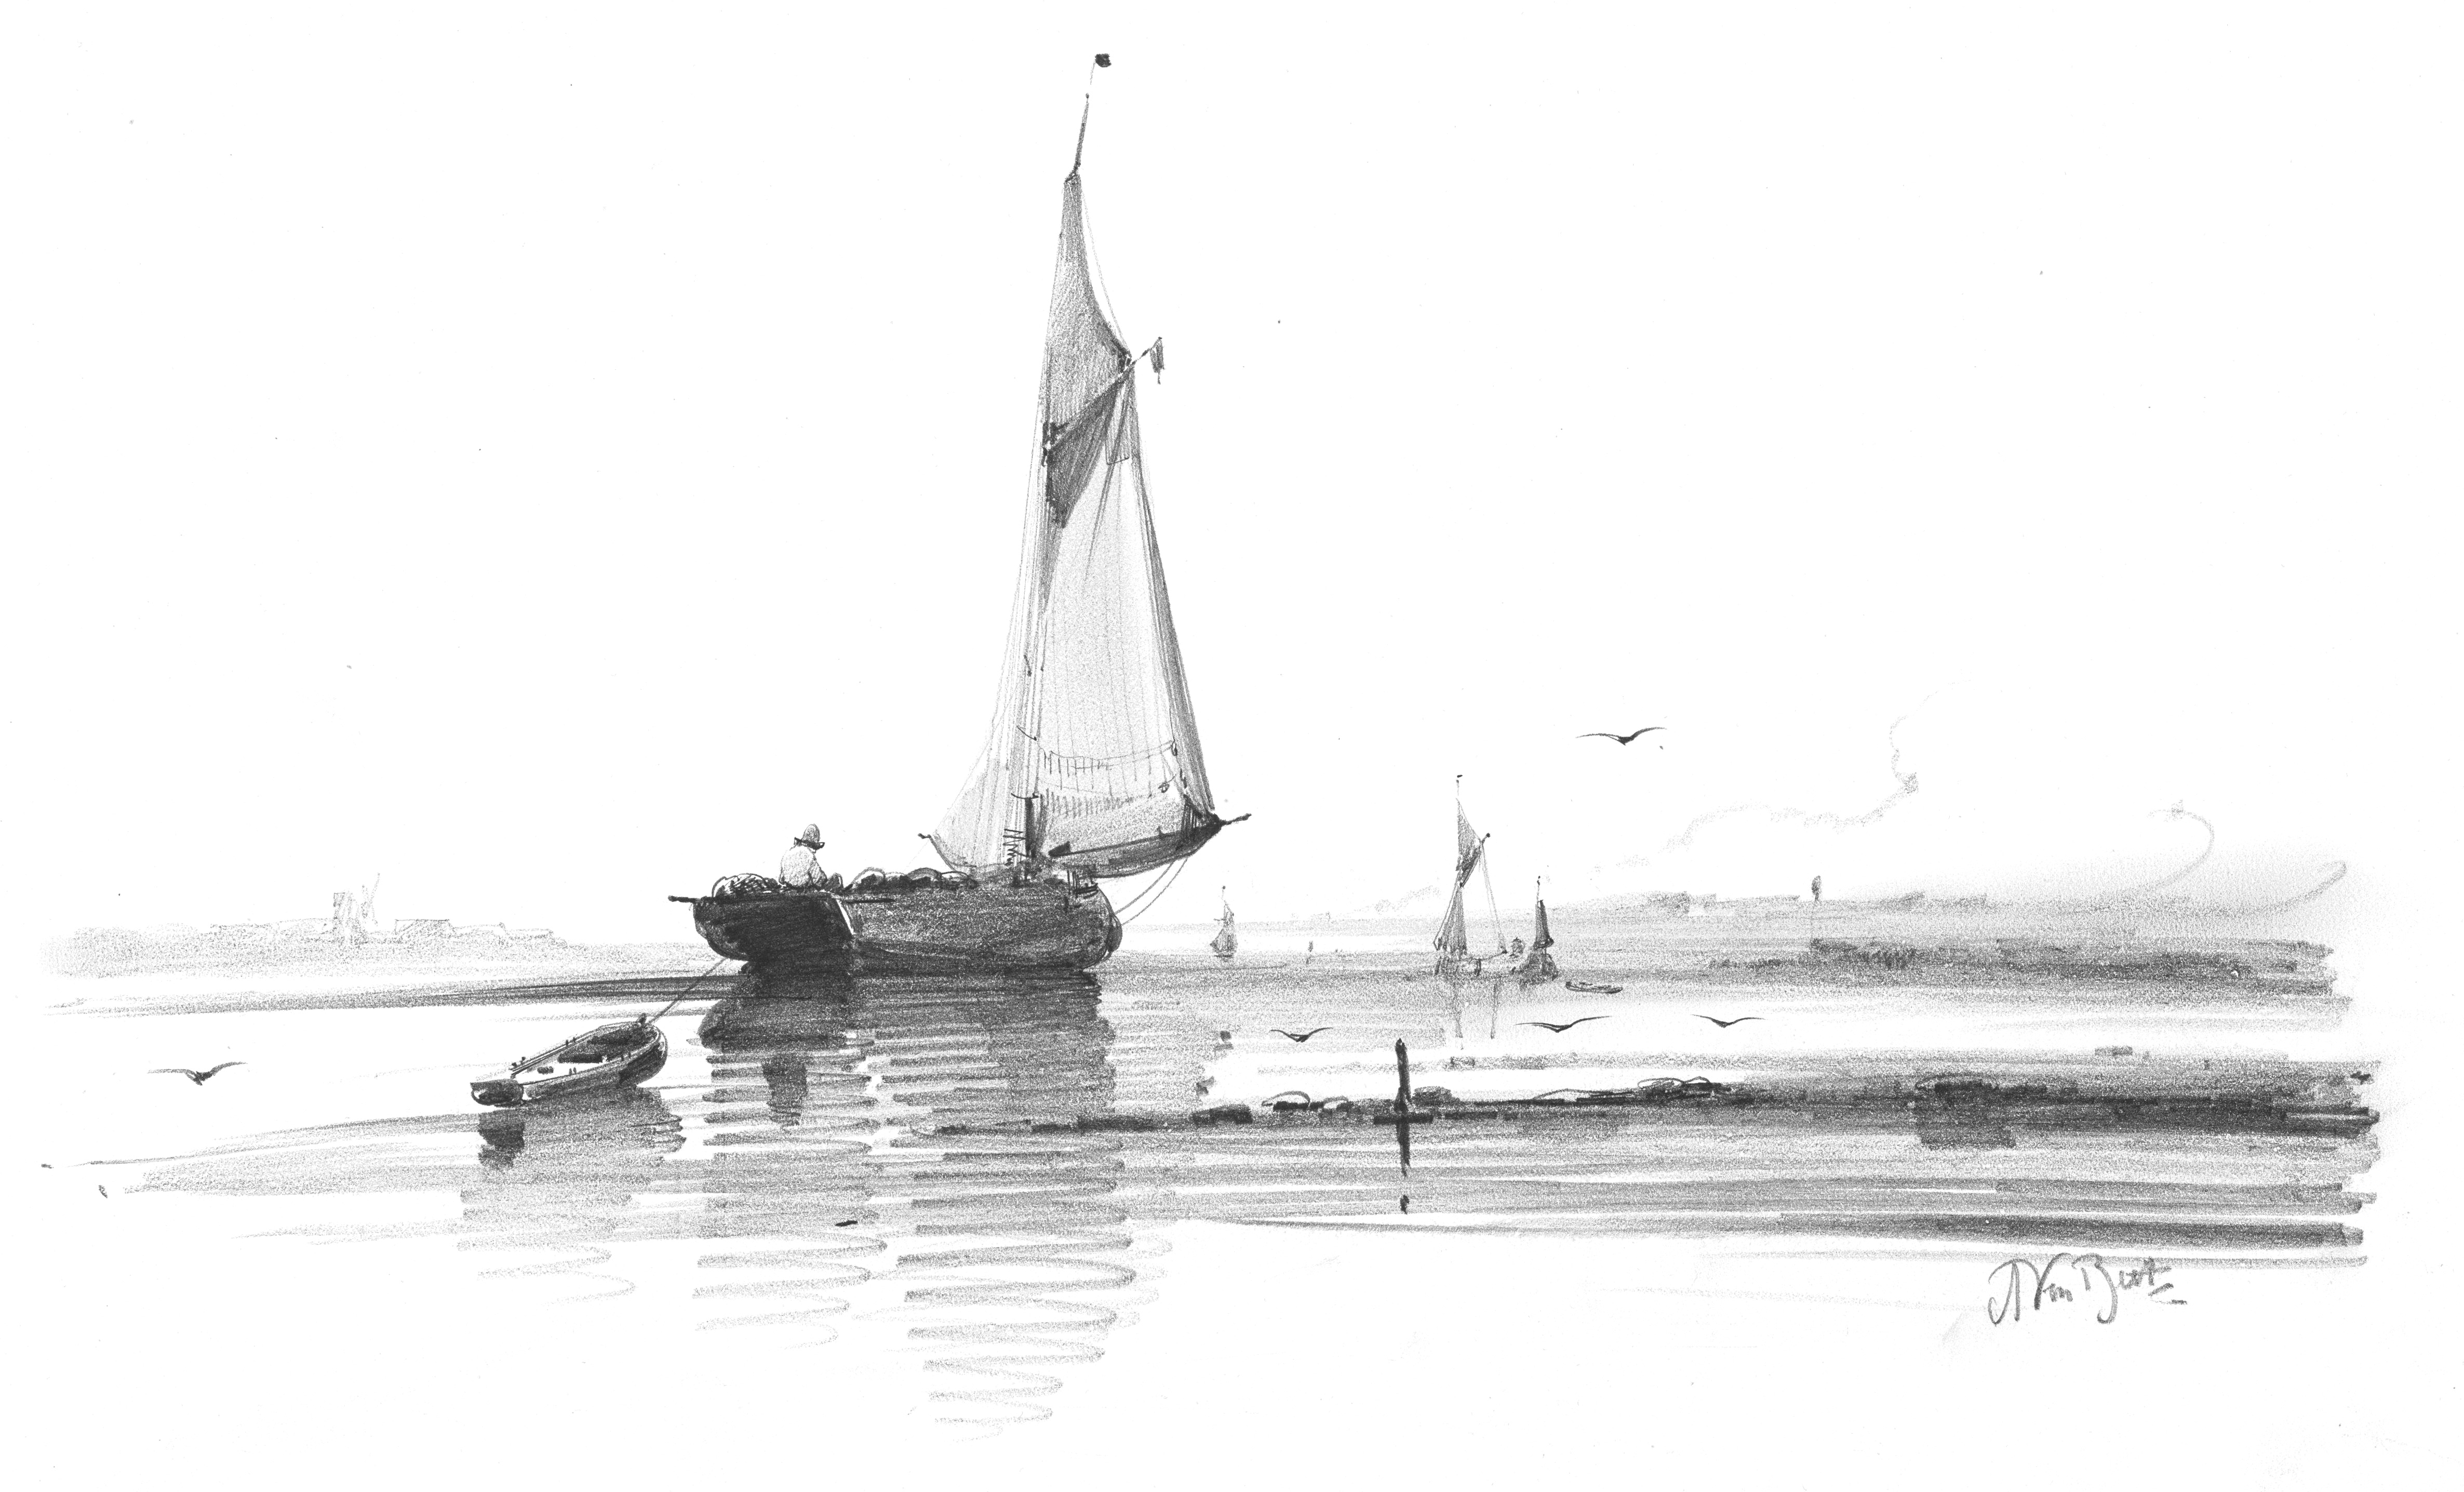
\includegraphics[width=\basicwidth]{sailboat}}
\vfill



\KOMAoptions{headings=openleft}
\chapter*{Colophon}

\centering

\vfill
\begin{minipage}{\textwidth}
\textit{Le comte de Monte-Cristo} a été publié en feuilleton dans le \textit{Journal des Débats} entre août 1844 et janvier 1846.  Comme la plupart des œuvres de Alexandre Dumas \textit{père} (1802--1870), ce fut une collaboration avec son partenaire d'écriture Auguste Maquet (1813--1888).
\end{minipage}
\vfill
gutenberg.org/ebooks/17989\\
gutenberg.org/ebooks/17990\\
gutenberg.org/ebooks/17991\\
gutenberg.org/ebooks/17992
\vfill
\divider
\vfill
\begin{minipage}{\textwidth}
Le texte est composé en <EB Garamond,> l'implémentation libre et open source par Georg Mayr-Duffner des célèbres caractères humanistes de Claude Garamond du milieu du seizième siècle. Les pages de titre sont composés en <Bolton Light,> par Paul Lloyd. Les lettrines sont composées en <Floral Capitals,> par Vladimir Nikolic. Le testament de César Spada (chapitre 18) est composé en <Essays 1743,> par John Stracke. 
\end{minipage}
\vfill
github.com/georgd/EB-Garamond\\moorstation.org/typoasis/designers/lloyd/\\www.thibault.org/fonts/essays\\
\vfill
\divider
\vfill
\begin{minipage}{\textwidth}
L'illustration des pages de titre est tiré d'un catalogue, \textit{Katalog der Ausstellung für Buchgewerbe und Photographie,} qui fut publié en 1904. Illustration de la dernière page est un dessin de Albertus van Beest (1820--1860) entitré \textit{Afgemeerde zeilboot op een kalme zee}. L'original est retenu par le Rijksmuseum d'Amsterdam.
\end{minipage}
\vfill
\divider
\vfill
\begin{minipage}{\textwidth}
Cette composition typographique est dédiée au domaine public sous une licence Creative Commons CC0 1.0 Universal: creativecommons.org/publicdomain/zero/1.0/\
\end{minipage}
\vfill
\divider
\vfill
Composé en \LaTeX{}. Dernière révision \today.
\thispagestyle{empty}

\end{document}